% *************************************
% ------- PhD Thesis Nils Eling -------
% *************************************

\documentclass[a4paper,12pt,times,numbered,print,draftclassic]{Classes/PhDThesisPSnPDF}

% *************************************
% **** Class Options 
% *************************************

% `a4paper'(The University of Cambridge PhD thesis guidelines recommends a page size a4 - default option) or `a5paper': A5 Paper size is also allowed as per the Cambridge University Engineering Deparment guidelines for PhD thesis

% `11pt' or `12pt'(default): Font Size 10pt is NOT recommended by the University guidelines

% `oneside' or `twoside'(default): Printing double side (twoside) or single side.

% `print': Use `print' for print version with appropriate margins and page layout. Leaving the options field blank will activate Online version.

% `index': For index at the end of the thesis

% `draftclassic': For draft mode without loading any images (same as draft in book)

% `draft': Special draft mode with line numbers, images, and water mark with timestamp and custom text. Position of the text can also be modified.

% `abstract': To generate only the title page and abstract page with
% dissertation title and name, to submit to the Student Registry

% `chapter`: This option enables only the specified chapter and it's references. Useful for review and corrections.

% *************************************
% **** Custom Page Margins 
% *************************************

% `custommargin`: Use `custommargin' in options to activate custom page margins, which can be defined in the preamble.tex. Custom margin will override print/online margin setup.

% *************************************
% **** Choosing the Fonts in Class Options 
% *************************************

% `times' : Times font with math support. (The Cambridge University guidelines recommend using times)

% `fourier': Utopia Font with Fourier Math font (Font has to be installed)      

% `customfont': Use `customfont' option in the document class and load the package in the preamble.tex

% default or leave empty: `Latin Modern' font will be loaded.

% *************************************
% **** Choosing the Bibliography style 
% *************************************

% `authoryear': For author-year citation eg., Krishna (2013)

% `numbered': (Default Option) For numbered and sorted citation e.g., [1,5,2]

% `custombib': Define your own bibliography style in the `preamble.tex' file. `\RequirePackage[square, sort, numbers, authoryear]{natbib}'.cThis can be also used to load biblatex instead of natbib (See Preamble)

% *************************************
% **** Choosing the Page Style 
% *************************************

% `default (leave empty)': For Page Numbers in Header (Left Even, Right Odd) and Chapter Name in Header (Right Even) and Section Name (Left Odd). Blank Footer.

% `PageStyleI': Chapter Name next & Page Number on Even Side (Left Even).  Section Name & Page Number in Header on Odd Side (Right Odd). Footer is empty.

% `PageStyleII': Chapter Name on Even Side (Left Even) in Header. Section Number and Section Name in Header on Odd Side (Right Odd). Page numbering in footer

% Uncomment to change page style
%\pagestyle{PageStyleII}

% *************************************
% **** Preamble 
% *************************************

% ******************************************************************************
% ****************************** Custom Margin *********************************

% Add `custommargin' in the document class options to use this section
% Set {innerside margin / outerside margin / topmargin / bottom margin}  and
% other page dimensions
\ifsetCustomMargin
  \RequirePackage[left=37mm,right=30mm,top=35mm,bottom=30mm]{geometry}
  \setFancyHdr % To apply fancy header after geometry package is loaded
\fi

% Add spaces between paragraphs
%\setlength{\parskip}{0.5em}
% Ragged bottom avoids extra whitespaces between paragraphs
\raggedbottom
% To remove the excess top spacing for enumeration, list and description
%\usepackage{enumitem}
%\setlist[enumerate,itemize,description]{topsep=0em}

% No indent before paragraph
\setlength\parindent{0pt}

% *****************************************************************************
% ******************* Fonts (like different typewriter fonts etc.)*************

% Add `customfont' in the document class option to use this section

\ifsetCustomFont
  % Set your custom font here and use `customfont' in options. Leave empty to
  % load computer modern font (default LaTeX font).
  %\RequirePackage{helvet}

  % For use with XeLaTeX
  %  \setmainfont[
  %    Path              = ./libertine/opentype/,
  %    Extension         = .otf,
  %    UprightFont = LinLibertine_R,
  %    BoldFont = LinLibertine_RZ, % Linux Libertine O Regular Semibold
  %    ItalicFont = LinLibertine_RI,
  %    BoldItalicFont = LinLibertine_RZI, % Linux Libertine O Regular Semibold Italic
  %  ]
  %  {libertine}
  %  % load font from system font
  %  \newfontfamily\libertinesystemfont{Linux Libertine O}
  
  % Use helvetica
  \renewcommand{\familydefault}{\sfdefault}
  \usepackage{helvet}
  \usepackage{sansmathfonts}
\fi

% *********
% ***** Custom Packages

% define header 
\usepackage{fancyhdr}
\usepackage{adjustbox}
\usepackage{etoolbox}
\renewcommand{\headrulewidth}{1pt}
\newcommand{\headrulecolor}[1]{\patchcmd{\headrule}{\hrule}{\color{#1}\hrule}{}{}}
\headrulecolor{Mahogany}
\fancyheadoffset[RE,LO]{0cm}
\fancyheadoffset[LE,RO]{1.25cm}

% For recoloring the section header
\usepackage{sectsty}
\definecolor{dark-gray}{gray}{0.30}
\sectionfont{\color{dark-gray}}
\subsectionfont{\color{dark-gray}}

% Fancier section header
\newcommand{\hsp}{\hspace{6pt}}
\usepackage[explicit]{titlesec}
\titleformat{\section}[hang]{\Large\bfseries}{\color{dark-gray}\thesection}{6pt}{\begin{tabular}[t]{@{\color{dark-gray}\vrule width 2pt}>{\hsp}l}#1\end{tabular}}
\titleformat{\subsection}[hang]{\large\bfseries}{\color{dark-gray}\thesubsection}{6pt}{\begin{tabular}[t]{@{\color{dark-gray}\vrule width 2pt}>{\hsp}l}#1\end{tabular}}



% **** Algorithms and Pseudocode 

%\usepackage{algpseudocode}


% **** Captions and Hyperreferencing / URL 

% Captions: This makes captions of figures use a boldfaced small font.
\usepackage[font=small,labelfont=bf]{caption}

%\RequirePackage[labelsep=space,tableposition=top]{caption}
\renewcommand{\figurename}{Fig.} %to support older versions of captions.sty

\usepackage{hyperref}
\hypersetup{
    colorlinks=true,
    linkcolor=black,
    filecolor=black,      
    urlcolor=Mahogany,
}


% *************************** Graphics and figures *****************************

%\usepackage{rotating}
\usepackage{wrapfig}

% Uncomment the following two lines to force Latex to place the figure.
% Use [H] when including graphics. Note 'H' instead of 'h'
%\usepackage{float}
%\restylefloat{figure}

% Subcaption package is also available in the sty folder you can use that by
% uncommenting the following line
% This is for people stuck with older versions of texlive
%\usepackage{sty/caption/subcaption}
\usepackage{subcaption}

% ********************************** Tables ************************************
\usepackage{booktabs} % For professional looking tables
\usepackage{multirow}

%\usepackage{multicol}
%\usepackage{longtable}
%\usepackage{tabularx}


% *********************************** SI Units *********************************
\usepackage{siunitx} % use this package module for SI units
\usepackage{textcomp} % for trademark


% ******************************* Line Spacing *********************************

% Choose linespacing as appropriate. Default is one-half line spacing as per the
% University guidelines

% \doublespacing
% \onehalfspacing
% \singlespacing


% ************************ Formatting / Footnote *******************************

% Don't break enumeration (etc.) across pages in an ugly manner (default 10000)
%\clubpenalty=500
%\widowpenalty=500

%\usepackage[perpage]{footmisc} %Range of footnote options

% Nicer heading
\renewcommand{\chaptername}{}
\usepackage[Lenny]{fncychap}


% *****************************************************************************
% *************************** Bibliography  and References ********************

%\usepackage{cleveref} %Referencing without need to explicitly state fig /table

% Add `custombib' in the document class option to use this section
\ifuseCustomBib
   \RequirePackage[square, sort, numbers, authoryear]{natbib} % CustomBib

% If you would like to use biblatex for your reference management, as opposed to the default `natbibpackage` pass the option `custombib` in the document class. Comment out the previous line to make sure you don't load the natbib package. Uncomment the following lines and specify the location of references.bib file

%\RequirePackage[backend=biber, style=numeric-comp, citestyle=numeric, sorting=nty, natbib=true]{biblatex}
%\addbibresource{References/references} %Location of references.bib only for biblatex, Do not omit the .bib extension from the filename.

\fi

% changes the default name `Bibliography` -> `References'
\renewcommand{\bibname}{References}


% ******************************************************************************
% ************************* User Defined Commands ******************************
% ******************************************************************************

% *********** To change the name of Table of Contents / LOF and LOT ************

%\renewcommand{\contentsname}{My Table of Contents}
%\renewcommand{\listfigurename}{My List of Figures}
%\renewcommand{\listtablename}{My List of Tables}

% Math abbreviations
\newcommand{\iid}{\stackrel{\mbox{iid}}{\sim}}
\newcommand{\ind}{\stackrel{\mbox{ind}}{\sim}}
\newcommand{\Lagr}{\mathcal{L}}
\newcommand{\plus}{\textsuperscript{+}}
\usepackage{tikz}
\def\checkmark{\tikz\fill[scale=0.4](0,.35) -- (.25,0) -- (1,.7) -- (.25,.15) -- cycle;} 



% ********************** TOC depth and numbering depth *************************

\setcounter{secnumdepth}{2}
\setcounter{tocdepth}{2}


% ******************************* Nomenclature 
%\usepackage{nomencl}
%\renewcommand{\nomname}{Symbols}
%\makenomenclature

\usepackage[acronym, nopostdot, nonumberlist, style=super]{glossaries}
%\newglossarystyle{longuc}%
%{%
%  \setglossarystyle{long}%
%  \renewcommand{\glossentry}[2]{%
%    \glsentryitem{##1}\glstarget{##1}{\glossentryname{##1}} &
%    \Glossentrydesc{##1}\glspostdescription\space ##2\tabularnewline
%  }%
%}

\setlength{\glsdescwidth}{5in}

%\newglossarystyle{clong}{%
% \renewenvironment{theglossary}%
%     {\begin{longtable}{p{.3\linewidth}p{\glsdescwidth}}}%
%     {\end{longtable}}%
%  \renewcommand*{\glossaryheader}{}%
%  \renewcommand*{\glsgroupheading}[1]{}%
%  \renewcommand*{\glossaryentryfield}[5]{%
%    \glstarget{##1}{##2} & ##3\glspostdescription\space ##5\\}%
%  \renewcommand*{\glossarysubentryfield}[6]{%
%     & \glstarget{##2}{\strut}##4\glspostdescription\space ##6\\}%
  %\renewcommand*{\glsgroupskip}{ & \\}%
%}

%\setglossarystyle{longuc}
%\setacronymstyle{long-short}

\makeglossaries
\glsdisablehyper
\renewcommand{\glsnamefont}[1]{\textbf{#1}}

% ********************************* Appendix 

% The default value of both \appendixtocname and \appendixpagename is `Appendices'. These names can all be changed via:

%\renewcommand{\appendixtocname}{List of appendices}
%\renewcommand{\appendixname}{Appndx}

% *********************** Configure Draft Mode **********************************

% Uncomment to disable figures in `draft'
%\setkeys{Gin}{draft=true}  % set draft to false to enable figures in `draft'

% These options are active only during the draft mode
% Default text is "Draft"
%\SetDraftText{DRAFT}

% Default Watermark location is top. Location (top/bottom)
%\SetDraftWMPosition{bottom}

% Draft Version - default is v1.0
%\SetDraftVersion{v1.1}

% Draft Text grayscale value (should be between 0-black and 1-white)
% Default value is 0.75
%\SetDraftGrayScale{0.8}


% ******************************** Todo Notes **********************************

% Define colour for todo notes
\newcommand{\todo}[1]{{\color{red}{#1}}}

% *****************************************************************************
% ******************* Better enumeration my MB*************
\usepackage{enumitem}

% **********************************
% Additional packages
\usepackage{xcolor}
\definecolor{green}{RGB}{32,157,148}
\usepackage{amsmath,amsfonts,amssymb,amsthm,nccmath} % For math equations, theorems, symbols, etc
\usepackage{bm} % bold math 
\usepackage{textgreek} % greek letters in text

%----------------------------------------------------------------------------------------
%	THEOREM STYLES
%----------------------------------------------------------------------------------------

%%%%%%%%%%%%%%%%%%%%%%%%%%%%%%%%%%%%%%%%%%%%%%%%%%%%%%%%%
%%% dedicated to boxed/framed environements %%%%%%%%%%%%%
%%%%%%%%%%%%%%%%%%%%%%%%%%%%%%%%%%%%%%%%%%%%%%%%%%%%%%%%%

\newtheoremstyle{greennumbox}% % Theorem style name
{0pt}% Space above
{0pt}% Space below
{\small}% % Body font
{}% Indent amount
{\small\bf\sffamily\color{green}}% % Theorem head font
{\;}% Punctuation after theorem head
{0.25em}% Space after theorem head
{\small\sffamily\color{green}\thmname{}\nobreakspace} 
\renewcommand{\qedsymbol}{$\blacksquare$}% Optional qed square

\newtheoremstyle{blacknumbox} % Theorem style name
{0pt}% Space above
{0pt}% Space below
{\normalfont}% Body font
{}% Indent amount
{\small\bf\sffamily}% Theorem head font
{}% Punctuation after theorem head
{0.25em}% Space after theorem head
{\small\sffamily\thmname{}\nobreakspace}

% Defines the theorem text style for each type of theorem to one of the three styles above
\theoremstyle{greennumbox}
\newtheorem{abstractT}{}
\theoremstyle{blacknumbox}
\newtheorem{commentT}{}


% Package to create coloured boxes
\RequirePackage[framemethod=default]{mdframed}

% Exercise box	  
\newmdenv[skipabove=7pt,
skipbelow=7pt,
rightline=false,
leftline=true,
topline=false,
bottomline=false,
backgroundcolor=green!10,
linecolor=green,
innerleftmargin=5pt,
innerrightmargin=5pt,
innertopmargin=5pt,
innerbottommargin=5pt,
leftmargin=0cm,
rightmargin=0cm,
linewidth=4pt]{eBox}	

\newmdenv[skipabove=7pt,
skipbelow=7pt,
rightline=false,
leftline=true,
topline=false,
bottomline=false,
linecolor=gray,
backgroundcolor=black!5,
innerleftmargin=5pt,
innerrightmargin=5pt,
innertopmargin=5pt,
leftmargin=0cm,
rightmargin=0cm,
linewidth=4pt,
innerbottommargin=5pt]{cBox}

% Creates an environment for each type of theorem and assigns it a theorem text style from the "Theorem Styles" section above and a colored box from above
\newenvironment{Abstract}{\begin{eBox}\begin{abstractT}}{\hfill{\color{green}\tiny\ensuremath{\blacksquare}}\end{abstractT}\end{eBox}}				  		
\newenvironment{Comment}{\begin{cBox}\begin{commentT}}{\end{commentT}\end{cBox}}	


%!TEX root = ../main.tex
%******************************
%	 Acronym 
%*****************************

\newacronym{Th}{Th}{T-helper} 
\newacronym{scRNA-Seq}{scRNA-Seq}{Single-cell RNA Sequencing} 
\newacronym{mRNA}{mRNA}{messenger RNA} 
\newacronym{HIV}{HIV}{Human Immunodeficiency Virus} 
\newacronym{lambdaPhage}{$\lambda$-phage}{Lambda phage} 
\newacronym{Bsubtilis}{\emph{B.~subtilis}}{\textit{Bacillus subtilis}}
\newacronym{Ecoli}{\emph{E.~coli}}{\textit{Escherichia coli}}
\newacronym{Oct4}{Oct4}{Octamer-binding transcription factor 4}
\newacronym{Sox2}{Sox2}{Sex determining region Y-box 2}
\newacronym{H3R26}{H3R26}{Histone H3 arginine-26}
\newacronym{Carm1}{Carm1}{Coactivator associated arginine methyltransferase 1 }
\newacronym{E}{E}{Embryonic day}
\newacronym{ICM}{ICM}{Inner Cell Mass}
\newacronym{mESC}{mESC}{mouse Embryonic Stem Cells}
\newacronym{iPSC}{iPSC}{induced Pluripotent Stem Cell}
\newacronym{Ifn}{Ifn}{Interferone}
\newacronym{Il}{Il}{Interleukine}
\newacronym{Tbx21}{Tbx21}{T-Box 21}
\newacronym{Gata}{Gata}{GATA binding protein}
\newacronym{LPS}{LPS}{Lipopolysaccharide}
\newacronym{NFkB}{NF-$\kappa$B}{Nuclear Factor kappa-light-chain-enhancer of activated B cells}
\newacronym{LIF}{LIF}{Leukemia Inhibitory Factor}
\newacronym{Celegans}{\textit{C. elegans}}{\textit{Caenorhabditis elegans}}
\newacronym{TRAIL}{TRAIL}{TNF-related apoptosis-inducing ligand}
%\newacronym{}{}{}


% *************************************
% **** Thesis Information & Meta-data 
% *************************************

% *************************************
% **** Thesis Information & Meta-data 
% *************************************

%% The title of the thesis
\title{Quantifying expression variability
 in\\ single-cell RNA sequencing data}

%% The full name of the author
\author{Nils Eling}

%% Department (eg. Department of Engineering, Maths, Physics)
\dept{European Molecular Biology Laboratory, \\ European Bioinformatics Institute}

%% University and Crest
\university{University of Cambridge}
% Crest minimum should be 30mm.
\crest{\includegraphics[width=0.2\textwidth]{University_Crest}}

%% Full title of the Degree
\degreetitle{Doctor of Philosophy}

%% College affiliation (optional)
\college{Pembroke College}

%% Submission date
% Default is set as {\monthname[\the\month]\space\the\year}
\degreedate{February 2019} 

% *************************************
% ***** Abstract 
% *************************************

\ifdefineAbstract
 \pagestyle{empty}
 \includeonly{Declaration/declaration, Abstract/abstract}
\fi

% *************************************
% **** Chapter Mode 
% *************************************
% The chapter mode allows user to only print particular chapters with references. Title, Contents, Frontmatter are disabled by default. Useful option to review a particular chapter or to send it to supervisior. To use choose `chapter' option in the document class

\ifdefineChapter
 \includeonly{Introduction/intro}
\fi

% *************************************
% **** Front Matter 
% *************************************

\begin{document}

\frontmatter

\maketitle

%% ***** Thesis Dedidcation 

\begin{dedication} 

\textit{Ich widme diese Arbeit meiner Familie - Hildegard, J\"org und Laura - und bedanke mich f\"ur eure Unterst\"utzung und Geduld w\"ahrend meiner Promotion.}

\end{dedication}


%% ******************************* Thesis Declaration ***************************

\begin{declaration}

This dissertation is my own work and contains nothing which is the outcome of work done in collaboration with others, except as specified in the individual declarations at the beginning of each chapter and the outline. It is not substantially the same as any that I have submitted, or, is being concurrently submitted for a degree or diploma or other qualification at the University of Cambridge or any other University or similar institution. I further state that no substantial part of my dissertation has already been submitted, or, is being concurrently submitted for any such degree, diploma or other qualification at the University of Cambridge or any other University or similar institution. This dissertation contains fewer than 60,000 words exclusive of tables, footnotes, bibliography, and appendices and has fewer than 150 figures.
\end{declaration}


%% **** Thesis Acknowledgements

\begin{acknowledgements}      


First and foremost, I want to thank my supervisor John Marioni for offering me to work in his research group. John took the risk in supervising me as a PhD student from a wet-lab background and introduced me to statistical analyses. I'm thankful for all his enthusiasm and support which guided me to successfully finishing my PhD. I also want to thank Catalina Vallejos for supervising me and turning me into a "Bayesian statistician". Not only did she support my work but also as a good friend. \\

This whole work builds on excellent collaborations. I want to thank Duncan Odom not only for allowing me to work with his lab but also for guiding me through important career-related processes (e.g.~paper writing). Christina Ernst supported large parts of this work with experiments, data interpretation and late nights of paper writing. I also want to thank Celia Martinez-Jimenez for large-scale experimental support. Furthermore, I thank Detlev Arendt and Kaia Achim for collaborating on an early project during my PhD. Maike de la Roche and Hung-Chang Chen played a crucial role for publishing the final version of the immune ageing project. My thesis advisory committee members, Sarah Teichmann, Wolfgang Huber and Duncan Odom provided fruitful discussions that advanced my research during over the last four years. \\

All current and former lab members of the Marioni lab deserve a huge thanks for providing such a pleasant and stimulating work environment. I specifically thank: Aaron Lun for his statistical support, entertainment and being a BK lunch companion; Michael Morgan for discussing what "noise" really means; Arianne Richard for biological insights into the confusing world of T cells. I also thank Anna, Chris, Luis, Antonio, Konrad, Catalina, Liora, Jonny, Tom, Ximena, Christina, and Rebecca for all the fun times during the last four years. \\

A special thanks also goes to people who read and commented on this thesis: Christina Ernst, Jack Monahan, Hannah Meyer, Michael Morgan, Catalina Vallejos, and John Marioni. 

\newpage
\thispagestyle{empty}
 

Importantly, I want to thank my friends from Cambridge, Heidelberg and Essen for their moral support, keeping me sane during stressful times and . Hannah, Omar, Catalina, Jack, Christina, Dani, Julia

Friends: Christina, Hannah, Jack, Dani, Lara, Omar, Julia, Ruben,  Sebastian, Felix, Fabian, Jonathan, Georg. The guys from Essen

Pembroke rowing

climbing

Bodi

\end{acknowledgements}

%% ***********************************
% **** Thesis Abstract 
% ***********************************

\begin{abstract}
Transcriptional noise is an intrinsic feature of cell populations and plays a driving role in mammalian development, tissue homoeostasis and immune function. While expression heterogeneity, a phenotypic readout of transcriptional noise, has been broadly studied in prokaryotic model systems or by profiling individual genes, few whole-transcriptome studies in mammalian systems have been reported. The development of single-cell RNA sequencing technologies introduced powerful tools to investigated transcriptional differences between individual cells, therefore allowing the in-depth characterization of expression variability. In this thesis, I computationally analysed single-cell RNA sequencing data to understand transcriptional variability  and expanded a statistical model to avoid confounding effects when quantifying such variability. First, I profiled individual transcriptomes  of CD4\plus{} T cells to identify a global decrease in transcriptional variability upon immune activation. By extending this analysis across two sub-species of mice, I identified an evolutionarily conserved set of immune response genes for which transcriptional variability increases during ageing. I used a Bayesian modelling framework to quantify mean expression and transcriptional variability but due to a strong confounding effect between these two parameters, variability analysis was restricted to genes that are similarly expressed across the tested conditions. To address this problem, I extended the existing BASiCS framework allowing the parallel assessment of changes in mean expression and variability. Within this Bayesian framework, I introduced a joint prior specification effecting mean expression and variability parameters to calculate a residual over-dispersion measure for each gene. This measure allows me to statistically assess changes in variability even for genes with differences in mean expression between conditions. Finally, I applied this model to identify temporal changes in variability over the time-course of spermatogenesis. This unidirectional differentiation process involves several complex steps to form mature sperm from spermatogonial stem cells. When profiling changes in variability across this developmental time-course, peaks in variability are caused by rapid changes in gene expression along the differentiation trajectory. This thesis provides a deeper understanding of technical and biological factors that drive transcriptional variability and offers a basis for future research to characterize its role in health and disease.
\end{abstract}


% *************************************
% **** Adding TOC and List of Figures 
% *************************************

\cleardoublepage

\tableofcontents

\cleardoublepage

\listoffigures

\cleardoublepage

\listoftables

\renewcommand{\glossarypreamble}{\vspace{-2cm}}
\printglossary[type=\acronymtype, toctitle=Acronyms, title=\textcolor{Mahogany}{\LARGE{\textbf{\textsc{Acronyms}}}}]
\addcontentsline{toc}{chapter}{Acronyms}

% *************************************
% **** Main Matter
% ************************************* 

\mainmatter


%!TEX root = ../main.tex
%******************************
%	 Introduction 
%*****************************

\chapter{Introduction}  

\graphicspath{Figures/}

\begin{Abstract}
The intrinsic stochasticity of biochemical reactions introduces phenotypic heterogeneity in seemingly homogeneous populations of cells. This phenomenon has been widely studied in prokaryotic and eukaryotic systems and the functional role of phenotypic variation in development, health and disease is the subject of ongoing research. Biological noise, a term to describe variability between individual cells, arises from different sources in homogeneous cell populations. Intrinsic noise summarizes stochastic differences in transcription and translation between individual genes \citep{Elowitz2002, Raser2004, Sanchez2013}. Extrinsic noise arises when cells are in different cellular states (e.g. cell cycle, cell-to-cell signalling and metabolism) within a homogeneous population \citep{Zopf2013, Iwamoto2016, Kiviet2014}.  \\
Recent technological advances allow the in depth analysis of biological noise in cell populations. Imaging methodologies \citep{Moffitt2016a} and single-cell “omics” techniques \citep{Bock2016} permit the quantification of thousands of mRNA species, the genomic sequence, its epigenetic modification, and selected sets of proteins per cell. Moreover, the development of multi-omics technologies opens the possibility to link cell-to-cell variation between multiple regulatory layers across individual cells \citep{Macaulay2017}. With the emergence of scRNAseq technologies, new computational strategies to quantify noise were introduced \cite{Brennecke2013, Vallejos2015, Kolodziejczyk2015cell, Buettner2015, Fan2015, Richard2016}. \\
Applying high-throughput scRNAseq to mammalian systems characterised the functional role of biological noise in healthy as well as diseased contexts. Studies of recent years described changes in noise levels at different stages during embryonic development which hints at stochastic contributions to early cell fate decisions \citep{Goolam2016, Mohammed2017, Ohnishi2014}. Phenotypic variation in immune cells, possibly derived by transcriptional noise, increases cellular plasticity and facilitates the population response to pathogens \citep{Shalek2014, Kellogg2015a}. Conversely, genetic and non-genetic heterogeneity within cell populations was described as driver for cancer development \citep{Marusyk2012} and noise increases with age \citep{Martinez-jimenez2017, Enge2017}.\\
In the introduction, I introduce noise as an inherent feature of biological system and discuss positive and negative consequences of noise in cell populations. Furthermore, I outline recent developments of single-cell sequencing and imaging technologies and comment on robust ways of quantifying biological noise. 
\end{Abstract}

\nomenclature[z-cif]{$CIF$}{Cauchy's Integral Formula}                                % first letter Z is for Acronyms 
% first letter A is for Roman symbols
% first letter G is for Greek Symbols
% first letter G is for Greek Symbols
% first letter G is for Greek Symbols
% first letter X is for Other Symbols
% first letter R is for superscripts
% first letter S is for subscripts

\newpage

% Include different main sections of the introduction
Kello%!TEX root = ../intro.tex
%******************************
%	 Biological noise 
%*****************************

\section{Biology of expression noise} 

\cor{The intrinsic stochasticity of biochemical reactions contributes to a wide distribution of \glspl{mRNA} and proteins across a seemingly homogeneous populations of cells\citep{Elowitz2002}. 
In the scientific litearature, this phenomenon is referred to as “biological noise” (see \textbf{Box 1})}
All cellular systems are exposed to varying levels of noise and employ strategies to make use of or cope with this source of variation. 
The sources and consequences of biological noise have been studied in an array of viral, prokaryotic and eukaryotic systems \citep{Raj2010, Balazsi2011, Eldar2010}. 
Across these systems the extent of its function remains unclear. 

\begin{Comment}
\hspace{-2.5mm}\textbf{Box 1: Defining biological noise}\label{box1}\\
\small
Biological noise in cell populations \cor{is defined as} stochastic effects on transcription and translation that propagates to form cell-to-cell phenotypic differences. 
To \cor{understand} noise, one needs to distinguish between different sources of cell-to-cell variability in multiple measurable factors. 
On the broadest level, differences between single cells in a population can arise from structured and unstructured sources. 
When capturing cell populations that contain discrete cell states and/or cell types \citep{Paul2015, Ibarra-Soria2018, Rosenberg2018}, measuring cell-specific features results in the detection of non-stochastic but rather correlated (structured) differences between individual cells. 
When the cell population structure is not driven by correlated features (unstructured variation), continuous processes (e.g.~differentiation) can be the dominating source of cell-to-cell phenotypic variability \citep{Dahlin2018}. 
Computational approaches allow the detection of these trajectories (e.g.~via \gls{PCA} or pseudotime inference \citep{Trapnell2014, Angerer2015}). 
Therefore, \cor{my work and work of others \citep{Faure2017, Morgan2018} focus on studying "molecular phenotypic variability", independent of measurement errors, in homogeneous cell populations as proxy for biological noise}. \\

\cor{Classically and specifically in populations of bacteria} \citep{Elowitz2002}, biological noise has broadly been classified into intrinsic and extrinsic noise. 
Intrinsic noise originates from stochastic biochemical effects that directly influence mRNA and protein expression gene-specifically (e.g.~\gls{TF} binding dynamics, see \citep{Swain2002}). 
Extrinsic noise on the other hand introduces co-variation across multiple genes (also in a pathway specific manner \citep{Raser2005}) due to \cor{variations} in cell-specific factors such as stress response, mitochondrial maintenance, amino-acid synthesis \citep{Stewart-Ornstein2012} or cell cycle \citep{Zopf2013}. 
\cor{Within a population of bacteria,} intrinsic noise can therefore be measured as expression differences between co-regulated genes in one cell, while extrinsic noise is measured as co-regulated variance in gene sets across all cells.
\cor{In multicellular systems however, the observed molecular phenotypic variability is a combination of stochastic (noise) and deterministic effects, which are difficult to delineate.}
\end{Comment}

\newpage

It is crucial to differentiate between unicellular systems (prokaryotes, viruses, and yeast) in which biological noise supports responses to environmental changes and higher, multicellular eukaryotic systems where biological noise either benefits or obstructs cellular function depending on the tissue type and health state. 
\cor{Furthermore, measuring the stochastic component of biological noise is difficult and requires time-resolved reporter gene read-outs in truly homogeneous cell populations\citep{Elowitz2002}. 
Due to this, the majority of studies presented in this chapter use the observable molecular phenotypic variation in form of single-cell transcriptomic or proteomic read-outs as proxy for biological noise (see \textbf{Box 1}). 
This variation is confounded by unobserved deterministic processes (e.g subtle cell cycle variation) and delineating the stochastic and deterministic component is challenging.}

\subsection{Bet-hedging in unicellular systems}

Biological noise has been \cor{proposed} to trigger the differential decision between latency and replication in viruses such as \gls{HIV} and the $\lambda$-phage. 
In the case of the $\lambda$-phage, infected cells either reside in a lysogenic state where the genetic material of the virus is transmitted to daughter cells without inducing cell death, or a lytic state where the virus destroys the host cell \textbf{(Fig.~\ref{fig0:bedhedging})} \citep{Lieb1953}. 
Previous studies have shown that the lysis-lysogeny switch in $\lambda$-phage is driven by intrinsic and extrinsic noise \citep{Arkin1998, St-Pierre2008}. 
This idea has been extended by Zeng \textit{el al.}, 2010 where the lysis-lysogeny switch does not depend on a single noise-driven decision but on the sum of all individual phages per cell \citep{Zeng2010}. 
\cor{This results contradicts the earlier studies, which either modelled the decision event on the level of each phage or connected the decision event with cellular volume. 
In general, by summing across stochastic events or if one is able to predict the lysis-lysogeny decision based on cellular volume, the switch does not occur as stochastically as initially anticipated.}
In the case of \Gls{HIV}, the virus either rapidly replicates or resides in a long-lived latent state from which the virus can switch to replication \citep{Weinberger2015}. 
It has been shown that combining noise-enhancing and activating drugs shifts latent viruses into the active-replication state that can be targeted by anti-retroviral therapeutics \citep{Dar2014}. 
\cor{Independent of the stochastic contribution to the latency-replication switch, this study present one of the first approaches to modulate phenotypic variability of a biological system to enhance therapeutic efficiency.}

\begin{figure}[!h]
\centering
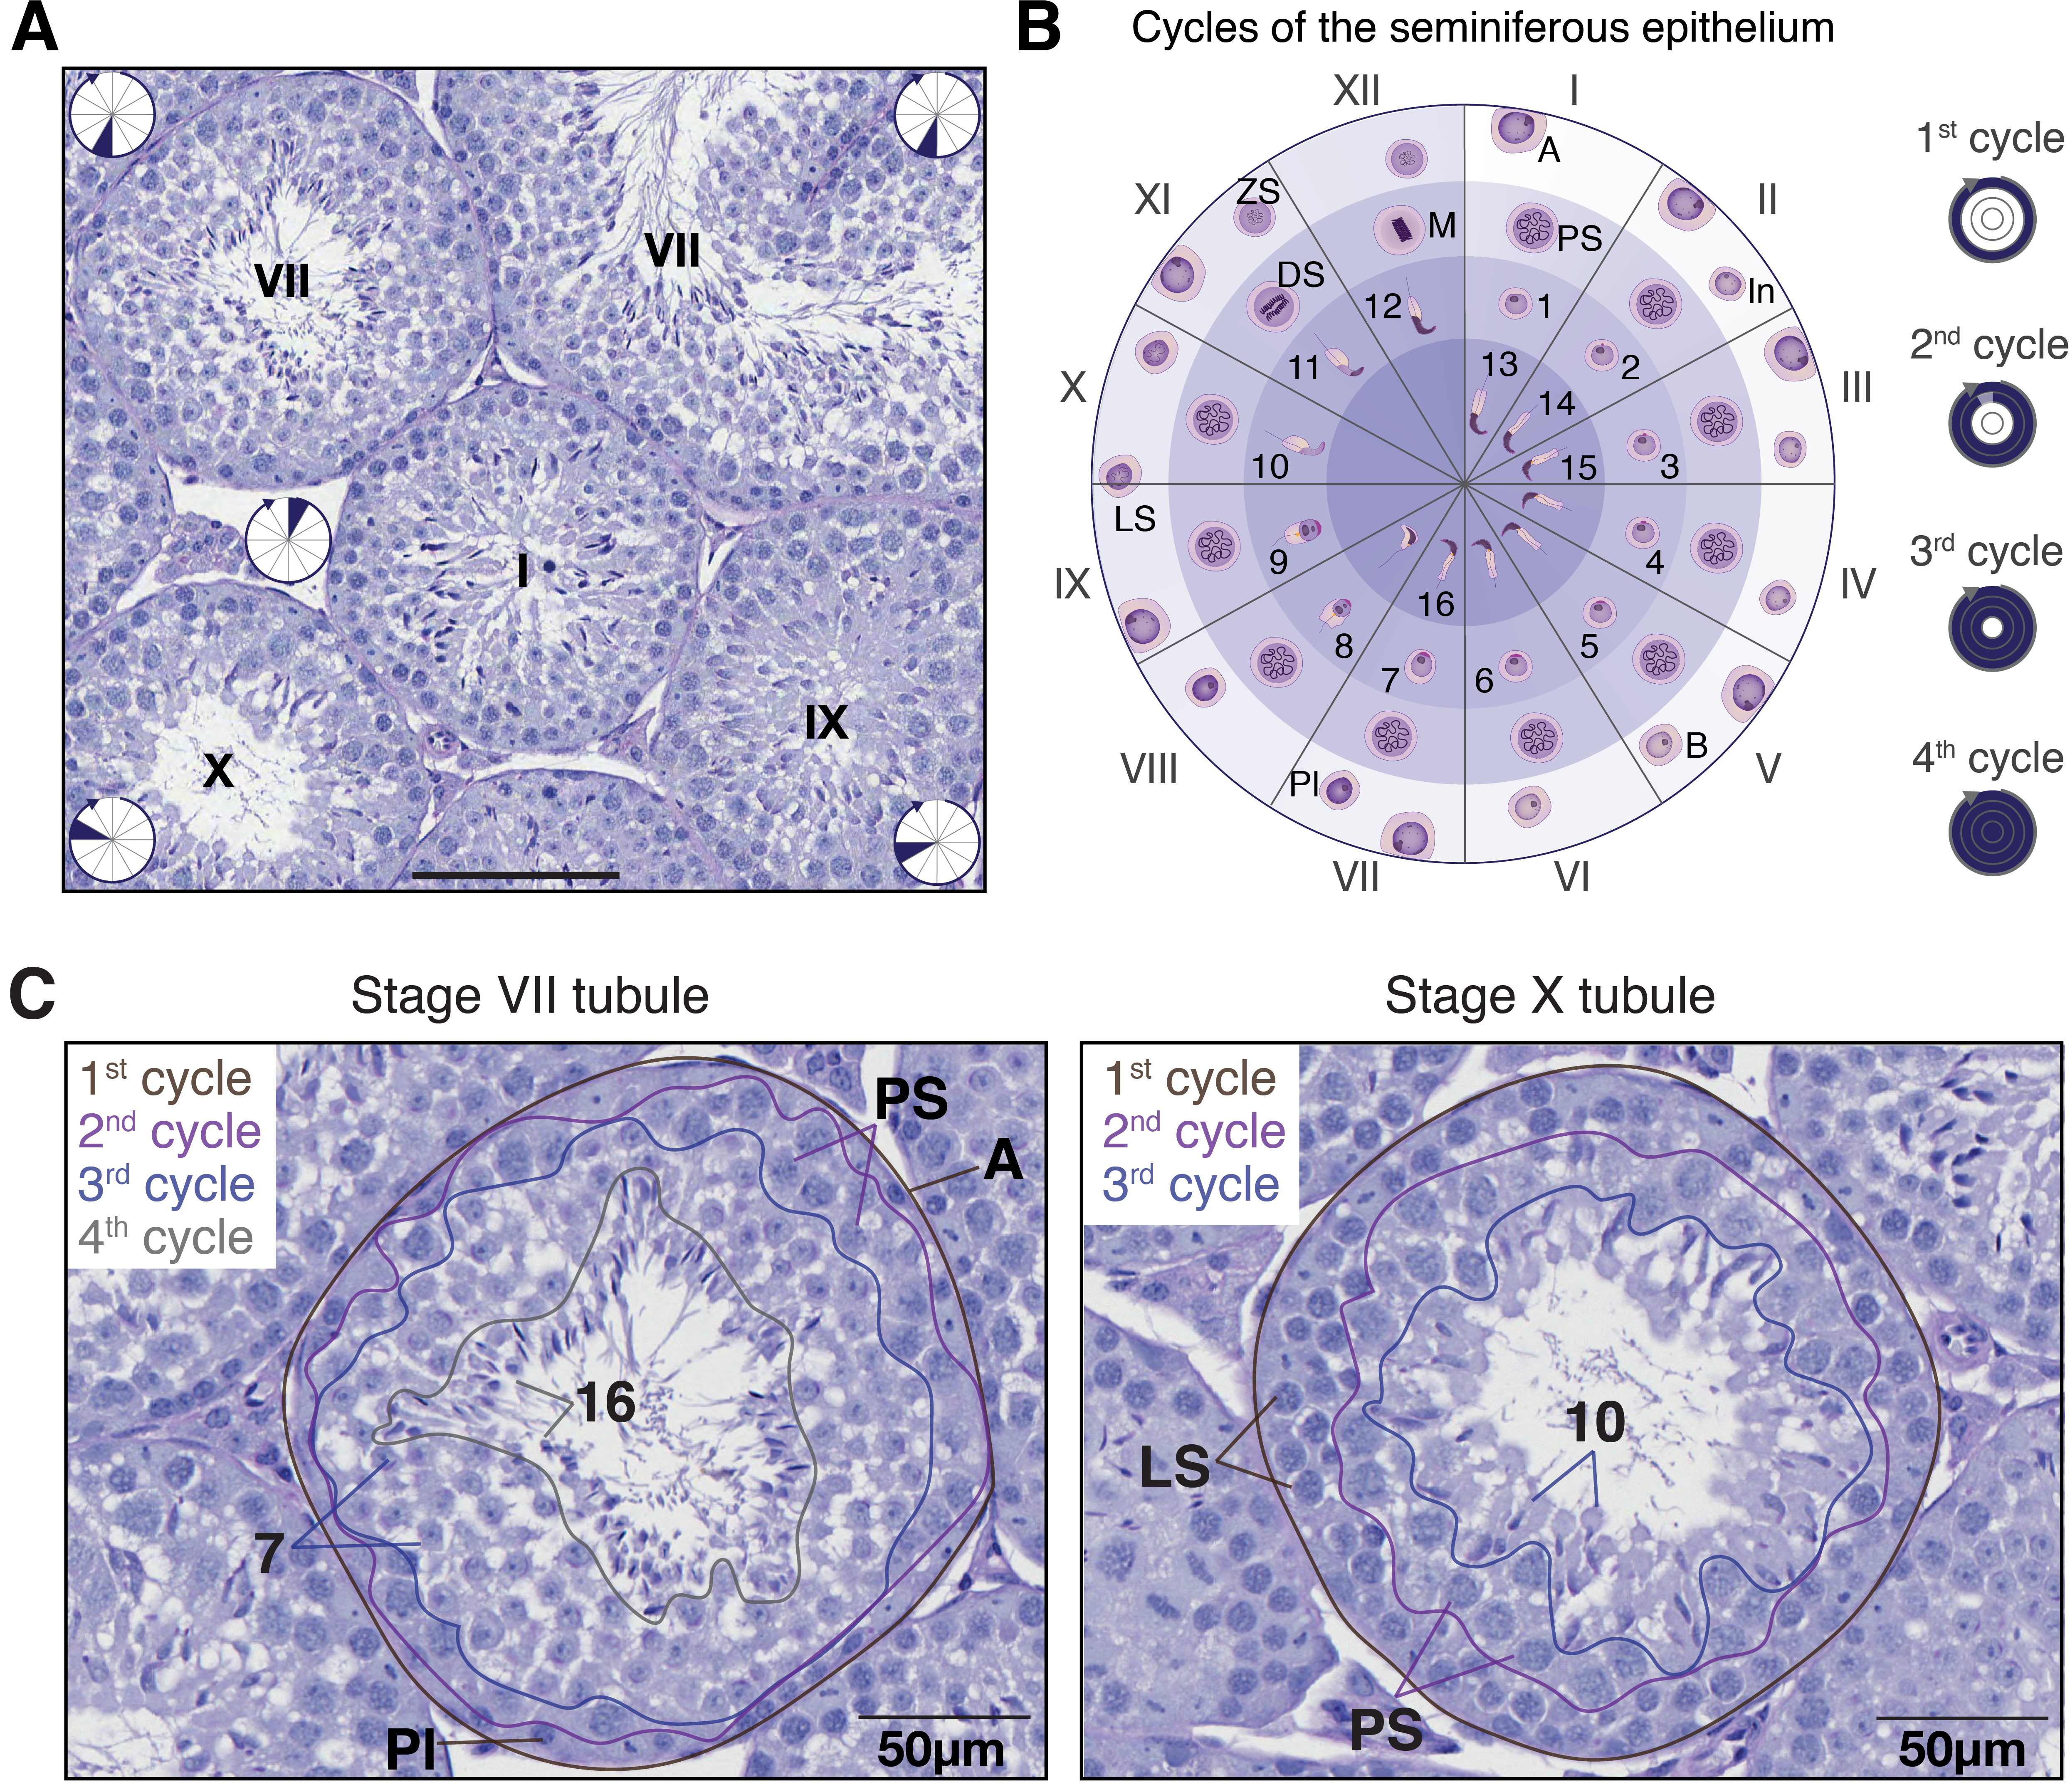
\includegraphics[width=\textwidth]{Fig_1.png}
\caption[Bet-hedging strategy of the $\lambda$-phage]{\textbf{Bet-hedging strategy of the $\lambda$-phage.}\\
The linear genome of the $\lambda$-phage enters the \Gls{Ecoli} host cell and circularises. 
A stochastic decision is made to enter the (i) lytic or (ii) lysogenic cycle where (i) the $\lambda$-phage genome replicates, the $\lambda$-phage particles assemble in the host cell and the cell is destroyed releasing the virions or (ii) the $\lambda$-phage is integrated into the host genome (prophage) and transferred to daughter cells during cell divisions. 
Under stress conditions, the $\lambda$-phage genome is excised from the host genome and enters the lytic cycle.}
\label{fig0:bedhedging}
\end{figure}

In unicellular organisms, \cor{biological noise has been linked to ‘bet-hedging’ strategies, where a sub-optimal fitness landscape is tolerated across a population of cells in order to facilitate an effective response to environmental changes.}. Here, phenotypic heterogeneity facilitates the commitment to alternative cell states in cases of stress (e.g.~nutrient deprivation, temperature fluctuations). 
For example, \Gls{Bsubtilis} either commits to sporulation or competence upon starvation or DNA damage. 
Sporulation describes an irreversible process during which vegetative growth ends and the cell forms endospores that survive the altered environment. 
Competent bacteria on the other hand take up DNA from endospores to repair DNA damage \citep{Schultz2009}. 
The probabilistic and transient activation of competence in a sub-population of \Gls{Bsubtilis} cells is modulated by fluctuations in the competence regulators ComK and ComS. 
An excitable system of negative and positive feedback loops controls the number of cells that reversibly commit to competence while other cells irreversibly execute sporulation \citep{Suel2006}. 
\cor{Variations} in the process of transferring phoshporyl groups across a cascade of regulators maintains a constant probability for cells committing to sporulation under nutrient deprived conditions \citep{Russell2017}. 
A similar phenomenon is observed in \Gls{Ecoli} populations exposed to antibiotics where pre-existing phenotypic heterogeneity allows some cells to resist antibiotic treatment. 
Once regrown, these cells remain sensitive to the antibiotic \citep{Balaban2004}. \\

Similar to phenotypic heterogeneity in unicellular prokaryotes, transcriptional noise facilitates the switching between mating phenotypes in yeast upon exposure to pheromones \citep{Paliwal2007}. 
Comparably, commitment to utilising galactose as a nutrient source is a cell fate transition, which is facilitated by stochastic gene expression \cite{Acar2008}. \\

\cor{In these systems, biological noise introduces variation in mRNA and proteins that increase plasticity for cells to adapt to changeing environments.
However, to control and balance the number of cells that commit to a specific fate, noise needs to be buffered as observed in the regulatory network of feedback loops controlling sporulation and competence.}

\subsection{Development and differentiation}

Similar to bet-hedging strategies in unicellular organisms, noise can facilitate the switch between cell states and the probabilistic induction of differentiation processes \citep{Eldar2010, Chang2008}.
\cor{However, as mentioned above, measuring biological noise in differentiating multi-cellular organisms is challenging and the observed molecular phenotypic variability is a combination of stochastic and deterministic components.} 
It has been shown that transcriptional \cor{variability} increases throughout differentiation \citep{Stumpf2017} and development \citep{Antolovic2017}. 
Dissecting differentiation processes of haematopoietic progenitor cells revealed an increase in transcriptional \cor{variability} directly before cell fate decisions are made \citep{Mojtahedi2016, Richard2016}. 
Once committed, differentiating cell populations collapse in variability and move towards a new attractor state. 
\cor{These studies highlight a possible contribution of molecular variability to cell fate decision event.
However, the observed change in variability within differentiating cell populations is purely correlative and it is not possible, with these experiments, to differentiate between variability causing differentiation or differentiation causing variability.}\\

Studies of recent years proposed that stochasticity in expression \cor{contributes to} early (pre-implantation) embryonic development, and to gastrulation \citep{Dietrich2007}. 
As early as the 4-cell stage embryo, targets of master pluripotency factors Oct4 and Sox2 are heterogeneously expressed \textbf{(Fig.~\ref{fig0:noise_development}, left panel)}. 
This is caused by heterogeneous methylation patterns of \gls{H3R26} induced by \gls{Carm1}, which in turn facilitates the binding of Oct4 and Sox2 to induce pluripotency. 
Cells with unmethylated H3R26 differentiate towards the extra-embryonic trophoectoderm while pluripotent cells form the inner cell mass \citep{Goolam2016}. 
Once the cells compact at \gls{E} 3.5, cells of the \gls{ICM} stochastically express genes to initiate heterogeneity within the cell population \textbf{(Fig.~\ref{fig0:noise_development}, 2\textsuperscript{nd} panel)}. 
Fgf4 driven signal reinforcement controls this heterogeneity to form a salt-and-pepper like cell state pattern at E3.5. 
Positional information and the establishment of gene regulatory networks facilitate the segregation of the epiblast and primitive endoderm lineage at E4.5 \textbf{(Fig.~\ref{fig0:noise_development}, 3\textsuperscript{rd} panel)} \citep{Ohnishi2014}. 
In line with this, scRNA-Seq revealed high levels of \cor{transcriptional variability} in the uncommitted inner cell mass at E3.5 (64-cell stage) in comparison to the E4.5 committed epiblast. 
\cor{Transcriptional variability} increases again upon exit from pluripotency in the E6.5 epiblast while cells of the primitive streak at E6.5 synchronise their expression patterns and \cor{variability} is reduced \textbf{(Fig.~\ref{fig0:noise_development}, right panel)} \citep{Mohammed2017}. \\

\cor{Besides the hypothesis of transcriptional variation contributing to embryonic development, a number of alternative drivers for cell fate decisions the mouse embryo exist\citep{Zhang2018a}. 
For example, in the 8-cell to 16-cell stage embryo, symmetry breaking could be achieved by an interaction between the cell’s position and polarity, its cortical tension, and the orientation of cell division97. 
Maître \emph{et al.} proposed a system where robust self-organization of 8- to 16-cell stage embryos is achieved by differences in contractility between polar and apolar cells, which leads to the internalization of the more contractile apolar cells\citep{Maitre2016}. 
Taken together, it is unclear to which fraction transcriptional variability plays a role in cell fate decision-making and if purely the occurrence of differentiating cells induces transcriptional variation. }

\begin{figure}[!h]
\centering
\includegraphics[width=\textwidth]{Fig_2.png}
\caption[Progression of transcriptional heterogeneity during embryonic development]{\textbf{Progression of transcriptional noise during embryonic development}.\\
From left to right: schematic of mouse embryonic development from the 4-cell stage to early gastrulation at E6.5. 
Cell colours indicate gene expression strength. Variable expression at the 4-cell stage induce commitment to form extra-embryonic lineages or pluripotent cells. 
These pluripotent cells at E3.5 show high expression variability forming the inner cell mass (ICM). 
Cells rearrange to form the epiblast and primitive endoderm at E4.5 while noise levels increase in the epiblast at E6.5 compared to the primitive streak.}
\label{fig0:noise_development}
\end{figure}

While pluripotent stem cells in the mouse embryo commit irreversibly to cell lineages during development, \emph{in vitro} cultured \glspl{mESC} reside in a self-renewing, metastable state \citep{Hayashi2008} and heterogenity within the cell population depends on the growth condition. 
Transcription factor heterogeneity, especially of the pluripotency regulator Nanog, is highest in \gls{LIF}/serum grown cells and allows the Nanog-negative cells to commit to differentiation \citep{Chickarmane2012, Torres-Padilla2014}. 
Heterogeneously expressed genes that show a bimodal distribution in expression counts correlate with each other indicative of the presence of distinct states in mESCs. 
These distinct states show differences in promoter methylation patterns, introducing the role of epigenetic modifications to maintain heterogeneity in mESCs \citep{Singer2014}. 
In-depth analysis of mESCs grown in different media (serum, \gls{2i} and \gls{a2i}) shows the presence of three distinct cell states in the serum grown cells. 
mESCs grown in 2i media show less variability in pluripotency markers but higher heterogeneity in cell cycle related genes \citep{Kolodziejczyk2015cell}. 
From the pluripotent ground state, mESCs can differentiate along somatic lineages via specific differentiation events or noise-induced transitions between attractor states. 
Mathematical modelling has shown that mESCs differentiate stochastically through distinct hidden cell (micro-)states within a defined (macro-)state coupled to an increase in variability \cite{Stumpf2017}.
In contrast to the beneficial features of noise in stem cell differentiation, stochastic events during \gls{iPSC} reprogramming limit the formation of single iPSCs \citep{Hanna2009, Yamanaka2009}. 
It has been shown that probabilistic events dominate in an early phase of reprogramming while the transcription of \textit{Sox2} induces a later, more deterministic, phase \cite{Buganim2012}.\\

\cor{These findings indicate an intrinsic heterogeneity of pluripotent cell populations. 
Extrinsic cues, such as growth medium or signalling networks in the embryo, are needed to control this heterogeneity.
However, it is not clear if this seemingly random expression of pluripotent marker genes is truely stochastic or driven by unobserved regulatory mechanisms.
Hoppe \emph{et al.} challenged the idea of lineage choice by stochastic fluctuations of lineage-specific transcription factors and highlighted, using time-resolved measurements, that these transcription factors are solely reinforcing lineage choice \cite{Hoppe2016}.
Therefore, lineage choice can be initiated by unobserved cues that induce variation in genes expression.} 

\subsection{Stochasticity in immune responses}

Fast and flexible immune responses are only possible within cell populations that show high plasticity and react to a broad spectrum of stimuli. 
Stochasticity in cytokine expression \cor{can} lead to phenotypic variability in the \Gls{Th} cell repertoire and increases the effectiveness to respond upon immune stimuli \citep{Schrom2017}. 
For example, fluctuating expression of the lineage defining cytokines \gls{Ifn}\textgamma{} for Th1 and \gls{Il} 4 for Th2 in small populations of cells drive the cell population towards a Th1 or Th2 cell fate while most cells co-express the lineage defining transcription factors \Gls{Gata} 3 and \Gls{Tbx21} \citep{Fang2013a, Antebi2013}.\\

Furthermore, Shalek \textit{et al.}, 2014 have shown that upon \gls{LPS} stimulation a small subset of dendritic cells become activated much earlier than the rest of the cell population while expressing \gls{Ifn}\textbeta. 
These early responders support the activation of late responding cells via cell-to-cell communication (paracrine signalling) and self-stimulation via autocrine signalling \textbf{(Fig.~\ref{fig0:noise_immune})} \citep{Shalek2014}. 
Likewise, a bimodal (digital) expression of Il2 is detected in \gls{Th} cells after immunisation where the number of Il2 expressing cells scales with antigen level. 
Il2 expressing cells support the activation of surrounding cells via paracrine signalling \citep{Fuhrmann2016}. 
Similarly, digital activation processes can be observed in the \gls{NFkB} signalling pathway. 
The fraction of cells that activate this signalling pathway increase with LPS concentration to avoid strong immune activation at low concentrations of a stimulus \citep{Kellogg2015b}. \\

\cor{While the plasticity and reactivity of immune cell populations is finely tuned by introducing phenotypic heterogeneity, it is not understood how individual cells commit to each phenotype. 
In part, stochastic expression introduces molecular phenotypic variability that in turn is tightly controlled by external and internal signalling networks. 
It will therefore be crucial to study the behaviour of immune cells while incorporating their spatial location which might allow the prediction of each cell's phenotype\cite{Battich2015}.}

\begin{figure}[!h]
\centering
\includegraphics[width=\textwidth]{Fig_3.png}
\caption[Early responders are important for homogeneous immune activation]{\textbf{Early responders are important for homogeneous immune activation.}\\
Within a population of immune cells (e.g.~\gls{DC}, \gls{Th} cells), a sub-population either show higher response strength or induce the production of cytokines such as \gls{Il}2 or \gls{Ifn}\textbeta. 
These early responders induce activation of surrounding cells via paracrine signalling and self-stimulation via autocrine signalling.}
\label{fig0:noise_immune}
\end{figure}

\vspace{-5mm}

\subsection{Tissue development and homeostasis}

Coping with the influence of biological noise is important for regulated tissue development and homeostasis. 
An early study showed that in order to minimise the effect of stochasticity in development, plants express heat-shock protein 90 to stabilise regulators of growth and development \citep{Queitsch2002}. 
Furthermore, redundancy in the \Gls{Celegans} intestinal gene regulatory network buffers variability in the down-stream master regulator \textit{elt-2}. 
Once highly connected regulators of this network are removed, phenotypic variation arises from bimodal expression of \textit{elt-2} \citep{Raj2010}. 
The cooperation of positive and negative feedback loops in these highly connected regulatory networks ensure robust expression of key developmental genes \citep{Ji2013}. 
Other models have been proposed in which noise helps to form sharp boundaries between neighbouring domains \citep{Zhang2012}. 
Contact based adhesion and repulsion between cells sharpens narrow transition regions by sorting cells within a tissue across small scales. 
Noise-driven cell state plasticity on the other hand allows cells to switch states and therefore helps narrow a wider transition region \citep{Wang2017}. 
The plasticity to migrate within a population of cells also allow the correction of sensing errors. 
These errors are induced by either too strong or too weak responses of individual cells to a signalling gradient \citep{Camley2017}.\\

While the cell division rate within tissues is higher during development, tissue homeostasis is maintained by stochastic events that balance cell division and apoptosis \citep{Ranft2010}. 
The effect of noise on maintaining tissue homeostasis has been studied in a diverse set of organs. 
In fat tissue, a complex system of signalling feedback loops controls protein abundance noise to induce differentiation at a low rate but prevents stochastic de-differentiation \citep{Ahrends2014}. 
To maintain coordination in liver function, longer mRNA lifetimes of bursty genes and polyploidy reduce noise in gene expression \citep{BaharHalpern2015}. 
Another mechanism to achieve tissue-wide expression responses involves spatial coordination of stochastically expressing cells in the pituitary gland \citep{Featherstone2016}. 
Spatially constrained signalling events have also been demonstrated to play a role in maintaining colonic crypt cell type diversity. 
Per crypt, eight stem cells differentiate into a defined ratio of cell types. To reduce noise in this process, lateral inhibition within a commitment zone reduces the number of differentiated goblet cells and following slower dispersive migration as well as decreased division rates of goblet cells ensures a distinct 1:3 ratio to enterocytes across all crypts \textbf{(Fig.~\ref{fig0:noise_tissue})} \citep{Toth2017}.

\cor{In sum, phenotypic heterogeneity in tissues can arise from stochastic expression driven by noise.
To control for correct tissue responses, signalling networks are in place to modulate this variation. 
In most studies, individual signalling networks and few molecular read-outs were chosen to understand the variation observed within tissues.
However, a combination of multiple regulatory signalling events control cell fate within tissues and disentangling the individual components has not been feasible.}

\begin{figure}[!h]
\centering
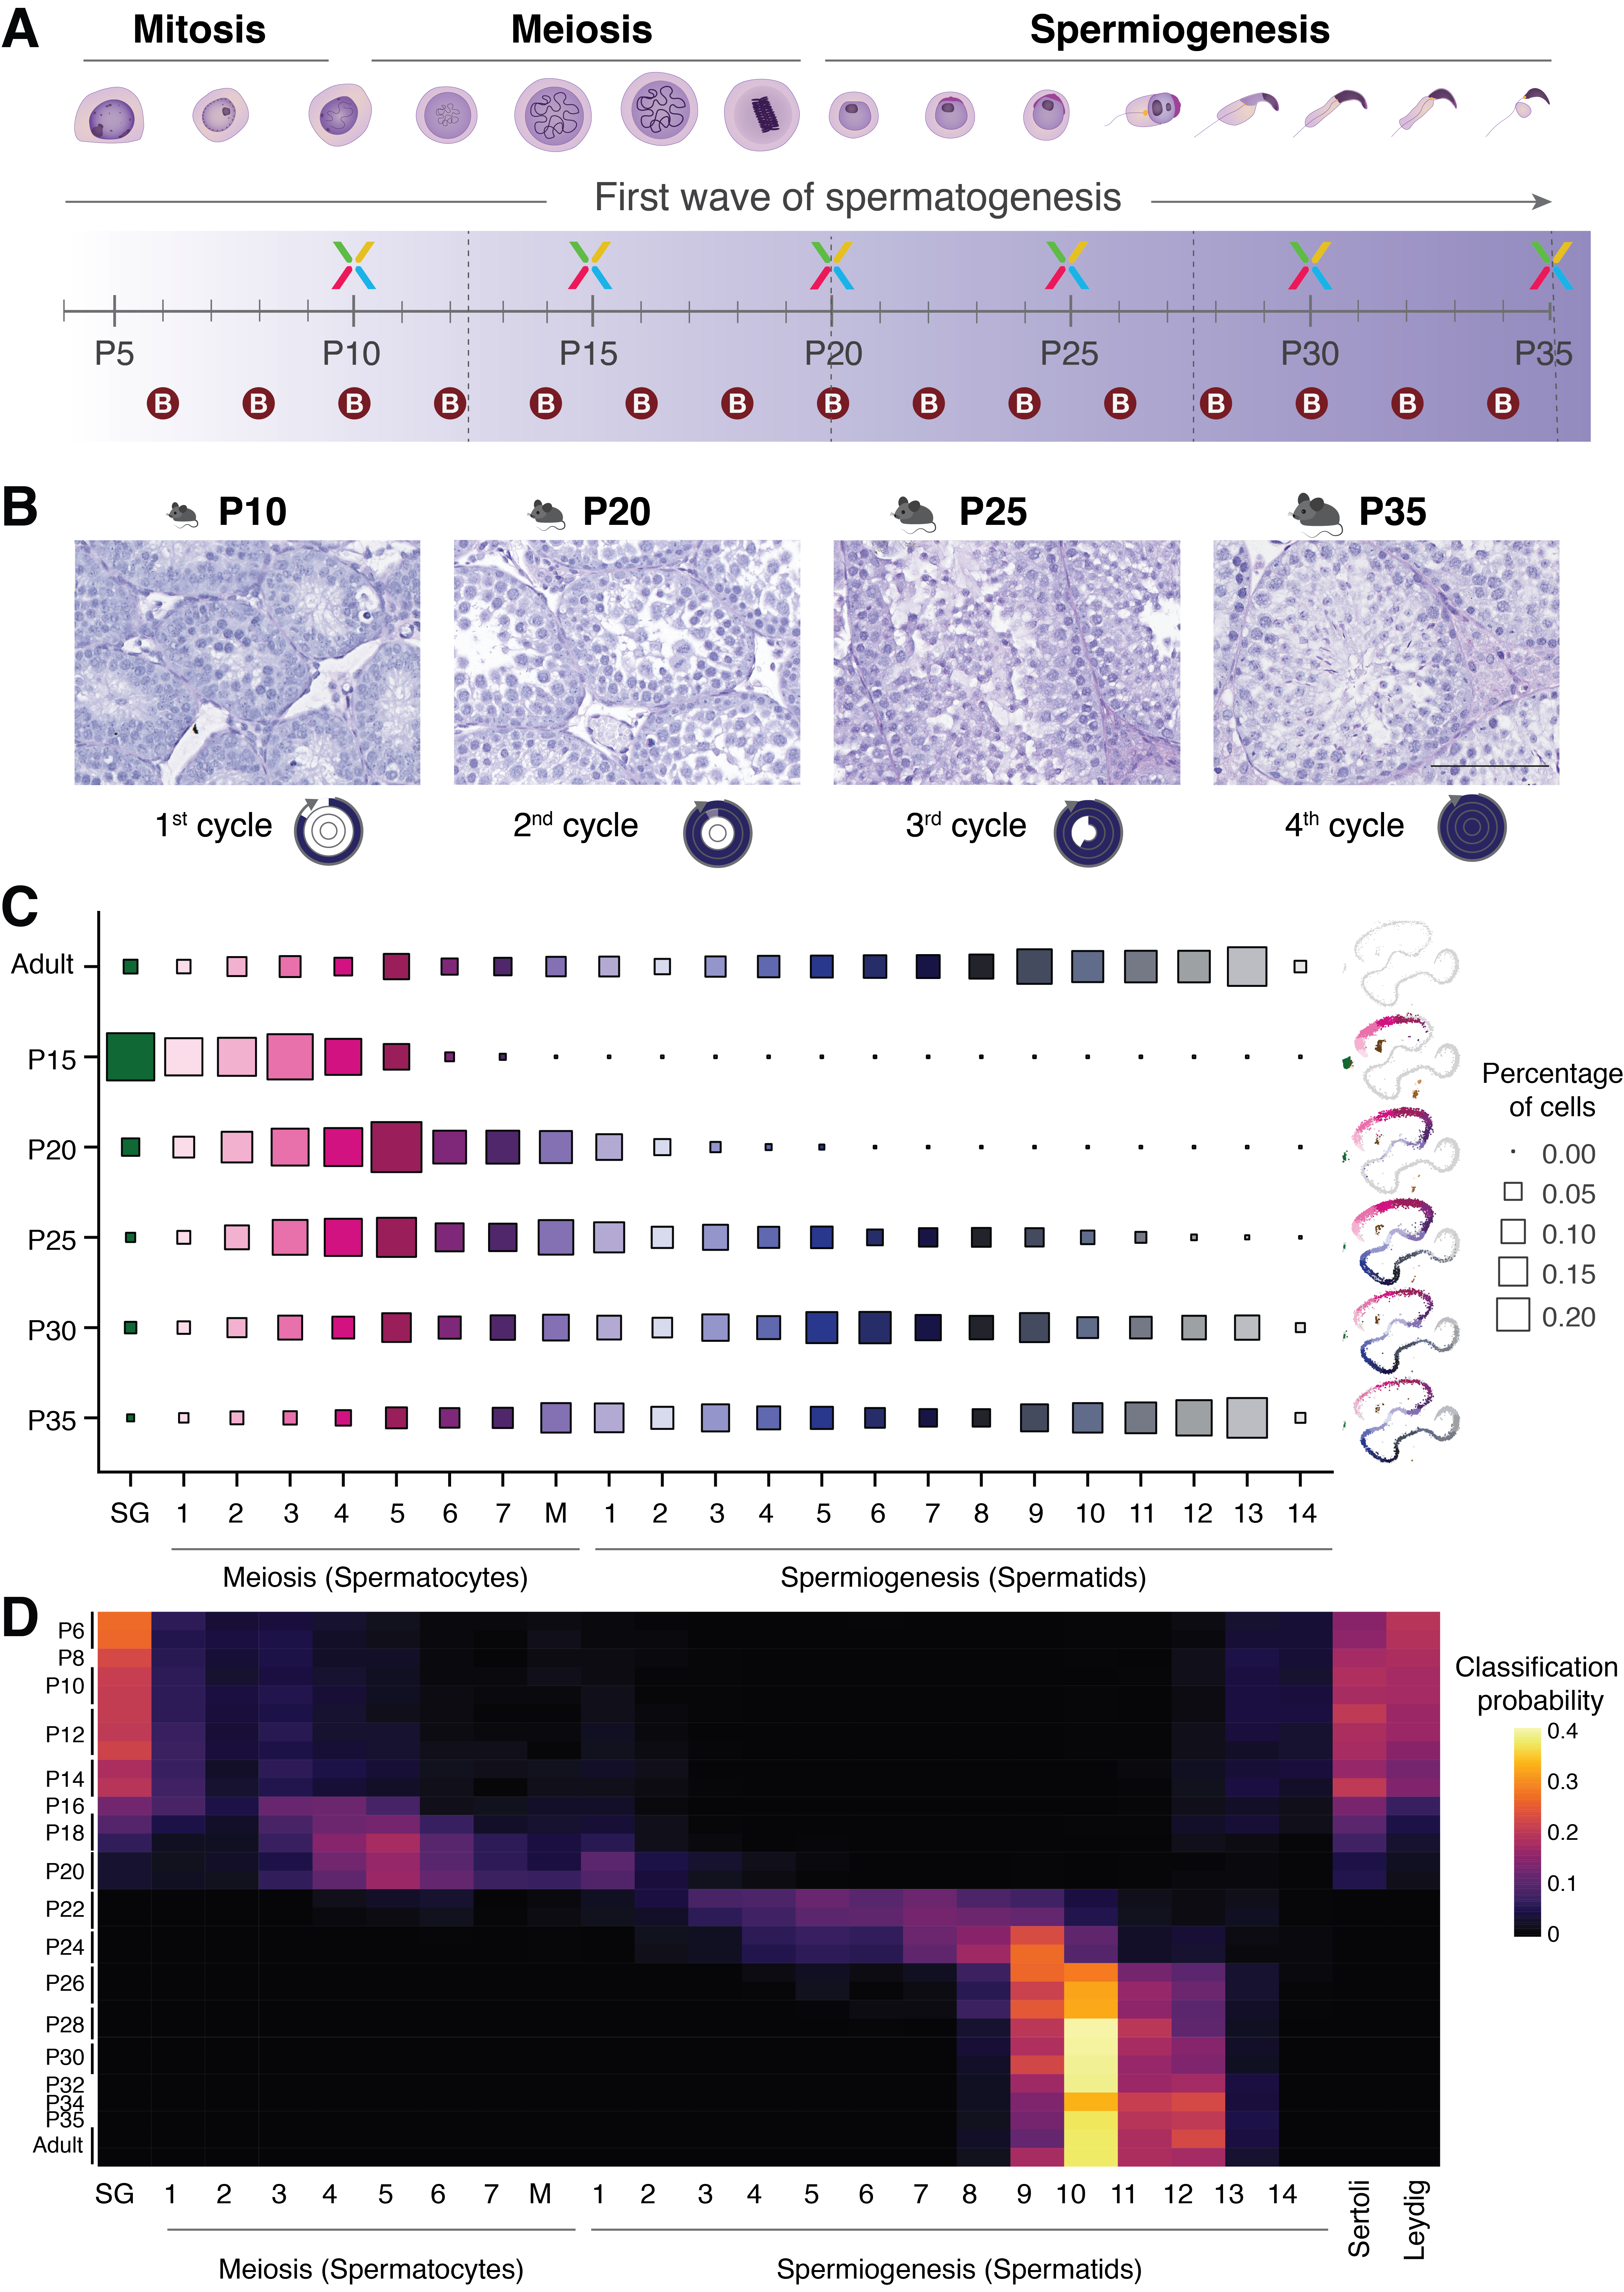
\includegraphics[width=\textwidth]{Fig_4.png}
\caption[Buffering of noise in the colonic crypt]{\textbf{Buffering of noise in the colonic crypt.}\\
Each colonic crypt harbours 6-8 stem cells that divide to form stem cells and progenitors cells. 
Early commitment of progenitor cells to cell fates (e.g.~goblet cells or enterocytes) leads to crypt-to-crypt heterogeneity due to commitment noise (left panel). 
Lateral inhibition within a restricted zone (commitment zone) allows cell fate switching and therefore buffers the crypt-to-crypt heterogeneity (middle panel). 
Migration of goblet cells after the commitment zone buffers the stochastic occurrence of goblet cell or enteroctye patches within the crypt and allows a constant ratio of 1:3 goblet cells to enterocytes in each crypt (right panel). 
Adapted from \citep{Toth2017}.}
\label{fig0:noise_tissue}
\end{figure}

\subsection{Evolution}

As discussed above, biological noise \cor{can be} beneficial for cell fate commitment \cor{but} needs to be \cor{controlled} to allow coordinated expression in cell populations. 
During evolution, a trade-off between cellular plasticity, the expression responsiveness during environmental changes, and robust expression formed. 
Natural selection acts on genetically controlled expansions of quantitative phenotypes, which\cor{, in part, are} derived from biological noise \citep{Eldar2010}. 
For example, \cor{variable} expression of stress response genes allows a cell population to adapt to changing environments \citep{Lopez-Maury2009}. 
Specifically, the expression of genes controlled by TATA-box containing promoters shows strong divergence between species \citep{Tirosh2006}. 
To control for robust expression levels once selection becomes stabilising, noise levels are reduced \citep{Lopez-Maury2009, Eldar2010, Pires2016}. \\

Lehner, 2008 discussed specifically evolutionary selection to minimise noise in genes that show harmful phenotypic effects upon alteration ("dosage-sensitive genes"). 
These genes show low expression \cor{variability} to reduce the probability of altered expression and also lower expression divergence between species \citep{Lehner2008}. 
Furthermore, essential genes tend to cluster in the genome in regions with persistent open chromatin to reduce \cor{the effect of} noise \citep{Batada2007}. 
In line with this, the promoters of core cellular components show a decoupling between expression plasticity and expression \cor{variability}, which indicates that responsiveness in expression is not a general attribute of high expression \cor{variability} \citep{Lehner2010a}. \\

In unicellular populations, \cor{it has been proposed that the contribution of noise on molecular phenotypic variability} evolutionarily increased as a form of rudimentary regulation \citep{Wolf2015}. 
As a consequence, phenotypic heterogeneity increases the adaption rate of cell populations to extreme environments \cite{Bodi2017}. 
Conversely, in multicellular organisms, collections of cells need to respond in a coordinated manner. 
It has therefore been proposed that nuclear compartmentalisation in higher organisms reduces noise by mRNA retention at the nuclear membrane \citep{Battich2013, Stoeger2016}.

\cor{In most cases, cells in an unperturbed state have been profiled to decipher evolutionary selection acting on variability in gene expression.
However, in fluctuating environments where the averaged protein abundance across a cell population is far from the optimum, variability in expression leads to some cells expressing protein levels closer to the optimum. 
By contrast, in stable environments, noise in gene expression can be deleterious by leading to suboptimal growth conditions for many cells\cite{Schmiedel2018,Duveau2018}.
It is therefore crucial to discuss the fitness effect of changes in molecular variability in the context of fluctuating as well as stable environments.}

\subsection{Cancer}

While biological noise \cor{can contributeto } the adjustment of cells to new microenvironments, errors in the form of gene mutations induce transitions from healthy cells towards a cancer attractor state \textbf{(Fig.~\ref{fig0:cancer})} \citep{Marusyk2012}. 
Non-genetic heterogeneity supports the phenotypic adaptation to the new attractor state \citep{Jia2017}. 
The emergence of non-genetic heterogeneity in tumours is coupled to epigenetic dysregulation that allows the survival of cancer cells \citep{Timp2013}. 
Furthermore, it has been proposed that genome wide intra-sample methylation heterogeneity is increased in chronic lymphoitic leukemia increasing cancer cell plasticity in the search for new attractor states \citep{Landau2014}. 
Increased variability in expression can also be observed for more aggressive cancer sub-types across multiple patients \citep{Ecker2015}. \\

An important consequence of \cor{increased} phenotypic heterogeneity in cancer cells is the fractional killing of cell populations upon drug treatment \textbf{(Fig.~\ref{fig0:cancer})} \citep{Flusberg2015}. 
\cor{Variability} in proteins mediating \Gls{TRAIL} induced apoptosis leads to the survival of small fractions of cells \citep{Spencer2009}, which could consequently repopulate the tumour environment. 
Similarly, the stochastic acquisition of DNA damage upon cisplatin exposure introduces heterogeneity in the up-regulation of p53. 
Slow up-regulation leads to cell cycle arrest and inhibits apoptosis while only fast up-regulation leads to cell death \citep{Paek2016}. 
In patient derived melanoma cells, sporadic expression of resistance markers forms a rare cell population that grows into resistant colonies after treatment. 
While pre-resistant cells do not display epigenetic marks and are therefore close to the non-resistant ground state, treatment induces large epigenetic reprogramming, forming stable resistant cancer colonies \citep{Shaffer2017}. 
To tackle this problem, combinatorial therapies have been proposed to reduce variability and fractional killing in cancer cell populations \cite{Paek2016, Roux2015}.\\

\cor{These studies propose a contribution of non-genetic heterogeneity, potentially induced by the loss of noise control, to cancer onset and inefficient treatment response.
However, cancer is a heterogeneous disease that develops in a multi-step process involving disregulation in various cellular systems. 
Therefore, and similar to molecular phenotypic variability in embryonic development, the observed non-genetic heterogeneity can be a phenotypic consequence rather than a driver for cancer onset. }

\begin{figure}[!h]
\centering
\includegraphics[width=\textwidth]{Fig_5.png}
\caption[Heterogeneous cell states and cell responses in cancer development]{\textbf{Heterogeneous cell states and cell responses in cancer development.}\\
Stochasticity in expression introduces non-genetic heterogeneity that supports the adaptation of cancerous cells. 
Cancer progresses to form a collection of cells with divergent expression patterns. 
This phenotypic heterogeneity leads to fractional killing during treatment and cancer recurrence.}
\label{fig0:cancer}
\end{figure}

\newpage

\subsection{Ageing}

Similarly to the onset of cancer, destructive roles of biological noise have been reported during organismal ageing. 
Previously, it has been debated whether expression noise changes during the lifespan of animals \cite{Bahar2006, Warren2007}. 
While these initial studies only used small panels of genes, transcriptional profiling of single cells led to the discovery of a destabilised immune activation programme in CD4\plus{} T cells due to increased expression noise \cite{Martinez-jimenez2017}. 
Similarly, transcriptional noise increases with age in human pancreas coupled to an increased stress signature and atypical hormone expression \citep{Enge2017}. 
For further discussion of age-related effects on transcriptional noise, see \textbf{Chapter 2}. \\


\begin{table}[hb	]
\centering
\caption{Positive and negative effects of biological noise on cellular systems.}
\label{table:effects_noise}
\begin{tabular}{l l l}
\toprule
\toprule
\textbf{System} & \textbf{Friend} & \textbf{Foe} \\ 
\midrule
\midrule
Unicellular organism & Bet-hedging & \\
\midrule
Development and & Probabilistic induction  & \\
differentiation & of cell differentiation & \\
\midrule
Immune response & Plasticity in immune response & \\
 & Control of response strength &   \\
\midrule
Tissue development  & Low cell differentiation rate & Non-uniform development \\ 
and homeostasis &  & Uncontrolled tissue response \\
\midrule
Evolution & Adjustment to  & Non-uniform, stabilising expression \\ 
& fluctuating environment & Uncontrolled tissue responses \\
\midrule
Cancer &  & Phenotypic adaption to cancer state \\
& & Fractional killing of cancer cells \\
\midrule
Ageing &  & Unsynchronised immune response \\
& & Increased stress signatures \\ 
\bottomrule
\bottomrule
\end{tabular}
\end{table}

%!TEX root = ../intro.tex
%******************************
%	 Sources of expression noise
%*****************************

\section{Sources of expression noise} 

\cor{Molecular phenotypic variability} across homogeneous populations of cells \cor{can arise} from intrinsic and extrinsic noise, \cor{and deterministic components} (see \textbf{Box 1} on page \pageref{box1}). 
While intrinsic noise is promoter-specific and therefore induces uncoordinated variation in RNA or protein expression between individual genes, extrinsic noise globally influences gene expression across multiple cells and therefore leads to co-variation across larger sets of genes. 
Here, I give an overview on the different sources of intrinsic and extrinsic noise in a variety of biological systems.

\subsection{Intrinsic noise}

Intrinsic noise in cell populations arises from stochasticity in biochemical reactions that lead to the synthesis of mRNAs (transcription) and proteins (translation) within individual cells. 
Regulatory features on the genomic, epigenetic, transcriptional and translational level influence \cor{and control} the strength of intrinsic noise (for an overview see \textbf{Fig.~\ref{fig0:overview_intrinsic}}).

\begin{figure}[!h]
\centering
\includegraphics[width=0.9\textwidth]{Fig_6.png}
\caption[Regulatory features that modulate expression noise]{\textbf{Regulatory features that modulate expression noise.}\\
Promoter sequence, number of transcription factor (TF) binding sites (TFBS), number of transcriptional start sites (TSS), enhancer elements, RNA polymerase II (RNAPII) loading, DNA methylation, nucleosome positioning, histone modifications, polycomb repressive complex binding, \glspl{miRNA}, nuclear export of mRNA, ribosome binding and blockage via stem loop formation are features that induce gene-specific intrinsic noise.}
\label{fig0:overview_intrinsic}
\end{figure}

\subsubsection{DNA features}

One of the key regulatory steps prior to RNA synthesis is the binding of \glspl{TF} to specific DNA sequences within the regulatory region (promoter) of a gene which then triggers the controlled production of primary RNA transcripts from the DNA of this gene \citep{Latchman1997}. 
Mutations in the DNA sequence such as \glspl{SNV} can alter the binding affinity of TFs and therefore the rate at which a gene is expressed \textbf{(Fig.~\ref{fig0:DNA_features})}. 
A systematic study of the \gls{TDH3} gene expression in yeast found that mutations in known \glspl{TFBS} decrease mean expression and increase expression noise. 
Moreover, Metzger \textit{et al.}, 2015 \cor{proposed} that evolutionary selection removes mutations that increase expression noise and that SNVs with large effects on expression noise show the lowest frequency within sampled yeast strains \citep{Metzger2015}. 
\cor{However, the authors examined one promoter in stable environmental conditions. 
How selection on mutations that induce variability in expression works in more complex systems and across multiple promoters is still unexplored.}\\

One of the most widely studied DNA motifs in relation to transcriptional noise is the TATA-box motif in promoters. 
Generally, TATA-box containing promoters show high levels of transcriptional noise \textbf{(Fig.~\ref{fig0:DNA_features})} \citep{Faure2017}, possibly due to a simple activation cycle containing one or few inactive states \citep{Zoller2015}. 
Moreover, TATA-box containing genes show an increased interspecies variability \citep{Tirosh2006} and higher spontaneous mutational variation \citep{Landry2007}, indicating an increased evolvability of these particular genes. 
In an early study, Raser \textit{et al.}, 2004 studied the noisy expression controlled by the budding yeast \gls{PHO5} promoter. 
This promoter contains the TATA-box motif and it has been shown that transcriptional noise is reduced when a mutational modification decreases the TATA-box strength \citep{Raser2004}. 
A more recent study confirmed this result and found mutations in yeast promoters that eliminate the TATA-box motif which lead to reduced noise levels for these genes \citep{Hornung2012}. 
\cor{The TATA-box is therefore one genomic feature that can differentiate between genes with variable and stable expression and are enriched amongst stress response genes, which support their role in early adjustment to changing environmental conditions \citep{Lopez-Maury2009}.}\\

\cor{However, a} possible confounding factor for the increased noise of TATA-box containing promoters is the number of TFBSs. 
Tirosh \textit{et al.}, 2006 detected a two-fold enrichment of TFBSs in TATA-box containing promoters \citep{Tirosh2006}. 
A later study showed that transcriptional noise scales with increased numbers of TFBSs \textbf{(Fig.~\ref{fig0:DNA_features})} \citep{Sharon2014}. 
Furthermore, TATA-box containing genes lack enhancing histone marks and their increased variability in expression can therefore be explained by repressed chromatin \citep{Choi2008} (see \textbf{Section \ref{sec0:epigenetic}}).  

\begin{figure}[!h]
\centering
\includegraphics[width=0.9\textwidth]{Fig_7.png}
\caption[Features of the DNA sequence induce expression noise]{\textbf{Features of the DNA sequence induce expression noise.}\\
Mutations of the transcription factor (TF) binding site (TFBS), the presence of a TATA box, increase number of TFBSs, reduced number of transcriptional start sites (TSSs) and reduced copy number of genes can induce transcriptional noise.}
\label{fig0:DNA_features}
\end{figure}

Promoters can be classified based on their shape as narrow, with few \glspl{TSS} that predominantly control tissue-specific gene expression, and broad promoters with larger numbers of TSSs that control the expression of house keeping genes. 
Mutations that alter the shape of promoters increase transcriptional \cor{variability} \citep{Schor2017a}. 
Furthermore, promoters with one or few TSS show higher levels of expression variability \textbf{(Fig.~\ref{fig0:DNA_features})} \citep{Faure2017}.

\newpage

In addition to \glspl{SNV}, \glspl{CNV} (usually defined as copy number variability of regions $\geq$ 1kb in comparison to a reference genome) in parts of the genome influence gene expression and contribute to, for example, schizophrenia and autism \citep{Gamazon2015}. 
Combined analysis of DNA and RNA has shown that genes with low copy number tend to be more noisily expressed compared to genes encoded by multiple copies \textbf{(Fig.~\ref{fig0:DNA_features})} \citep{Dey2015}. 
In the context of monoallelic expression, genes located on the X chromosome show increased mRNA half-life which in turn increases transcript stability and reduces noise to levels of autosomal genes \citep{Faure2017}.\\

\cor{In sum, these findings highlight that multiple correlated genomic features are associated with modulating noise. 
It is therefore challenging to disentangle the individual underlying sources of transcriptional variability. }

\subsubsection{Epigenetic factors}
\label{sec0:epigenetic}

Epigenetic research is defined as "the study of changes in gene function that are mitotically and/or meiotically heritable and that do not entail a change in DNA sequence" \citep{Wu2001}. 
Epigenetic factors are generally described as DNA methylation at \gls{CpG} dinucleotides, histone modifications and nucleosome positioning  \citep{Portela2010}. 
\textbf{Table \ref{tab0:epigenetic}} summarises the relationship between epigenetic features and \cor{variable} gene expression. \\

\Gls{CGI} are genomic sites of more than 200 bases with a GC content of more than 50\% and are usually unmethylated. 
Methylation of CGIs in promoters is linked to gene silencing while DNA methylation in gene bodies facilitates transcription \citep{Portela2010}.  
Recently, the presence of CGIs in gene bodies but also at the TSS and in promoter regions was linked to a reduction in transcriptional \cor{variability} \citep{Faure2017}. 
\cor{Morgan and Marioni, 2018 further distinguished between gene promoters associated with short and long CGIs.  
Similar to the presence of TATA-box motifs as described above, the length of CGIs in promoter regions controls how variably a gene is expressed. 
Genes associated with short CGIs tend to be more variably expressed and allow an early response to stimulation, exemplified by observations in mouse bone-marrow derived dendritic cells and human breast cancer cells \citep{Morgan2018}.
However, it is not clear whether the length of CGIs is the sole driver for variable gene expression or how multiple genomic features work together to induce transcriptional variability.} \\

Modifications of histones induce the \cor{opening} or repression of chromatin and  therefore indirectly modulate gene expression \citep{Suganuma2011}. 
In an extensive study to link histone modifications to transcriptional \cor{variability}, Faure \textit{et al.}, 2017 detected several histone modifications in promoter/core promoter motifs, at the TSS and in gene bodies that increase or decrease \cor{variability}. 
The repressive \gls{H3K27me3} mark is linked to higher \cor{variability} when present at the TSS, in promoters and in gene bodies. 
The enhancer related \gls{H3K4me1} mark only increases \cor{variability} when present at the TSS and in the core promoter sequence while the repressive \gls{H3K9me3} mark increases \cor{variability} when present in the promoter motif. 
The activating marks \gls{H3K4me3}, \gls{H3K9ac} and \gls{H3K36me3} are linked to low levels of \cor{variability} when present in gene bodies. 
In addition to these single features, bivalent promoters that carry the repressive \gls{H3K27me3} and enhancing \gls{H3K4me3} marks show high levels of transcriptional \cor{variability} \citep{Faure2017}.
\cor{Here and in Morgan and Marioni, 2018, the authors profiled molecular phenotypic variability in "homogeneous" populations of \glspl{mESC} as proxy for transcriptional noise.
While the effect of fluctuation in cell-cycle stages was regressed out, unobserved variation in, for example, the differentiation potential of mESCs in serum grown medium \cite{Kolodziejczyk2015cell} could still exist.
It is therefore difficult to use scRNA-Seq data to study the true underlying effect of transcriptional noise on the overall observable phenotypic variability.}\\ 

\cor{One suggestion why bivalent promoters show high transcriptional variability was brought forward by Kar \emph{et al.}, 2017.
Here, the authors studied the function of \glspl{PRC} in mESCs.}
PRCs are epigenetic modifiers of histones that repress transcription of developmental genes \citep{Chittock2017} and they can bind together with active \gls{RNAPII} to bivalent promoters. 
Switching between the repressed and active states introduces gene expression variability across a population of cells \cite{Kar2017}.
\cor{However, bulk measures were used to identify the bivalency of promoters.
That leaves the possibility that in a fraction of cells the promoter resides in an open state while in other cells the promoter is repressed. 
This highlights the fact that bulk measures might not be suitable to obtain a correct measure of promoter states in cell populations that could contain unobserved cell state heterogeneity.} \\

Chromatin is the packaged state of DNA within the nucleus and its central elements are nucleosomes. 
Nucleosomes are combinations of eight of the four histones (H3, H4, H2A, H2B) around which 147 bases of DNA twist. 
An array of histone modifying enzymes exist that regulate the opening or closing of the chromatin; termed heterochromatin and euchromatin, respectively \citep{Kouzarides2007}. 
Tirosh \textit{et al.}, 2008 showed that promoters with high nucleosome occupancy close to the TSS tend to display a high range of expression levels across varying conditions (transcriptional plasticity). 
Distant nucleosome-rich regions are on the other hand associated with low transcriptional \cor{variability} \citep{Tirosh2008}. 
Nucleosome covered promoters display shorter transcriptional rates, which in turn explains increased transcriptional \cor{variability} for these promoters \cite{Dey2015}. 
Single-cell measures indicate cell-to-cell variations in nucleosome positioning around the \textit{PHO5} promoter upon stress induction. 
Even in the non-stressed state, a small fraction of cells exhibit nucleosome free regions at the promoter which explains low and possibly noisy expression of \textit{PHO5} \citep{Small2014}.
\cor{This observation again highlights the lack of resolution when using bulk measures to profile the promoter architectures in cell populations.
However, current single-cell technologies to profile epigenetic marks lack throughput and are influenced by high levels of technical noise.
The observed variations in nucleosome occupancy could therefore be driven by technical variation.} \\

Boundaries between heterochromatin and euchromatin are controlled by boundary elements, such as the transcription factor \Gls{CTCF}, that recruit chromatin modifying factors \citep{Kouzarides2007}. 
CTCF also regulates transcription by activating or repressing promoters and regulates distant chromatin interactions \citep{Kim2015a}. 
Recent studies suggest that long-range enhancer-promoter interactions modulate transcriptional noise. 
Interference of CTCF-mediated enhancer-promoter contact either by CTCF knock-out or CTCF-binding site deletion leads to increased expression variability in selected genes \citep{Ren2017}. 
\cor{This study however only profiled protein abundance of few genes and did not correct for changes in mean expression that are highly correlated with changes in variance \cite{Brennecke2013}.}
Enhancers are cis-regulatory elements of non-coding DNA containing TFBSs that regulate the expression of neighbouring genes \citep{Blackwood1998}. 
Genes within super-enhancer loci, a region with multiple enhancers, control pluripotency master regulators and show high levels of variability in expression down-stream targets of these master regulators show similar co-variation across mESCs \citep{Faure2017}.

\newpage

\begin{table}[hb	]
\centering
\caption{Epigenetic control of transcriptional noise}
\label{tab0:epigenetic}
\begin{tabular}{l l c c}
\toprule
\toprule
 & Feature & \cor{Variable} & Stable \\ 
\midrule
\midrule
\multirow{3}{*}[-2pt]{DNA methylation} & CGIs &  & \checkmark{} \\
\cmidrule{2-4}
& Short CGIs & \checkmark{} &  \\
\cmidrule{2-4}
& Gene body methylation &  & \checkmark{} \\
\midrule
\multirow{7}{*}[-2pt]{Histone modification} & H3K27me3 (TSS, promoter, gene body) & \checkmark{}  & \\
\cmidrule{2-4}
& H3K4me1 (TSS, promoter) & \checkmark{}  & \\
\cmidrule{2-4}
& H3K9me3 (promoter) & \checkmark{}  & \\
\cmidrule{2-4}
& H3K4me3 (gene bodies) &  & \checkmark{}\\
\cmidrule{2-4}
& H3K9ac (gene bodies) &  & \checkmark{} \\
\cmidrule{2-4}
& H3K36me3 (gene bodies) &  & \checkmark{} \\
\cmidrule{2-4}
& H3K27me3 and H3K4me3 & \checkmark{}  & \\
\midrule
\multirow{3}{*}[-2pt]{Nucleosome position} & Nucleosome rich promoters & \checkmark{} & \\
\cmidrule{2-4}
& Distant nucleosome rich regions &  & \checkmark{} \\
\cmidrule{2-4}
& Deletion of nucleosome remodelling complexes & \checkmark{}  & \\
\midrule
\multirow{7}{*}[-2pt]{Genome architecture} & CTCF knock-out & \checkmark{} & \\
\cmidrule{2-4}
& CTCF binding site depletion & \checkmark{} & \\
\cmidrule{2-4}
& Clustered genes &  & \checkmark{} \\
\cmidrule{2-4}
& Nuclear-lamina associated genes & \checkmark{} & \\
\bottomrule
\bottomrule
\end{tabular}
\end{table} 

Moreover, the positioning of genes on the genome controls expression noise with densely clustered genes being less \cor{variably} expressed in comparison to non-clustered genes \citep{Kustatscher2017}. 
Additionally, genes positioned next to “noisy” genes display higher levels of transcriptional variability compared to genes that are located in proximity to “stable” genes \citep{Kar2017}. 
Expression \cor{variability} is also increased for genes that are located in a repressed neighbourhood, namely active genes in constitutive nuclear lamina-associated domains \citep{Faure2017}.
\cor{This finding again highlights that genes associated with repressed chromatin display higher transcriptional variability compared to genes associated with open chromatin.
Single-cell measures are needed to provide an insight into whether this effect is driven by so called "leaky" expression from closed promoters of if heterogeneous promoter states can be observed.}

\subsubsection{Transcriptional features}

Transcription is initiated by TFs binding to specific regulatory DNA sequences followed by recruitment of RNAPII and RNA synthesis. 
As discussed above, promoter architecture, namely the location and accessibility of TFBS and RNAPII binding sites, dictates mean expression and transcriptional \cor{variability}. \\

In bacteria, the intracellular physical distance between TF source and the promoter sequence influences expression variability. 
TF expression proximal to their target genes results in less \cor{variable} expression compared to TF expression which occurs distant to the promoter sequence \citep{Goni-Moreno2017}. 
Once TFs bind to their target sequence, Carey \emph{et al.}, 2013 showed that the mean expression to \cor{expression variability} ratio is promoter dependent while in the majority of cases, \cor{variability} negatively scales with mean expression \citep{Carey2013}. \\

Similar to TF binding dynamics, the assembly of RNAPII complexes modulates transcriptional noise. 
An early study identified the connection between paused RNAPII and synchronous expression of target genes. 
Genes without pre-loaded RNAPII show more stochastic activation patterns \citep{Boettiger2009}. 
This finding has later been confirmed using scRNA-Seq data where increased variability was detected for genes with actively transcribing RNAPII across the full range of expression levels \textbf{(Fig.~\ref{fig0:RNAPII})} \citep{Day2016}.
\cor{However, genes with pre-loaded RNAPII also have a higher CpG content and are depleted for TATA-box elements \cite{Day2016}. 
Once again, the correlation between genomic factors and their individual associations with variation creates a challenge for disentangling their specific effects on molecular phenotypic variation.
Alternatively, this may also represent multiple regulatory layers that combine to modulate noise. }\\

\begin{figure}[!h]
\centering
\includegraphics[width=0.7\textwidth]{Fig_8.png}
\caption[RNAPII pausing reduces transcriptional noise]{\textbf{RNAPII pausing reduces transcriptional noise.}\\
Left: Pre-loaded RNA polymerase II (RNAPII) allows direct transcription upon transcription factor (TF) binding. 
Right: RNAPII recruitment induces gene expression variability.}
\label{fig0:RNAPII}
\end{figure} 

\newpage

\subsubsection{Post-transcriptional and translational features}

After synthesis, pre-RNAs are polyadenylated and spliced to form mRNA that relocates from the nucleus to the cytoplasm where translation occurs to synthesise proteins \cite{Glisovic2008}. 
On the post-transcriptional and translational level, mRNA location, structure, degradation and translation have been shown to influence cell-to-cell variation in protein abundance.\\

Upon transcriptional activation, RNAs are produced in burst-like patterns where burst frequency modulates mean expression and noise, and burst size influences solely mean expression \citep{Hornung2012}. 
While bursty transcript synthesis introduces stochastic fluctuations in nuclei between cells, active export of mRNAs into the cytoplasm can dampen this source of variability \textbf{(Fig.~\ref{fig0:posttranscriptional})} \citep{Battich2015a}. 
Reduced cytoplasmic noise has also been shown for two nuclear-retained genes in the mammalian liver. 
Furthermore, this mode of noise control was proposed to be active across a range of metabolic tissues \cite{BaharHalpern2015a}.

\begin{figure}[!h]
\centering
\includegraphics[width=\textwidth]{Fig_9.png}
\caption[Post-transcriptional regulation to control noisy expression]{\textbf{Post-transcriptional regulation to control noisy expression.}\\
Bursty expression introduces nuclear variation in transcript abundance that is buffered due to retention at the nuclear membrane. Within the cytoplasm, micro RNAs degrade lowly expressed genes to reduce expression noise. 
Deletion of the ribsosome binding site as well as stem loop formation increase variability in protein abundance across cells. 
Arrows indicate either increased (red) or decreased noise (green) depending on the regulatory mechanism.}
\label{fig0:posttranscriptional}
\end{figure} 

\cor{Conversely, a recent study by Hansen \emph{et al.}, 2018 proposed an amplification of transcriptional variability due to nuclear export \cite{Hansen2018}. 
However, the authors computed the Fano factor (variance divided by mean expression) as measure of variability and assumed that its value is not correlated with mean expression. 
This assumption arises from an underlying Poissonian (Fano factor is equal to 1) or over-dispersed Poissonian (Fanor factor is larger than 1) distribution of transcript counts.
In reality, the Fano factor is not constant across the range of mean expression. 
This has been discussed by Gr\"un \emph{et al.}, 2014, who showed scale differences in the coefficient of variation (CV) versus mean expression dependency for lowly and highly expressed genes \cite{Grun2014}.
Hansen \emph{et al.} also showed this effect when plotting the Fano factor versus mean expression.
Across all genes, the cytoplasmic transcript abundance as well as the Fano factor were larger compared to nuclear measures, which is to be expected by the model proposed by Gr\"un \emph{et al.}, 2014.
It is therefore recommended to fit a non-parametric curve to variability measure versus mean expression and compare the regression residuals as explained in Chapter 3.}\\

Within the cytoplasm, mRNAs are subject to translation or degradation. 
At this stage, \cor{variability induced by} bursty gene expression is propagated to form variation in protein abundance. 
The availability of mRNAs for translation is not only dictated by their synthesis but also their degradation rate. 
mRNA degradation is accelerated by recognition of \glspl{miRNA}. 
This process has been shown to preferentially reduce noise levels for lowly expressed genes in mESCs, possibly to retain cellular identity \textbf{(Fig.~\ref{fig0:posttranscriptional})} \citep{Schmiedel2015}. 
\\

In addition to noise introduced by stochastic processes on the transcriptional level, the recognition and binding of ribosomes to mRNAs for translation initiation is a source for variation in protein abundance. 
Modulating translational efficiency by mutating the ribosome binding site and initiation codon showed an association between translation and variation in protein abundance \textbf{(Fig.~\ref{fig0:posttranscriptional})} \citep{Ozbudak2002}. 
Additionally, mRNA secondary structure formed by stem loops and poly(G) motifs affects translation initiation and increases variation in protein levels \textbf{(Fig.~\ref{fig0:posttranscriptional})} \citep{Dacheux2017a}.\\

\cor{Together, these studies again highlight a multitude of factors that can modulate the observable variation in transcript and protein abundance. 
Moving forward, models that correct or account for variations introduced by different factors need to be developed to disentangle the individual sources of molecular variation.}

\newpage

\subsection{Extrinsic noise}

\cor{Classically, extrinsic noise has been described to arise from fluctuations in molecules that affect the global gene expression landscape of the cell \cite{Elowitz2002}.
Measuring extrinsic noise is only possible in bacterial populations that do not show fluctuations in cell states.
Nowadays, extrinsic noise is often described to arises from cells being in different regulatory states.}
Here, differences in cellular components introduce variation in mRNA and protein abundance. 
The presence of cell states in otherwise homogeneous populations is characterised by differences in metabolism, cell cycle, cellular volume, cell-to-cell and environmental signalling as well as cell density. 
It has been shown that extrinsic noise forms a major contribution to variation in gene expression and that transcript distributions can be predicted from the cellular state, population context and microenvironment \citep{Battich2015a}.
\cor{Being able to predict transcript abundance however indicates that extrinsic noise is not purely stochastic but might also contain deterministic components.}

\begin{figure}[!h]
\centering
\includegraphics[width=0.7\textwidth]{Fig_10.png}
\caption[Differences in cell states induce extrinsic noise]{\textbf{Differences in cell states induce extrinsic noise.}\\
Within a homogeneous population of cells (left), individual cells reside in different cellular states (e.g.~cell cycle, cell signalling, metabolism) and show differences in cellular volume.}
\label{fig0:extrinsic}
\end{figure} 

\subsubsection{Cell cycle}

Cell cycle has been widely discussed to form a \cor{major} source of extrinsic noise \citep{Colman-Lerner2005, Newman2006}. 
In yeast populations, differences in transcriptional activities between the G1 and S/G2/M phases of the cell cycle lead to large-scale transcriptional heterogeneity across cell populations \textbf{(Fig.~\ref{fig0:extrinsic})} \citep{Zopf2013}. 
Under nutrient-poor conditions, growth rate is reduced and \cor{transcriptional variability} is elevated due to cells being in different cell cycle stages \citep{Keren2015}. 
Even under optimal growth conditions for mESCs (2i media), cell cycle related genes show strong heterogeneity in expression across the cell population \citep{Kolodziejczyk2015cell}. 
\cor{However, it is possible that unobserved regulatory mechanisms are in place to induce proliferation, which otherwise appears to occur randomly across a population of cells.}
When quantifying cell-to-cell variation, cell cycle induced extrinsic noise is often seen as unwanted variation and can mask more subtle transcriptional heterogeneity. 
Computational methods have been developed to correct for this confounding effect to enhance the underlying signal \citep{Buettner2015, Buettner2017}. 

\subsubsection{Cell volume}

Cellular volume provides another explanation for global differences in mRNA content between individual cells introducing large-scale transcriptional \cor{variability} \textbf{(Fig.~\ref{fig0:extrinsic})}. 
Even though cell volume changes during cell cycle progression, within each phase, cell volume can vary as much as across all phases. 
It has been shown that mRNA counts scale with cellular volume to maintain transcript concentrations within each cell \citep{Kempe2015, Padovan-Merhar2015, Zhurinsky2010}. 
\cor{Again, it is not fully understood how cell volume is controlled across a population of cells; especially within multicellular organisms. 
Therefore, the volume of a cell does not necessarily stochastically but rather deterministically contribute to the observed molecular phenotypic variability.}
To avoid this source of heterogeneity, normalisation approaches correct for differences in mRNA content between individual cells \citep{Vallejos2017}.

\subsubsection{Metabolism}

The effect of metabolic fluctuations has been studied in \textit{E. coli} populations. 
Variations in biochemical reactions are induced by noise in the expression of their corresponding catalytic enzymes. 
Changes in metabolism are then coupled to varying growth rates of individual cells, which in turn introduce large-scale transcriptional heterogeneity in cell populations \textbf{(Fig.~\ref{fig0:extrinsic})} \citep{Kiviet2014}.  

\subsubsection{Expression capacity}

Expression capacity is defined as the ability of a cell to express proteins from a gene by utilising the transcriptional and translational machinery. 
Fluctuations in the expression capacity of cells due to quantitative differences in RNAPII or ribosomes can induce global variability among the majority of proteins \citep{Colman-Lerner2005}.

\newpage

\subsubsection{Cell signalling}

A different source of extrinsic noise is the intra- or inter-cellular signalling state of individual cells. 
Fluctuations in membrane bound or cytoplasmic proteins lead to inconsistent transmission of signalling stimuli as exemplified by variability in \gls{TRAIL}-induced apoptosis \citep{Spencer2009}. 
Similarly, variations of regulators in the \gls{ERK} signalling pathway introduce downstream variability in nuclear response \textbf{(Fig.~\ref{fig0:extrinsic})}. 
The degree to which nuclear ERK response varies depends on the position of the regulator in the topology of the signalling pathway \citep{Iwamoto2016}. 
In \textit{C. elegans}, perturbation of the Wnt signalling pathway displayed different degrees of variability in expression of the key Hox gene for Q neuroblast migration, \textit{mab-5}. 
It has been proposed that extrinsic noise, in this case the strength of the Wnt signal, modulates intrinsic variation in the expression of \textit{mab-5} \citep{Ji2013}. 
\cor{These examples describe a system where noise introduces variation in individual components. 
However, this variation is modulated by signalling networks, which allows the cells to precisely respond to external cues. }

\subsubsection{Physical constraints}

\begin{wrapfigure}{r}{0.5\textwidth}
\centering    
\includegraphics[width=0.48\textwidth]{Fig_11.png}
\caption[Physical constraints induce heterogeneous expression patterns.]{\textbf{Physical constraints induce heterogeneous expression patterns.} \\
Cell density increases during the expansion of a homogeneous population of cell forming patches with high and low density, pushing cells to the edge of the population. 
Based on these physical constraints, cells change their transcriptional programme, inducing variability across the population.}
\label{fig0:constrains}
\end{wrapfigure}

Physical constraints on cell growth and the direct population context influence the state of individual cells \citep{Battich2015a}. 
Snijder \textit{et al.}, 2009 performed detailed imaging based analysis of adherent human cells that were infected with different viruses. 
Clathrin mediated endocytosis was most variable with low cell density leading to inefficient mouse hepatits virus infection. 
Dengue virus preferentially infects edge cells while simian virus 40 infection decreased with large cell density \citep{Snijder2009}. 
These experiments indicate the importance of local cellular microenvironment and cell-cell contacts leading to heterogeneity in cell states \textbf{(Fig.~\ref{fig0:constrains})}. 


%!TEX root = ../intro.tex
%******************************
%	 Quantification of biological noise
%*****************************

\section{Quantification of cell population heterogeneity} 

\cor{In the last ten years, the scale of single-cell assays increased from measuring few to hundreds and thousands of genomic, epigenetic, transcriptomic or proteomic features. These technologies can be used to measure molecular phenotypic variability, as well as gain an understanding of the regulatory features that modulate it. The ability to study noise using technology that destroys the cell is formulated on the basis that a cross-section over a population of cells is representative of the time-resolve noise profile of any given cell\cite{Ozbudak2002}.} 
In this section, I will discuss the applicability of single-cell sequencing and imaging technologies as a potential read-out for cell population heterogeneity induced by transcriptional noise.

\subsection{Single-cell sequencing}

Next generation sequencing approaches have been applied to individual cells to quantify variation in DNA sequence, mRNA expression, epigenetic marks and protein abundance within a cell population. 

\subsubsection{Single-cell whole genome sequencing}

\Gls{scDNA-Seq} has previously been used to identify CNVs and SNVs between single cells \citep{Zong2012}. 
Based on these read-outs, tumour heterogeneity and evolution \citep{Navin2011} as well as lineage relationships in the human brain were inferred \citep{Evrony2015}. 
To obtain enough genomic material, \gls{WGA} is performed on DNA from individual cells. The \gls{SCOMP} degrades DNA via restriction enzymes, includes a primary \gls{PCR} amplification step and a later re-amplification via comparative genomic hybridisation \citep{Klein1999}. \Gls{MDA} is based on the random initiation of amplification via oligonucleotide primers with strand displacement \citep{Dean2002}. Compared to MDA, \gls{MALBAC} achieves an initial quasi-linear amplification step by pre-amplification using primers with handle sequences. 
Full amplicons form hairpins that are exponentially amplified prior to sequencing \citep{Zong2012}. \\

The main limitation of single-cell DNA sequencing is the genomic coverage per cell. 
While the detection of SNVs requires deep sequencing of individual cells, CNVs can be detected with shallow sequencing therefore allowing the throughput to increase \textbf{(Fig.~\ref{fig0:scDNA-Seq})} \citep{Knouse2016, Baslan2015}. 
Recently, Vitak \emph{et al.}, 2017 introduced \gls{sci-Seq} which allows the generation of thousands of single-cell genomes for sequencing. 
In the first step, multiple nuclei are sorted into each well of a 96 well plate and the genomic DNA is labelled with barcodes by transposase tagging. 
In the second step, 15-25 tagged cells are sorted into individual wells of a PCR plate where the second round of barcoding is performed during amplification. In that way, CNVs of over 15,000 cells can be assessed \citep{Vitak2017}.
\cor{While previously only bulk measures have been used to link mutations to changes in transcriptional variations\cite{Metzger2015}, scDNA-Seq with high read-depth can be used to solve the question of whether the same mutation in each cell (germ line mutation) or a heterogeneous mutational pattern (somatic mutation) causes the observed increase/decrease in phenotypic variability.}

\begin{figure}[!h]
\centering
\includegraphics[width=\textwidth]{Fig_12.png}
\caption[ScDNA-Seq allows detection of SNVs and CNVs between individual cells]{\textbf{ScDNA-Seq allows detection of SNVs and CNVs between individual cells.}\\
Individual nuclei are captured in 96-well plates and directly lysed or fixated for multiplexing. Whole genome amplification (WGA) can be performed using MDA, MALBAC or SCOMP resulting in amplified genome segments. 
Depending on the biological question, whole genomes are either sequenced thoroughly to detect single nucleotide variants (SNVs) while shallow sequencing can be used to detect copy number variations (CNVs).}
\label{fig0:scDNA-Seq}
\end{figure}

\vspace{-5mm}

\subsubsection{Single-cell RNA sequencing}

Initial approaches to quantify mRNA abundance within single cells included targeted microfluidic-based single-cell \gls{RT-PCR} \citep{Warren2006} and whole-transcriptome read-outs of hand-picked cells \citep{Tang2009}. 
Methods for cell capture range from micromanipulation \citep{Grindberg2014} and laser capture microdissection \citep{Frumkin2008} as targeted methods with low throughput to  \gls{FACS} \citep{Hayashi2010, Dalerba2011, Jaitin2014}, microfluidics \citep{Trapnell2014, Treutlein2014} and microdroplets \citep{Klein2015, Macosko2015} as high-throughput approaches \textbf{(Fig.~\ref{fig0:scRNA-Seq})}. 
More broadly, microfluidic-based \gls{scRNA-Seq} approaches can be grouped into valve-, droplet- or well-based strategies \citep{Prakadan2017}. \\

A variety of scRNA-Seq protocols have been published that utilise different methods for mRNA \gls{RT}, \gls{cDNA} amplification and library preparation. 
All of these commonly used techniques for scRNA-Seq select and reverse transcribe mRNA (poly(A) tailing). 
The initial protocol introduced by Tang \textit{et al}, 2009 \citep{Tang2009} was improved by incorporating a template switching mechanism at the 5' end of the mRNA thus reducing the 3' sequencing bias present in previous methods \citep{Islam2011} (see below and \textbf{Fig.~\ref{fig0:scRNA-Seq}}). 
This \gls{STRT} method shows 5' bias in read mapping and was later modified for full-length transcript detection (SmartSeq \citep{Ramskold2012} and SmartSeq2 \citep{Picelli2013}). 
CEL-Seq \citep{Hashimshony2012} and CEL-Seq2 \citep{Hashimshony2016} use \gls{IVT} to linearly amplify cDNA prior to sequencing as opposed to exponential amplification in other techniques. 
Protocols for sequencing library preparation have been optimised for Illumina, SOLiD or PacBio sequencing \citep{Kolodziejczyk2015review}. \\

During scRNA-Seq, minute amounts of mRNA are captured and amplified generating a high degree of technical noise, which distorts quantification of true biological variability. 
To account for this, a set of external RNAs developed by the \gls{ERCC} \citep{Rna2005} can be added to the cell lysate. 
Based on the reads mapped to ERCC spike-ins, technical noise can be removed from total expression variability \citep{Brennecke2013, Vallejos2015BASiCS}. 
Another way to reduce noise derived from amplification biases in scRNA-Seq experiments is to tag each mRNA molecule with a \gls{UMI} \citep{Kivioja2011, Islam2014}.\\

One example of a commercially available platform that captures individual cells and performs lysis, reverse transcription and pre-amplification of cDNA is the Fluidigm\textsuperscript{\textregistered{}} C1 system. 
Individual cells are loaded into \glspl{IFC}, also termed "chips", that allows capturing of 96 to 800 cells. 
Depending on the size of the cells, this system offers chips with different capture well sizes. 
Each well can be microscopically inspected to differentiate between empty capture sites and single cells \citep{Kolodziejczyk2015review}. 
The C1 system uses the SMARTer\textsuperscript{\textregistered{}} chemistry to capture poly(A) mRNA with modified oligo(dT) primer. 
Next, the \gls{RTase} reverse transcribes from the 3' to the 5' end of the mRNA and adds non-templated deoxycytidines to the 3' end of the cDNA. The template-switch primer contains guanosines at its 3' end that base-pair with the deoxycytidines on the cDNA to create an extended template. 
The \gls{RTase} extends to the end of the template-switch primer. 
This produces single-stranded cDNA that contains the SMARTer tag sequence, the 3' end of the mRNA, the full-length transcript up to the 5' end of the mRNA, and the reverse complement of the SMARTer tag sequence. 
Amplification of this cDNA is performed by PCR on the chip \cite{Fluidigm2015}. After pre-amplification, the cDNA is collected and prepared for sequencing.\\

In parallel to extending scRNA-Seq protocols to robustly capture mRNA transcripts, efforts have been made to increase the throughput of this technology. 
Jaitin \emph{et al.}, 2014 introduced \gls{MARS-Seq} to sequence over 4000 cells of the mouse spleen. 
MARS-Seq captures cells in 384 well plates and labels transcripts of each cell with a combination of 2 random barcodes. 
This multiplexing strategy is performed using a liquid handling robot and cells can be pooled for sequencing library preparation which reduces costs and time effort \citep{Jaitin2014}. 
The first large-scale technique that captured tens of thousands of cells was introduced by Fan \emph{et al.} in 2015. 
Here, 10,000 cells were captured in a 100,000 microwell surface. 
Additionally, barcoded beads were loaded into the surface until saturation. 
This Cyto-Seq approach is similar to the more recent Seq-Well technology \citep{Gierahn2017}. 
Each bead is coated with barcodes containing a unique sequence, a bead-specific barcode, a UMI and a oligo(dT) primer. After cell lysis and mRNA capture, beads are pooled and cDNA synthesis can be performed prior to sequencing \citep{Fan2015}. 
In the same year, the inDrop and Drop-Seq technologies were introduced \citep{Klein2015, Macosko2015}. 
Both technologies use microfluidic platforms to merge droplets containing barcodes, lysis and reverse transcription reagents with droplets containing cells. 
Similar to the above described Cyto-Seq \citep{Fan2015}, after lysis and mRNA capture, droplets are pooled for sequencing. 
The main difference is that cell-specific barcodes in Drop-Seq are bound to beads and to a polyacrylamide mesh in inDrop.  

\begin{figure}[!h]
\centering
\includegraphics[width=0.9\textwidth]{Fig_13.png}
\caption[Workflow for scRNA-Seq technologies]{\textbf{Workflow for scRNA-Seq technologies.}\\
Single cell suspensions are obtained by tissue dissection and dissociation. 
Commonly used cell capture technologies include fluorescence-activated cell sorting (FACS), valve-based microfluidics (Fluidigm\textsuperscript{\textregistered{}} C1 system), droplet-based microfluidics (10X Genomics\textsuperscript{\textregistered{}} system), or picowells. 
After cell capture and lysis, poly(dT) oligos capture mRNA prior to reverse transcription. 
In the case of droplet-based cell capture, poly(dT) oligos are tagged with a unique molecular identifier (UMI) and a cell-specific barcode. 
\Gls{RT} generates cDNA from the template RNA. One strategy for RT is the template-switching protocol where the reverse transcriptase adds three cytidines at the 5' end of the template. 
A \gls{TSO} binds to the cytidines and allows amplification from the 5' end. 
After cDNA amplification, libraries are prepared for sequencing. For this, transposase degrades full length transcripts and Illumina sequencing primers are added (C1 system). 
In the case of the 10X Genomics system, the first read has been added next to the cell-specific barcode while the second read is added after cDNA fragmentation. This protocol shows a 3' bias.}
\label{fig0:scRNA-Seq}
\end{figure}

\newpage

10X Genomics\texttrademark{} has introduced a platform that uses these concepts to generate hundreds of thousands of \gls{GEM}. 
Around 80\% of generated oil droplets capture barcoded gel beads in 8 channels in parallel. 
Each barcode consists of a sequencing adapter and primer, a 14bp sequence from a pool of 750,000 barcodes, a 10bp UMI and a 30bp poly(dT) oligotide to capture poly(A) mRNA \citep{Zheng2017}. 
GEMs are fused with individual cells at a low concentration and cell lysis begins instantaneously. 
mRNA molecules are captured by the poly(dT) barcode and enzymes needed for \gls{RT} are released from the gel beads. 
After RT, each cDNA contains a transcript-specific UMI and a GEM-specific barcode making demultiplexing possible \textbf{(Fig.~\ref{fig0:scRNA-Seq})}. 
Barcoded cDNA is pooled for PCR amplification and library preparation \citep{Zheng2017}.\\

Methods that even further increased the throughput of scRNA-Seq include \gls{SPLiT-Seq} and sci-RNA-Seq. Similar to sci-DNA-Seq (see above) these technologies are based on combinatorial indexing of mRNA in fixed cells or nuclei. 
Sci-RNA-Seq tags transcripts during two rounds of indexing with UMIs and a combination of two cell specific barcodes \citep{Cao2017}.  
SPLiT-Seq on the other hand performs transcript tagging during 4 cycles adding 4 barcodes \citep{Rosenberg2018}. 
In that way, around 1 million cells can be uniquely labelled. At this stage the limiting factor is the sequencing depth needed to obtain high-resolution whole transcriptomes of each cell.	
These approaches as well as the recently developed \gls{DroNc-Seq} also allow sequencing mRNA from nuclei which is the preferred method for clinical samples, archived materials, and tissues that cannot be readily dissociated \citep{Habib2017}. 

\subsubsection{Single-cell epigenomics}

Single-cell epigenomic methods capture the chromatin state, histone modifications and DNA methylation state of individual cells and allow quantification of epigenetic variability across a population of cells \textbf{(Fig.~\ref{fig0:scEpigenomics})} \citep{Clark2016}. 
To observe methylation states of CpG motifs, \gls{scBS-Seq} involves the extraction of genomic DNA and cytosine to uracil bisulfite conversion prior to library preparation. 
5-methylcytosine remains intact during conversion \citep{Smallwood2014, Farlik2015}. 
The throughput of this approach was scaled up by combinatorial indexing of fixed nuclei similar to sci-DNA-Seq (i) prior to bisulfite conversion and (ii) during PCR amplification (sci-MET-Seq) \citep{Basque2017}. 
\Gls{scRRBS-Seq} enzymatically digests genomic DNA prior to bisulfite conversion. 
CpG-rich fragments can be enriched and amplified via ligated adapters before high-throughput sequencing \citep{Guo2013}. 
Extending the read-out of scBS-Seq and scRRBS-Seq, \gls{sc5hmC-Seq} captures the first oxidative product of CpG sites towards de-methylation and therefore cellular variation of methylation dynamics. 
Instead of bisulfite conversion, 5hmC sites are glucosylated before enzymatic digestion and adapter ligation \citep{Mooijman2016}. \\

To measure histone modifications or transcription factor binding dynamics at the single-cell level, digested chromatin from individual cells is tagged with barcodes prior to \gls{IP} during \gls{scChIP-Seq} \textbf{(Fig.~\ref{fig0:scEpigenomics})}. 
With this droplet-based method, variable chromatin signatures were detected across a population of ESCs based on the \gls{H3K4me2} \citep{Rotem2015}. 

\begin{figure}[!h]
\centering
\includegraphics[width=\textwidth]{Fig_14.png}
\caption[Single-cell epigenomics to study chromatin structure and modifications]{\textbf{Single-cell epigenomics to study chromatin structure and modifications.}\\
Single-cell epigenomic technologies are used to study variation in DNA methylation, histone modifications, chromatin structure and nucleosome positioning across individual cells.}
\label{fig0:scEpigenomics}
\end{figure}

Other epigenomic approaches focus on estimating the patterns of open chromatin by measuring chromatin accessibility \textbf{(Fig.~\ref{fig0:scEpigenomics})}. 
\Gls{scATAC-Seq} captures individual cells on \glspl{IFC} before inserting sequencing adapters into accessible regions via the prokaryotic Tn5 transposase and pre-amplifiation. 
After library collection, cell-specific barcodes are added via a second round of PCR prior to sequencing \citep{Buenrostro2015}.  
Capturing cells in IFCs before barcoding limits the throughput to around tens or hundreds of cells at one time. 
Combinatorial indexing by tagging cells with barcodes in a two step process increases throughput for scATAC-Seq to thousands of cells \citep{Cusanovich2015}. 
An alternative approach to measure open chromatin involves the digestion of DNA with DNase I (Pico-Seq). 
The resulting small fragments undergo end-repair, adaptor ligation and PCR amplification in the presence of circular carrier DNA to avoid the loss of the minute amount of fragments \citep{Jin2015}. 
Similarly, nucleosome positioning can be detected by using the GpC-specific DNA \gls{MTase} M.CviPI to methylate cytosines of GpC motifs in regions where DNA is accessible. 
Individual cells are isolated and their DNA digested prior to bisulfite conversion. 
Patterns of methylated and unmethylated GpCs indicate the positioning of nucleosomes along the DNA \citep{Small2014}.\\

Single-cell technologies to study large-scale chromosome structure include \gls{DamID} \citep{Kind2015}, a method to identify lamina-associated domains, and single-cell \gls{HiC} \textbf{(Fig.~\ref{fig0:scEpigenomics})} \citep{Nagano2013}. 
Similar to sci-DNA-Seq, sci-RNA-Seq, sci-ATAC-Seq and sci-MET-Seq, sci-Hi-C uses multiplexing of fixated nuclei after digestion to insert (i) a biotinylated bridge adapter and later on a second adapter after lysis \citep{Ramani2017}. 
This technology allows the demultiplexing of thousands of cells after bulk-HiC-like processing. 

\subsubsection{Multi-omics approaches}

In recent years, some of the above described techniques were combined to measure transcriptomic, genomic, epigenomic and proteomic (“multi-omic”) features of single cells in parallel \citep{Macaulay2017}. 
The first approach for combinatorial \gls{DR-Seq} from the same cell amplifies genomic DNA and cDNA derived from reverse transcribed mRNA in one reaction step to avoid losses. 
After initial amplification, the sample is split to further process \gls{gDNA} and cDNA separately. 
PCR amplification increases the amount of gDNA while IVT amplifies cDNA prior to sequencing \citep{Dey2015}. 
An alternative approach, \gls{GT-Seq}, firstly separates gDNA and mRNA before whole-transcriptome and whole-genome amplification. 
Biotinylated oligo(dT) primers capture mRNA and are coupled to streptavidin coated beads. 
Once mRNA and gDNA is separated, the SmartSeq2 protocol is used to perform whole-transcriptome amplification while MDA or PicoPlex approaches can be used to amplify gDNA prior to sequencing \textbf{(Fig.~\ref{fig0:multiomics})} \citep{Macaulay2015}.\\

\begin{figure}[!h]
\centering
\includegraphics[width=\textwidth]{Fig_15.png}
\caption[Single-cell multi-omic approaches]{\textbf{Single-cell multi-omic approaches.}\\
Single-cell DNA and RNA-Seq either directly separates RNA and DNA or pre-amplifies both prior to separation. 
Measuring RNA and protein abundance from individual cells is done after physical separation followed by either oligonucleotide tagging of proteins or isotope tagging of RNA molecules. 
For methylome and transcriptome sequencing, DNA and RNA are separated prior to RNA sequencing and bisulfite conversion.}
\label{fig0:multiomics}
\end{figure}

Similarly, \gls{scMT-Seq} initially separates genomic DNA from mRNA. The scBS-Seq protocol is applied to isolated gDNA and is used to identify methylated CpG positions while mRNA was amplified via the SmartSeq2 protocol \citep{Angermueller2016a}. 
The scM\&{}T-Seq method has been extended to detect accessible chromatin regions in parallel to capturing methylated CpG sites and whole-transcriptome information. 
Prior to bisulfite conversion of gDNA, GpC sites are methylated by MTase in nucleosome sparse regions \textbf{(Fig.~\ref{fig0:multiomics})} \citep{Pott2017, Clark2018}.\\
 
Attempts have been made to capture $\sim$96 mRNAs in combination with proteins within individual cells. 
After cell lysis, samples are split to process mRNA and protein separately. 
mRNA is reverse transcribed and pre-amplified prior to \gls{qPCR} while oligonucleotide tagged antibodies bind to proteins. 
The free 3’-ends are complementary and can be extended by polymerisation to create a DNA reporter molecule. Similar to mRNAs, these molecules are detected using qPCR \citep{Darmanis2016}. 
This method has been scaled up by integration of droplet digital PCR \citep{Albayrak2016}. 
Alternatively, proximity ligation assay for RNA allows isotope tagging of RNA molecules, which are detected in parallel to proteins via mass cytometry \textbf{(Fig.~\ref{fig0:multiomics})} \citep{Frei2016}.

\subsection{Imaging approaches}

Similar to single-cell sequencing, RNA or protein imaging approaches quantify noise in biological systems \citep{Harton2017a}. 
Initial studies that addressed the extent of biological noise in bacterial populations used the expression of fluorescent proteins controlled by promoters of interest (reporter assays) to quantify expression noise \citep{Elowitz2002, Blake2003}. 
Later on, \gls{smFISH} was developed to capture variation in mRNA abundance across multiple cells \citep{Fang2013a, Lyubimova2013, Sanchez2013} and in whole organs \citep{Yang2014b}. 
Furthermore, the combination of fluorescently labelled proteins and smFISH allows the detection of co-variation between protein and mRNA levels within individual cells \citep{Taniguchi2011}. 
High-throughput automated smFISH of target RNAs in thousands of wells \citep{Battich2013} identified nuclear retention of RNAs as a mechanism to reduce cytoplasmic transcript variability \citep{Battich2015a}. 
Moreover, computerised image analysis and supervised machine learning extracts hundreds of cellular features from microscopy images and can therefore dissect variation of biological processes such as virus infection \citep{Snijder2009}.\\

The development of super-resolution microscopy allows detection of fluorophores that are spaced less than 100nm apart \citep{Sydor2015}. 
By combining \gls{STORM} and combinatorial labelling of RNA inside the cell, multiple transcripts from different genes can be visualised \citep{Lubeck2012}. 
This approach has been advanced to measure hundreds to thousands of RNA species per cell. 
\Gls{MERFISH} hybridises encoding probes to target RNAs prior to $N$ rounds of combinatorial labelling using fluorescently labelled read-out probes \textbf{(Fig.~\ref{fig0:MERFISH})}. 
MERFISH uses an encoding scheme that corrects for individual read-out errors based on a certain hamming distance between possible N-bit codes. 
Therefore, with 16 rounds of combinatorial labelling and a hamming distance of 4, 140 RNA species can be detected \citep{Chen2015}. A similar approach has been developed to profile spatial expression patterns in the mouse hippocampus (seqFISH) \citep{Shah2016}. 
By replacing the photobleaching step between consecutive rounds of combinatorial labelling with chemical cleavage and using multi-color imaging, the throughput of MERFISH can be increased \citep{Moffitt2016a}. 
Background fluorescence in tissue sections can be reduced by matrix-embedding of labelled RNA and cellular digestion \citep{Moffitt2016}.

\begin{figure}[!h]
\centering
\includegraphics[width=\textwidth]{Fig_16.png}
\caption[MERFISH-type spatial transcriptomics]{\textbf{MERFISH-type spatial transcriptomics.}\\
Each transcript species is tagged with encoding probes that contain a sequence to recognise the RNA and multiple read-out sequences. 
During each hybridisation cycle, individual read-out probes hybridise with their specific sequences on the encoding probes. 
After multiple rounds of hybridisation and imaging, individual RNA transcripts can be decoded.}
\label{fig0:MERFISH}
\end{figure}

\subsection{Computational modelling and quantification}

Previous research focused on the derivation of mathematical frameworks to model expression dynamics in biological systems \citep{Tsimring2014}. 
In the simplest case, the central dogma of molecular biology states that mRNAs are synthesised from DNA at rate $k_m$ and proteins are translated from mRNAs at rate $k_p$. 
Furthermore, mRNAs are degraded at rate $\gamma_m$ and proteins at rate $\gamma_p$. 
In a noise-free system, this dogma leads to the following \textbf{deterministic}, first-order differential equation describing the number of mRNAs ($m$) and proteins ($p$) over time:

\begin{equation}
\frac{dm}{dt}=k_m-\gamma{}_mm,\quad \frac{dp}{dt}=k_pm-\gamma{}_pp
\end{equation}

\doublespacing
\noindent Steady-state transcript counts in this simple, two-stage system are defined as $\langle{}m\rangle{}=\frac{k_m}{\gamma_m}$  and protein abundance as $\langle{}p\rangle{}=\frac{k_mk_p}{\gamma_m\gamma_p }$. 
The variance for transcript and protein distributions are defined as: $\sigma^2=\langle{}m\rangle{}$ and $\sigma_p^2=\langle{}p\rangle{}\left[\frac{k_p}{\gamma_p+\gamma_m}+1\right]=\langle{}p\rangle{}\left[\frac{b}{1+\eta}+1\right]$, where $b=k_p/\gamma_m$  is the average number of proteins produced per transcript and $\eta=\gamma_p/\gamma_m$  \citep{Tsimring2014, Thattai2001}. 
mRNAs usually decay much faster than proteins. Therefore $\gamma_m\gg{}\gamma_p$ and $\sigma_p^2\cong\langle{}p\rangle{}\left[b+1\right]$ \citep{Thattai2001}. 
For this system, the mean translational burst size can be described as the Fano factor $\frac{\sigma_p^2}{\langle{}p\rangle}\cong{}b+1\approx{}b$ and burst frequency is captured by the inverse squared coefficient of variation $\frac{\langle{}p\rangle{}^2}{\sigma_p^2}\approx{}\frac{\langle{}p\rangle{}}{b}=\frac{k_m}{\gamma_p}=a$. 
The latter assumes that mRNAs are directly translated as soon as they are produced \citep{Friedman2006}.\\

\onehalfspacing
\noindent To account for stochasticity in this system, probabilistic expressions of the aforementioned equations have been described. 
The chemical master equation defines the time evolution of the probability of observing a system containing $m$ mRNAs and $p$ proteins at time point $t$:

\begin{align}
\frac{\partial{}P_{m,p}}{\partial{}t}&=k_m\left[P_{m-1,p}-P_{m,p}\right]+\gamma_m\left[(m+1)P_{m+1,p}-mP_{m,p}\right] \nonumber \\
&+k_pm\left[P_{m,p-1}-P_{m,p}\right]+\gamma_p\left[(p+1)P_{m,p+1}-pP_{m,p}\right]
\end{align}

\noindent The stationary probability distribution for this discrete representation of the master equation has the form of a negative-binomial distribution:

\begin{equation}
P_p=\frac{\Gamma(a+p)}{\Gamma(p+1)\Gamma(a)}\left(\frac{b}{1+b}\right)^p\left(1-\frac{b}{1+b}\right)^a
\end{equation}

\noindent where $a$ represents the burst frequency, $b$ the mean burst size and $\Gamma(n)$ the Gamma function \citep{Shahrezaei2008,Friedman2006,Tsimring2014}. 
Friedman \textit{et al.}, 2006 derived a stationary probability distribution from a continuous form of the chemical master equation \citep{Friedman2006}. 
This solution takes the form of a Gamma distribution:

\begin{equation}
P_p=\frac{1}{b^a\Gamma(a)}p^{a-1} e^{-p/b}
\end{equation}

\noindent This simple system has also been extended to incorporate the ON-OFF switching of promoters \citep{Jones2014, Shahrezaei2008}. 
Extensive modelling and quantification of mRNA and protein abundance in prokaryotic and eukaryotic cell populations confirmed this negative binomial (over-dispersed Poissonian) relationship between protein variance and abundance \citep{Ozbudak2002, Bar-Even2006}. 
The over-dispersion in protein abundance arises from biological noise ($\eta_{tot}$), which can be decomposed into intrinsic ($\eta_{int}$) and extrinsic ($\eta_{ext}$) contributions ($\eta_{tot}=\eta_{int}+\eta_{ext}$) \citep{Swain2002, Fu2016}. 
These components can be directly computed when using a two reporter system controlled by identical promoters \citep{Elowitz2002}. \\

Classic mathematical approaches to model transcriptional and translational dynamics use simplified assumptions for analytical tractability. 
Similar to the described translational bursting, transcriptional bursting as observed in eukaryotic cells \citep{Raj2006} leads to an over-dispersion in mRNA transcripts. 
Furthermore, while most models focus on single promoter dynamics, cases in which multiple promoters and competitor sites dilute TF binding have only recently been addressed \citep{Das2015a}. 
The assumption that translation from mRNA follows a first-order process was extended by using a hyperbolic Michaelis-Menten kinetic to model the translation process. 
This approach allows for continuous levels of ribosome occupancy on mRNAs \citep{VanDyken2017}. \\ 

While the models described above theoretically describe the expected distributions of proteins and mRNA across a population of cells, in practice, absolute measures (e.g.~transcript counts or fluorescence intensity) have to be used to quantify variation across a population of cells. 
In an early approach to model promoter kinetics from \gls{scRNA-Seq} data, Kim and Marioni, 2013 proposed a hierarchical Beta-Poisson model that relies on the switching dynamics of promoters between the "ON" and the "OFF" state ($k_{ON},k_{OFF}$) as well as the transcription rate $s$ and the decay rate $d$ \citep{Kim2013}. 
The model was formulated as follows:

\begin{align*}
X&|s,p\sim{}\text{Poisson}(sp)\\
p&|k_{ON},k_{OFF}\sim{}\text{Beta}(k_{ON},k_{OFF}),
\end{align*}

where $X$ is the transcript count per cell and $p$ a random effect dictated by promoter switching. 
Gene-specific inference was implemented as a Bayesian framework using Gamma distributions as priors for the hyper-parameters and Gibbs sampling to derive the posterior distributions of model parameters. 
The model indicates that RNAPII binding as well as histone modifications modulate burst size and burst frequency \citep{Kim2013}. \\

As an alternative, a variety of heterogeneity point estimates were computed to quantify biological noise. 
The variance $\sigma^2$, either calculated across all cells or across all expressing cells \citep{Shalek2014}, captures variability in RNA and protein abundance and scales linearly with mean expression $\mu$ \citep{Dey2015a}. 
The \gls{CV2} or the Fano factor are more widely used to measure heterogeneous RNA expression \citep{Brennecke2013, Jones2014} and protein abundance \citep{Newman2006}. 
Lowly expressed genes show higher levels of noise compared to highly expressed genes \citep{Brennecke2013}. 
Therefore, the CV$^2$ decreases with mean expression. 
To compare variability measures across different biological conditions where mean expression changes, regression approaches have been used to correct for the mean-variance relationship \citep{Kolodziejczyk2015cell, Fan2016}. 
Other approaches directly model biological variability as the excess in dispersion after removing technical noise \citep{Vallejos2015BASiCS}. 
Similar to the \gls{CV2} \citep{Brennecke2013} this over-dispersion measure decreases with increasing mean expression \citep{Vallejos2015BASiCS}. 
Moreover, heterogeneous expression can be captured by computing the Shannon entropy. Gene-specific entropy is defined as $H=-\sum_i{}p_i\log_2(p_i)$ where $p_i$ is the probability for a given gene being expressed in bin $i$. 
Binning across the expression counts can be done by choosing a fixed width \citep{Richard2016} or an adaptive width \citep{Stumpf2017}. 
Additionally, average pairwise distances between cells can capture increasing or decreasing heterogeneity in cell populations \citep{Mohammed2017}. \\

\cor{In general, theoretical work has been done to model the transcription and translation process to predict the distribution of transcripts and proteins across a population of homogeneous cells.
However, in reality, the measured point estimates do not perfectly fit the predicted distributions\cite{Grun2014}. 
It is therefore crucial to use non-parametric regression approaches to correct for unobserved confounding factors\cite{Buettner2015} or the mean-variance trend\cite{Faure2017}. 
This is further discussed in Chapter 3. } 

%!TEX root = ../intro.tex
%******************************
%	 Bayesian approaches
%*****************************

\section{Bayesian approaches to model scRNAseq data}
 



\todo{WRITE DISCUSSION ON OTHER APPLICATIONS}

%%!TEX root = ../main.tex
%******************************
%	 Chapter 2
%*****************************

\chapter{Addressing the mean-variability dependency in scRNA-Seq data}  

\graphicspath{{"../../Dropbox (Cambridge  University)/Figures_for_thesis/Chapter2/"}}

\vfill

\begin{Abstract}
\hspace{-5mm} As shown above, cell-to-cell transcriptional variability in otherwise homogeneous cell populations plays an important role in immune activation and increases with age. Single-cell RNA sequencing can characterise this variability in a transcriptome-wide manner. However, the confounding between variability and mean expression estimates hinders meaningful comparison of expression variability between cell populations. To address this problem, we introduce a statistical approach that extends the BASiCS framework to derive a residual measure of variability that is not confounded by mean expression. This measure is used to test changes in variability in parallel to changes in mean expression on a gene-specific level. With this method, we assessed changes in variability for genes responding to CD4\plus{} T cell activation and detect a synchronisation of biosynthetic machinery components. Furthermore, cytokines such as Il2 that support the activation of surrounding cells by paracrine signalling are heterogeneously up-regulated upon immune activation. When profiling more subtle transcriptional changes during CD4\plus{} T cell differentiation, we detect opposing patterns of changes in variability between \textit{Tbx21} and \textit{Cxcr5}, which are markers for Th1 and Tfh cells, indicating a delayed commitment process throughout differentiation. Finally, we confirmed the applicability of the newly extended BASiCS model to droplet-based scRNA-Seq data which is necessary for the subsequent chapter.
\end{Abstract}

\vfill

\newpage

\begin{Comment}
\hspace{-3mm} \textbf{Declaration} I worked on this project in close collaboration with Catalina Vallejos, Arianne Richard, Sylvia Richardson and John Marioni. In this project, I extended an existing Bayesian framework (BASiCS) that was developed to model scRNA-Seq data. Besides calculating the underlying math and programming the model, I helped re-write the BASiCS R package, which is now published on \href{https://bioconductor.org/packages/release/bioc/html/BASiCS.html}{Bioconductor}. Catalina Vallejos co-supervised me and introduced me to principles of Bayesian statistics. Arianne Richard helped with the interpretation of biological data and helped writing the manuscript. Sylvia Richardson provided statistical help on a part of the project that is not presented here. John Marioni co-supervised me and suggested analysis to be performed. Catalina Vallejos, John Marioni and I designed the study. Catalina Vallejos, John Marioni and I wrote the manuscript. I kindly thank Dominic Gr\"un for providing the smFISH data matched to mESC scRNA-Seq data. The study has been published as:\\

Nils Eling, Arianne C. Richard, Sylvia Richardson, John C. Marioni, Catalina A. Vallejos. Robust expression variability testing reveals heterogeneous T cell responses. \emph{Cell Systems}, In press, 2018 
\end{Comment}

\begin{figure}[hb]
\centering    
\includegraphics[width=0.5\textwidth]{GraphicalAbstract.png}
\end{figure}

\newpage

% Include different main sections of the first chapter
%!TEX root = ../chapter2.tex
%******************************
%	 Introduction 
%*****************************

\section{Introduction}

Heterogeneity in gene expression within a population of single cells can arise from a variety of factors. Structural differences in gene expression within a cell population can reflect the presence of sub-populations of functionally different cell types \citep{Zeisel2015, Paul2015}. Alternatively, in a seemingly homogeneous population of cells,  unstructured expression heterogeneity can be linked to intrinsic or extrinsic noise \citep{Elowitz2002}. Changes in physiological cell states (such as cell cycle, metabolism, abundance of transcriptional/translational machinery and growth rate) represent extrinsic noise, which has been found to influence expression variability within cell populations \citep{Keren2015, Buettner2015, Zeng2017}. Intrinsic noise can be linked to epigenetic diversity \citep{Smallwood2014}, chromatin rearrangements \citep{Buenrostro2015}, as well as the genomic content of single genes, such as the presence of TATA-box motifs and the abundance of nucleosomes around the transcriptional start site \citep{Hornung2012}.  \\ 

Single-cell RNA sequencing (scRNAseq) generates transcriptional profiles of single cells, allowing the study of cell-to-cell heterogeneity on a transcriptome-wide \citep{Grun2014} and single gene level \citep{Goolam2016}. Consequently, this technique can be used to study unstructured cell-to-cell variation in gene expression within and between homogeneous cell populations (i.e.~where no distinct cell sub-types are present). As shown above, transcriptional noise decreases during immune activation. Ageing on the other hand destabilizes immune response which manifests itself in the form of increased transcriptional noise. Furthermore, increasing evidence suggests that this heterogeneity plays an important role in normal development \citep{Chang2008} and that control of expression noise is important for tissue function \citep{BaharHalpern2015}. For instance, molecular noise was shown to increase before cells commit to lineages during differentiation \citep{Mojtahedi2016}, while the opposite is observed once an irreversible cell state is reached \citep{Richard2016}. A similar pattern occurs during gastrulation, where expression noise is high in the uncommitted inner cell mass compared to the committed epiblast and where an increase in heterogeneity is observed when cells exit the pluripotent state and form the uncommitted epiblast \citep{Mohammed2017}. \\

Motivated by scRNA-Seq, recent studies have extended traditional differential expression analyses to explore more general patterns that characterise differences between cell populations \citep[e.g.~][]{Korthauer2016}. As described in the first chapter, BASiCS \citep{Vallejos2015BASiCS,Vallejos2016} introduced a probabilistic tool to assess differences in cell-to-cell heterogeneity between two or more cell populations. To meaningfully assess changes in biological variability across the entire transcriptome, one strong confounding effect must be taken into account: differential variability between populations that is driven by changes in mean expression. This arises because biological noise is negatively correlated with protein abundance \citep{Bar-Even2006, Newman2006, Taniguchi2011} or mean RNA expression (see \textbf{Section \ref{sec0:BASiCS}} and \citep{Brennecke2013, Antolovic2017}). To acknowledge the variance-mean relationship, so far, BASiCS restricts differential variability testing to those genes with equal mean expression across populations (see \textbf{Section \ref{sec1:BASiCS}}). \\


Previous attempts have been made to derive a measure of transcriptional variability which is independent of mean expression. These approaches ranged from a simple linear regression between $\log_2$(CV) and $\log_2$(mean expression) \citep{Wu2017} to more elaborate models as in Gr\"un \emph{et al.}. Here, the aim is to generate a model that captures Poissonian sampling noise for lowly expressed transcripts and increased efficiency noise (differences in total transcript abundance between cells) for highly expressed genes. The mixture of these effects introduces a non-linear relationship between mean expression and the CV. The authors described a model that incorporates reads coming from technical spike-in RNA to capture technical noise in the data. In this case, the number of transcripts available for sequencing is Gamma distributed due to variation in capture efficiency. The sequencing process on the other hand is a Poisson process. The combination of these distribution forms a negative binomial which models the data best \cite{Grun2014}. A non-parmateric strategy to model the mean-variance relationship was proposed in Kolodziejczyk \emph{et al.} where the mean-independent measure of variability is the distance between the CV$^2$ and a roling median along mean expression \citep{Kolodziejczyk2015cell}.\\

In this chapter, we extend the statistical model in BASiCS by implementing a more general approach to account for the confounding effect. By incorporating a flexible, non-linear regression trend, we derive a residual measure of cell-to-cell transcriptional variability that is not confounded by mean expression. This is used to define a probabilistic rule to robustly highlight changes in variability, even for differentially expressed genes. Unlike previous approaches that derive point estimates of residual variability, our approach directly performs gene-specific statistical testing between two conditions using a readily available measure of uncertainty. \\

Using our approach, we identify a synchronisation of  biosynthetic machinery components in CD4\plus{} T cells upon early immune activation as well as an increased variability in the expression of genes related to CD4\plus{} T cell immunological function.
Furthermore, we detect evidence of early cell fate commitment of CD4\plus{} T cells during malaria infection characterized by a decrease in \textit{Tbx21} expression heterogeneity and a rapid collapse of global transcriptional variability after infection. These results highlight biological insights into T cell activation and differentiation that are only revealed by jointly studying changes in mean expression and variability.

\newpage
%!TEX root = ../chapter2.tex
%******************************
%	 Results 
%*****************************

\section{The extended BASiCS model}
\subsection*{Addressing the mean confounding effect for differential variability testing}

\newpage
%!TEX root = ../chapter2.tex
%******************************
%	 Discussion 
%*****************************

\section{Discussion}

In recent years, the importance of modulating cell-to-cell transcriptional variation within cell populations for tissue function maintenance and development has become apparent \citep{BaharHalpern2015, Mojtahedi2016, Goolam2016}. Here, we present a statistical approach to robustly test changes in expression variability between cell populations using scRNA-Seq data. Our method uses a hierarchical Bayes formulation to extend the BASiCS framework by addressing (increasingly popular) experimental protocols where spike-in sequences are not available and by incorporating an additional set of residual over-dispersion parameters $\epsilon_i$ that are not confounded by changes in mean expression. Together, these extensions ensure a broader applicability of the BASiCS software and allow statistical testing of changes in variability that are not confounded by technical noise or mean expression.  \\ 

In general, stable gene-specific variability estimates ideally require a large and deeply sequenced dataset containing a homogeneous cell population \citep[the use of unique molecular identifiers for quantifying transcript counts can also improve variability estimation, see][]{Grun2014}. However, we observe that the regression BASiCS model leads to more stable inference that requires fewer cells to accurately estimate gene-specific summaries, particularly for lowly expressed genes. Despite this, careful considerations should be taken in extreme scenarios where the number of cells is small and/or the data is highly sparse (e.g.~droplet based approaches). These features of the data not only affect parameter estimation but also downstream differential testing. For sparse datasets with low numbers of cells, we recommend the use of a stringent minimum tolerance threshold and/or calibrating the test to a low expected false discovery rate (e.g.~1\%) to avoid detecting spurious signals. Moreover, if possible, an internal calibration can be performed to find a reasonable minimum tolerance threshold (e.g.~by randomly permuting cells between two groups to calibrate the null distribution of the differences between populations). \\

Our method allows characterisation of the extent and nature of variable gene expression in CD4\plus{} T cell activation and differentiation. Firstly, we observe that during acute activation of naive T cells, genes of the biosynthetic machinery are homogeneously up-regulated, while specific immune-related genes become more heterogeneously up-regulated. In particular, increased variability in expression of the apoptosis-inducing Fas ligand \citep{Strasser2009} and the inhibitory ligand PD-L1 \citep{Chikuma2016} suggests a mechanism by which newly activated cells might suppress re-activation of effector cells, thereby dynamically modulating the population response to activation. Likewise, more variable expression of Smad3, which translates inhibitory TGF$\beta$ signals into transcriptional changes \citep{Delisle2013}, may indicate increased diversity in cellular responses to this signal. Increased variability in \textit{Pou2f2} (Oct2) expression after activation suggests heterogeneous activities of the NF-$\kappa$B and/or NFAT signalling cascades that control its expression \citep{Mueller2013}.
Moreover, we detect up-regulated and more variable \textit{Il2} expression, suggesting heterogeneous IL-2 protein expression, which is known to enable T cell population responses \citep{Fuhrmann2016}. \\

Finally, we studied changes in gene expression variability during CD4\plus{} T cell differentiation towards a Th1 and Tfh cell state over a 7 day time course after \textit{in vivo} malaria infection \citep{Lonnberg2017}. Our analysis provides several insights into this differentiation system. Firstly, we observe a tighter regulation in gene expression among genes that do not change in mean expression during differentiation at day 4 at which divergence of Th1 and Tfh differentiation was previously identified \citep{Lonnberg2017}. This decrease in variability on day 4 is potentially due to induction of a strong pan-lineage proliferation program. However, we observe that not all genes follow this trend and uncover four different patterns of variability changes. Secondly, we observe that several Tfh and Th1 lineage-associated genes change in expression variability between days 2 and 4. For example, we noted a decrease in variability for one key Th1 regulator, \textit{Tbx21} (encoding Tbet), which suggests that a subset of cells may have already committed to the Th1 lineage at day 2. Three additional Th1 lineage-associated genes also followed this trend (\textit{Ahnak}, \textit{Ctsd}, \textit{Tmem154}). These data suggest that differentiation fate decisions may arise as early as day 2 in subpopulations within this system, resulting in high gene expression variability. Such an effect is in accordance with the early commitment to effector T cell fates that was previously observed during viral infection \citep{Choi2011}. As these results illustrate, diversity in differentiation state within a population of T cells can drive our differential variability results. To further disect these results, subsequent analyses such as the pseudotime inference used in \cite{Lonnberg2017} could be used to characterize a continuous differentiation process.\\

In sum, our model provides a robust tool for understanding the role of heterogeneity in gene expression during cell fate decisions. With the increasing use of scRNA-Seq to study this phenomenon, our and other related tools will become increasingly important.





%%!TEX root = ../main.tex
%******************************
%	 Chapter 3
%*****************************

\chapter{Transcriptional dynamics during spermatogenesis at single-cell resolution}  

\graphicspath{{Chapter3/Figures/}}

\vspace*{\fill}

\begin{Abstract}
Spermatogenesis is a recurring differentiation process that results in the production of male gametes within the testes and its in-depth characterisation is needed to understand male fertility. During spermatogenesis, spermatogonial stem cells undergo a unidirectional differentiation process to form spermatocytes, round spermatids and lastly mature sperm. This process involves a complex sequence of developmental steps and is coupled to large-scale chromatin rearrangements, therefore making it difficult to profile.
In the first instance, we thoroughly characterised spermatogenesis by   profiling transcriptomes of over 20,000 cells which were captured using droplet-based scRNA-Seq. To confidently connect transcriptional profiles to distinct developmental stages, we profiled multiple time-points during the first wave of spermatogenesis. As juvenile animals progress through spermatogenesis for the first time, development has only progressed to a certain point, thus allowing the identification of the most mature cell type. With this exact labelling, we can dissect developmental processes such as spermatogonial differentiation, meiosis and spermiogenesis on a molecular level. Furthermore, our data captured the expression dynamics of the X chromosome, which is subject to meiotic silencing in spermatocytes, followed by a partial reactivation in spermatids, revealing distinct temporal expression dynamics regarding the reactivation of the X chromosome post-meiosis. Profiling of the associated chromatin changes identified a set of genes specifically repressed by H3K9me3 in spermatocytes that later-on escape post-meiotic silencing in spermatids, demonstrating extensive chromatin remodelling on the X chromosome. After fully characterising spermatogenesis on a single-cell level, changes in transcriptional variability can be detected by estimating residual over-dispersion measures for the different germ cell populations using BASiCS. In this analysis, the differentiation trajectory defines a new confounding factor effecting the variability measures.  
\end{Abstract}

\vspace*{\fill}

\newpage

\vspace*{\fill}

\begin{Comment}
\textbf{Declaration} This project has been a collaboration including members of the Marioni and Odom lab. Christina Ernst performed all experiments presented in this chapter and performed preliminary analysis for the Cut\&{}Run data. Celia P. Martinez-Jimenez performed preliminary experiments. John Marioni and Duncan Odom supervised the study. Christina Ernst, I, John Marioni and Duncan Odom designed the study and wrote the manuscript. I performed all computational analysis and produced all figures in this chapter (except the histology images and schematics). The last section of this chapter is purely my own contribution. The preprint has been made available online at:

Christina Ernst$^\ast$, Nils Eling$^\ast$, Celia P. Martinez-Jimenez, John C. Marioni, Duncan T. Odom. Staged developmental mapping and X chromosome transcriptional dynamics during mouse spermatogenesis. \emph{bioRxiv}, 2018, ($^\ast$ equal contributions)
\end{Comment}

\vspace*{\fill}

\begin{figure}[hb]
\centering    
\includegraphics[width=\textwidth]{GraphicalAbstract.png}
\caption*{}
\end{figure}

\vspace*{\fill}


\newpage

% Include different main sections of the third chapter
%!TEX root = ../chapter3.tex
%******************************
%	 Introduction 
%*****************************

\section{Introduction}

Gametogenesis is the process during which haploid gametes form carrying one copy of the individuals DNA. Sexual reproduction requires the fusion of two gametes from the opposite sex to drive evolution and adaptation \citep{McDonald2016}. Spermatogenesis, the male version of gametogenesis, is a tightly regulated developmental process to generate mature sperm. 
During spermatogenesis, spermatogonial stem cells undergo a unidirectional differentiation programme to form mature spermatozoa. This process occurs in the epithelium of seminiferous tubules in the testis \textbf{(Fig.~\ref{fig3:cell_staging}B)} and is tightly coordinated to ensure the continuous production of mature sperm cells. In the mouse, the first step involves spermatogonial differentiation to form pre-leptotene spermatocytes \citep{Oakberg1971, DeRooij1973, DeRooij2000}. Pre-leptotene spermatocytes then commit to meiosis, a cell division programme that consists of two consecutive cell divisions to produce haploid cells. To accommodate homologous recombination between sister chromatids and chromosome synapsis \citep{Marston2004}, prophase of meiosis I is extremely prolonged, lasting several days in males. It and can be divided into four substages: leptonema (L), zygonema (Z), pachynema (P) and diplonema (D). Following the two consecutive cell divisions, haploid cells known as round spermatids (RS), then undergo a complex differentiation programme called spermiogenesis to form mature spermatozoa \citep{Oakberg1956}. \\

Spermatogenesis takes place in a highly orchestrated fashion, with tubules periodically cycling through twelve epithelial stages defined by the combination of germ cells present (see \textbf{Fig.~\ref{fig3:cell_staging}B} and \citep{Oakberg1956}). The completion of one cycle takes 8.6 days in the mouse, and the overall differentiation process from spermatogonia to mature spermatozoa requires approximately 35 days \citep{Oakberg1956a}. Thus, four to five generations of germ cells are present within a tubule at any given time. In adult animals, each tubule resides in a different cycle stage meaning that at any given time-point, the continuum of germ cell types in present in the testis \textbf{(Fig.~\ref{fig3:cell_staging})}. The continuity of this differentiation process and the gradual transitions between spermatogenic cell types have made the isolation and thus the molecular characterisation of individual sub-stages during spermatogenesis difficult.

\newpage

\begin{figure}[!h]
\centering
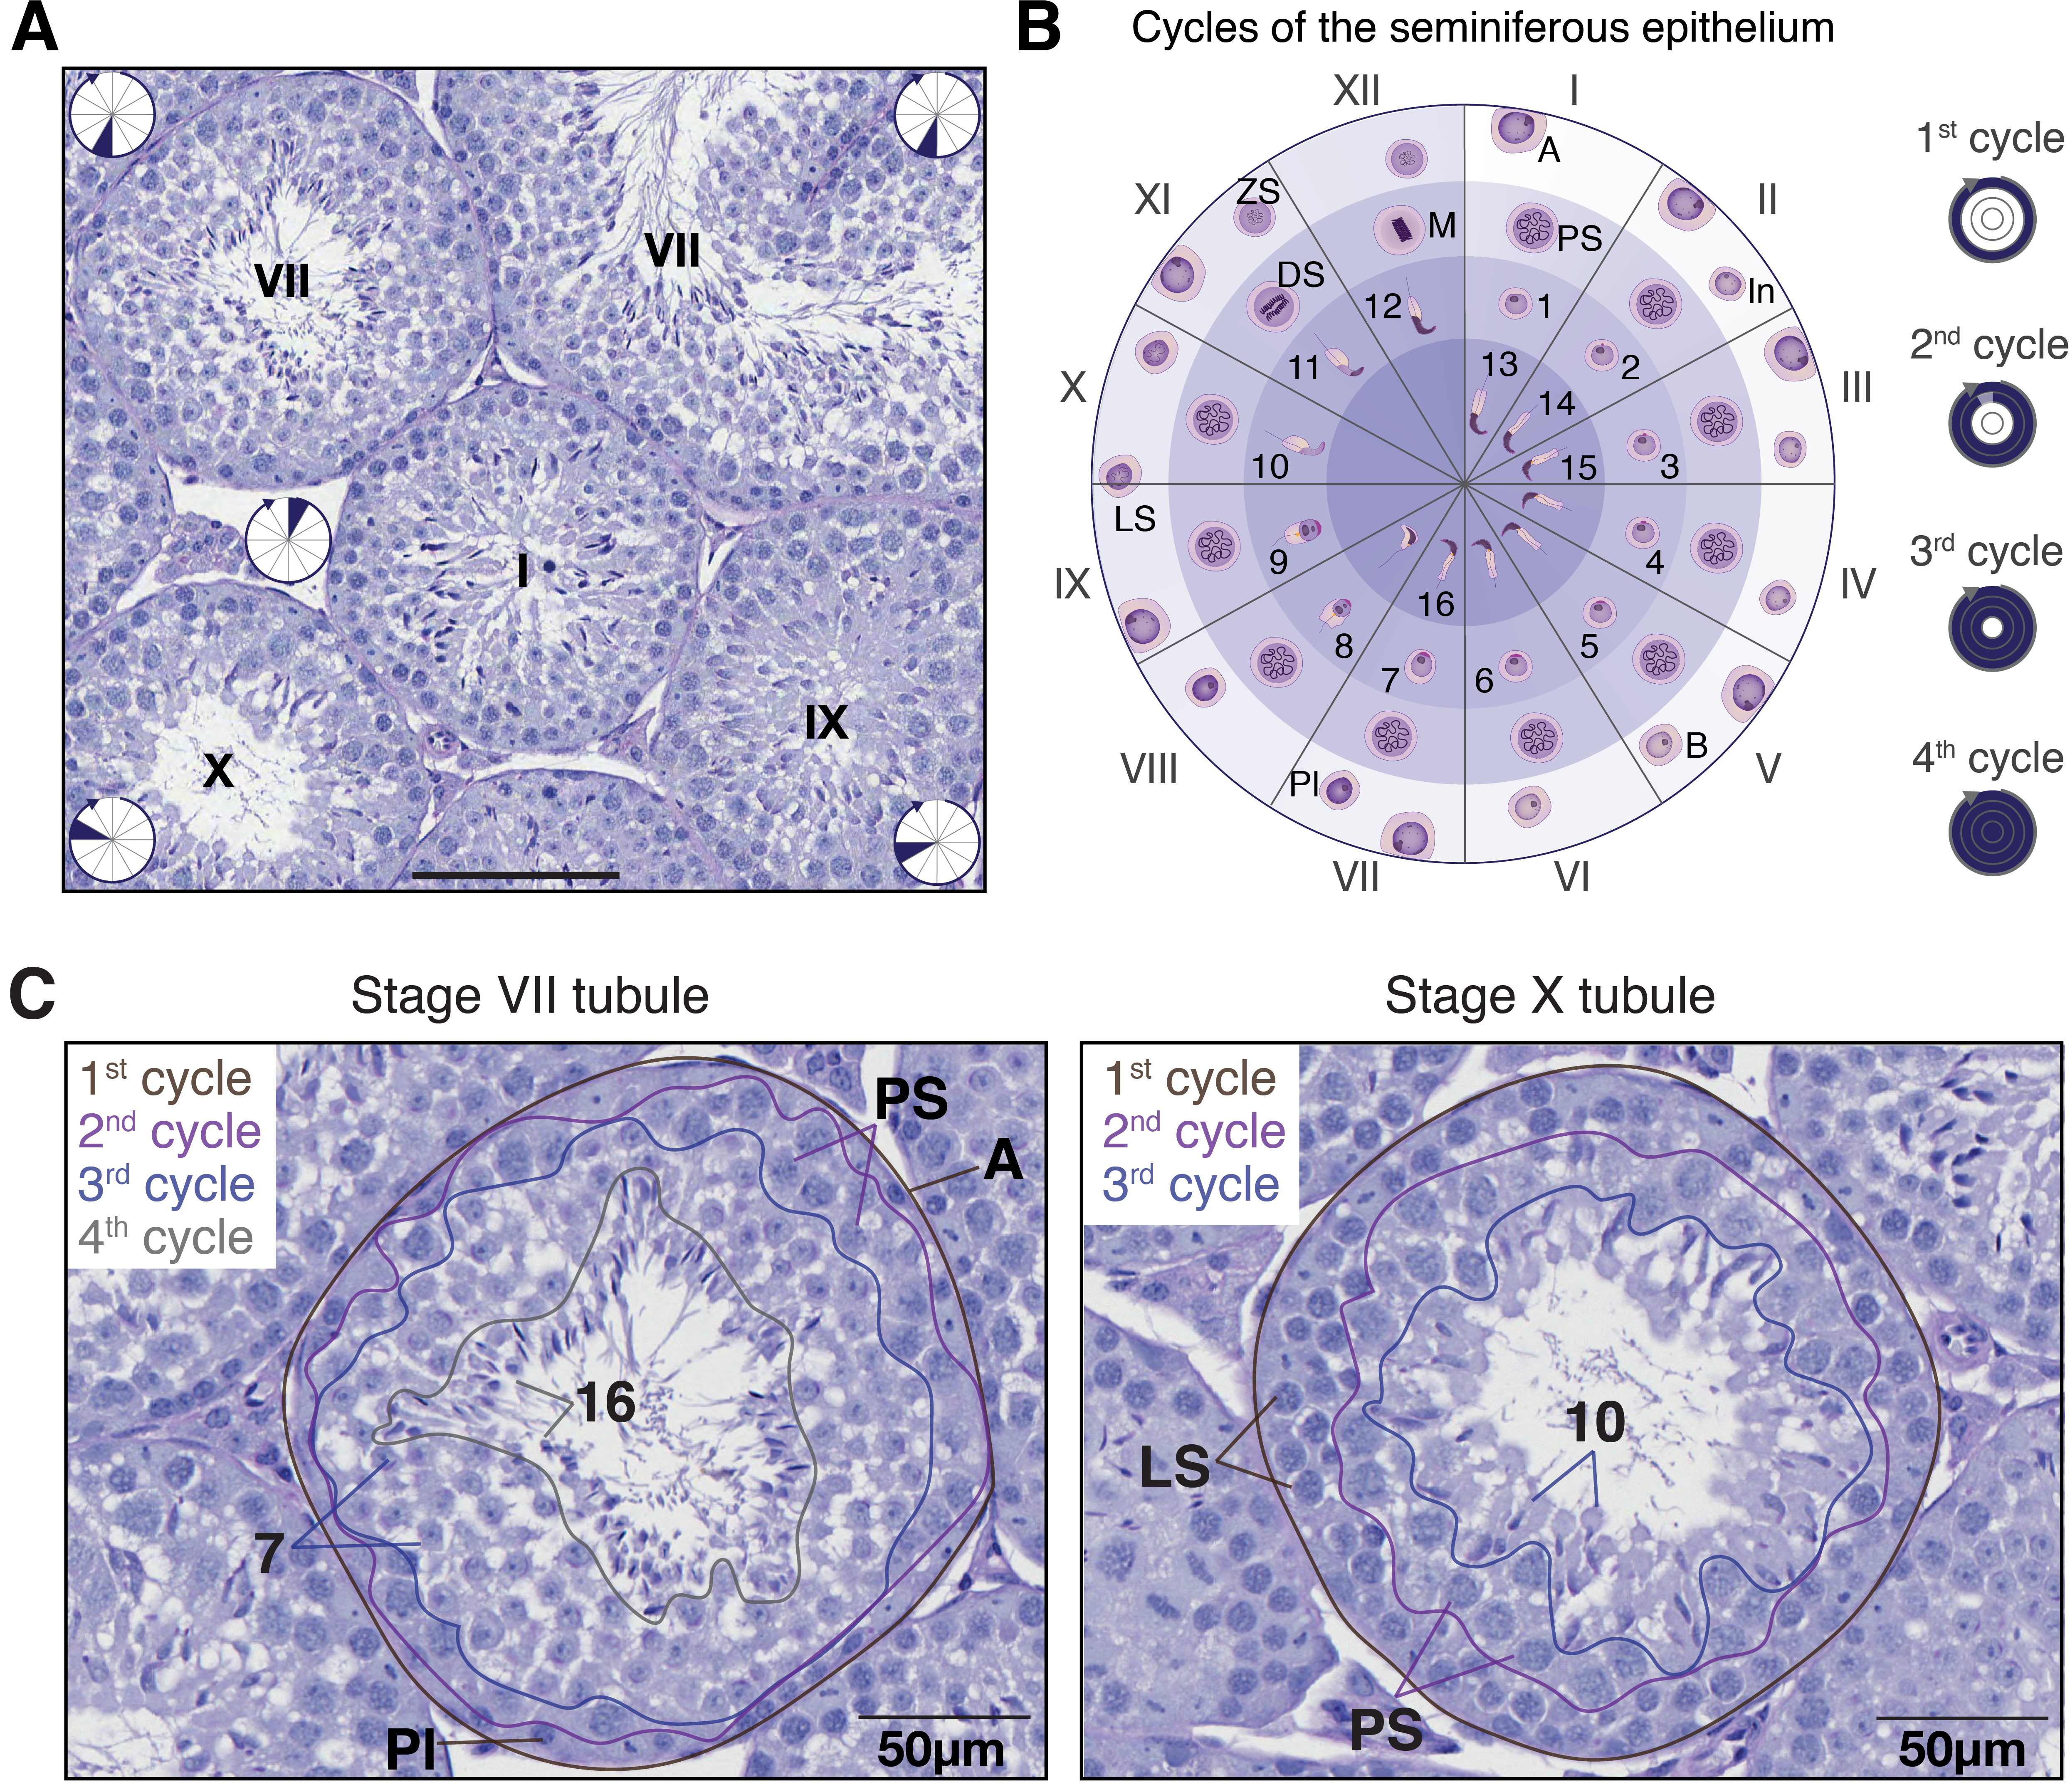
\includegraphics[width=\textwidth]{Fig_1.png}
\caption[Staging of the testicular seminiferous epithelium]{\textbf{Staging of the testicular seminiferous epithelium (full legend on next page).}\\
\textbf{(A)} Periodic Acid Schiff (PAS)-stained testis cross-section showing a number of seminiferous tubules at different epithelial stages (displayed as Roman numerals). Within each tubule, the inset circle refers to the corresponding section in (B). Scale bar represents 100 µm, \textbf{(B)} Schematic representation of the 12 stages of the seminiferous epithelium in mice. The colour gradient within the circle indicates the differentiation path of germ cells with the layers corresponding to individual cycles of the epithelium. The circle is divided into 12 section, each corresponding to one epithelial stage displaying the characteristic germ cells. Within each section, cells are positioned across the different layers according to their emergence during consecutive cycles, each being 8.6 days apart with more mature cells moving towards the centre, \textbf{(C)} Higher magnification of two tubules depicted in (A). The PAS-stained cross-sections show tubules in Stage VII and Stage X, with the different cell layers indicated by coloured lines. Stage VII tubules contain 4 different layers with germ cells from different generations that are approximately 8.6 days apart, whereas Stage X tubules only contain three layers. Cell types are labelled as: A – type A spermatogonia (SG), In – intermediate SG, B – type B SG, Pl – preleptotene spermatocytes (SCs), L – leptotene SCs, Z – zygotene SCs, P – pachytene SCs, D – diplotene SCs, M – metaphase I and II, 1-8 round spermatids (1-8), 9-16 elongating spermatids (9-16).}
\label{fig3:cell_staging}
\end{figure}

\newpage

To fully elucidate the molecular genetics of germ cell development, it is crucial to sample the full spectrum of germ cells present in testes of adult animals. For this purpose, we employed an unbiased droplet-based single-cell RNA-Sequencing (scRNA-Seq) approach. The 10X Genomics\texttrademark{} platform was used to generate hundreds of thousands of Gel beads in EMulsions (GEM). Around 80\% of generated oil droplets capture barcoded gel beads in 8 channels in parallel. Each barcode consists of a sequencing adapter and primer, a 14bp barcode from a pool of 750,000 barcodes, a 10bp UMI and a 30bp poly-dT oligotide to capture poly-A mRNA \citep{Zheng2017}. GEMs are fused with individual cells at a low concentration and cell lysis begins instantaneous. mRNA molecules are capture by the poly-dT barcode and enzymes needed for reverse transcription are released from the gel beads. Each cDNA therefore contains a transcript specific UMI and a GEM specific barcode making demultiplexing possible. Barcoded cDNA is pooled for PCR amplification and library preparation \citep{Zheng2017}. \\

We used the transcriptomic profiles of thousands of single germ cells to characterize the complex transcriptional dynamics of spermatogenesis at high-resolution. To confidently identify and label cell populations throughout the developmental trajectory, we profiled cells from juvenile testes during the first wave of spermatogenesis. In juveniles, spermatogenesis has only progressed to a defined developmental stage, and therefore allowed us to unambiguously identify the most mature cell type by comparison with adult. The correct labelling of cell types was then used to dissect differentiation processes such as meiosis and spermiogenesis. Furthermore, juvenile samples enriched for spermatogonia which allowed us to characterize spermatogonial differentiation. Another major developmental process during spermatogenesis is the inactivation and reactivation of the X chromosome, which is subject to transcriptional silencing as a consequence of asynapsis \citep{Turner2007}. By combining bulk and single-cell RNA-Seq approaches with chromatin profiling, we identified that \textit{de novo} activated X-linked genes carry distinct chromatin signatures with high levels of repressive H3K9me3 in spermatocytes. \\

Finally, after fully characterising the transcriptional changes during spermatogenesis, I used the regression model presented in the previous chapter to study changes in transcriptional variability over the differentiation time-course. To this end, I generated \emph{post hoc} posterior distribution of linear regression coefficients to statistically test whether individual genes increase or decrease in variability. Furthermore, the clustering of variability profiles showed that rapid transcriptional changes during differentiation can cause peaks in such variability profiles.

\newpage
%!TEX root = ../chapter3.tex
%******************************
%	 Results 
%*****************************

\section{Droplet based single-cell RNA sequencing of mouse testis}
\subsection*{High-resolution profiling by single-cell RNA-seq captures the unidirectional differentiation of germ cells during adult spermatogenesis}

Spermatogenesis is a recurrent differentiation process that produces male gametes within testicular seminiferous tubules \textbf{(Fig.~\ref{fig3:cell_staging}A)}. The seminiferous epithelium in the mouse is classified into twelve distinct stages, based on the combination of cell types present \textbf{(Fig.~\ref{fig3:cell_staging}B)}. Tubules cycle asynchronously and continuously through these stages and adult testis contain tubules in every possible epithelial stage \textbf{(Fig.~\ref{fig3:cell_staging}}. \\

\begin{figure}[!h]
\centering
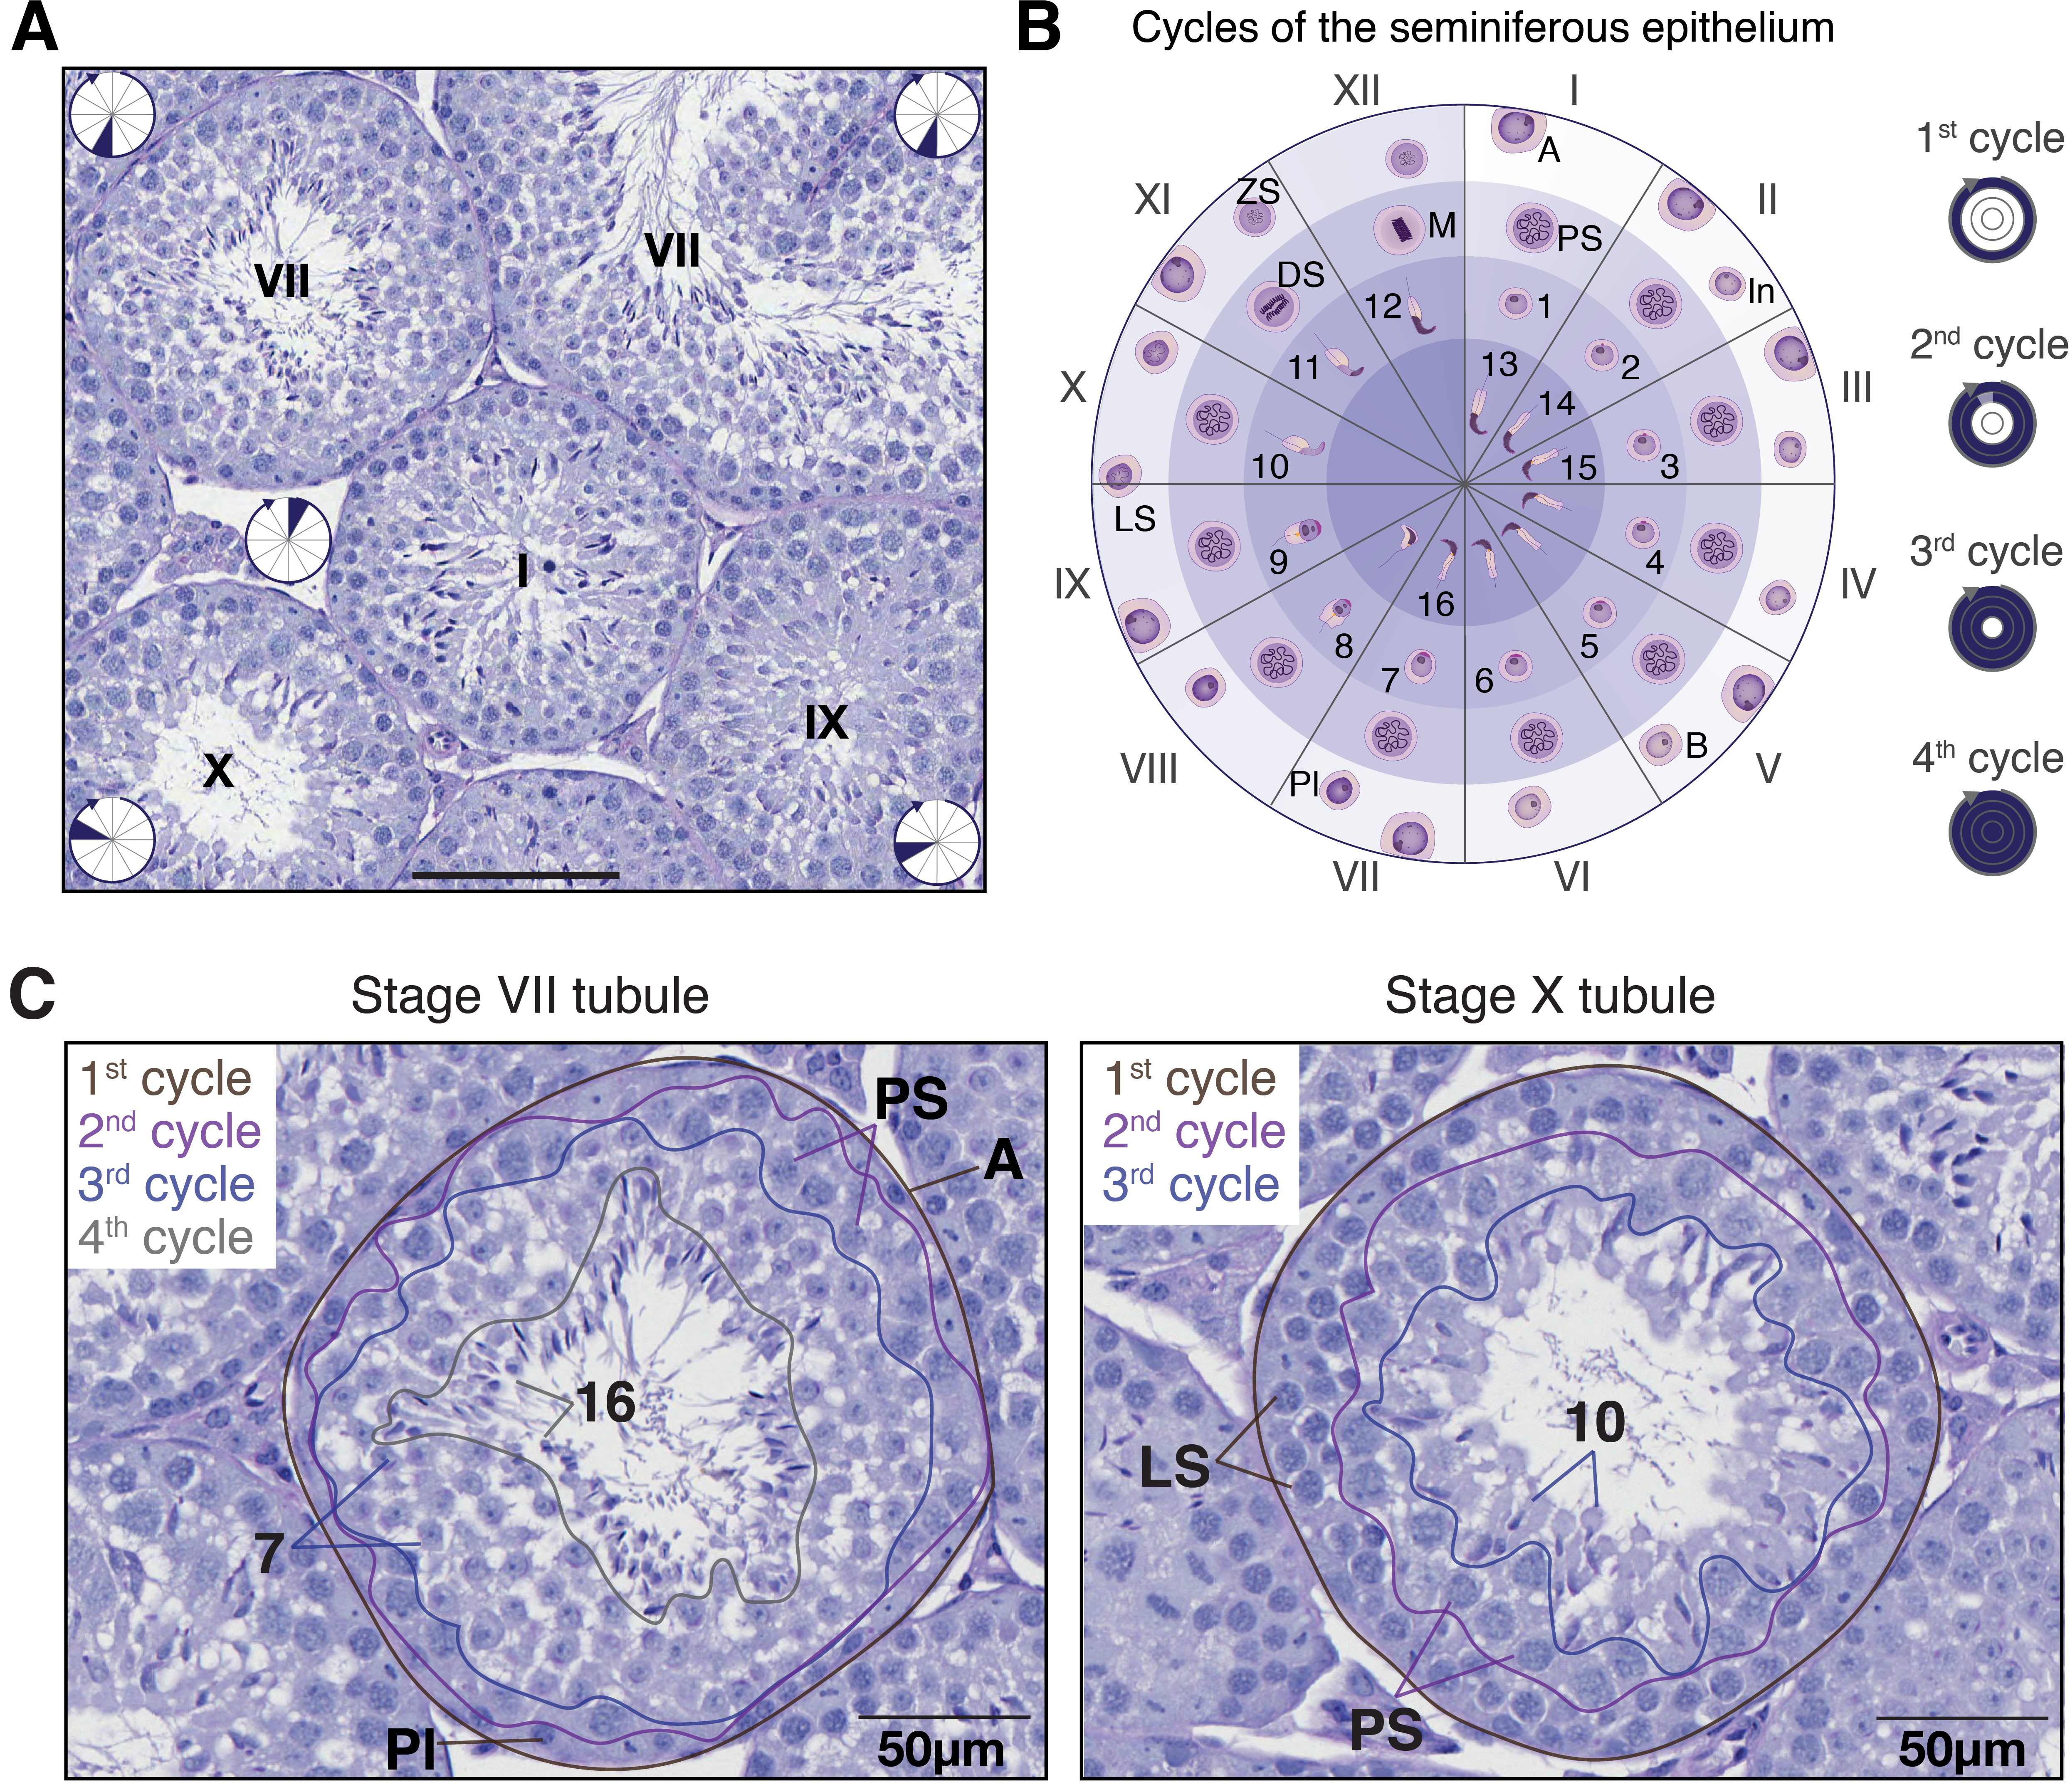
\includegraphics[width=\textwidth]{Fig_1.png}
\caption[Staging of the testicular seminiferous epithelium]{\textbf{Staging of the testicular seminiferous epithelium (full legend on next page).}\\}
\label{fig3:cell_staging}
\end{figure}

\newpage

\captionsetup[figure]{list=no}
\addtocounter{figure}{-1}   
\captionof{figure}{\textbf{Staging of the testicular seminiferous epithelium (continued).}\\
\textbf{(A)} Periodic Acid Schiff (PAS)-stained testis cross-section showing a number of seminiferous tubules at different epithelial stages (displayed as Roman numerals). Within each tubule, the inset circle refers to the corresponding section in (B). Scale bar represents 100 µm; original magnification 200X. \textbf{(B)} Schematic representation of the 12 stages of the seminiferous epithelium in mice. The colour gradient within the circle indicates the differentiation path of germ cells with the layers corresponding to individual cycles of the epithelium. The circle is divided into 12 section, each corresponding to one epithelial stage displaying the characteristic germ cells. Within each section, cells are positioned across the different layers according to their emergence during consecutive cycles, each being 8.6 days apart with more mature cells moving towards the centre.  Cell types are labelled as: A – type A spermatogonia (SG), In – intermediate SG, B – type B SG, Pl – preleptotene spermatocytes (SCs), L – leptotene SCs, Z – zygotene SCs, P – pachytene SCs, D – diplotene SCs, M – metaphase I and II, 1-8 round spermatids, 9-16 elongating spermatids. \textbf{(C)} Higher magnification of two tubules depicted in (A). The PAS-stained cross-sections depict tubules in Stage VII and Stage X, with the different cell layers indicated by coloured lines. Stage VII tubules contain 4 different layers with germ cells from different generations that are approximately 8.6 days apart, whereas Stage X tubules only contain three layers. Each layer contains a certain set of germ cells depending on the epithelial stage. Stage VII contains preleptotene spermatocytes (Pl) in the first layer, pachytene spermatocytes (P) in the second layer, S7 round spermatids (7) in the third layer and S16 elongating spermatids in the fourth innermost layer. Stage X tubules contain leptotene spermatocytes (L) in the first layer, pachytene spermatocytes (P) in the the second layer and only one generation of round-to-elongating spermatids at S10 (10) in the innermost layer. Original magnification 400X.  \\}
\captionsetup[figure]{list=yes}

To fully dissect mouse spermatogenesis, we primarily analysed droplet based single-cell RNA sequencing using the 10X Chromium technology \citep{Zheng2017}. For this, mouse testes were enzymatically dissociated and single-cell suspensions at a concentration of ~300,000 cells/ml was loaded into one channel of the ChromiumTM Single Cell A Chip (10X Genomics), aiming for a recovery of 4000-5000 high-quality cells. Cells were isolated from specifically staged juvenile (between postnatal days 6 and 35) and adult (8-9 weeks) C57BL/6J (B6) mice \textbf{(Table \ref{tab3:QC_scRNAseq})}. To obtain gene-specific transcript counts for droplet based scRNA-Seq, the Cell Ranger \emph{count} function with default settings was used to align and count unique molecular identifiers (UMIs) per sample. This software retains cells with similar UMI distributions \citep{Zheng2017} which we label as "high-quality" transcriptomes. We use this default threshold to obtain high-quality cells with large numbers of UMIs. After merging all samples, we filtered out cells that express less than 1000 genes. Furthermore, we exclude cells with more than 10\% of reads mapping to the mitochondrial genome. \\
Using the Cell Ranger default threshold leads to the exclusion of cells with lower transcriptional complexity. We therefore used the emptyDrops function provided in the \emph{DropletUtils} Bioconductor package \citep{Lun2018} to statistically distinguish empty droplets from genuine cells (controlling the FDR to 1\%). After merging true cells across all samples, we filtered out cells with less than 500 genes expressed. Furthermore, we excluded cells with more than 10\% or mitochondrial genes expressed \textbf{(Table \ref{tab3:QC_scRNAseq})}. The transcriptomes of quality filtered cells were normalized using the scran package \citep{Lun2016pooling}. After quality control and filtering, we retained more than 20,000 high-quality single cells and over 46,000 cells including the once with lower transcriptional complexity \textbf{(Table \ref{tab3:QC_scRNAseq})}. \\
This two-way approach allows us to (i) dissect molecular processes using high-quality cells and capture all testicular cell types, even cells with low transcriptional complexity.\\

Additionally, for juvenile samples, we generated whole-tissue bulk RNA sequencing, as well as mapping chromatin state in purified cell populations using CUT\&{}RUN (Cleavage Under Targets \& Release Using Nuclease) \citep{Skene2018}. With this, we additionally generated 30 bulk RNA-Seq libraries and 8 CUT\&{}RUN libraries.The full experimental set-up can be seen in \textbf{Fig.~\ref{fig3:experimental_design}}.

\begin{figure}[!h]
\centering
\includegraphics[width=\textwidth]{Fig_2.png}
\caption[Experimental design to dissect mouse spermatogenesis]{\textbf{Experimental design to dissect mouse spermatogenesis.}\\
Overview of the experimental design yielding bulk RNA-Seq, droplet-based scRNA-Seq and chromatin profiling on FACS-purified cells using CUT\&{}RUN from one testis while using the contralateral testis for matched histology.}
\label{fig3:experimental_design}
\end{figure}

To remove batch-specific effects that arise when samples are prepared and sequenced in different experiments \textbf{(Tables \ref{tab3:QC_scRNAseq})}, we used the \emph{mnnCorrect} function implemented in the \emph{scran} package \citep{Haghverdi2018}. We used the top 1000 genes with highest biological variation across all samples as informative genes for batch correction. The \emph{mnnCorrect} function takes transcriptional profiles of cells isolated from adult B6 mice as first input and uses this dataset as reference for cell mapping. This approach maps the juvenile samples onto the adult B6 \textbf{(Fig.~\ref{fig3:cell_types}A)}

\begin{table}[ht	]
\centering
\caption[Quality filtering of scRNAseq data]{\textbf{Quality filtering of scRNAseq data.} \\
Quality metrics of droplet-based scRNA-Seq. Sample: Stage and genotype information for all samples. Library: sample identifier. CellRanger filter: Number of retained cells after default thresholding using the CellRanger counts function.  After quality control: Number of cells obtained after quality control. Assigned Cell Type: Number of cells that fall into annotated clusters (removing outlying cells). EmptyDrops filter: Number of cells retained after using the emptyDrops function controling the FDR to 1\%. EmptyDrops quality control: Number of cells obtained after quality control of the \emph{emptyDrops} filtered cells.}
\label{tab3:QC_scRNAseq}
\begin{tabular}{lllllll}
\toprule
\textbf{Sample} & \textbf{Library} & \textbf{CellRanger} & \textbf{After} & \textbf{Assigned} & \textbf{EmptyDrops} & \textbf{EmptyDrops} \\
& & \textbf{filter} & \textbf{QC} & \textbf{Cell Type} & \textbf{filter} & \textbf{QC} \\
\midrule
B6     & do17815 & 1157              & 1157                  & 1123               & 4467              & 3400                       \\
\midrule
B6     & do17816 & 2198              & 2198                  & 2092               & 6145              & 4603                       \\
\midrule
P10    & do17821 & 3229              & 3213                  & 3212               & 4976              & 4202                       \\
\midrule
P15    & do18195 & 4258              & 4258                  & 4014               & 14050             & 13168                      \\
\midrule
P20    & do17824 & 1775              & 1775                  & 1662               & 9400              & 7491                       \\
\midrule
P25    & do18196 & 4334              & 4334                  & 4130               & 8038              & 6802                       \\
\midrule
P30    & do17825 & 2278              & 2278                  & 2211               & 5393              & 4958                       \\
\midrule
P35    & do17827 & 3160              & 3160                  & 3004               & 49002             & 10683                      \\                 
\bottomrule   
\end{tabular}
\end{table}

To identify cell types across all samples, batch corrected transcriptomes were clustered using a graph-based approach. A shared nearest-neighbour (SNN) graph \citep{Xu2015} was constructed considering 3 shared nearest neighbours using the \emph{buildSNNGraph} function in scran. In the next step, a multi-level modularity optimization algorithm was used to find community structure in the graph \citep{Blondel2008} implemented in \emph{igraph} R package. Cells in small clusters that show unclear identities were excluded from down-stream analysis.\\
We next aimed to annotate clusters based on the expression of marker genes. The adult B6 samples were used to identify marker genes for all germ cell-types present in testes. To this end, we performed differential expression testing across multiple pairwise comparisons. To detect cluster-specific marker genes, the \emph{findMarkers} function implemented in \emph{scran} was used on the log$_2$-transformed normalized counts while providing the cluster labels \textbf{(Fig.~\ref{fig3:cell_types}B)}. \\

On a broad level and by visualizing the expression of detected marker genes, we identified the following cell types: spermatogonia (based on \textit{Dmrt1} expression, \citep{Matson2010}), spermatocytes (\textit{Piwil1}, \citep{Deng2002}), round and elongating spermatids (\textit{Tex21} and \textit{Tnp1}, respectively, \citep{Fujii2002}), as well as the main somatic cell types of the testis, Sertoli (\textit{Cldn11}, \citep{Mazaud-Guittot2010}) and Leydig cells (\textit{Fabp3}, \citep{Oresti2013}) \textbf{(Fig.~\ref{fig3:cell_types}B)}. Using a dimensionality reduction technique for visualization (t-distributed Stochastic Neighbour Embedding; \textbf{Fig.~\ref{fig3:cell_types}C}), the germ cell types from spermatocytes to elongating spermatids formed a continuum, which recapitulated the known developmental trajectory.

\begin{figure}[!h]
\centering
\includegraphics[width=0.8\textwidth]{Fig_3.png}
\caption[Droplet based scRNAseq of mouse spermatogenesis]{\textbf{Single-cell RNA-Seq captures a continuum of germ cell types during adult spermatogenesis.}\\
\textbf{(A)} tSNE representation of juvenile cells that were mapped to cells isolated from adult mice. Grey dots indicate all cells from adult animals that were used as a reference for cell mapping (see Methods). Coloured dots represent cells isolated at each sampled stage during the first wave of spermatogenesis. Clustering has been perfomed across all cells after cell mapping (see Methods). SG: Spermatogonia, M: Meiosis, IL: Imature Leydig, PTM: Peritubular Myoid Cells, EC: Endothelial Cells, tMg: testicular Marcophages. \textbf{(B)} tSNE representation of scRNA-Seq data from adult B6 mice with the colour gradient representing the expression of known marker genes for two somatic cell types and the main germ cell types. The x- and y-axis represent the first and second dimension of tSNE respectively. The colour legend shows log2-transformed, normalized expression counts. \textbf{(E)} Graph-based clustering (see Methods) identifies different sub-stages within major germ cell populations. 
}
\label{fig3:cell_types}
\end{figure}

\section{Developmental staging of mouse spermatogenesis}
\subsection*{Staged developmental mapping of the first wave of spermatogenesis defines germ cell identity}

Historically, sub-staging of the major cell types within the testis was based on changes in nuclear or cellular morphology \citep{Oakberg1956,  Oakberg1956a}. Previous attempts to complement morphology with molecular signatures have been limited to FACS-based and sedimentation assays, where the resolution was unable to differentiate between sub-cell-types \citep{Bastos2005, Gaysinskaya2014, Lam1970, Meistrich1977, Romrell1976, Soumillon2013}. While a mixture of all spermatogenic cell types co-exists in the adult, the first wave of spermatogenesis during juvenile development is more synchronised. Starting around mouse postnatal day P4, spermatogonia begin to differentiate, forming the first generation of spermatocytes as early as P10, round spermatids by P20, and completing the first wave of spermatogenesis with the production of mature spermatozoa between P30 and P35 \textbf{(Fig.~\ref{fig3:1st_wave}A)} \citep{Bellve1977, Janca1986, Nebel1961}.\\
 
We exploited this first spermatogenic wave to generate thousands of high-resolution single-cell transcriptional profiles of morphologically well-defined cell populations. For this, we sampled multiple time points during the first wave to identify the most mature (differentiated) cell types. Based on known sperm developmental transitions, we chose six time points between P10 and P35 from which to generate single-cell RNA-Seq libraries \textbf{(Fig.~\ref{fig3:1st_wave}A)}. For each juvenile experiment, we found that the population of developing germ cells was strongly enriched at the expected developmental stage, as quantified by the percentage of cells in each cell-type cluster \textbf{(Fig.~\ref{fig3:1st_wave}B and C)}. By associating these cell types with the corresponding cell types in the adult trajectory, we unambiguously assigned molecular and histological signatures to cells during adult spermatogenesis.\\

For instance, at P15 the majority of cells are spermatogonia and spermatocytes progressing through the mid-pachytene stage, in accord with the appearance of the sex body \citep{Turner2004}. Interestingly, less mature cell types are also present at this time point (and later time points), supporting recent reports that the first wave of spermatogenesis is less synchronized than previously anticipated \citep{Snyder2010}. At P20, we detect an enrichment for spermatocytes, cells undergoing meiotic cell division, and a small group of early round spermatids. This population structure is in line with matched histology, which shows a large number of tubules in late stages IX-XII and the first occurrence of early round spermatids \citep{Bellve1977}.\\
Spermatids first reach the elongating state between P24 and P26 \citep{Janca1986}. At P25, we observed cells matched to our first ten clusters of spermatids, which we then labelled according to morphologically-defined spermatid substages S1 – S10 \textbf{(Fig.~\ref{fig3:1st_wave}C)}. At P30 and P35, we observed a relatively even distribution of cells across all groups, closely resembling the adult distribution up to S14, indicating that the first wave of spermatogenesis is complete. 

\begin{figure}[!h]
\centering
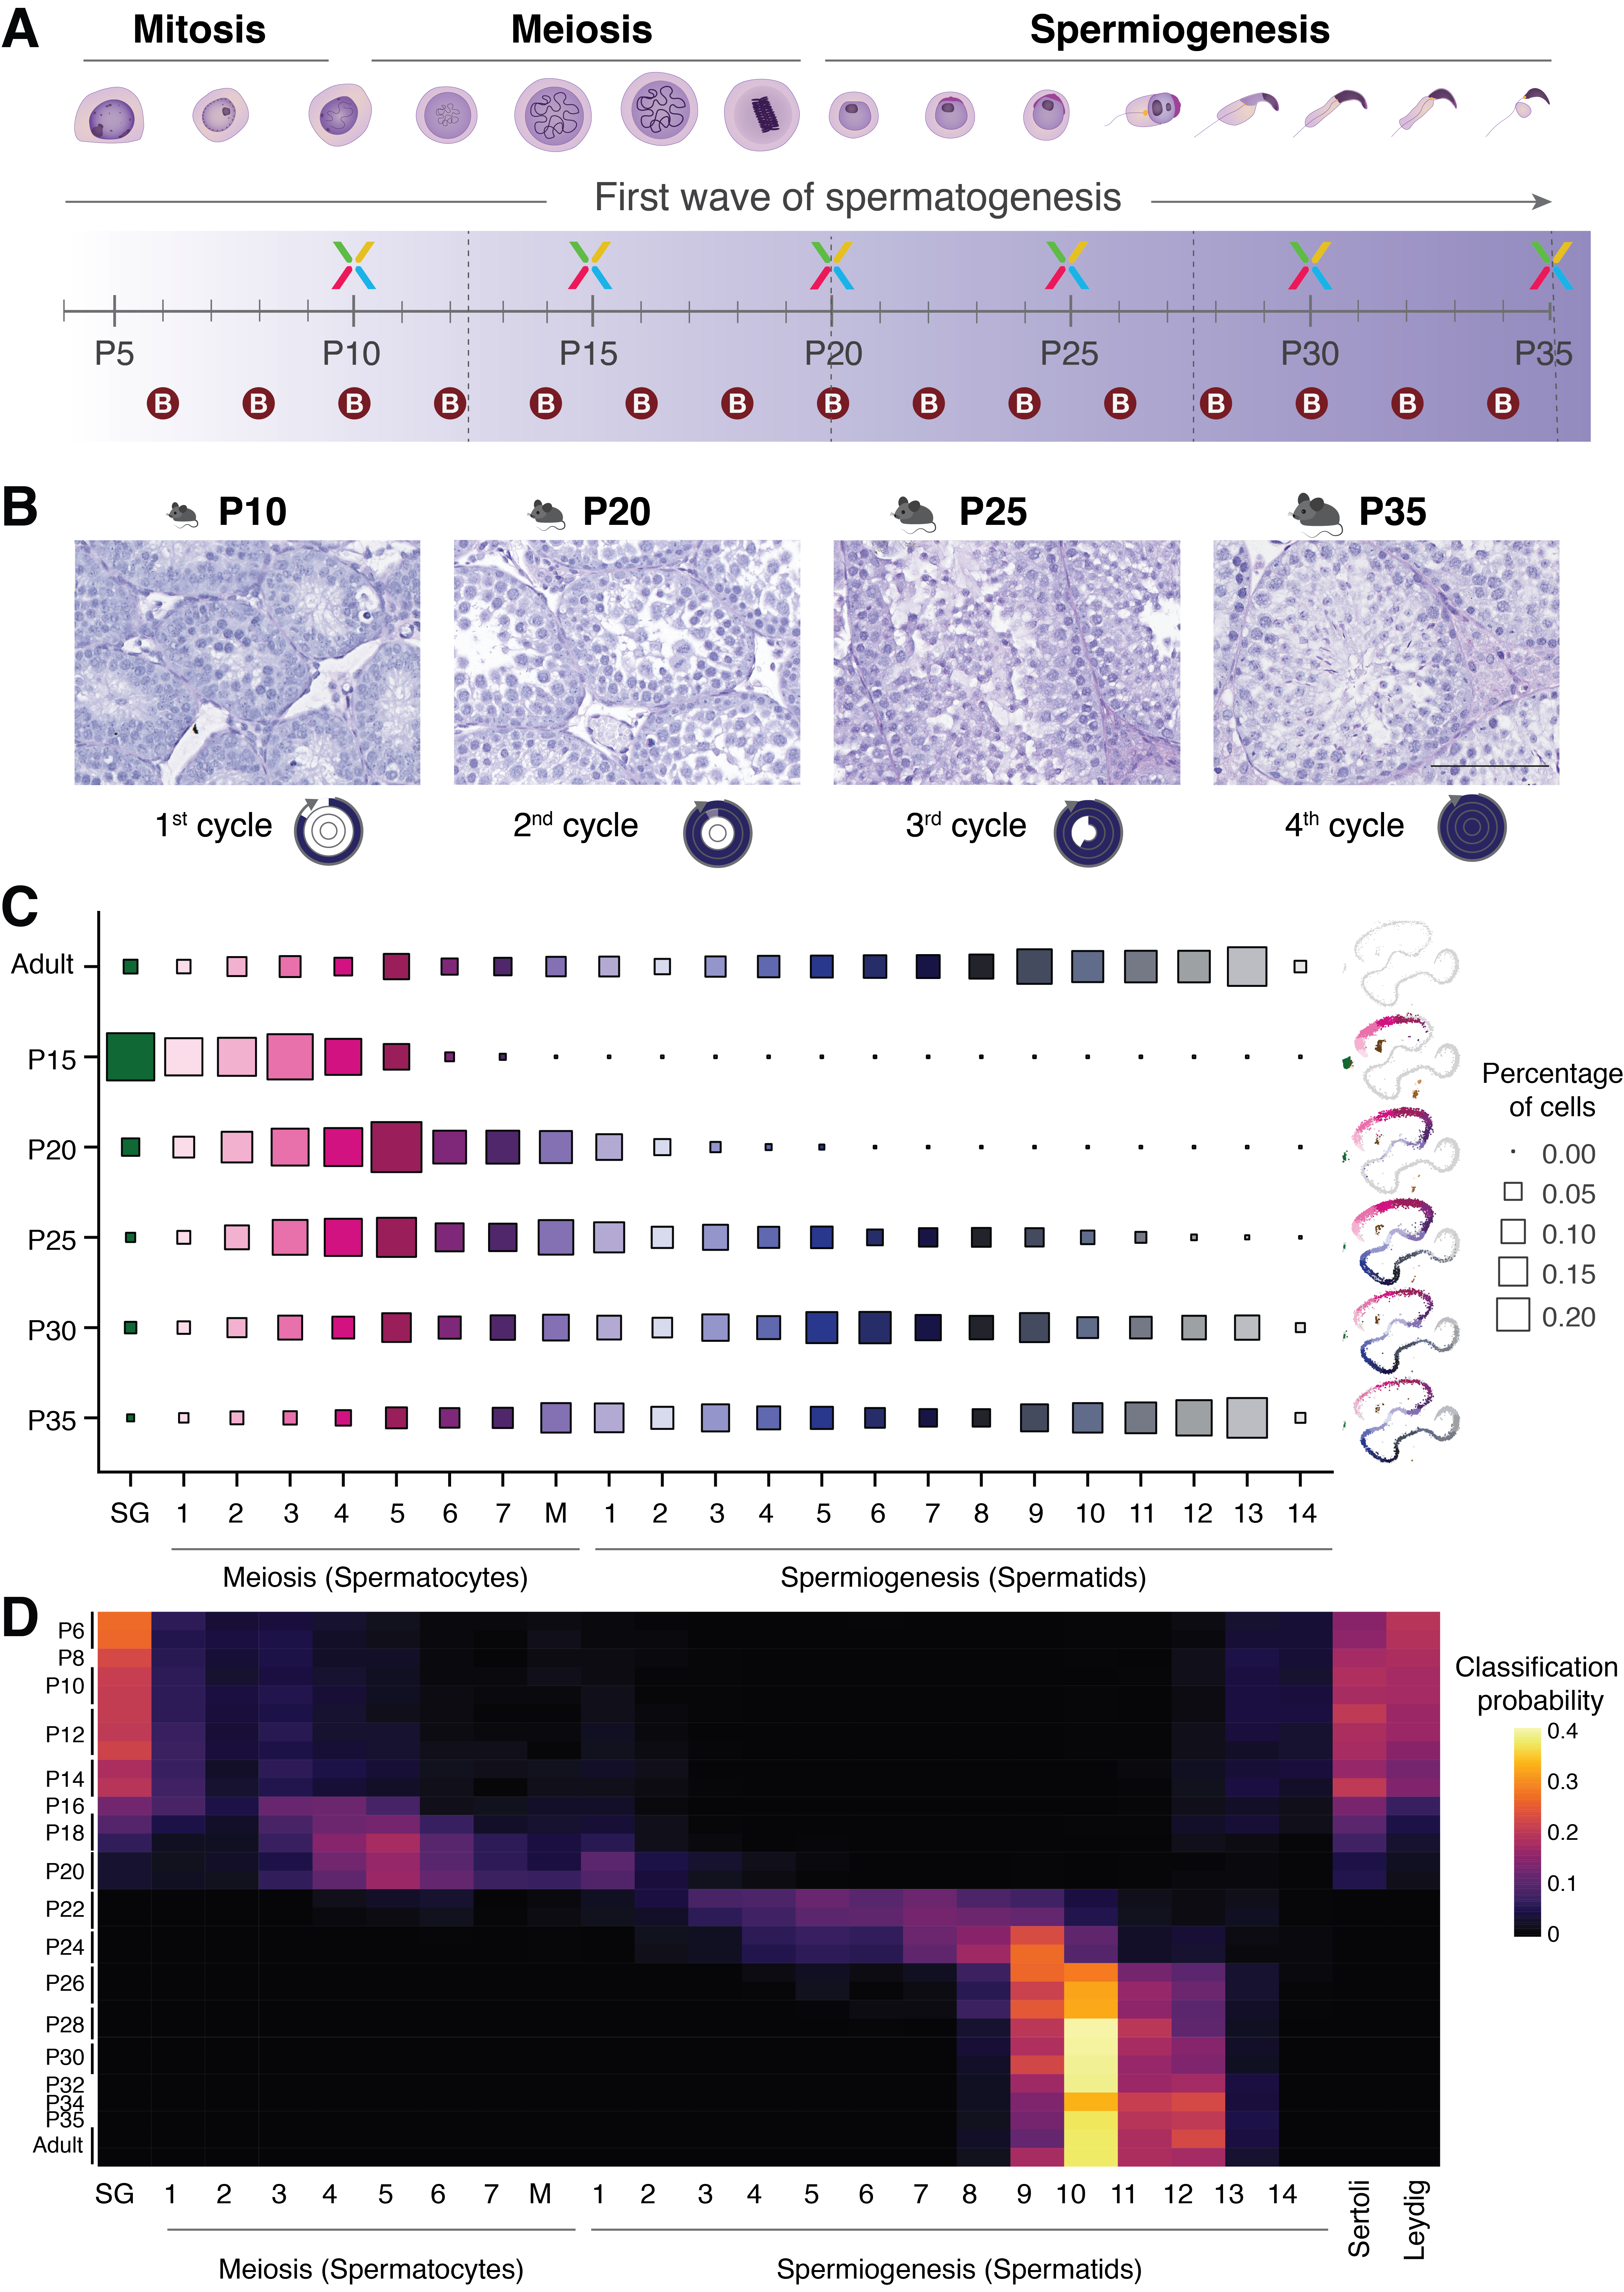
\includegraphics[width=0.85\textwidth]{Fig_4.png}
\caption[Staging of cell types during mouse spermatogenesis]{\textbf{Cell type classification by developmental mapping of time points during the first wave of spermatogenesis (full legend on next page).}}
\label{fig3:1st_wave}
\end{figure}

\newpage

\captionsetup[figure]{list=no}
\addtocounter{figure}{-1}   
\captionof{figure}{\textbf{Cell type classification by developmental mapping of time points during the first wave of spermatogenesis (continued).}\\
\textbf{(A)} Schematic representation of the major germ cell types and their corresponding developmental processes. Spermatogonia differentiate undergoing mitotic cell divisions before forming spermatocytes that divide by meiotic division. Spermatids differentiate throughout spermiogenesis to form mature sperm. The timeline in the lower panel indicates at which point during the first wave of spermatogenesis samples were harvested for the generation of scRNA-Seq (X) or bulk RNA-Seq (B) data. \textbf{(B)} Representative images of seminiferous tubules from PAS-stained tissue cross-sections from animals harvested at different postnatal (P) time points during the first wave of spermatogenesis. The approximate timing of the stage and cycle of the tubule is illustrated below in the form of a circle (see Fig.~\ref{fig3:cell_staging}B). \textbf{(C)} The percentage of cells allocated to each cell cluster for each juvenile and adult sample is represented by the size of squares with the colours corresponding to the clusters depicted in Fig. \ref{fig3:cell_types}C. tSNEs on the right-hand side of each panel (juvenile samples only) illustrate progress through spermatogenesis.  SG – spermatogonia, M – metaphase. \textbf{(D)} Probabilistic mapping of bulk RNA-Seq libraries to the cell clusters identified in the adult scRNA-Seq data using a random forest approach. The colour gradient indicates the probability with which a bulk sample can be assigned to the specific cell cluster.  \\}
\captionsetup[figure]{list=yes}

To further validate the identity of the cell clusters, we used bulk RNA-Seq from testis collected during the first wave of spermatogenesis every two days between P6 and P34 \textbf{(Fig.~\ref{fig3:1st_wave}A)}. We used a regression approach to link the bulk samples to the transcriptomic profiles of single cells. Using the top 50 cluster-specific marker genes for spermatogonia, all spermatocyte groups, all spermatid groups, sertoli and leydig cells, we trained a random forest classifier (implemented in the \emph{randomForest} R package \citep{Liaw2002}) on 2000 cells isolated from adult B6 testes. Model testing was performed on the remaining 1215 cells isolated from adult B6 testes. Prior to training and testing, log$_2$-transformed, normalized counts were scaled by computing the Z score for each gene. Probabilistic prediction was performed using the Z score of log$_2$-transformed, normalized bulk RNA-Seq reads of the input genes. This confirmed that between P6 – P14 spermatogonia and somatic cells show the highest contribution to the transcriptomic profile \textbf{(Fig.~\ref{fig3:1st_wave}D)}. Between P16 and P20 we observed the emergence of spermatocyte-specific gene expression signatures, after which spermatids become the transcriptionally dominant cell type. By P26, spermatids reach the elongating state where transcription is uniformly shut-down due to the beginning of the histone-to-protamine transition \citep{Steger1999}; following this, changes in RNA content are mostly due to degradation. Bulk transcriptional profiles can therefore only be classified up to S10, because transcription is largely inactive thereafter.\\

In sum, by combining transcriptional and histological analyses at specific stages during the first wave of spermatogenesis, we assigned transcriptional profiles to specific, morphologically defined germ cell types.

\section{Under-represented cell types in spermatogenesis}
\subsection*{Identification of under-represented and transcriptionally silent cell types in adolescent testes}

In addition to assigning the dominant cell types in germ cell development, we further exploited the juvenile samples to analyse the highly enriched cell types that are rare in adult testes, including somatic support cells, spermatogonia and the earliest spermatocytes.  Through the first wave of spermatogenesis, the ratio between germ cells and somatic cells increases; therefore, to study heterogeneity within the somatic cell population, we focused on the P10 stage, where somatic cells are relatively more frequent. As expected, we readily identified substantial numbers of Sertoli and Leydig cells, which are the main somatic cell types in adult \citep{Griswold1998, Haider2004}.  In addition, we newly identified a large population of immature Leydig cells, based on \textit{Dlk1} expression \citep{Lottrup2014}. Furthermore, we detected the cells that form the basal lamina such as peritubular myoid cells (PTM, \textit{Acta2}, \citep{Cool2008}), vascular endothelial cells (\textit{Tm4sf1}, \citep{Shih2009}), and testicular macrophages (\textit{Cd14}, \citep{Kitchens2000}) \textbf{(Fig.~\ref{fig3:somatic_cells}A and B)}. By performing differential expression analysis, we identified novel markers for these cell populations that are relatively under-represented in adult testes.\\

\begin{figure}[!h]
\centering
\includegraphics[width=\textwidth]{Fig_5.png}
\caption[Enrichment of under-represented somatic cell types in juvenile samples]{\textbf{Enrichment of underrepresented somatic cell types in juvenile samples.} \\
\textbf{(A)} tSNE representation of cells isolated from P10 animals that were mapped to cells from adult mice. Cell types were identified by unbiased, graph-based clustering and annotated after marker gene extraction. SG: Spermatogonia, SC: Spermatocytes, IL: Immature Leydig, PTM: Peritubular Myoid Cells, EC: Endothelial Cells, tMg: testicular Macrophages. \textbf{(B)} Heatmap representation of cell type-specifc marker genes. Bolded genes indicate previously described markers for the following cell types: Sertoli cells (\textit{Cst12}), early spermatocytes (\textit{Sycp1}), spermatogonia (\textit{Dmrt1}), immature leydig cells (\textit{Dlk1}), endothelial cells (\textit{Acta2}), peritubular myoid cells (\textit{Tm4sf1}), Leydig cells (Insl3), testicular macrophages (\textit{Cd14}). \textbf{(C)} PCA of spermatogonia (SG) and early spermatocytes (SC 1) from P10 and P15 animals. 
}
\label{fig3:somatic_cells}
\end{figure}

Identifying spermatogonial sub-populations in adult testes is greatly complicated by their rarity relative to other germ cell types \citep{Lukassen2018}. However, during early juvenile development spermatogonia are relatively enriched, which we exploited to further characterize their heterogeneity \textbf{(Fig. \ref{fig3:somatic_cells}A)}. By combining cells from P10 and P15, we obtained 1,186 transcriptional profiles that capture sub-populations during spermatogonial differentiation \textbf{(Fig. \ref{fig3:somatic_cells}B)}. To analyse transcriptomes of P10 and P15 samples, we performed batch correction between these samples as described above. We detected two clusters corresponding to undifferentiated spermatogonia (A$_\textnormal{undiff}$) based on their expression of \textit{Nanos3} and \textit{Zbtb16} \textbf{(Fig. \ref{fig3:somatic_cells}B and C)} \citep{Buaas2004, Lolicato2008}). These cells comprise A$_\textnormal{s}$, A$_\textnormal{paired}$, and A$_\textnormal{aligned}$ spermatogonia that decrease in stemness as they divide and gain competency to differentiate \citep{Suzuki2012}. Additionally, these cells express a number of marker genes also detected in undifferentiated human spermatogonial stem cells, such as \textit{Gfra1}, \textit{Bcl6} and \textit{Id4} \citep{Guo2017}. Based on the expression of \textit{Stra8} (Stimulated by retinoic acid 8), we can map the point at which spermatogonial differentiation is induced (A$_\textnormal{aligned}$-to-A$_\textnormal{1}$ transition), thus marking the beginning of differentiating spermatogonia (A$_\textnormal{diff}$) \citep{Endo2015}. A$_\textnormal{diff}$ are marked by the expression of \textit{Sohlh1} \citep{Ballow2006} and are highly proliferative, generating A$_\textnormal{1-4}$, Intermediate and B spermatogonia. Late differentiating spermatocytes express \textit{Dmrtb1} (also referred to as \textit{Dmrt6}), which mediates the mitosis-to-meiosis transition and quickly disappears in preleptotene spermatocytes. This latter population shows a second increase in Stra8 expression levels, which is necessary for initiation of meiosis \textbf{(Fig. \ref{fig3:somatic_cells}B and C)} \citep{Anderson2008, Endo2015, Zhang2014}. 

\newpage

\begin{figure}[!h]
\centering
\includegraphics[width=0.85\textwidth]{Fig_6.png}
\caption[Cellular heterogeneity during spermatogonial differentiation]{\textbf{Cellular heterogeneity during spermatogonial differentiation.} \\
\textbf{(A)} Schematic representation of spermatogonial differentiation including sub-stages of undifferentiated (A$_\textnormal{s}$, A$_\textnormal{paired}$, A$_\textnormal{aligned}$) and differentiating spermatogonia (A$_\textnormal{1}$, A$_\textnormal{2}$, A$_\textnormal{3}$, A$_\textnormal{4}$, In, B) (SGs) as well as Preleptotene (Pl). \textbf{(B)} Sub-structure detection in spermatogonia isolated from P10 and P15 animals. PCA was computed on transcriptomes after batch correction between P10 and P15 samples. The first three panels represent expression of known marker genes for undifferentiated (Undiff, \textit{Nanos3}) and differentiating (Diff, \textit{Stra8} and \textit{Dmrtb1}) spermatogonia. The colour scale shows log$_2$-transformed, normalized counts. The last panel overlays cluster identity by sub-clustering batch-corrected transcriptomes of spermatogonia. \textbf{(C)} Scaled, normalized expression counts of the top 15 marker genes per cell cluster. Column and row labels represent the cell clusters identified in the last panel of (B). The lower bar indicates the gradual differentiation from undifferentiated spermatogonia to preleptotene cells driven by two retinoic acid (RA) signals. }
\label{fig3:somatic_cells}
\end{figure}

The transition between differentiating spermatogonia and spermatocytes is a gradual process that occurs in stage VIII tubules when B spermatogonia divide and form preleptotene spermatocytes \citep{Anderson2008, Baltus2006}. We were therefore surprised not to observe a continuous differentiation trajectory bridging spermatogonia to spermatocytes textbf{(Fig. \ref{fig3:somatic_cells}C)}. One possible explanation is that leptotene and zygotene spermatocytes have decreased transcriptional activity \citep{Kierszenbaum1974, Monesi1965}, and are thus likely to be classified as empty droplets by the 10X CellRanger pipeline. 
To capture these transcriptionally quiescent cells, we applied a newly developed computational method that distinguishes between droplets capturing genuine cells containing small amounts of mRNA versus empty droplets containing only ambient mRNA \citep{Lun2018}. Applying this approach increased the number of early spermatocytes in all samples and, in particular, identified a population of cells connecting spermatogonia and spermatocytes at the predicted position in the cell trajectory \textbf{(Fig.~\ref{fig3:emptyDrops}A-C)}. As expected for leptotene and zygotene spermatocytes, these cells show high mRNA levels for genes involved in synaptonemal complex formation, chromosome synapsis and DNA double-strand break (DSB) formation such as \textit{Sycp1}, \textit{H2afx} and \textit{Hormad1} \textbf{(Fig.~\ref{fig3:emptyDrops}D)} \citep{Daniel2011, Mahadevaiah2001, Vries2005}.\\
In addition to early spermatocytes, droplets with lower transcriptional complexity also captured late condensing spermatids; as mentioned above, these late stages of spermiogenesis are characterized by continuous degradation of RNA after transcriptional shutdown at the round-to-elongating transition \citep{Steger1999} \textbf{(Fig.~\ref{fig3:emptyDrops}E)}.\\
 
By profiling carefully chosen developmental time points and applying new methods to incorporate single cells with lower transcriptional complexity, our results elucidate a more complete view of testicular cell type composition that includes previously under-represented cell types.

\newpage

\begin{figure}[!h]
\centering
\includegraphics[width=0.85\textwidth]{Fig_7.png}
\caption[Transcriptionally silent cell types in spermatogenesis.]{\textbf{Detection of transcriptionally silent cell types in scRNA-Seq data.} \\
\textbf{(A)} tSNE representation of cells selected by the emptyDrops filtering strategy. Coloured dots represent annotated cell types detected using the default CellRanger filtering pipeline while black dots represent cells detected by the emptyDrops filtering. SG: Spermatogonia, SC: Spermatocytes, IL: Immature Leydig, PTM: Peritubular Myoid Cells, EC: Endothelial Cells, tMg: testicular Macrophages. \textbf{(B)} tSNE representation of emptyDrops filtered cells from the P15 sample. Cell colouring corresponds to clustering performed on this sample. Undiff SG: undifferentiated spermatogonia, Diff SG: differentiating spermatogonia. \textbf{(C)} PCA representation of spermatogonia and spermatocytes detected in the P15 sample after emptyDrops filtering. Labelling corresponds to the clusters shown in (B). \textbf{(D)} Leptotene and zygotene spermatocyte marker gene expression. The colour scale represents log$_2$-transformed, normalized counts. \textbf{(E)} Visualization of the number of genes expressed (> 0 counts) per cell.
}
\label{fig3:emptyDrops}
\end{figure}

\newpage








%%!TEX root = ../main.tex
%******************************
%	 Chapter 3
%*****************************

\chapter{Transcriptional dynamics during spermatogenesis at single-cell resolution}  

\graphicspath{{"../Figs/Chapter4/"}}

\begin{Abstract}
\hspace{-5mm} Spermatogenesis is a recurring differentiation process that results in the production of male gametes within the testes. 
Consequently, its in-depth characterisation is needed to understand male fertility. 
During spermatogenesis, spermatogonial stem cells undergo a unidirectional differentiation process to form spermatocytes, round spermatids and lastly mature sperm. 
This process involves a complex sequence of developmental steps and is coupled to large-scale chromatin rearrangements, therefore making it difficult to profile. 
To address this, we thoroughly characterised spermatogenesis by profiling the transcriptomes of over 20,000 cells that were captured using droplet-based scRNA-Seq. 
To confidently connect transcriptional profiles to distinct developmental stages, we profiled multiple time points during the first wave of spermatogenesis. 
As juvenile animals progress through spermatogenesis for the first time, development has only progressed to a certain point, thus allowing the identification of the most mature cell type. 
With this precise labelling, we can dissect developmental processes such as spermatogonial differentiation, meiosis and spermiogenesis at a molecular level. 
Furthermore, our data captured the expression dynamics of the X chromosome, which is subject to meiotic silencing in spermatocytes, followed by a partial reactivation in spermatids. 
ScRNA-Seq reveals the distinct temporal expression dynamics present in the post-meiotic reactivation of the X chromosome. 
Profiling of the associated chromatin changes identified a set of genes specifically repressed by H3K9me3 in spermatocytes that later-on escape post-meiotic silencing in spermatids, demonstrating extensive chromatin remodelling on the X chromosome. 
After fully characterising spermatogenesis at a single-cell level, BASiCS was used to detect changes in transcriptional variability by estimating the residual over-dispersion measures for the different germ cell populations. 
In this analysis, the differentiation trajectory defines a new confounding factor that must be accounted for to accurately quantify stochastic variability in gene expression levels.  
\end{Abstract}

\newpage

\vspace*{\fill}

\begin{Comment}
\hspace{-3mm} \textbf{Declaration} This project was done in collaboration with members of the Marioni and Odom lab. Christina Ernst performed all wet-lab experiments presented in this chapter.
Celia P. Martinez-Jimenez performed preliminary experiments. 
John Marioni and Duncan Odom supervised the study. 
Christina Ernst, I, John Marioni and Duncan Odom designed the study and wrote the manuscript. 
I performed all computational analyses and produced all figures in this chapter (except the histology images and schematics). 
The last section of this chapter is purely my own contribution. The preprint has been made available online at:\\

Christina Ernst$^\ast$, Nils Eling$^\ast$, Celia P. Martinez-Jimenez, John C. Marioni, Duncan T. Odom. Staged developmental mapping and X chromosome transcriptional dynamics during mouse spermatogenesis. \emph{bioRxiv}, 2018, ($^\ast$ equal contributions)
\end{Comment}

\vspace*{\fill}

\begin{figure}[hb]
\centering    
\includegraphics[width=\textwidth]{GraphicalAbstract.png}
\caption*{}
\end{figure}

\vspace*{\fill}


\newpage

% Include different main sections of the third chapter
%!TEX root = ../main.tex
%******************************
%	 Introduction 
%*****************************

\chapter{Introduction}  

\graphicspath{Figures/}

\begin{Abstract}
The intrinsic stochasticity of biochemical reactions introduces phenotypic heterogeneity in seemingly homogeneous populations of cells. This phenomenon has been widely studied in prokaryotic and eukaryotic systems and the functional role of phenotypic variation in development, health and disease is the subject of ongoing research. Biological noise, a term to describe variability between individual cells, arises from different sources in homogeneous cell populations. Intrinsic noise summarizes stochastic differences in transcription and translation between individual genes \citep{Elowitz2002, Raser2004, Sanchez2013}. Extrinsic noise arises when cells are in different cellular states (e.g. cell cycle, cell-to-cell signalling and metabolism) within a homogeneous population \citep{Zopf2013, Iwamoto2016, Kiviet2014}.  \\
Recent technological advances allow the in depth analysis of biological noise in cell populations. Imaging methodologies \citep{Moffitt2016a} and single-cell “omics” techniques \citep{Bock2016} permit the quantification of thousands of mRNA species, the genomic sequence, its epigenetic modification, and selected sets of proteins per cell. Moreover, the development of multi-omics technologies opens the possibility to link cell-to-cell variation between multiple regulatory layers across individual cells \citep{Macaulay2017}. With the emergence of scRNAseq technologies, new computational strategies to quantify noise were introduced \cite{Brennecke2013, Vallejos2015, Kolodziejczyk2015cell, Buettner2015, Fan2015, Richard2016}. \\
Applying high-throughput scRNAseq to mammalian systems characterised the functional role of biological noise in healthy as well as diseased contexts. Studies of recent years described changes in noise levels at different stages during embryonic development which hints at stochastic contributions to early cell fate decisions \citep{Goolam2016, Mohammed2017, Ohnishi2014}. Phenotypic variation in immune cells, possibly derived by transcriptional noise, increases cellular plasticity and facilitates the population response to pathogens \citep{Shalek2014, Kellogg2015a}. Conversely, genetic and non-genetic heterogeneity within cell populations was described as driver for cancer development \citep{Marusyk2012} and noise increases with age \citep{Martinez-jimenez2017, Enge2017}.\\
In the introduction, I introduce noise as an inherent feature of biological system and discuss positive and negative consequences of noise in cell populations. Furthermore, I outline recent developments of single-cell sequencing and imaging technologies and comment on robust ways of quantifying biological noise. 
\end{Abstract}

\nomenclature[z-cif]{$CIF$}{Cauchy's Integral Formula}                                % first letter Z is for Acronyms 
% first letter A is for Roman symbols
% first letter G is for Greek Symbols
% first letter G is for Greek Symbols
% first letter G is for Greek Symbols
% first letter X is for Other Symbols
% first letter R is for superscripts
% first letter S is for subscripts

\newpage

% Include different main sections of the introduction
Kello%!TEX root = ../intro.tex
%******************************
%	 Biological noise 
%*****************************

\section{Biology of expression noise} 

\cor{The intrinsic stochasticity of biochemical reactions contributes to a wide distribution of \glspl{mRNA} and proteins across a seemingly homogeneous populations of cells\citep{Elowitz2002}. 
In the scientific litearature, this phenomenon is referred to as “biological noise” (see \textbf{Box 1})}
All cellular systems are exposed to varying levels of noise and employ strategies to make use of or cope with this source of variation. 
The sources and consequences of biological noise have been studied in an array of viral, prokaryotic and eukaryotic systems \citep{Raj2010, Balazsi2011, Eldar2010}. 
Across these systems the extent of its function remains unclear. 

\begin{Comment}
\hspace{-2.5mm}\textbf{Box 1: Defining biological noise}\label{box1}\\
\small
Biological noise in cell populations \cor{is defined as} stochastic effects on transcription and translation that propagates to form cell-to-cell phenotypic differences. 
To \cor{understand} noise, one needs to distinguish between different sources of cell-to-cell variability in multiple measurable factors. 
On the broadest level, differences between single cells in a population can arise from structured and unstructured sources. 
When capturing cell populations that contain discrete cell states and/or cell types \citep{Paul2015, Ibarra-Soria2018, Rosenberg2018}, measuring cell-specific features results in the detection of non-stochastic but rather correlated (structured) differences between individual cells. 
When the cell population structure is not driven by correlated features (unstructured variation), continuous processes (e.g.~differentiation) can be the dominating source of cell-to-cell phenotypic variability \citep{Dahlin2018}. 
Computational approaches allow the detection of these trajectories (e.g.~via \gls{PCA} or pseudotime inference \citep{Trapnell2014, Angerer2015}). 
Therefore, \cor{my work and work of others \citep{Faure2017, Morgan2018} focus on studying "molecular phenotypic variability", independent of measurement errors, in homogeneous cell populations as proxy for biological noise}. \\

\cor{Classically and specifically in populations of bacteria} \citep{Elowitz2002}, biological noise has broadly been classified into intrinsic and extrinsic noise. 
Intrinsic noise originates from stochastic biochemical effects that directly influence mRNA and protein expression gene-specifically (e.g.~\gls{TF} binding dynamics, see \citep{Swain2002}). 
Extrinsic noise on the other hand introduces co-variation across multiple genes (also in a pathway specific manner \citep{Raser2005}) due to \cor{variations} in cell-specific factors such as stress response, mitochondrial maintenance, amino-acid synthesis \citep{Stewart-Ornstein2012} or cell cycle \citep{Zopf2013}. 
\cor{Within a population of bacteria,} intrinsic noise can therefore be measured as expression differences between co-regulated genes in one cell, while extrinsic noise is measured as co-regulated variance in gene sets across all cells.
\cor{In multicellular systems however, the observed molecular phenotypic variability is a combination of stochastic (noise) and deterministic effects, which are difficult to delineate.}
\end{Comment}

\newpage

It is crucial to differentiate between unicellular systems (prokaryotes, viruses, and yeast) in which biological noise supports responses to environmental changes and higher, multicellular eukaryotic systems where biological noise either benefits or obstructs cellular function depending on the tissue type and health state. 
\cor{Furthermore, measuring the stochastic component of biological noise is difficult and requires time-resolved reporter gene read-outs in truly homogeneous cell populations\citep{Elowitz2002}. 
Due to this, the majority of studies presented in this chapter use the observable molecular phenotypic variation in form of single-cell transcriptomic or proteomic read-outs as proxy for biological noise (see \textbf{Box 1}). 
This variation is confounded by unobserved deterministic processes (e.g subtle cell cycle variation) and delineating the stochastic and deterministic component is challenging.}

\subsection{Bet-hedging in unicellular systems}

Biological noise has been \cor{proposed} to trigger the differential decision between latency and replication in viruses such as \gls{HIV} and the $\lambda$-phage. 
In the case of the $\lambda$-phage, infected cells either reside in a lysogenic state where the genetic material of the virus is transmitted to daughter cells without inducing cell death, or a lytic state where the virus destroys the host cell \textbf{(Fig.~\ref{fig0:bedhedging})} \citep{Lieb1953}. 
Previous studies have shown that the lysis-lysogeny switch in $\lambda$-phage is driven by intrinsic and extrinsic noise \citep{Arkin1998, St-Pierre2008}. 
This idea has been extended by Zeng \textit{el al.}, 2010 where the lysis-lysogeny switch does not depend on a single noise-driven decision but on the sum of all individual phages per cell \citep{Zeng2010}. 
\cor{This results contradicts the earlier studies, which either modelled the decision event on the level of each phage or connected the decision event with cellular volume. 
In general, by summing across stochastic events or if one is able to predict the lysis-lysogeny decision based on cellular volume, the switch does not occur as stochastically as initially anticipated.}
In the case of \Gls{HIV}, the virus either rapidly replicates or resides in a long-lived latent state from which the virus can switch to replication \citep{Weinberger2015}. 
It has been shown that combining noise-enhancing and activating drugs shifts latent viruses into the active-replication state that can be targeted by anti-retroviral therapeutics \citep{Dar2014}. 
\cor{Independent of the stochastic contribution to the latency-replication switch, this study present one of the first approaches to modulate phenotypic variability of a biological system to enhance therapeutic efficiency.}

\begin{figure}[!h]
\centering
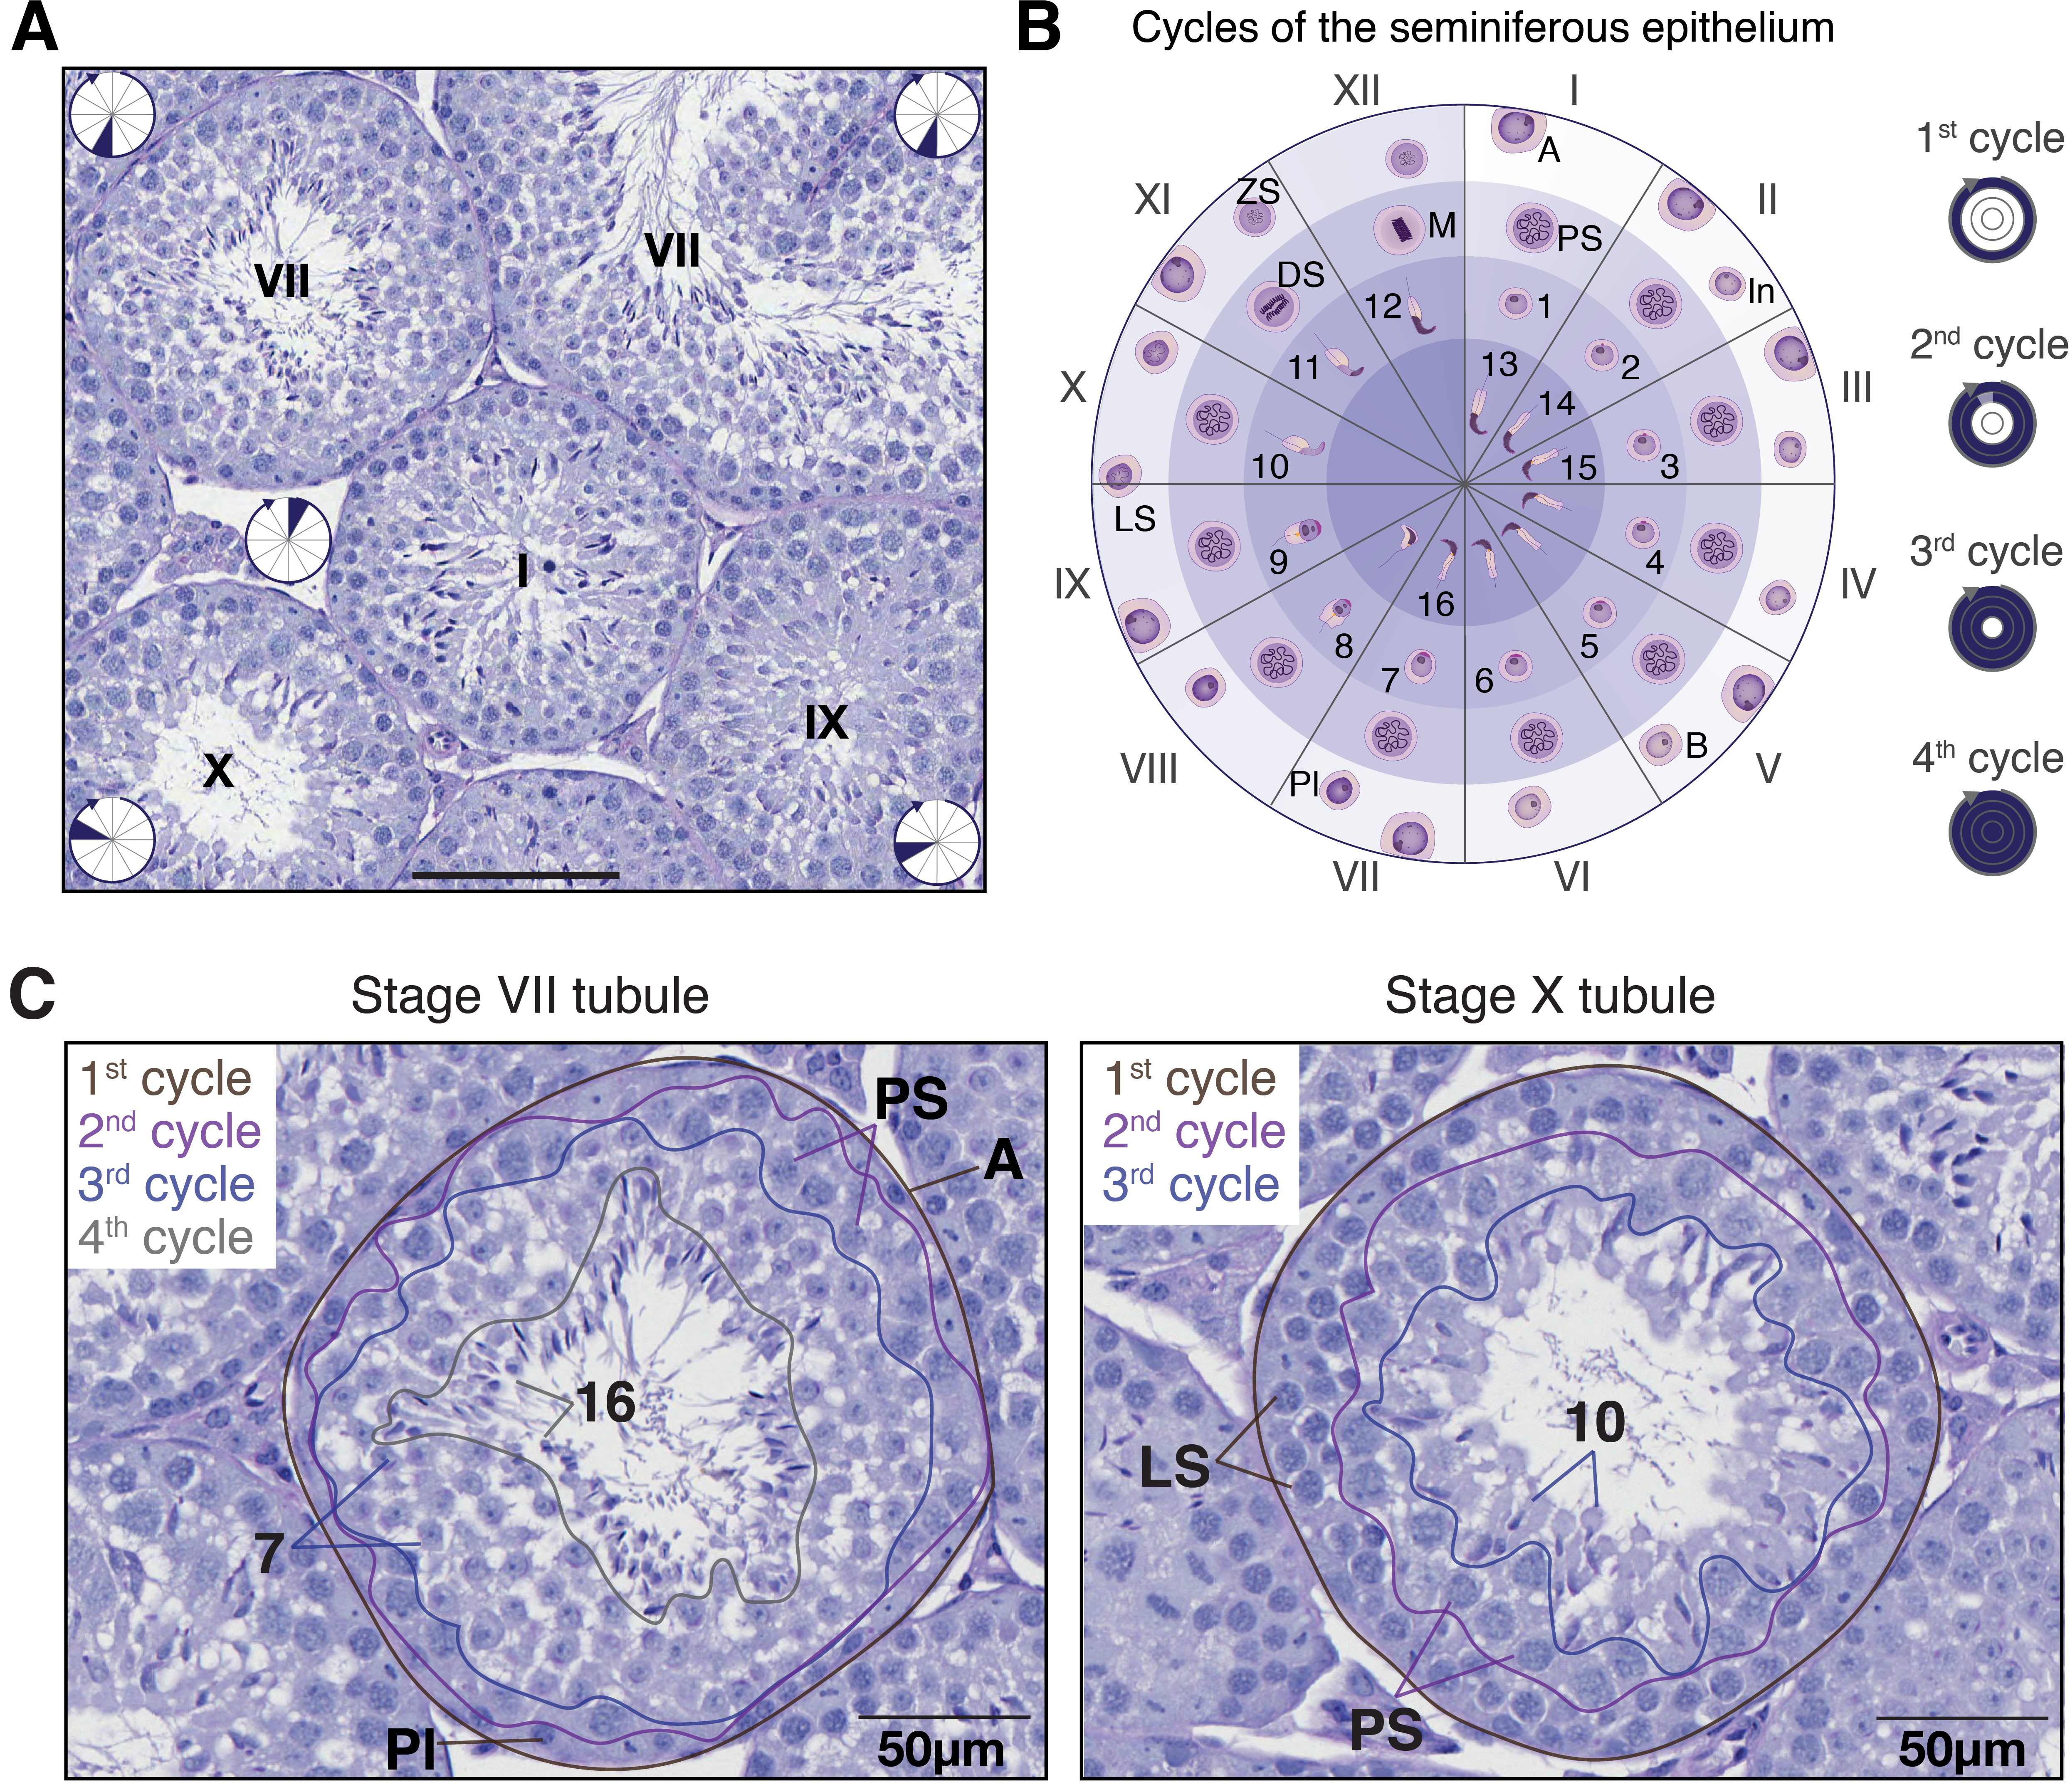
\includegraphics[width=\textwidth]{Fig_1.png}
\caption[Bet-hedging strategy of the $\lambda$-phage]{\textbf{Bet-hedging strategy of the $\lambda$-phage.}\\
The linear genome of the $\lambda$-phage enters the \Gls{Ecoli} host cell and circularises. 
A stochastic decision is made to enter the (i) lytic or (ii) lysogenic cycle where (i) the $\lambda$-phage genome replicates, the $\lambda$-phage particles assemble in the host cell and the cell is destroyed releasing the virions or (ii) the $\lambda$-phage is integrated into the host genome (prophage) and transferred to daughter cells during cell divisions. 
Under stress conditions, the $\lambda$-phage genome is excised from the host genome and enters the lytic cycle.}
\label{fig0:bedhedging}
\end{figure}

In unicellular organisms, \cor{biological noise has been linked to ‘bet-hedging’ strategies, where a sub-optimal fitness landscape is tolerated across a population of cells in order to facilitate an effective response to environmental changes.}. Here, phenotypic heterogeneity facilitates the commitment to alternative cell states in cases of stress (e.g.~nutrient deprivation, temperature fluctuations). 
For example, \Gls{Bsubtilis} either commits to sporulation or competence upon starvation or DNA damage. 
Sporulation describes an irreversible process during which vegetative growth ends and the cell forms endospores that survive the altered environment. 
Competent bacteria on the other hand take up DNA from endospores to repair DNA damage \citep{Schultz2009}. 
The probabilistic and transient activation of competence in a sub-population of \Gls{Bsubtilis} cells is modulated by fluctuations in the competence regulators ComK and ComS. 
An excitable system of negative and positive feedback loops controls the number of cells that reversibly commit to competence while other cells irreversibly execute sporulation \citep{Suel2006}. 
\cor{Variations} in the process of transferring phoshporyl groups across a cascade of regulators maintains a constant probability for cells committing to sporulation under nutrient deprived conditions \citep{Russell2017}. 
A similar phenomenon is observed in \Gls{Ecoli} populations exposed to antibiotics where pre-existing phenotypic heterogeneity allows some cells to resist antibiotic treatment. 
Once regrown, these cells remain sensitive to the antibiotic \citep{Balaban2004}. \\

Similar to phenotypic heterogeneity in unicellular prokaryotes, transcriptional noise facilitates the switching between mating phenotypes in yeast upon exposure to pheromones \citep{Paliwal2007}. 
Comparably, commitment to utilising galactose as a nutrient source is a cell fate transition, which is facilitated by stochastic gene expression \cite{Acar2008}. \\

\cor{In these systems, biological noise introduces variation in mRNA and proteins that increase plasticity for cells to adapt to changeing environments.
However, to control and balance the number of cells that commit to a specific fate, noise needs to be buffered as observed in the regulatory network of feedback loops controlling sporulation and competence.}

\subsection{Development and differentiation}

Similar to bet-hedging strategies in unicellular organisms, noise can facilitate the switch between cell states and the probabilistic induction of differentiation processes \citep{Eldar2010, Chang2008}.
\cor{However, as mentioned above, measuring biological noise in differentiating multi-cellular organisms is challenging and the observed molecular phenotypic variability is a combination of stochastic and deterministic components.} 
It has been shown that transcriptional \cor{variability} increases throughout differentiation \citep{Stumpf2017} and development \citep{Antolovic2017}. 
Dissecting differentiation processes of haematopoietic progenitor cells revealed an increase in transcriptional \cor{variability} directly before cell fate decisions are made \citep{Mojtahedi2016, Richard2016}. 
Once committed, differentiating cell populations collapse in variability and move towards a new attractor state. 
\cor{These studies highlight a possible contribution of molecular variability to cell fate decision event.
However, the observed change in variability within differentiating cell populations is purely correlative and it is not possible, with these experiments, to differentiate between variability causing differentiation or differentiation causing variability.}\\

Studies of recent years proposed that stochasticity in expression \cor{contributes to} early (pre-implantation) embryonic development, and to gastrulation \citep{Dietrich2007}. 
As early as the 4-cell stage embryo, targets of master pluripotency factors Oct4 and Sox2 are heterogeneously expressed \textbf{(Fig.~\ref{fig0:noise_development}, left panel)}. 
This is caused by heterogeneous methylation patterns of \gls{H3R26} induced by \gls{Carm1}, which in turn facilitates the binding of Oct4 and Sox2 to induce pluripotency. 
Cells with unmethylated H3R26 differentiate towards the extra-embryonic trophoectoderm while pluripotent cells form the inner cell mass \citep{Goolam2016}. 
Once the cells compact at \gls{E} 3.5, cells of the \gls{ICM} stochastically express genes to initiate heterogeneity within the cell population \textbf{(Fig.~\ref{fig0:noise_development}, 2\textsuperscript{nd} panel)}. 
Fgf4 driven signal reinforcement controls this heterogeneity to form a salt-and-pepper like cell state pattern at E3.5. 
Positional information and the establishment of gene regulatory networks facilitate the segregation of the epiblast and primitive endoderm lineage at E4.5 \textbf{(Fig.~\ref{fig0:noise_development}, 3\textsuperscript{rd} panel)} \citep{Ohnishi2014}. 
In line with this, scRNA-Seq revealed high levels of \cor{transcriptional variability} in the uncommitted inner cell mass at E3.5 (64-cell stage) in comparison to the E4.5 committed epiblast. 
\cor{Transcriptional variability} increases again upon exit from pluripotency in the E6.5 epiblast while cells of the primitive streak at E6.5 synchronise their expression patterns and \cor{variability} is reduced \textbf{(Fig.~\ref{fig0:noise_development}, right panel)} \citep{Mohammed2017}. \\

\cor{Besides the hypothesis of transcriptional variation contributing to embryonic development, a number of alternative drivers for cell fate decisions the mouse embryo exist\citep{Zhang2018a}. 
For example, in the 8-cell to 16-cell stage embryo, symmetry breaking could be achieved by an interaction between the cell’s position and polarity, its cortical tension, and the orientation of cell division97. 
Maître \emph{et al.} proposed a system where robust self-organization of 8- to 16-cell stage embryos is achieved by differences in contractility between polar and apolar cells, which leads to the internalization of the more contractile apolar cells\citep{Maitre2016}. 
Taken together, it is unclear to which fraction transcriptional variability plays a role in cell fate decision-making and if purely the occurrence of differentiating cells induces transcriptional variation. }

\begin{figure}[!h]
\centering
\includegraphics[width=\textwidth]{Fig_2.png}
\caption[Progression of transcriptional heterogeneity during embryonic development]{\textbf{Progression of transcriptional noise during embryonic development}.\\
From left to right: schematic of mouse embryonic development from the 4-cell stage to early gastrulation at E6.5. 
Cell colours indicate gene expression strength. Variable expression at the 4-cell stage induce commitment to form extra-embryonic lineages or pluripotent cells. 
These pluripotent cells at E3.5 show high expression variability forming the inner cell mass (ICM). 
Cells rearrange to form the epiblast and primitive endoderm at E4.5 while noise levels increase in the epiblast at E6.5 compared to the primitive streak.}
\label{fig0:noise_development}
\end{figure}

While pluripotent stem cells in the mouse embryo commit irreversibly to cell lineages during development, \emph{in vitro} cultured \glspl{mESC} reside in a self-renewing, metastable state \citep{Hayashi2008} and heterogenity within the cell population depends on the growth condition. 
Transcription factor heterogeneity, especially of the pluripotency regulator Nanog, is highest in \gls{LIF}/serum grown cells and allows the Nanog-negative cells to commit to differentiation \citep{Chickarmane2012, Torres-Padilla2014}. 
Heterogeneously expressed genes that show a bimodal distribution in expression counts correlate with each other indicative of the presence of distinct states in mESCs. 
These distinct states show differences in promoter methylation patterns, introducing the role of epigenetic modifications to maintain heterogeneity in mESCs \citep{Singer2014}. 
In-depth analysis of mESCs grown in different media (serum, \gls{2i} and \gls{a2i}) shows the presence of three distinct cell states in the serum grown cells. 
mESCs grown in 2i media show less variability in pluripotency markers but higher heterogeneity in cell cycle related genes \citep{Kolodziejczyk2015cell}. 
From the pluripotent ground state, mESCs can differentiate along somatic lineages via specific differentiation events or noise-induced transitions between attractor states. 
Mathematical modelling has shown that mESCs differentiate stochastically through distinct hidden cell (micro-)states within a defined (macro-)state coupled to an increase in variability \cite{Stumpf2017}.
In contrast to the beneficial features of noise in stem cell differentiation, stochastic events during \gls{iPSC} reprogramming limit the formation of single iPSCs \citep{Hanna2009, Yamanaka2009}. 
It has been shown that probabilistic events dominate in an early phase of reprogramming while the transcription of \textit{Sox2} induces a later, more deterministic, phase \cite{Buganim2012}.\\

\cor{These findings indicate an intrinsic heterogeneity of pluripotent cell populations. 
Extrinsic cues, such as growth medium or signalling networks in the embryo, are needed to control this heterogeneity.
However, it is not clear if this seemingly random expression of pluripotent marker genes is truely stochastic or driven by unobserved regulatory mechanisms.
Hoppe \emph{et al.} challenged the idea of lineage choice by stochastic fluctuations of lineage-specific transcription factors and highlighted, using time-resolved measurements, that these transcription factors are solely reinforcing lineage choice \cite{Hoppe2016}.
Therefore, lineage choice can be initiated by unobserved cues that induce variation in genes expression.} 

\subsection{Stochasticity in immune responses}

Fast and flexible immune responses are only possible within cell populations that show high plasticity and react to a broad spectrum of stimuli. 
Stochasticity in cytokine expression \cor{can} lead to phenotypic variability in the \Gls{Th} cell repertoire and increases the effectiveness to respond upon immune stimuli \citep{Schrom2017}. 
For example, fluctuating expression of the lineage defining cytokines \gls{Ifn}\textgamma{} for Th1 and \gls{Il} 4 for Th2 in small populations of cells drive the cell population towards a Th1 or Th2 cell fate while most cells co-express the lineage defining transcription factors \Gls{Gata} 3 and \Gls{Tbx21} \citep{Fang2013a, Antebi2013}.\\

Furthermore, Shalek \textit{et al.}, 2014 have shown that upon \gls{LPS} stimulation a small subset of dendritic cells become activated much earlier than the rest of the cell population while expressing \gls{Ifn}\textbeta. 
These early responders support the activation of late responding cells via cell-to-cell communication (paracrine signalling) and self-stimulation via autocrine signalling \textbf{(Fig.~\ref{fig0:noise_immune})} \citep{Shalek2014}. 
Likewise, a bimodal (digital) expression of Il2 is detected in \gls{Th} cells after immunisation where the number of Il2 expressing cells scales with antigen level. 
Il2 expressing cells support the activation of surrounding cells via paracrine signalling \citep{Fuhrmann2016}. 
Similarly, digital activation processes can be observed in the \gls{NFkB} signalling pathway. 
The fraction of cells that activate this signalling pathway increase with LPS concentration to avoid strong immune activation at low concentrations of a stimulus \citep{Kellogg2015b}. \\

\cor{While the plasticity and reactivity of immune cell populations is finely tuned by introducing phenotypic heterogeneity, it is not understood how individual cells commit to each phenotype. 
In part, stochastic expression introduces molecular phenotypic variability that in turn is tightly controlled by external and internal signalling networks. 
It will therefore be crucial to study the behaviour of immune cells while incorporating their spatial location which might allow the prediction of each cell's phenotype\cite{Battich2015}.}

\begin{figure}[!h]
\centering
\includegraphics[width=\textwidth]{Fig_3.png}
\caption[Early responders are important for homogeneous immune activation]{\textbf{Early responders are important for homogeneous immune activation.}\\
Within a population of immune cells (e.g.~\gls{DC}, \gls{Th} cells), a sub-population either show higher response strength or induce the production of cytokines such as \gls{Il}2 or \gls{Ifn}\textbeta. 
These early responders induce activation of surrounding cells via paracrine signalling and self-stimulation via autocrine signalling.}
\label{fig0:noise_immune}
\end{figure}

\vspace{-5mm}

\subsection{Tissue development and homeostasis}

Coping with the influence of biological noise is important for regulated tissue development and homeostasis. 
An early study showed that in order to minimise the effect of stochasticity in development, plants express heat-shock protein 90 to stabilise regulators of growth and development \citep{Queitsch2002}. 
Furthermore, redundancy in the \Gls{Celegans} intestinal gene regulatory network buffers variability in the down-stream master regulator \textit{elt-2}. 
Once highly connected regulators of this network are removed, phenotypic variation arises from bimodal expression of \textit{elt-2} \citep{Raj2010}. 
The cooperation of positive and negative feedback loops in these highly connected regulatory networks ensure robust expression of key developmental genes \citep{Ji2013}. 
Other models have been proposed in which noise helps to form sharp boundaries between neighbouring domains \citep{Zhang2012}. 
Contact based adhesion and repulsion between cells sharpens narrow transition regions by sorting cells within a tissue across small scales. 
Noise-driven cell state plasticity on the other hand allows cells to switch states and therefore helps narrow a wider transition region \citep{Wang2017}. 
The plasticity to migrate within a population of cells also allow the correction of sensing errors. 
These errors are induced by either too strong or too weak responses of individual cells to a signalling gradient \citep{Camley2017}.\\

While the cell division rate within tissues is higher during development, tissue homeostasis is maintained by stochastic events that balance cell division and apoptosis \citep{Ranft2010}. 
The effect of noise on maintaining tissue homeostasis has been studied in a diverse set of organs. 
In fat tissue, a complex system of signalling feedback loops controls protein abundance noise to induce differentiation at a low rate but prevents stochastic de-differentiation \citep{Ahrends2014}. 
To maintain coordination in liver function, longer mRNA lifetimes of bursty genes and polyploidy reduce noise in gene expression \citep{BaharHalpern2015}. 
Another mechanism to achieve tissue-wide expression responses involves spatial coordination of stochastically expressing cells in the pituitary gland \citep{Featherstone2016}. 
Spatially constrained signalling events have also been demonstrated to play a role in maintaining colonic crypt cell type diversity. 
Per crypt, eight stem cells differentiate into a defined ratio of cell types. To reduce noise in this process, lateral inhibition within a commitment zone reduces the number of differentiated goblet cells and following slower dispersive migration as well as decreased division rates of goblet cells ensures a distinct 1:3 ratio to enterocytes across all crypts \textbf{(Fig.~\ref{fig0:noise_tissue})} \citep{Toth2017}.

\cor{In sum, phenotypic heterogeneity in tissues can arise from stochastic expression driven by noise.
To control for correct tissue responses, signalling networks are in place to modulate this variation. 
In most studies, individual signalling networks and few molecular read-outs were chosen to understand the variation observed within tissues.
However, a combination of multiple regulatory signalling events control cell fate within tissues and disentangling the individual components has not been feasible.}

\begin{figure}[!h]
\centering
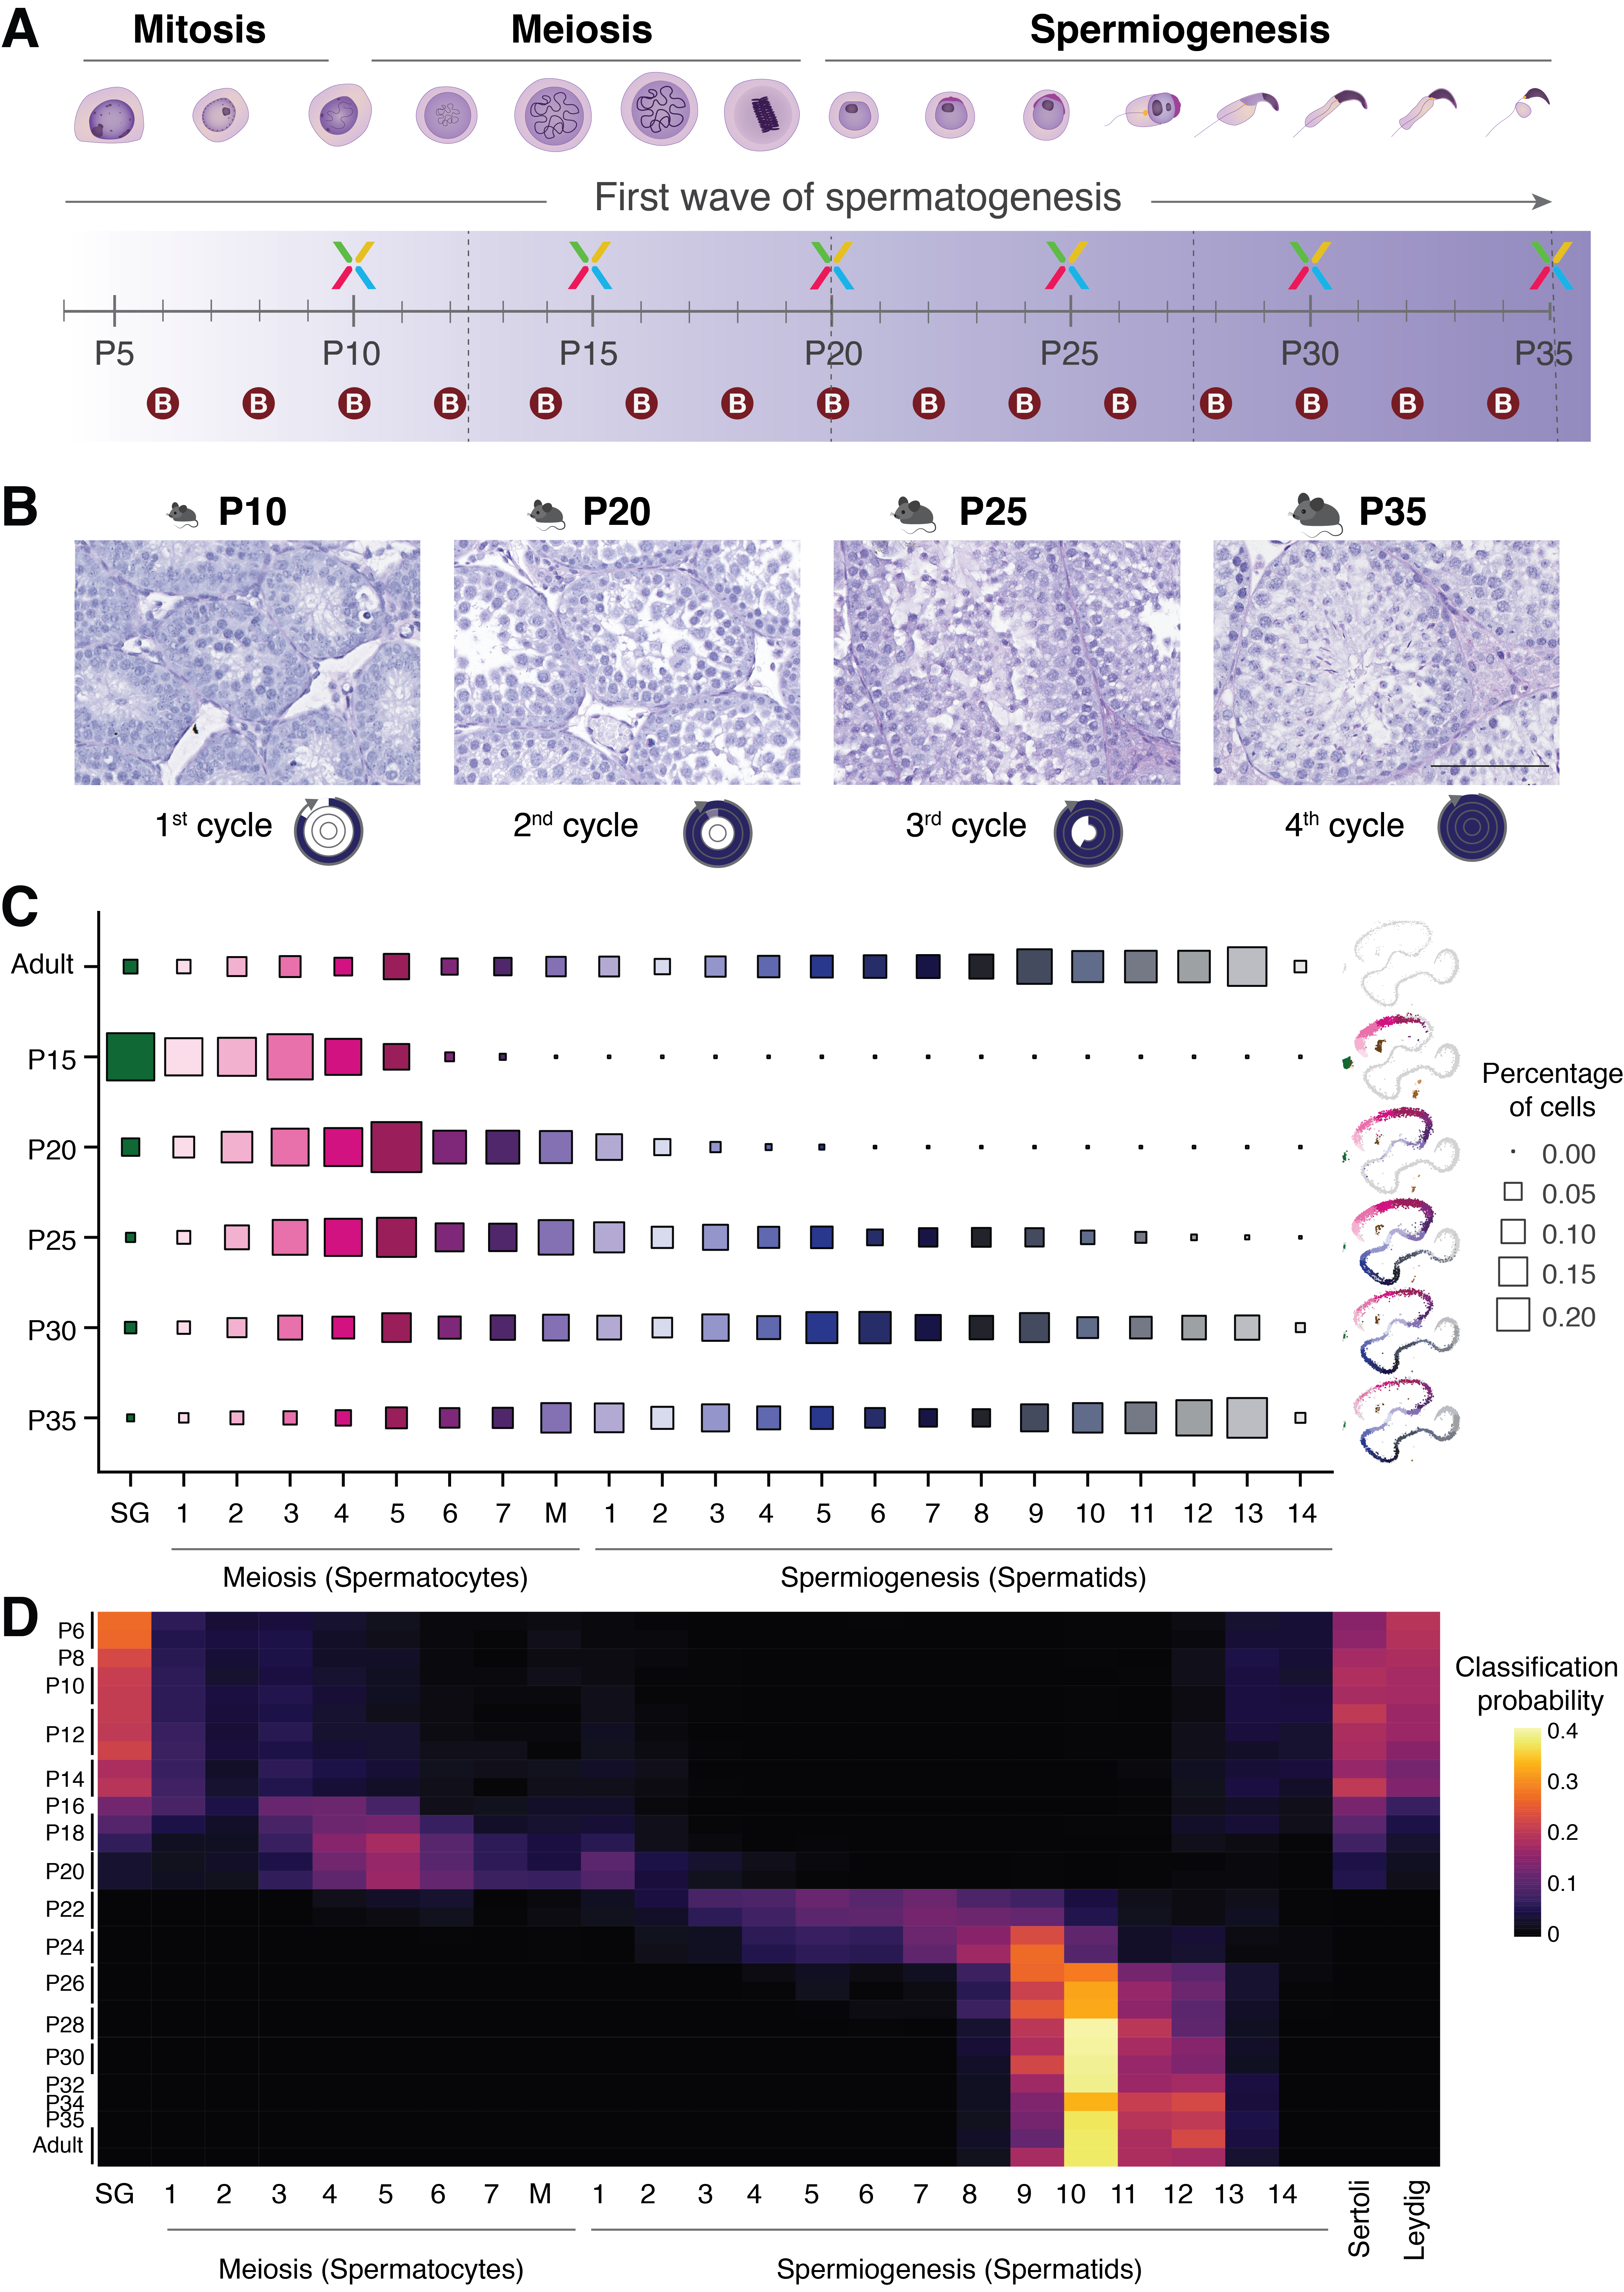
\includegraphics[width=\textwidth]{Fig_4.png}
\caption[Buffering of noise in the colonic crypt]{\textbf{Buffering of noise in the colonic crypt.}\\
Each colonic crypt harbours 6-8 stem cells that divide to form stem cells and progenitors cells. 
Early commitment of progenitor cells to cell fates (e.g.~goblet cells or enterocytes) leads to crypt-to-crypt heterogeneity due to commitment noise (left panel). 
Lateral inhibition within a restricted zone (commitment zone) allows cell fate switching and therefore buffers the crypt-to-crypt heterogeneity (middle panel). 
Migration of goblet cells after the commitment zone buffers the stochastic occurrence of goblet cell or enteroctye patches within the crypt and allows a constant ratio of 1:3 goblet cells to enterocytes in each crypt (right panel). 
Adapted from \citep{Toth2017}.}
\label{fig0:noise_tissue}
\end{figure}

\subsection{Evolution}

As discussed above, biological noise \cor{can be} beneficial for cell fate commitment \cor{but} needs to be \cor{controlled} to allow coordinated expression in cell populations. 
During evolution, a trade-off between cellular plasticity, the expression responsiveness during environmental changes, and robust expression formed. 
Natural selection acts on genetically controlled expansions of quantitative phenotypes, which\cor{, in part, are} derived from biological noise \citep{Eldar2010}. 
For example, \cor{variable} expression of stress response genes allows a cell population to adapt to changing environments \citep{Lopez-Maury2009}. 
Specifically, the expression of genes controlled by TATA-box containing promoters shows strong divergence between species \citep{Tirosh2006}. 
To control for robust expression levels once selection becomes stabilising, noise levels are reduced \citep{Lopez-Maury2009, Eldar2010, Pires2016}. \\

Lehner, 2008 discussed specifically evolutionary selection to minimise noise in genes that show harmful phenotypic effects upon alteration ("dosage-sensitive genes"). 
These genes show low expression \cor{variability} to reduce the probability of altered expression and also lower expression divergence between species \citep{Lehner2008}. 
Furthermore, essential genes tend to cluster in the genome in regions with persistent open chromatin to reduce \cor{the effect of} noise \citep{Batada2007}. 
In line with this, the promoters of core cellular components show a decoupling between expression plasticity and expression \cor{variability}, which indicates that responsiveness in expression is not a general attribute of high expression \cor{variability} \citep{Lehner2010a}. \\

In unicellular populations, \cor{it has been proposed that the contribution of noise on molecular phenotypic variability} evolutionarily increased as a form of rudimentary regulation \citep{Wolf2015}. 
As a consequence, phenotypic heterogeneity increases the adaption rate of cell populations to extreme environments \cite{Bodi2017}. 
Conversely, in multicellular organisms, collections of cells need to respond in a coordinated manner. 
It has therefore been proposed that nuclear compartmentalisation in higher organisms reduces noise by mRNA retention at the nuclear membrane \citep{Battich2013, Stoeger2016}.

\cor{In most cases, cells in an unperturbed state have been profiled to decipher evolutionary selection acting on variability in gene expression.
However, in fluctuating environments where the averaged protein abundance across a cell population is far from the optimum, variability in expression leads to some cells expressing protein levels closer to the optimum. 
By contrast, in stable environments, noise in gene expression can be deleterious by leading to suboptimal growth conditions for many cells\cite{Schmiedel2018,Duveau2018}.
It is therefore crucial to discuss the fitness effect of changes in molecular variability in the context of fluctuating as well as stable environments.}

\subsection{Cancer}

While biological noise \cor{can contributeto } the adjustment of cells to new microenvironments, errors in the form of gene mutations induce transitions from healthy cells towards a cancer attractor state \textbf{(Fig.~\ref{fig0:cancer})} \citep{Marusyk2012}. 
Non-genetic heterogeneity supports the phenotypic adaptation to the new attractor state \citep{Jia2017}. 
The emergence of non-genetic heterogeneity in tumours is coupled to epigenetic dysregulation that allows the survival of cancer cells \citep{Timp2013}. 
Furthermore, it has been proposed that genome wide intra-sample methylation heterogeneity is increased in chronic lymphoitic leukemia increasing cancer cell plasticity in the search for new attractor states \citep{Landau2014}. 
Increased variability in expression can also be observed for more aggressive cancer sub-types across multiple patients \citep{Ecker2015}. \\

An important consequence of \cor{increased} phenotypic heterogeneity in cancer cells is the fractional killing of cell populations upon drug treatment \textbf{(Fig.~\ref{fig0:cancer})} \citep{Flusberg2015}. 
\cor{Variability} in proteins mediating \Gls{TRAIL} induced apoptosis leads to the survival of small fractions of cells \citep{Spencer2009}, which could consequently repopulate the tumour environment. 
Similarly, the stochastic acquisition of DNA damage upon cisplatin exposure introduces heterogeneity in the up-regulation of p53. 
Slow up-regulation leads to cell cycle arrest and inhibits apoptosis while only fast up-regulation leads to cell death \citep{Paek2016}. 
In patient derived melanoma cells, sporadic expression of resistance markers forms a rare cell population that grows into resistant colonies after treatment. 
While pre-resistant cells do not display epigenetic marks and are therefore close to the non-resistant ground state, treatment induces large epigenetic reprogramming, forming stable resistant cancer colonies \citep{Shaffer2017}. 
To tackle this problem, combinatorial therapies have been proposed to reduce variability and fractional killing in cancer cell populations \cite{Paek2016, Roux2015}.\\

\cor{These studies propose a contribution of non-genetic heterogeneity, potentially induced by the loss of noise control, to cancer onset and inefficient treatment response.
However, cancer is a heterogeneous disease that develops in a multi-step process involving disregulation in various cellular systems. 
Therefore, and similar to molecular phenotypic variability in embryonic development, the observed non-genetic heterogeneity can be a phenotypic consequence rather than a driver for cancer onset. }

\begin{figure}[!h]
\centering
\includegraphics[width=\textwidth]{Fig_5.png}
\caption[Heterogeneous cell states and cell responses in cancer development]{\textbf{Heterogeneous cell states and cell responses in cancer development.}\\
Stochasticity in expression introduces non-genetic heterogeneity that supports the adaptation of cancerous cells. 
Cancer progresses to form a collection of cells with divergent expression patterns. 
This phenotypic heterogeneity leads to fractional killing during treatment and cancer recurrence.}
\label{fig0:cancer}
\end{figure}

\newpage

\subsection{Ageing}

Similarly to the onset of cancer, destructive roles of biological noise have been reported during organismal ageing. 
Previously, it has been debated whether expression noise changes during the lifespan of animals \cite{Bahar2006, Warren2007}. 
While these initial studies only used small panels of genes, transcriptional profiling of single cells led to the discovery of a destabilised immune activation programme in CD4\plus{} T cells due to increased expression noise \cite{Martinez-jimenez2017}. 
Similarly, transcriptional noise increases with age in human pancreas coupled to an increased stress signature and atypical hormone expression \citep{Enge2017}. 
For further discussion of age-related effects on transcriptional noise, see \textbf{Chapter 2}. \\


\begin{table}[hb	]
\centering
\caption{Positive and negative effects of biological noise on cellular systems.}
\label{table:effects_noise}
\begin{tabular}{l l l}
\toprule
\toprule
\textbf{System} & \textbf{Friend} & \textbf{Foe} \\ 
\midrule
\midrule
Unicellular organism & Bet-hedging & \\
\midrule
Development and & Probabilistic induction  & \\
differentiation & of cell differentiation & \\
\midrule
Immune response & Plasticity in immune response & \\
 & Control of response strength &   \\
\midrule
Tissue development  & Low cell differentiation rate & Non-uniform development \\ 
and homeostasis &  & Uncontrolled tissue response \\
\midrule
Evolution & Adjustment to  & Non-uniform, stabilising expression \\ 
& fluctuating environment & Uncontrolled tissue responses \\
\midrule
Cancer &  & Phenotypic adaption to cancer state \\
& & Fractional killing of cancer cells \\
\midrule
Ageing &  & Unsynchronised immune response \\
& & Increased stress signatures \\ 
\bottomrule
\bottomrule
\end{tabular}
\end{table}

%!TEX root = ../intro.tex
%******************************
%	 Sources of expression noise
%*****************************

\section{Sources of expression noise} 

\cor{Molecular phenotypic variability} across homogeneous populations of cells \cor{can arise} from intrinsic and extrinsic noise, \cor{and deterministic components} (see \textbf{Box 1} on page \pageref{box1}). 
While intrinsic noise is promoter-specific and therefore induces uncoordinated variation in RNA or protein expression between individual genes, extrinsic noise globally influences gene expression across multiple cells and therefore leads to co-variation across larger sets of genes. 
Here, I give an overview on the different sources of intrinsic and extrinsic noise in a variety of biological systems.

\subsection{Intrinsic noise}

Intrinsic noise in cell populations arises from stochasticity in biochemical reactions that lead to the synthesis of mRNAs (transcription) and proteins (translation) within individual cells. 
Regulatory features on the genomic, epigenetic, transcriptional and translational level influence \cor{and control} the strength of intrinsic noise (for an overview see \textbf{Fig.~\ref{fig0:overview_intrinsic}}).

\begin{figure}[!h]
\centering
\includegraphics[width=0.9\textwidth]{Fig_6.png}
\caption[Regulatory features that modulate expression noise]{\textbf{Regulatory features that modulate expression noise.}\\
Promoter sequence, number of transcription factor (TF) binding sites (TFBS), number of transcriptional start sites (TSS), enhancer elements, RNA polymerase II (RNAPII) loading, DNA methylation, nucleosome positioning, histone modifications, polycomb repressive complex binding, \glspl{miRNA}, nuclear export of mRNA, ribosome binding and blockage via stem loop formation are features that induce gene-specific intrinsic noise.}
\label{fig0:overview_intrinsic}
\end{figure}

\subsubsection{DNA features}

One of the key regulatory steps prior to RNA synthesis is the binding of \glspl{TF} to specific DNA sequences within the regulatory region (promoter) of a gene which then triggers the controlled production of primary RNA transcripts from the DNA of this gene \citep{Latchman1997}. 
Mutations in the DNA sequence such as \glspl{SNV} can alter the binding affinity of TFs and therefore the rate at which a gene is expressed \textbf{(Fig.~\ref{fig0:DNA_features})}. 
A systematic study of the \gls{TDH3} gene expression in yeast found that mutations in known \glspl{TFBS} decrease mean expression and increase expression noise. 
Moreover, Metzger \textit{et al.}, 2015 \cor{proposed} that evolutionary selection removes mutations that increase expression noise and that SNVs with large effects on expression noise show the lowest frequency within sampled yeast strains \citep{Metzger2015}. 
\cor{However, the authors examined one promoter in stable environmental conditions. 
How selection on mutations that induce variability in expression works in more complex systems and across multiple promoters is still unexplored.}\\

One of the most widely studied DNA motifs in relation to transcriptional noise is the TATA-box motif in promoters. 
Generally, TATA-box containing promoters show high levels of transcriptional noise \textbf{(Fig.~\ref{fig0:DNA_features})} \citep{Faure2017}, possibly due to a simple activation cycle containing one or few inactive states \citep{Zoller2015}. 
Moreover, TATA-box containing genes show an increased interspecies variability \citep{Tirosh2006} and higher spontaneous mutational variation \citep{Landry2007}, indicating an increased evolvability of these particular genes. 
In an early study, Raser \textit{et al.}, 2004 studied the noisy expression controlled by the budding yeast \gls{PHO5} promoter. 
This promoter contains the TATA-box motif and it has been shown that transcriptional noise is reduced when a mutational modification decreases the TATA-box strength \citep{Raser2004}. 
A more recent study confirmed this result and found mutations in yeast promoters that eliminate the TATA-box motif which lead to reduced noise levels for these genes \citep{Hornung2012}. 
\cor{The TATA-box is therefore one genomic feature that can differentiate between genes with variable and stable expression and are enriched amongst stress response genes, which support their role in early adjustment to changing environmental conditions \citep{Lopez-Maury2009}.}\\

\cor{However, a} possible confounding factor for the increased noise of TATA-box containing promoters is the number of TFBSs. 
Tirosh \textit{et al.}, 2006 detected a two-fold enrichment of TFBSs in TATA-box containing promoters \citep{Tirosh2006}. 
A later study showed that transcriptional noise scales with increased numbers of TFBSs \textbf{(Fig.~\ref{fig0:DNA_features})} \citep{Sharon2014}. 
Furthermore, TATA-box containing genes lack enhancing histone marks and their increased variability in expression can therefore be explained by repressed chromatin \citep{Choi2008} (see \textbf{Section \ref{sec0:epigenetic}}).  

\begin{figure}[!h]
\centering
\includegraphics[width=0.9\textwidth]{Fig_7.png}
\caption[Features of the DNA sequence induce expression noise]{\textbf{Features of the DNA sequence induce expression noise.}\\
Mutations of the transcription factor (TF) binding site (TFBS), the presence of a TATA box, increase number of TFBSs, reduced number of transcriptional start sites (TSSs) and reduced copy number of genes can induce transcriptional noise.}
\label{fig0:DNA_features}
\end{figure}

Promoters can be classified based on their shape as narrow, with few \glspl{TSS} that predominantly control tissue-specific gene expression, and broad promoters with larger numbers of TSSs that control the expression of house keeping genes. 
Mutations that alter the shape of promoters increase transcriptional \cor{variability} \citep{Schor2017a}. 
Furthermore, promoters with one or few TSS show higher levels of expression variability \textbf{(Fig.~\ref{fig0:DNA_features})} \citep{Faure2017}.

\newpage

In addition to \glspl{SNV}, \glspl{CNV} (usually defined as copy number variability of regions $\geq$ 1kb in comparison to a reference genome) in parts of the genome influence gene expression and contribute to, for example, schizophrenia and autism \citep{Gamazon2015}. 
Combined analysis of DNA and RNA has shown that genes with low copy number tend to be more noisily expressed compared to genes encoded by multiple copies \textbf{(Fig.~\ref{fig0:DNA_features})} \citep{Dey2015}. 
In the context of monoallelic expression, genes located on the X chromosome show increased mRNA half-life which in turn increases transcript stability and reduces noise to levels of autosomal genes \citep{Faure2017}.\\

\cor{In sum, these findings highlight that multiple correlated genomic features are associated with modulating noise. 
It is therefore challenging to disentangle the individual underlying sources of transcriptional variability. }

\subsubsection{Epigenetic factors}
\label{sec0:epigenetic}

Epigenetic research is defined as "the study of changes in gene function that are mitotically and/or meiotically heritable and that do not entail a change in DNA sequence" \citep{Wu2001}. 
Epigenetic factors are generally described as DNA methylation at \gls{CpG} dinucleotides, histone modifications and nucleosome positioning  \citep{Portela2010}. 
\textbf{Table \ref{tab0:epigenetic}} summarises the relationship between epigenetic features and \cor{variable} gene expression. \\

\Gls{CGI} are genomic sites of more than 200 bases with a GC content of more than 50\% and are usually unmethylated. 
Methylation of CGIs in promoters is linked to gene silencing while DNA methylation in gene bodies facilitates transcription \citep{Portela2010}.  
Recently, the presence of CGIs in gene bodies but also at the TSS and in promoter regions was linked to a reduction in transcriptional \cor{variability} \citep{Faure2017}. 
\cor{Morgan and Marioni, 2018 further distinguished between gene promoters associated with short and long CGIs.  
Similar to the presence of TATA-box motifs as described above, the length of CGIs in promoter regions controls how variably a gene is expressed. 
Genes associated with short CGIs tend to be more variably expressed and allow an early response to stimulation, exemplified by observations in mouse bone-marrow derived dendritic cells and human breast cancer cells \citep{Morgan2018}.
However, it is not clear whether the length of CGIs is the sole driver for variable gene expression or how multiple genomic features work together to induce transcriptional variability.} \\

Modifications of histones induce the \cor{opening} or repression of chromatin and  therefore indirectly modulate gene expression \citep{Suganuma2011}. 
In an extensive study to link histone modifications to transcriptional \cor{variability}, Faure \textit{et al.}, 2017 detected several histone modifications in promoter/core promoter motifs, at the TSS and in gene bodies that increase or decrease \cor{variability}. 
The repressive \gls{H3K27me3} mark is linked to higher \cor{variability} when present at the TSS, in promoters and in gene bodies. 
The enhancer related \gls{H3K4me1} mark only increases \cor{variability} when present at the TSS and in the core promoter sequence while the repressive \gls{H3K9me3} mark increases \cor{variability} when present in the promoter motif. 
The activating marks \gls{H3K4me3}, \gls{H3K9ac} and \gls{H3K36me3} are linked to low levels of \cor{variability} when present in gene bodies. 
In addition to these single features, bivalent promoters that carry the repressive \gls{H3K27me3} and enhancing \gls{H3K4me3} marks show high levels of transcriptional \cor{variability} \citep{Faure2017}.
\cor{Here and in Morgan and Marioni, 2018, the authors profiled molecular phenotypic variability in "homogeneous" populations of \glspl{mESC} as proxy for transcriptional noise.
While the effect of fluctuation in cell-cycle stages was regressed out, unobserved variation in, for example, the differentiation potential of mESCs in serum grown medium \cite{Kolodziejczyk2015cell} could still exist.
It is therefore difficult to use scRNA-Seq data to study the true underlying effect of transcriptional noise on the overall observable phenotypic variability.}\\ 

\cor{One suggestion why bivalent promoters show high transcriptional variability was brought forward by Kar \emph{et al.}, 2017.
Here, the authors studied the function of \glspl{PRC} in mESCs.}
PRCs are epigenetic modifiers of histones that repress transcription of developmental genes \citep{Chittock2017} and they can bind together with active \gls{RNAPII} to bivalent promoters. 
Switching between the repressed and active states introduces gene expression variability across a population of cells \cite{Kar2017}.
\cor{However, bulk measures were used to identify the bivalency of promoters.
That leaves the possibility that in a fraction of cells the promoter resides in an open state while in other cells the promoter is repressed. 
This highlights the fact that bulk measures might not be suitable to obtain a correct measure of promoter states in cell populations that could contain unobserved cell state heterogeneity.} \\

Chromatin is the packaged state of DNA within the nucleus and its central elements are nucleosomes. 
Nucleosomes are combinations of eight of the four histones (H3, H4, H2A, H2B) around which 147 bases of DNA twist. 
An array of histone modifying enzymes exist that regulate the opening or closing of the chromatin; termed heterochromatin and euchromatin, respectively \citep{Kouzarides2007}. 
Tirosh \textit{et al.}, 2008 showed that promoters with high nucleosome occupancy close to the TSS tend to display a high range of expression levels across varying conditions (transcriptional plasticity). 
Distant nucleosome-rich regions are on the other hand associated with low transcriptional \cor{variability} \citep{Tirosh2008}. 
Nucleosome covered promoters display shorter transcriptional rates, which in turn explains increased transcriptional \cor{variability} for these promoters \cite{Dey2015}. 
Single-cell measures indicate cell-to-cell variations in nucleosome positioning around the \textit{PHO5} promoter upon stress induction. 
Even in the non-stressed state, a small fraction of cells exhibit nucleosome free regions at the promoter which explains low and possibly noisy expression of \textit{PHO5} \citep{Small2014}.
\cor{This observation again highlights the lack of resolution when using bulk measures to profile the promoter architectures in cell populations.
However, current single-cell technologies to profile epigenetic marks lack throughput and are influenced by high levels of technical noise.
The observed variations in nucleosome occupancy could therefore be driven by technical variation.} \\

Boundaries between heterochromatin and euchromatin are controlled by boundary elements, such as the transcription factor \Gls{CTCF}, that recruit chromatin modifying factors \citep{Kouzarides2007}. 
CTCF also regulates transcription by activating or repressing promoters and regulates distant chromatin interactions \citep{Kim2015a}. 
Recent studies suggest that long-range enhancer-promoter interactions modulate transcriptional noise. 
Interference of CTCF-mediated enhancer-promoter contact either by CTCF knock-out or CTCF-binding site deletion leads to increased expression variability in selected genes \citep{Ren2017}. 
\cor{This study however only profiled protein abundance of few genes and did not correct for changes in mean expression that are highly correlated with changes in variance \cite{Brennecke2013}.}
Enhancers are cis-regulatory elements of non-coding DNA containing TFBSs that regulate the expression of neighbouring genes \citep{Blackwood1998}. 
Genes within super-enhancer loci, a region with multiple enhancers, control pluripotency master regulators and show high levels of variability in expression down-stream targets of these master regulators show similar co-variation across mESCs \citep{Faure2017}.

\newpage

\begin{table}[hb	]
\centering
\caption{Epigenetic control of transcriptional noise}
\label{tab0:epigenetic}
\begin{tabular}{l l c c}
\toprule
\toprule
 & Feature & \cor{Variable} & Stable \\ 
\midrule
\midrule
\multirow{3}{*}[-2pt]{DNA methylation} & CGIs &  & \checkmark{} \\
\cmidrule{2-4}
& Short CGIs & \checkmark{} &  \\
\cmidrule{2-4}
& Gene body methylation &  & \checkmark{} \\
\midrule
\multirow{7}{*}[-2pt]{Histone modification} & H3K27me3 (TSS, promoter, gene body) & \checkmark{}  & \\
\cmidrule{2-4}
& H3K4me1 (TSS, promoter) & \checkmark{}  & \\
\cmidrule{2-4}
& H3K9me3 (promoter) & \checkmark{}  & \\
\cmidrule{2-4}
& H3K4me3 (gene bodies) &  & \checkmark{}\\
\cmidrule{2-4}
& H3K9ac (gene bodies) &  & \checkmark{} \\
\cmidrule{2-4}
& H3K36me3 (gene bodies) &  & \checkmark{} \\
\cmidrule{2-4}
& H3K27me3 and H3K4me3 & \checkmark{}  & \\
\midrule
\multirow{3}{*}[-2pt]{Nucleosome position} & Nucleosome rich promoters & \checkmark{} & \\
\cmidrule{2-4}
& Distant nucleosome rich regions &  & \checkmark{} \\
\cmidrule{2-4}
& Deletion of nucleosome remodelling complexes & \checkmark{}  & \\
\midrule
\multirow{7}{*}[-2pt]{Genome architecture} & CTCF knock-out & \checkmark{} & \\
\cmidrule{2-4}
& CTCF binding site depletion & \checkmark{} & \\
\cmidrule{2-4}
& Clustered genes &  & \checkmark{} \\
\cmidrule{2-4}
& Nuclear-lamina associated genes & \checkmark{} & \\
\bottomrule
\bottomrule
\end{tabular}
\end{table} 

Moreover, the positioning of genes on the genome controls expression noise with densely clustered genes being less \cor{variably} expressed in comparison to non-clustered genes \citep{Kustatscher2017}. 
Additionally, genes positioned next to “noisy” genes display higher levels of transcriptional variability compared to genes that are located in proximity to “stable” genes \citep{Kar2017}. 
Expression \cor{variability} is also increased for genes that are located in a repressed neighbourhood, namely active genes in constitutive nuclear lamina-associated domains \citep{Faure2017}.
\cor{This finding again highlights that genes associated with repressed chromatin display higher transcriptional variability compared to genes associated with open chromatin.
Single-cell measures are needed to provide an insight into whether this effect is driven by so called "leaky" expression from closed promoters of if heterogeneous promoter states can be observed.}

\subsubsection{Transcriptional features}

Transcription is initiated by TFs binding to specific regulatory DNA sequences followed by recruitment of RNAPII and RNA synthesis. 
As discussed above, promoter architecture, namely the location and accessibility of TFBS and RNAPII binding sites, dictates mean expression and transcriptional \cor{variability}. \\

In bacteria, the intracellular physical distance between TF source and the promoter sequence influences expression variability. 
TF expression proximal to their target genes results in less \cor{variable} expression compared to TF expression which occurs distant to the promoter sequence \citep{Goni-Moreno2017}. 
Once TFs bind to their target sequence, Carey \emph{et al.}, 2013 showed that the mean expression to \cor{expression variability} ratio is promoter dependent while in the majority of cases, \cor{variability} negatively scales with mean expression \citep{Carey2013}. \\

Similar to TF binding dynamics, the assembly of RNAPII complexes modulates transcriptional noise. 
An early study identified the connection between paused RNAPII and synchronous expression of target genes. 
Genes without pre-loaded RNAPII show more stochastic activation patterns \citep{Boettiger2009}. 
This finding has later been confirmed using scRNA-Seq data where increased variability was detected for genes with actively transcribing RNAPII across the full range of expression levels \textbf{(Fig.~\ref{fig0:RNAPII})} \citep{Day2016}.
\cor{However, genes with pre-loaded RNAPII also have a higher CpG content and are depleted for TATA-box elements \cite{Day2016}. 
Once again, the correlation between genomic factors and their individual associations with variation creates a challenge for disentangling their specific effects on molecular phenotypic variation.
Alternatively, this may also represent multiple regulatory layers that combine to modulate noise. }\\

\begin{figure}[!h]
\centering
\includegraphics[width=0.7\textwidth]{Fig_8.png}
\caption[RNAPII pausing reduces transcriptional noise]{\textbf{RNAPII pausing reduces transcriptional noise.}\\
Left: Pre-loaded RNA polymerase II (RNAPII) allows direct transcription upon transcription factor (TF) binding. 
Right: RNAPII recruitment induces gene expression variability.}
\label{fig0:RNAPII}
\end{figure} 

\newpage

\subsubsection{Post-transcriptional and translational features}

After synthesis, pre-RNAs are polyadenylated and spliced to form mRNA that relocates from the nucleus to the cytoplasm where translation occurs to synthesise proteins \cite{Glisovic2008}. 
On the post-transcriptional and translational level, mRNA location, structure, degradation and translation have been shown to influence cell-to-cell variation in protein abundance.\\

Upon transcriptional activation, RNAs are produced in burst-like patterns where burst frequency modulates mean expression and noise, and burst size influences solely mean expression \citep{Hornung2012}. 
While bursty transcript synthesis introduces stochastic fluctuations in nuclei between cells, active export of mRNAs into the cytoplasm can dampen this source of variability \textbf{(Fig.~\ref{fig0:posttranscriptional})} \citep{Battich2015a}. 
Reduced cytoplasmic noise has also been shown for two nuclear-retained genes in the mammalian liver. 
Furthermore, this mode of noise control was proposed to be active across a range of metabolic tissues \cite{BaharHalpern2015a}.

\begin{figure}[!h]
\centering
\includegraphics[width=\textwidth]{Fig_9.png}
\caption[Post-transcriptional regulation to control noisy expression]{\textbf{Post-transcriptional regulation to control noisy expression.}\\
Bursty expression introduces nuclear variation in transcript abundance that is buffered due to retention at the nuclear membrane. Within the cytoplasm, micro RNAs degrade lowly expressed genes to reduce expression noise. 
Deletion of the ribsosome binding site as well as stem loop formation increase variability in protein abundance across cells. 
Arrows indicate either increased (red) or decreased noise (green) depending on the regulatory mechanism.}
\label{fig0:posttranscriptional}
\end{figure} 

\cor{Conversely, a recent study by Hansen \emph{et al.}, 2018 proposed an amplification of transcriptional variability due to nuclear export \cite{Hansen2018}. 
However, the authors computed the Fano factor (variance divided by mean expression) as measure of variability and assumed that its value is not correlated with mean expression. 
This assumption arises from an underlying Poissonian (Fano factor is equal to 1) or over-dispersed Poissonian (Fanor factor is larger than 1) distribution of transcript counts.
In reality, the Fano factor is not constant across the range of mean expression. 
This has been discussed by Gr\"un \emph{et al.}, 2014, who showed scale differences in the coefficient of variation (CV) versus mean expression dependency for lowly and highly expressed genes \cite{Grun2014}.
Hansen \emph{et al.} also showed this effect when plotting the Fano factor versus mean expression.
Across all genes, the cytoplasmic transcript abundance as well as the Fano factor were larger compared to nuclear measures, which is to be expected by the model proposed by Gr\"un \emph{et al.}, 2014.
It is therefore recommended to fit a non-parametric curve to variability measure versus mean expression and compare the regression residuals as explained in Chapter 3.}\\

Within the cytoplasm, mRNAs are subject to translation or degradation. 
At this stage, \cor{variability induced by} bursty gene expression is propagated to form variation in protein abundance. 
The availability of mRNAs for translation is not only dictated by their synthesis but also their degradation rate. 
mRNA degradation is accelerated by recognition of \glspl{miRNA}. 
This process has been shown to preferentially reduce noise levels for lowly expressed genes in mESCs, possibly to retain cellular identity \textbf{(Fig.~\ref{fig0:posttranscriptional})} \citep{Schmiedel2015}. 
\\

In addition to noise introduced by stochastic processes on the transcriptional level, the recognition and binding of ribosomes to mRNAs for translation initiation is a source for variation in protein abundance. 
Modulating translational efficiency by mutating the ribosome binding site and initiation codon showed an association between translation and variation in protein abundance \textbf{(Fig.~\ref{fig0:posttranscriptional})} \citep{Ozbudak2002}. 
Additionally, mRNA secondary structure formed by stem loops and poly(G) motifs affects translation initiation and increases variation in protein levels \textbf{(Fig.~\ref{fig0:posttranscriptional})} \citep{Dacheux2017a}.\\

\cor{Together, these studies again highlight a multitude of factors that can modulate the observable variation in transcript and protein abundance. 
Moving forward, models that correct or account for variations introduced by different factors need to be developed to disentangle the individual sources of molecular variation.}

\newpage

\subsection{Extrinsic noise}

\cor{Classically, extrinsic noise has been described to arise from fluctuations in molecules that affect the global gene expression landscape of the cell \cite{Elowitz2002}.
Measuring extrinsic noise is only possible in bacterial populations that do not show fluctuations in cell states.
Nowadays, extrinsic noise is often described to arises from cells being in different regulatory states.}
Here, differences in cellular components introduce variation in mRNA and protein abundance. 
The presence of cell states in otherwise homogeneous populations is characterised by differences in metabolism, cell cycle, cellular volume, cell-to-cell and environmental signalling as well as cell density. 
It has been shown that extrinsic noise forms a major contribution to variation in gene expression and that transcript distributions can be predicted from the cellular state, population context and microenvironment \citep{Battich2015a}.
\cor{Being able to predict transcript abundance however indicates that extrinsic noise is not purely stochastic but might also contain deterministic components.}

\begin{figure}[!h]
\centering
\includegraphics[width=0.7\textwidth]{Fig_10.png}
\caption[Differences in cell states induce extrinsic noise]{\textbf{Differences in cell states induce extrinsic noise.}\\
Within a homogeneous population of cells (left), individual cells reside in different cellular states (e.g.~cell cycle, cell signalling, metabolism) and show differences in cellular volume.}
\label{fig0:extrinsic}
\end{figure} 

\subsubsection{Cell cycle}

Cell cycle has been widely discussed to form a \cor{major} source of extrinsic noise \citep{Colman-Lerner2005, Newman2006}. 
In yeast populations, differences in transcriptional activities between the G1 and S/G2/M phases of the cell cycle lead to large-scale transcriptional heterogeneity across cell populations \textbf{(Fig.~\ref{fig0:extrinsic})} \citep{Zopf2013}. 
Under nutrient-poor conditions, growth rate is reduced and \cor{transcriptional variability} is elevated due to cells being in different cell cycle stages \citep{Keren2015}. 
Even under optimal growth conditions for mESCs (2i media), cell cycle related genes show strong heterogeneity in expression across the cell population \citep{Kolodziejczyk2015cell}. 
\cor{However, it is possible that unobserved regulatory mechanisms are in place to induce proliferation, which otherwise appears to occur randomly across a population of cells.}
When quantifying cell-to-cell variation, cell cycle induced extrinsic noise is often seen as unwanted variation and can mask more subtle transcriptional heterogeneity. 
Computational methods have been developed to correct for this confounding effect to enhance the underlying signal \citep{Buettner2015, Buettner2017}. 

\subsubsection{Cell volume}

Cellular volume provides another explanation for global differences in mRNA content between individual cells introducing large-scale transcriptional \cor{variability} \textbf{(Fig.~\ref{fig0:extrinsic})}. 
Even though cell volume changes during cell cycle progression, within each phase, cell volume can vary as much as across all phases. 
It has been shown that mRNA counts scale with cellular volume to maintain transcript concentrations within each cell \citep{Kempe2015, Padovan-Merhar2015, Zhurinsky2010}. 
\cor{Again, it is not fully understood how cell volume is controlled across a population of cells; especially within multicellular organisms. 
Therefore, the volume of a cell does not necessarily stochastically but rather deterministically contribute to the observed molecular phenotypic variability.}
To avoid this source of heterogeneity, normalisation approaches correct for differences in mRNA content between individual cells \citep{Vallejos2017}.

\subsubsection{Metabolism}

The effect of metabolic fluctuations has been studied in \textit{E. coli} populations. 
Variations in biochemical reactions are induced by noise in the expression of their corresponding catalytic enzymes. 
Changes in metabolism are then coupled to varying growth rates of individual cells, which in turn introduce large-scale transcriptional heterogeneity in cell populations \textbf{(Fig.~\ref{fig0:extrinsic})} \citep{Kiviet2014}.  

\subsubsection{Expression capacity}

Expression capacity is defined as the ability of a cell to express proteins from a gene by utilising the transcriptional and translational machinery. 
Fluctuations in the expression capacity of cells due to quantitative differences in RNAPII or ribosomes can induce global variability among the majority of proteins \citep{Colman-Lerner2005}.

\newpage

\subsubsection{Cell signalling}

A different source of extrinsic noise is the intra- or inter-cellular signalling state of individual cells. 
Fluctuations in membrane bound or cytoplasmic proteins lead to inconsistent transmission of signalling stimuli as exemplified by variability in \gls{TRAIL}-induced apoptosis \citep{Spencer2009}. 
Similarly, variations of regulators in the \gls{ERK} signalling pathway introduce downstream variability in nuclear response \textbf{(Fig.~\ref{fig0:extrinsic})}. 
The degree to which nuclear ERK response varies depends on the position of the regulator in the topology of the signalling pathway \citep{Iwamoto2016}. 
In \textit{C. elegans}, perturbation of the Wnt signalling pathway displayed different degrees of variability in expression of the key Hox gene for Q neuroblast migration, \textit{mab-5}. 
It has been proposed that extrinsic noise, in this case the strength of the Wnt signal, modulates intrinsic variation in the expression of \textit{mab-5} \citep{Ji2013}. 
\cor{These examples describe a system where noise introduces variation in individual components. 
However, this variation is modulated by signalling networks, which allows the cells to precisely respond to external cues. }

\subsubsection{Physical constraints}

\begin{wrapfigure}{r}{0.5\textwidth}
\centering    
\includegraphics[width=0.48\textwidth]{Fig_11.png}
\caption[Physical constraints induce heterogeneous expression patterns.]{\textbf{Physical constraints induce heterogeneous expression patterns.} \\
Cell density increases during the expansion of a homogeneous population of cell forming patches with high and low density, pushing cells to the edge of the population. 
Based on these physical constraints, cells change their transcriptional programme, inducing variability across the population.}
\label{fig0:constrains}
\end{wrapfigure}

Physical constraints on cell growth and the direct population context influence the state of individual cells \citep{Battich2015a}. 
Snijder \textit{et al.}, 2009 performed detailed imaging based analysis of adherent human cells that were infected with different viruses. 
Clathrin mediated endocytosis was most variable with low cell density leading to inefficient mouse hepatits virus infection. 
Dengue virus preferentially infects edge cells while simian virus 40 infection decreased with large cell density \citep{Snijder2009}. 
These experiments indicate the importance of local cellular microenvironment and cell-cell contacts leading to heterogeneity in cell states \textbf{(Fig.~\ref{fig0:constrains})}. 


%!TEX root = ../intro.tex
%******************************
%	 Quantification of biological noise
%*****************************

\section{Quantification of cell population heterogeneity} 

\cor{In the last ten years, the scale of single-cell assays increased from measuring few to hundreds and thousands of genomic, epigenetic, transcriptomic or proteomic features. These technologies can be used to measure molecular phenotypic variability, as well as gain an understanding of the regulatory features that modulate it. The ability to study noise using technology that destroys the cell is formulated on the basis that a cross-section over a population of cells is representative of the time-resolve noise profile of any given cell\cite{Ozbudak2002}.} 
In this section, I will discuss the applicability of single-cell sequencing and imaging technologies as a potential read-out for cell population heterogeneity induced by transcriptional noise.

\subsection{Single-cell sequencing}

Next generation sequencing approaches have been applied to individual cells to quantify variation in DNA sequence, mRNA expression, epigenetic marks and protein abundance within a cell population. 

\subsubsection{Single-cell whole genome sequencing}

\Gls{scDNA-Seq} has previously been used to identify CNVs and SNVs between single cells \citep{Zong2012}. 
Based on these read-outs, tumour heterogeneity and evolution \citep{Navin2011} as well as lineage relationships in the human brain were inferred \citep{Evrony2015}. 
To obtain enough genomic material, \gls{WGA} is performed on DNA from individual cells. The \gls{SCOMP} degrades DNA via restriction enzymes, includes a primary \gls{PCR} amplification step and a later re-amplification via comparative genomic hybridisation \citep{Klein1999}. \Gls{MDA} is based on the random initiation of amplification via oligonucleotide primers with strand displacement \citep{Dean2002}. Compared to MDA, \gls{MALBAC} achieves an initial quasi-linear amplification step by pre-amplification using primers with handle sequences. 
Full amplicons form hairpins that are exponentially amplified prior to sequencing \citep{Zong2012}. \\

The main limitation of single-cell DNA sequencing is the genomic coverage per cell. 
While the detection of SNVs requires deep sequencing of individual cells, CNVs can be detected with shallow sequencing therefore allowing the throughput to increase \textbf{(Fig.~\ref{fig0:scDNA-Seq})} \citep{Knouse2016, Baslan2015}. 
Recently, Vitak \emph{et al.}, 2017 introduced \gls{sci-Seq} which allows the generation of thousands of single-cell genomes for sequencing. 
In the first step, multiple nuclei are sorted into each well of a 96 well plate and the genomic DNA is labelled with barcodes by transposase tagging. 
In the second step, 15-25 tagged cells are sorted into individual wells of a PCR plate where the second round of barcoding is performed during amplification. In that way, CNVs of over 15,000 cells can be assessed \citep{Vitak2017}.
\cor{While previously only bulk measures have been used to link mutations to changes in transcriptional variations\cite{Metzger2015}, scDNA-Seq with high read-depth can be used to solve the question of whether the same mutation in each cell (germ line mutation) or a heterogeneous mutational pattern (somatic mutation) causes the observed increase/decrease in phenotypic variability.}

\begin{figure}[!h]
\centering
\includegraphics[width=\textwidth]{Fig_12.png}
\caption[ScDNA-Seq allows detection of SNVs and CNVs between individual cells]{\textbf{ScDNA-Seq allows detection of SNVs and CNVs between individual cells.}\\
Individual nuclei are captured in 96-well plates and directly lysed or fixated for multiplexing. Whole genome amplification (WGA) can be performed using MDA, MALBAC or SCOMP resulting in amplified genome segments. 
Depending on the biological question, whole genomes are either sequenced thoroughly to detect single nucleotide variants (SNVs) while shallow sequencing can be used to detect copy number variations (CNVs).}
\label{fig0:scDNA-Seq}
\end{figure}

\vspace{-5mm}

\subsubsection{Single-cell RNA sequencing}

Initial approaches to quantify mRNA abundance within single cells included targeted microfluidic-based single-cell \gls{RT-PCR} \citep{Warren2006} and whole-transcriptome read-outs of hand-picked cells \citep{Tang2009}. 
Methods for cell capture range from micromanipulation \citep{Grindberg2014} and laser capture microdissection \citep{Frumkin2008} as targeted methods with low throughput to  \gls{FACS} \citep{Hayashi2010, Dalerba2011, Jaitin2014}, microfluidics \citep{Trapnell2014, Treutlein2014} and microdroplets \citep{Klein2015, Macosko2015} as high-throughput approaches \textbf{(Fig.~\ref{fig0:scRNA-Seq})}. 
More broadly, microfluidic-based \gls{scRNA-Seq} approaches can be grouped into valve-, droplet- or well-based strategies \citep{Prakadan2017}. \\

A variety of scRNA-Seq protocols have been published that utilise different methods for mRNA \gls{RT}, \gls{cDNA} amplification and library preparation. 
All of these commonly used techniques for scRNA-Seq select and reverse transcribe mRNA (poly(A) tailing). 
The initial protocol introduced by Tang \textit{et al}, 2009 \citep{Tang2009} was improved by incorporating a template switching mechanism at the 5' end of the mRNA thus reducing the 3' sequencing bias present in previous methods \citep{Islam2011} (see below and \textbf{Fig.~\ref{fig0:scRNA-Seq}}). 
This \gls{STRT} method shows 5' bias in read mapping and was later modified for full-length transcript detection (SmartSeq \citep{Ramskold2012} and SmartSeq2 \citep{Picelli2013}). 
CEL-Seq \citep{Hashimshony2012} and CEL-Seq2 \citep{Hashimshony2016} use \gls{IVT} to linearly amplify cDNA prior to sequencing as opposed to exponential amplification in other techniques. 
Protocols for sequencing library preparation have been optimised for Illumina, SOLiD or PacBio sequencing \citep{Kolodziejczyk2015review}. \\

During scRNA-Seq, minute amounts of mRNA are captured and amplified generating a high degree of technical noise, which distorts quantification of true biological variability. 
To account for this, a set of external RNAs developed by the \gls{ERCC} \citep{Rna2005} can be added to the cell lysate. 
Based on the reads mapped to ERCC spike-ins, technical noise can be removed from total expression variability \citep{Brennecke2013, Vallejos2015BASiCS}. 
Another way to reduce noise derived from amplification biases in scRNA-Seq experiments is to tag each mRNA molecule with a \gls{UMI} \citep{Kivioja2011, Islam2014}.\\

One example of a commercially available platform that captures individual cells and performs lysis, reverse transcription and pre-amplification of cDNA is the Fluidigm\textsuperscript{\textregistered{}} C1 system. 
Individual cells are loaded into \glspl{IFC}, also termed "chips", that allows capturing of 96 to 800 cells. 
Depending on the size of the cells, this system offers chips with different capture well sizes. 
Each well can be microscopically inspected to differentiate between empty capture sites and single cells \citep{Kolodziejczyk2015review}. 
The C1 system uses the SMARTer\textsuperscript{\textregistered{}} chemistry to capture poly(A) mRNA with modified oligo(dT) primer. 
Next, the \gls{RTase} reverse transcribes from the 3' to the 5' end of the mRNA and adds non-templated deoxycytidines to the 3' end of the cDNA. The template-switch primer contains guanosines at its 3' end that base-pair with the deoxycytidines on the cDNA to create an extended template. 
The \gls{RTase} extends to the end of the template-switch primer. 
This produces single-stranded cDNA that contains the SMARTer tag sequence, the 3' end of the mRNA, the full-length transcript up to the 5' end of the mRNA, and the reverse complement of the SMARTer tag sequence. 
Amplification of this cDNA is performed by PCR on the chip \cite{Fluidigm2015}. After pre-amplification, the cDNA is collected and prepared for sequencing.\\

In parallel to extending scRNA-Seq protocols to robustly capture mRNA transcripts, efforts have been made to increase the throughput of this technology. 
Jaitin \emph{et al.}, 2014 introduced \gls{MARS-Seq} to sequence over 4000 cells of the mouse spleen. 
MARS-Seq captures cells in 384 well plates and labels transcripts of each cell with a combination of 2 random barcodes. 
This multiplexing strategy is performed using a liquid handling robot and cells can be pooled for sequencing library preparation which reduces costs and time effort \citep{Jaitin2014}. 
The first large-scale technique that captured tens of thousands of cells was introduced by Fan \emph{et al.} in 2015. 
Here, 10,000 cells were captured in a 100,000 microwell surface. 
Additionally, barcoded beads were loaded into the surface until saturation. 
This Cyto-Seq approach is similar to the more recent Seq-Well technology \citep{Gierahn2017}. 
Each bead is coated with barcodes containing a unique sequence, a bead-specific barcode, a UMI and a oligo(dT) primer. After cell lysis and mRNA capture, beads are pooled and cDNA synthesis can be performed prior to sequencing \citep{Fan2015}. 
In the same year, the inDrop and Drop-Seq technologies were introduced \citep{Klein2015, Macosko2015}. 
Both technologies use microfluidic platforms to merge droplets containing barcodes, lysis and reverse transcription reagents with droplets containing cells. 
Similar to the above described Cyto-Seq \citep{Fan2015}, after lysis and mRNA capture, droplets are pooled for sequencing. 
The main difference is that cell-specific barcodes in Drop-Seq are bound to beads and to a polyacrylamide mesh in inDrop.  

\begin{figure}[!h]
\centering
\includegraphics[width=0.9\textwidth]{Fig_13.png}
\caption[Workflow for scRNA-Seq technologies]{\textbf{Workflow for scRNA-Seq technologies.}\\
Single cell suspensions are obtained by tissue dissection and dissociation. 
Commonly used cell capture technologies include fluorescence-activated cell sorting (FACS), valve-based microfluidics (Fluidigm\textsuperscript{\textregistered{}} C1 system), droplet-based microfluidics (10X Genomics\textsuperscript{\textregistered{}} system), or picowells. 
After cell capture and lysis, poly(dT) oligos capture mRNA prior to reverse transcription. 
In the case of droplet-based cell capture, poly(dT) oligos are tagged with a unique molecular identifier (UMI) and a cell-specific barcode. 
\Gls{RT} generates cDNA from the template RNA. One strategy for RT is the template-switching protocol where the reverse transcriptase adds three cytidines at the 5' end of the template. 
A \gls{TSO} binds to the cytidines and allows amplification from the 5' end. 
After cDNA amplification, libraries are prepared for sequencing. For this, transposase degrades full length transcripts and Illumina sequencing primers are added (C1 system). 
In the case of the 10X Genomics system, the first read has been added next to the cell-specific barcode while the second read is added after cDNA fragmentation. This protocol shows a 3' bias.}
\label{fig0:scRNA-Seq}
\end{figure}

\newpage

10X Genomics\texttrademark{} has introduced a platform that uses these concepts to generate hundreds of thousands of \gls{GEM}. 
Around 80\% of generated oil droplets capture barcoded gel beads in 8 channels in parallel. 
Each barcode consists of a sequencing adapter and primer, a 14bp sequence from a pool of 750,000 barcodes, a 10bp UMI and a 30bp poly(dT) oligotide to capture poly(A) mRNA \citep{Zheng2017}. 
GEMs are fused with individual cells at a low concentration and cell lysis begins instantaneously. 
mRNA molecules are captured by the poly(dT) barcode and enzymes needed for \gls{RT} are released from the gel beads. 
After RT, each cDNA contains a transcript-specific UMI and a GEM-specific barcode making demultiplexing possible \textbf{(Fig.~\ref{fig0:scRNA-Seq})}. 
Barcoded cDNA is pooled for PCR amplification and library preparation \citep{Zheng2017}.\\

Methods that even further increased the throughput of scRNA-Seq include \gls{SPLiT-Seq} and sci-RNA-Seq. Similar to sci-DNA-Seq (see above) these technologies are based on combinatorial indexing of mRNA in fixed cells or nuclei. 
Sci-RNA-Seq tags transcripts during two rounds of indexing with UMIs and a combination of two cell specific barcodes \citep{Cao2017}.  
SPLiT-Seq on the other hand performs transcript tagging during 4 cycles adding 4 barcodes \citep{Rosenberg2018}. 
In that way, around 1 million cells can be uniquely labelled. At this stage the limiting factor is the sequencing depth needed to obtain high-resolution whole transcriptomes of each cell.	
These approaches as well as the recently developed \gls{DroNc-Seq} also allow sequencing mRNA from nuclei which is the preferred method for clinical samples, archived materials, and tissues that cannot be readily dissociated \citep{Habib2017}. 

\subsubsection{Single-cell epigenomics}

Single-cell epigenomic methods capture the chromatin state, histone modifications and DNA methylation state of individual cells and allow quantification of epigenetic variability across a population of cells \textbf{(Fig.~\ref{fig0:scEpigenomics})} \citep{Clark2016}. 
To observe methylation states of CpG motifs, \gls{scBS-Seq} involves the extraction of genomic DNA and cytosine to uracil bisulfite conversion prior to library preparation. 
5-methylcytosine remains intact during conversion \citep{Smallwood2014, Farlik2015}. 
The throughput of this approach was scaled up by combinatorial indexing of fixed nuclei similar to sci-DNA-Seq (i) prior to bisulfite conversion and (ii) during PCR amplification (sci-MET-Seq) \citep{Basque2017}. 
\Gls{scRRBS-Seq} enzymatically digests genomic DNA prior to bisulfite conversion. 
CpG-rich fragments can be enriched and amplified via ligated adapters before high-throughput sequencing \citep{Guo2013}. 
Extending the read-out of scBS-Seq and scRRBS-Seq, \gls{sc5hmC-Seq} captures the first oxidative product of CpG sites towards de-methylation and therefore cellular variation of methylation dynamics. 
Instead of bisulfite conversion, 5hmC sites are glucosylated before enzymatic digestion and adapter ligation \citep{Mooijman2016}. \\

To measure histone modifications or transcription factor binding dynamics at the single-cell level, digested chromatin from individual cells is tagged with barcodes prior to \gls{IP} during \gls{scChIP-Seq} \textbf{(Fig.~\ref{fig0:scEpigenomics})}. 
With this droplet-based method, variable chromatin signatures were detected across a population of ESCs based on the \gls{H3K4me2} \citep{Rotem2015}. 

\begin{figure}[!h]
\centering
\includegraphics[width=\textwidth]{Fig_14.png}
\caption[Single-cell epigenomics to study chromatin structure and modifications]{\textbf{Single-cell epigenomics to study chromatin structure and modifications.}\\
Single-cell epigenomic technologies are used to study variation in DNA methylation, histone modifications, chromatin structure and nucleosome positioning across individual cells.}
\label{fig0:scEpigenomics}
\end{figure}

Other epigenomic approaches focus on estimating the patterns of open chromatin by measuring chromatin accessibility \textbf{(Fig.~\ref{fig0:scEpigenomics})}. 
\Gls{scATAC-Seq} captures individual cells on \glspl{IFC} before inserting sequencing adapters into accessible regions via the prokaryotic Tn5 transposase and pre-amplifiation. 
After library collection, cell-specific barcodes are added via a second round of PCR prior to sequencing \citep{Buenrostro2015}.  
Capturing cells in IFCs before barcoding limits the throughput to around tens or hundreds of cells at one time. 
Combinatorial indexing by tagging cells with barcodes in a two step process increases throughput for scATAC-Seq to thousands of cells \citep{Cusanovich2015}. 
An alternative approach to measure open chromatin involves the digestion of DNA with DNase I (Pico-Seq). 
The resulting small fragments undergo end-repair, adaptor ligation and PCR amplification in the presence of circular carrier DNA to avoid the loss of the minute amount of fragments \citep{Jin2015}. 
Similarly, nucleosome positioning can be detected by using the GpC-specific DNA \gls{MTase} M.CviPI to methylate cytosines of GpC motifs in regions where DNA is accessible. 
Individual cells are isolated and their DNA digested prior to bisulfite conversion. 
Patterns of methylated and unmethylated GpCs indicate the positioning of nucleosomes along the DNA \citep{Small2014}.\\

Single-cell technologies to study large-scale chromosome structure include \gls{DamID} \citep{Kind2015}, a method to identify lamina-associated domains, and single-cell \gls{HiC} \textbf{(Fig.~\ref{fig0:scEpigenomics})} \citep{Nagano2013}. 
Similar to sci-DNA-Seq, sci-RNA-Seq, sci-ATAC-Seq and sci-MET-Seq, sci-Hi-C uses multiplexing of fixated nuclei after digestion to insert (i) a biotinylated bridge adapter and later on a second adapter after lysis \citep{Ramani2017}. 
This technology allows the demultiplexing of thousands of cells after bulk-HiC-like processing. 

\subsubsection{Multi-omics approaches}

In recent years, some of the above described techniques were combined to measure transcriptomic, genomic, epigenomic and proteomic (“multi-omic”) features of single cells in parallel \citep{Macaulay2017}. 
The first approach for combinatorial \gls{DR-Seq} from the same cell amplifies genomic DNA and cDNA derived from reverse transcribed mRNA in one reaction step to avoid losses. 
After initial amplification, the sample is split to further process \gls{gDNA} and cDNA separately. 
PCR amplification increases the amount of gDNA while IVT amplifies cDNA prior to sequencing \citep{Dey2015}. 
An alternative approach, \gls{GT-Seq}, firstly separates gDNA and mRNA before whole-transcriptome and whole-genome amplification. 
Biotinylated oligo(dT) primers capture mRNA and are coupled to streptavidin coated beads. 
Once mRNA and gDNA is separated, the SmartSeq2 protocol is used to perform whole-transcriptome amplification while MDA or PicoPlex approaches can be used to amplify gDNA prior to sequencing \textbf{(Fig.~\ref{fig0:multiomics})} \citep{Macaulay2015}.\\

\begin{figure}[!h]
\centering
\includegraphics[width=\textwidth]{Fig_15.png}
\caption[Single-cell multi-omic approaches]{\textbf{Single-cell multi-omic approaches.}\\
Single-cell DNA and RNA-Seq either directly separates RNA and DNA or pre-amplifies both prior to separation. 
Measuring RNA and protein abundance from individual cells is done after physical separation followed by either oligonucleotide tagging of proteins or isotope tagging of RNA molecules. 
For methylome and transcriptome sequencing, DNA and RNA are separated prior to RNA sequencing and bisulfite conversion.}
\label{fig0:multiomics}
\end{figure}

Similarly, \gls{scMT-Seq} initially separates genomic DNA from mRNA. The scBS-Seq protocol is applied to isolated gDNA and is used to identify methylated CpG positions while mRNA was amplified via the SmartSeq2 protocol \citep{Angermueller2016a}. 
The scM\&{}T-Seq method has been extended to detect accessible chromatin regions in parallel to capturing methylated CpG sites and whole-transcriptome information. 
Prior to bisulfite conversion of gDNA, GpC sites are methylated by MTase in nucleosome sparse regions \textbf{(Fig.~\ref{fig0:multiomics})} \citep{Pott2017, Clark2018}.\\
 
Attempts have been made to capture $\sim$96 mRNAs in combination with proteins within individual cells. 
After cell lysis, samples are split to process mRNA and protein separately. 
mRNA is reverse transcribed and pre-amplified prior to \gls{qPCR} while oligonucleotide tagged antibodies bind to proteins. 
The free 3’-ends are complementary and can be extended by polymerisation to create a DNA reporter molecule. Similar to mRNAs, these molecules are detected using qPCR \citep{Darmanis2016}. 
This method has been scaled up by integration of droplet digital PCR \citep{Albayrak2016}. 
Alternatively, proximity ligation assay for RNA allows isotope tagging of RNA molecules, which are detected in parallel to proteins via mass cytometry \textbf{(Fig.~\ref{fig0:multiomics})} \citep{Frei2016}.

\subsection{Imaging approaches}

Similar to single-cell sequencing, RNA or protein imaging approaches quantify noise in biological systems \citep{Harton2017a}. 
Initial studies that addressed the extent of biological noise in bacterial populations used the expression of fluorescent proteins controlled by promoters of interest (reporter assays) to quantify expression noise \citep{Elowitz2002, Blake2003}. 
Later on, \gls{smFISH} was developed to capture variation in mRNA abundance across multiple cells \citep{Fang2013a, Lyubimova2013, Sanchez2013} and in whole organs \citep{Yang2014b}. 
Furthermore, the combination of fluorescently labelled proteins and smFISH allows the detection of co-variation between protein and mRNA levels within individual cells \citep{Taniguchi2011}. 
High-throughput automated smFISH of target RNAs in thousands of wells \citep{Battich2013} identified nuclear retention of RNAs as a mechanism to reduce cytoplasmic transcript variability \citep{Battich2015a}. 
Moreover, computerised image analysis and supervised machine learning extracts hundreds of cellular features from microscopy images and can therefore dissect variation of biological processes such as virus infection \citep{Snijder2009}.\\

The development of super-resolution microscopy allows detection of fluorophores that are spaced less than 100nm apart \citep{Sydor2015}. 
By combining \gls{STORM} and combinatorial labelling of RNA inside the cell, multiple transcripts from different genes can be visualised \citep{Lubeck2012}. 
This approach has been advanced to measure hundreds to thousands of RNA species per cell. 
\Gls{MERFISH} hybridises encoding probes to target RNAs prior to $N$ rounds of combinatorial labelling using fluorescently labelled read-out probes \textbf{(Fig.~\ref{fig0:MERFISH})}. 
MERFISH uses an encoding scheme that corrects for individual read-out errors based on a certain hamming distance between possible N-bit codes. 
Therefore, with 16 rounds of combinatorial labelling and a hamming distance of 4, 140 RNA species can be detected \citep{Chen2015}. A similar approach has been developed to profile spatial expression patterns in the mouse hippocampus (seqFISH) \citep{Shah2016}. 
By replacing the photobleaching step between consecutive rounds of combinatorial labelling with chemical cleavage and using multi-color imaging, the throughput of MERFISH can be increased \citep{Moffitt2016a}. 
Background fluorescence in tissue sections can be reduced by matrix-embedding of labelled RNA and cellular digestion \citep{Moffitt2016}.

\begin{figure}[!h]
\centering
\includegraphics[width=\textwidth]{Fig_16.png}
\caption[MERFISH-type spatial transcriptomics]{\textbf{MERFISH-type spatial transcriptomics.}\\
Each transcript species is tagged with encoding probes that contain a sequence to recognise the RNA and multiple read-out sequences. 
During each hybridisation cycle, individual read-out probes hybridise with their specific sequences on the encoding probes. 
After multiple rounds of hybridisation and imaging, individual RNA transcripts can be decoded.}
\label{fig0:MERFISH}
\end{figure}

\subsection{Computational modelling and quantification}

Previous research focused on the derivation of mathematical frameworks to model expression dynamics in biological systems \citep{Tsimring2014}. 
In the simplest case, the central dogma of molecular biology states that mRNAs are synthesised from DNA at rate $k_m$ and proteins are translated from mRNAs at rate $k_p$. 
Furthermore, mRNAs are degraded at rate $\gamma_m$ and proteins at rate $\gamma_p$. 
In a noise-free system, this dogma leads to the following \textbf{deterministic}, first-order differential equation describing the number of mRNAs ($m$) and proteins ($p$) over time:

\begin{equation}
\frac{dm}{dt}=k_m-\gamma{}_mm,\quad \frac{dp}{dt}=k_pm-\gamma{}_pp
\end{equation}

\doublespacing
\noindent Steady-state transcript counts in this simple, two-stage system are defined as $\langle{}m\rangle{}=\frac{k_m}{\gamma_m}$  and protein abundance as $\langle{}p\rangle{}=\frac{k_mk_p}{\gamma_m\gamma_p }$. 
The variance for transcript and protein distributions are defined as: $\sigma^2=\langle{}m\rangle{}$ and $\sigma_p^2=\langle{}p\rangle{}\left[\frac{k_p}{\gamma_p+\gamma_m}+1\right]=\langle{}p\rangle{}\left[\frac{b}{1+\eta}+1\right]$, where $b=k_p/\gamma_m$  is the average number of proteins produced per transcript and $\eta=\gamma_p/\gamma_m$  \citep{Tsimring2014, Thattai2001}. 
mRNAs usually decay much faster than proteins. Therefore $\gamma_m\gg{}\gamma_p$ and $\sigma_p^2\cong\langle{}p\rangle{}\left[b+1\right]$ \citep{Thattai2001}. 
For this system, the mean translational burst size can be described as the Fano factor $\frac{\sigma_p^2}{\langle{}p\rangle}\cong{}b+1\approx{}b$ and burst frequency is captured by the inverse squared coefficient of variation $\frac{\langle{}p\rangle{}^2}{\sigma_p^2}\approx{}\frac{\langle{}p\rangle{}}{b}=\frac{k_m}{\gamma_p}=a$. 
The latter assumes that mRNAs are directly translated as soon as they are produced \citep{Friedman2006}.\\

\onehalfspacing
\noindent To account for stochasticity in this system, probabilistic expressions of the aforementioned equations have been described. 
The chemical master equation defines the time evolution of the probability of observing a system containing $m$ mRNAs and $p$ proteins at time point $t$:

\begin{align}
\frac{\partial{}P_{m,p}}{\partial{}t}&=k_m\left[P_{m-1,p}-P_{m,p}\right]+\gamma_m\left[(m+1)P_{m+1,p}-mP_{m,p}\right] \nonumber \\
&+k_pm\left[P_{m,p-1}-P_{m,p}\right]+\gamma_p\left[(p+1)P_{m,p+1}-pP_{m,p}\right]
\end{align}

\noindent The stationary probability distribution for this discrete representation of the master equation has the form of a negative-binomial distribution:

\begin{equation}
P_p=\frac{\Gamma(a+p)}{\Gamma(p+1)\Gamma(a)}\left(\frac{b}{1+b}\right)^p\left(1-\frac{b}{1+b}\right)^a
\end{equation}

\noindent where $a$ represents the burst frequency, $b$ the mean burst size and $\Gamma(n)$ the Gamma function \citep{Shahrezaei2008,Friedman2006,Tsimring2014}. 
Friedman \textit{et al.}, 2006 derived a stationary probability distribution from a continuous form of the chemical master equation \citep{Friedman2006}. 
This solution takes the form of a Gamma distribution:

\begin{equation}
P_p=\frac{1}{b^a\Gamma(a)}p^{a-1} e^{-p/b}
\end{equation}

\noindent This simple system has also been extended to incorporate the ON-OFF switching of promoters \citep{Jones2014, Shahrezaei2008}. 
Extensive modelling and quantification of mRNA and protein abundance in prokaryotic and eukaryotic cell populations confirmed this negative binomial (over-dispersed Poissonian) relationship between protein variance and abundance \citep{Ozbudak2002, Bar-Even2006}. 
The over-dispersion in protein abundance arises from biological noise ($\eta_{tot}$), which can be decomposed into intrinsic ($\eta_{int}$) and extrinsic ($\eta_{ext}$) contributions ($\eta_{tot}=\eta_{int}+\eta_{ext}$) \citep{Swain2002, Fu2016}. 
These components can be directly computed when using a two reporter system controlled by identical promoters \citep{Elowitz2002}. \\

Classic mathematical approaches to model transcriptional and translational dynamics use simplified assumptions for analytical tractability. 
Similar to the described translational bursting, transcriptional bursting as observed in eukaryotic cells \citep{Raj2006} leads to an over-dispersion in mRNA transcripts. 
Furthermore, while most models focus on single promoter dynamics, cases in which multiple promoters and competitor sites dilute TF binding have only recently been addressed \citep{Das2015a}. 
The assumption that translation from mRNA follows a first-order process was extended by using a hyperbolic Michaelis-Menten kinetic to model the translation process. 
This approach allows for continuous levels of ribosome occupancy on mRNAs \citep{VanDyken2017}. \\ 

While the models described above theoretically describe the expected distributions of proteins and mRNA across a population of cells, in practice, absolute measures (e.g.~transcript counts or fluorescence intensity) have to be used to quantify variation across a population of cells. 
In an early approach to model promoter kinetics from \gls{scRNA-Seq} data, Kim and Marioni, 2013 proposed a hierarchical Beta-Poisson model that relies on the switching dynamics of promoters between the "ON" and the "OFF" state ($k_{ON},k_{OFF}$) as well as the transcription rate $s$ and the decay rate $d$ \citep{Kim2013}. 
The model was formulated as follows:

\begin{align*}
X&|s,p\sim{}\text{Poisson}(sp)\\
p&|k_{ON},k_{OFF}\sim{}\text{Beta}(k_{ON},k_{OFF}),
\end{align*}

where $X$ is the transcript count per cell and $p$ a random effect dictated by promoter switching. 
Gene-specific inference was implemented as a Bayesian framework using Gamma distributions as priors for the hyper-parameters and Gibbs sampling to derive the posterior distributions of model parameters. 
The model indicates that RNAPII binding as well as histone modifications modulate burst size and burst frequency \citep{Kim2013}. \\

As an alternative, a variety of heterogeneity point estimates were computed to quantify biological noise. 
The variance $\sigma^2$, either calculated across all cells or across all expressing cells \citep{Shalek2014}, captures variability in RNA and protein abundance and scales linearly with mean expression $\mu$ \citep{Dey2015a}. 
The \gls{CV2} or the Fano factor are more widely used to measure heterogeneous RNA expression \citep{Brennecke2013, Jones2014} and protein abundance \citep{Newman2006}. 
Lowly expressed genes show higher levels of noise compared to highly expressed genes \citep{Brennecke2013}. 
Therefore, the CV$^2$ decreases with mean expression. 
To compare variability measures across different biological conditions where mean expression changes, regression approaches have been used to correct for the mean-variance relationship \citep{Kolodziejczyk2015cell, Fan2016}. 
Other approaches directly model biological variability as the excess in dispersion after removing technical noise \citep{Vallejos2015BASiCS}. 
Similar to the \gls{CV2} \citep{Brennecke2013} this over-dispersion measure decreases with increasing mean expression \citep{Vallejos2015BASiCS}. 
Moreover, heterogeneous expression can be captured by computing the Shannon entropy. Gene-specific entropy is defined as $H=-\sum_i{}p_i\log_2(p_i)$ where $p_i$ is the probability for a given gene being expressed in bin $i$. 
Binning across the expression counts can be done by choosing a fixed width \citep{Richard2016} or an adaptive width \citep{Stumpf2017}. 
Additionally, average pairwise distances between cells can capture increasing or decreasing heterogeneity in cell populations \citep{Mohammed2017}. \\

\cor{In general, theoretical work has been done to model the transcription and translation process to predict the distribution of transcripts and proteins across a population of homogeneous cells.
However, in reality, the measured point estimates do not perfectly fit the predicted distributions\cite{Grun2014}. 
It is therefore crucial to use non-parametric regression approaches to correct for unobserved confounding factors\cite{Buettner2015} or the mean-variance trend\cite{Faure2017}. 
This is further discussed in Chapter 3. } 

%!TEX root = ../intro.tex
%******************************
%	 Bayesian approaches
%*****************************

\section{Bayesian approaches to model scRNAseq data}
 



\todo{WRITE DISCUSSION ON OTHER APPLICATIONS}

\newpage
%!TEX root = ../chapter3.tex
%******************************
%	 Results 
%*****************************

\section{Data generation and processing strategies}

To fully dissect mouse spermatogenesis, we performed three sets of experiments: 1. droplet-based scRNA-Seq of juvenile and adult animals, 2. bulk RNA-Seq of multiple time points during the first wave of spermatogenesis and 3. \gls{CUTRUN} to profile chromatin marks in juvenile mice. The following section will give an overview on the data generation and processing approaches. Detailed analysis steps are explained throughout the chapter. The full experimental set-up can be seen in \textbf{Fig.~\ref{fig3:experimental_design}}.

\begin{figure}[!h]
\centering
\includegraphics[width=\textwidth]{Fig_2.png}
\caption[Experimental design to dissect mouse spermatogenesis]{\textbf{Experimental design to dissect mouse spermatogenesis.}\\
Overview of the experimental design yielding bulk RNA-Seq, droplet-based scRNA-Seq and chromatin profiling on FACS-purified cells using CUT\&{}RUN from one testis while using the contralateral testis for matched histology.}
\label{fig3:experimental_design}
\end{figure}

\subsection{scRNA-Seq using the 10X Genomics\texttrademark{} system}

Droplet based scRNA-Seq was performed using the 10X Genomics\texttrademark{} technology \citep{Zheng2017}. For this, testes from specifically staged juvenile (between postnatal days 6 and 35) and adult (8-9 weeks) C57BL/6J (B6) mice were dissociated. Single-cell suspensions were loaded into one channel of the 10X Chromium\texttrademark{} Single Cell A Chip, aiming for a recovery of 4000-5000 high-quality cells. Further information on the experimental strategy can be found in \textbf{Appendix \ref{appA.2}} and \textbf{Table \ref{tab3:QC_scRNAseq}} summarises the cells captured per sample.

\newpage

\begin{table}[ht]
\centering
\caption[Quality filtering of scRNA-Seq data.]{Quality filtering of scRNA-Seq data. \\
Quality metrics of droplet-based scRNA-Seq. \textbf{Sample:} Stage information for all samples, \textbf{Library:} sample identifier, \textbf{CellRanger filter:} Number of retained cells after default thresholding using the CellRanger \emph{counts} function,  \textbf{After QC:} Number of cells obtained after \gls{QC}, \textbf{Assigned Cell Type:} Number of cells that fall into annotated clusters (removing outlying cells), \textbf{EmptyDrops filter:} Number of cells retained after using the \emph{emptyDrops} function controlling the FDR to 1\%, \textbf{EmptyDrops QC:} Number of cells obtained after QC of the \emph{emptyDrops} filtered cells.
}
\label{tab3:QC_scRNAseq}
\begin{tabular}{lllllll}
\toprule
\textbf{Sample} & \textbf{Library} & \textbf{CellRanger} & \textbf{After} & \textbf{Assigned} & \textbf{EmptyDrops} & \textbf{EmptyDrops} \\
& & \textbf{filter} & \textbf{QC} & \textbf{Cell Type} & \textbf{filter} & \textbf{QC} \\
\midrule
Adult & do17815 & 1157 & 1157 & 1123 & 4467 & 3400 \\
\midrule
Adult & do17816 & 2198 & 2198 & 2092 & 6145 & 4603 \\
\midrule
P10 & do17821 & 3229 & 3213 & 3212 & 4976 & 4202 \\
\midrule
P15 & do18195 & 4258 & 4258 & 4014 & 14050 & 13168 \\
\midrule
P20 & do17824 & 1775 & 1775 & 1662 & 9400 & 7491 \\
\midrule
P25 & do18196 & 4334 & 4334 & 4130 & 8038 & 6802 \\
\midrule
P30 & do17825 & 2278 & 2278 & 2211 & 5393 & 4958 \\
\midrule
P35 & do17827 & 3160 & 3160 & 3004 & 49002 & 10683 \\                 
\bottomrule   
\end{tabular}
\end{table}
\addcontentsline{lot}{table}{\ref{tab3:QC_scRNAseq} \hspace{2.5mm} Quality filtering of scRNA-Seq data.}

To process droplet-based scRNA-Seq data after sequencing, 10X Genomics\texttrademark{} developed a set of processing pipelines termed \textit{Cell Ranger}. We obtained gene-specific transcript counts using the Cell Ranger \emph{count} function with default settings. This pipeline aligns reads against the \emph{Mus musculus} genome (GRCm38) and counts UMIs per transcript and sample. This software retains cells with similar UMI distributions \citep{Zheng2017}. We use this default threshold to obtain high-quality cells with large numbers of UMIs. For further quality control and after merging cells of all samples, we filtered out cells that express less than 1000 genes. Additionally, we exclude cells with more than 10\% of reads mapping to the mitochondrial genome. The number of remaining cells per sample can be seen in \textbf{Table \ref{tab3:QC_scRNAseq}}.\\

The Cell Ranger \emph{count} pipeline performs thresholding on the number of UMIs per cell to exclude empty droplets or droplets with low-quality cells. This default threshold is unable to distinguish between smaller cells with lower transcriptional complexity from more heterogeneous milieu of background mRNAs. We therefore used the \emph{emptyDrops} function provided in the \emph{DropletUtils} Bioconductor package to statistically distinguish empty droplets from genuine cells (controlling the FDR to 1\%) \citep{Lun2018}. After applying \emph{emptyDrops}, further quality control needs to be performed and after merging all remaining cells across all samples, we filtered out cells with less than 500 genes expressed. Furthermore, we excluded cells with more than 10\% of mitochondrial genes expressed \textbf{(Table \ref{tab3:QC_scRNAseq})}.\\
 
The transcriptomes of quality filtered cells were normalised using the \emph{scran} package \citep{Lun2016pooling}. For this, cells with similar transcriptomic complexity were pre-clustered using a graph-based approach (as implemented in the \emph{quickCluster} function). Size factors were
calculated within each cluster before being scaled between clusters using the \emph{computeSumFactors} function. Throughout this paper, the log$_2$-transformed, normalised counts (after adding one pseudocount) are displayed. For down-stream analysis, lowly expressed genes (averaged log$_2$-transformed, normalised expression < 0.1) were excluded. After quality control and filtering, we retained more than 20,000 high-quality single cells and over 46,000 cells including those with lower transcriptional complexity \textbf{(Table \ref{tab3:QC_scRNAseq})}. These cells were used to dissect molecular processes during spermatogenesis and to profile under-represented and transcriptionally inactive cell types in mouse testes. 

\subsection{Bulk RNA-Seg from juvenile animals}

Additionally, we generated whole-tissue bulk RNA-Seq libraries from time points during the first wave of spermatogenesis (\textbf{Appendix \ref{appA.2.bulk}}). More specifically, we sampled (with biological replicates) testes from mice at \gls{P}6 (2x), P8, P10 (2x), P12 (2x), P14 (2x), P16, P18 (2x), P20 (2x), P22 (2x), P24 (2x), P26 (2x), P28 (2x), P30 (2x), P32, P34, P35 and from adult animals (2x). Detailed experimental methods can be found in \textbf{Appendix \ref{appA.2.bulk}}. 
\\

Sequenced reads were aligned against the \textit{Mus musculus} genome (GRCm38) using the \emph{STAR} aligner with default settings \citep{Dobin2013}. Gene-level transcript counts were obtained using \emph{HTSeq} \citep{Anders2014} with the –s option set to “reverse” and using the GRCm38.88 genomic annotation file. We visualised several features of the aligned and counted data (number of intronic/exonic reads, number of multi-mapping reads, low-quality reads and total library size) and did not detect any low-quality RNA-Seq libraries. Next, we used the size factor normalisation approach implemented in DESeq2 \citep{Love2014} for data normalisation. For down-stream analysis and visualisation, lowly expressed genes (averaged counts < 10) were excluded. With this, we generated 30 bulk RNA-Seq libraries that will be used for developmental staging of cell types and to dissect X chromosome expression dynamics.

\subsection{CUT\&{}RUN from juvenile animals}

To map chromatin states in purified cell populations we used CUT\&{}RUN \citep{Skene2018}. In brief, spermatocytes and spermatids were sorted as described in \textbf{Appendix \ref{appA.2.sorting}} and attached to concanavalin A–coated magnetic beads. After permeabilisation, anti-bodies against H3K9me3 and H3K4me3 were incubated with the cells. Inactive micrococcal nuclease linked to protein A was added to the mix and cooled to 0$^\circ$C. Protein A binds to the antibodies and upon activation the nuclease digests DNA next to the histones where the antibody bound. Cleaved DNA fragments diffused out of the nucleus and were prepared for sequencing. This technique allows targeted chromatin profiling for specific marks at a genome wide level and requires minimal cell input relative to conventional ChIP-Seq \citep{Skene2018}. Detailed experimental methods can be found in \textbf{Appendix \ref{appA.2.CnR}}.\\

Sequenced reads were aligned to the \textit{Mus musculus} genome (GRCm38) using \textit{Bowtie2} with the following settings: -{}-local -{}-very-sensitive-local -{}-no-unal -q -{}-phred33. Paired end reads were counted in specified regions using the \textit{regionCounts} function implemented in the \textit{csaw} Bioconductor package \citep{Lun2015}. For this, duplicated reads, reads that mapped more than 1000 bp apart and reads mapping to blacklisted regions (available at: \url{http://mitra.stanford.edu/kundaje/akundaje/release/blacklists/mm10-mouse/mm10.blacklist.bed.gz}) were removed. Regions of interest included: promoters (obtained using the \textit{promoters} function of the \textit{GenomicFeatures} package), 1000 bp windows across the chromosome (using the \textit{windowCounts} function of \textit{csaw}) and whole chromosomes. Counts per region were normalised based on library size by computing \gls{CPM} for promoter regions and 1000 bp windows. Additionally, when considering entire chromosomes, the length of the chromosome was accounted for by computing the \gls{FPKM}. 

\newpage

\subsection{Identification of germ cell types across all scRNA-Seq samples}
\label{sec3:clustering}

After data generation and pre-processing steps, we next characterised the detectable cell types across all scRNA-Seq samples. We assume that cell types sampled from juvenile animals are also found among the cell types sampled from adult animals. To detect cell types consistently across all scRNA-Seq samples, we first performed batch correction. To remove batch-specific effects that arise when samples are prepared and sequenced in different experiments \textbf{(Tables \ref{tab3:QC_scRNAseq})}, we used the \emph{mnnCorrect} function implemented in the \emph{scran} package \citep{Haghverdi2018}. We used the top 1000 genes with highest biological variation across all samples as informative genes for batch correction. The \emph{mnnCorrect} function takes transcriptional profiles of cells isolated from adult B6 mice as the first input and uses this dataset as a reference for cell mapping \textbf{(Fig.~\ref{fig3:cell_types}A)}.\\

To identify cell types across all samples, batch corrected transcriptomes were clustered using a graph-based approach. A \gls{SNN} graph \citep{Xu2015} was constructed considering 3 shared nearest neighbours using the \emph{buildSNNGraph} function in \emph{scran}. In the next step, a multi-level modularity optimisation algorithm was used to find community structure in the graph \citep{Blondel2008} as implemented in the \emph{igraph} R package. Cells in small clusters that had ambiguous identities were excluded from down-stream analysis. In total, we identified 28 clusters. To correctly label cell clusters based on their cell type, we identified marker genes for all germ cell types in the adult B6 samples. To this end, we performed differential expression testing using multiple pairwise comparisons. To detect cluster-specific marker genes, the \emph{findMarkers} function implemented in \emph{scran} was applied to the log$_2$-transformed normalised counts while providing the cluster labels \textbf{(Fig.~\ref{fig3:cell_types}B)}. \\

By visualising the expression of detected marker genes, we identified the following cell types: spermatogonia (SG, based on \textit{Dmrt1} expression, \citep{Matson2010}), spermatocytes (SC, \textit{Piwil1}, \citep{Deng2002}), round and elongating spermatids (S, \textit{Tex21} and \textit{Tnp1}, respectively, \citep{Fujii2002}), as well as the main somatic cell types of the testis, Sertoli (\textit{Cldn11}, \citep{Mazaud-Guittot2010}) and Leydig cells (\textit{Fabp3}, \citep{Oresti2013}) \textbf{(Fig.~\ref{fig3:cell_types}B)}. Using a dimensionality reduction technique for visualisation (tSNE, \textbf{Fig.~\ref{fig3:cell_types}C}), the germ cell types from spermatocytes to elongating spermatids formed a continuum, which recapitulated the known developmental trajectory.

\newpage

\begin{figure}[!h]
\centering
\includegraphics[width=\textwidth]{Fig_3.png}
\caption[Droplet based scRNA-Seq of juvenile and adult mouse spermatogenesis]{\textbf{Droplet based scRNA-Seq of juvenile and adult mouse spermatogenesis.}\\
\textbf{(A)} tSNE representation of juvenile cells that were mapped to cells isolated from adult mice. Grey dots indicate all cells from adult animals that were used as a reference for cell mapping. Coloured dots represent cells isolated at each sampled stage during the first wave of spermatogenesis. Clustering has been perfomed across all cells after cell mapping. SG: Spermatogonia, M: Metaphase, IL: Imature Leydig, PTM: Peritubular Myoid Cells, EC: Endothelial Cells, tMg: testicular Marcophages, \textbf{(B)} tSNE representation of scRNA-Seq data from adult B6 mice with the colour gradient representing the expression of known marker genes for two somatic cell types and the main germ cell types. The x- and y-axis represent the first and second dimension of tSNE respectively. The colour legend shows log$_2$-transformed, normalised expression counts, \textbf{(C)} Graph-based clustering identifies different sub-stages within major germ cell populations form adult B6 animals. 
}
\label{fig3:cell_types}
\end{figure}

\newpage

\section{Developmental staging of mouse spermatogenesis}

Historically, sub-staging of the major cell types within the testis was based on changes in nuclear or cellular morphology \citep{Oakberg1956,  Oakberg1956a}. Previous attempts to complement morphology with molecular signatures have been limited to FACS-based and sedimentation assays. Their resolution was not sufficient to differentiate between sub-cell types \citep{Bastos2005, Gaysinskaya2014, Lam1970, Meistrich1977, Romrell1976, Soumillon2013}. While a mixture of all spermatogenic cell types co-exists in the adult, the first wave of spermatogenesis during juvenile development is more synchronised. Starting around mouse postnatal day P4, spermatogonia begin to differentiate, forming the first generation of spermatocytes as early as P10, round spermatids by P20, and completing the first wave of spermatogenesis with the production of mature spermatozoa between P30 and P35 \textbf{(Fig.~\ref{fig3:cell_staging}B and \ref{fig3:1st_wave}A)} \citep{Bellve1977, Janca1986, Nebel1961}. In this section, we define well-known developmental transitions during spermatogenesis by (i) mapping cells sampled from defined epithelial stages during the first wave of spermatogenesis to cells sampled from adult testes and (ii) classifying the cell types identified above using bulk RNA-Seq sampled from juvenile testes every two days during the first wave of spermatogenesis. 

\subsection{Cell type characterisation using the first wave of spermatogenesis}
 
We exploited the synchronised development of cell types throughout the first wave of spermatogenesis to define major and morphologically described check-points of the differentiation process. For this, we sampled multiple time points from juvenile animals to identify the most mature (differentiated) cell types. At any given time point during the first wave of spermatogenesis, there exist a defined number of known cell types in juvenile testis depending on the timing of the developmental cycle \textbf{(Fig.~\ref{fig3:cell_staging}B)}. Based on known sperm developmental transitions, we chose six time points between P10 and P35 for generation of single-cell RNA-Seq libraries \textbf{(Fig.~\ref{fig3:1st_wave}A and Table \ref{tab3:QC_scRNAseq})}. As described above, we mapped the transcriptomes of juvenile samples onto the adult B6 sample \textbf{(Fig.~\ref{fig3:cell_types}A)}. For each juvenile experiment, we found that the population of developing germ cells was strongly enriched at the expected developmental stage, as quantified by the percentage of cells in each cell type cluster \textbf{(Fig.~\ref{fig3:1st_wave}C)}. By associating the known cell types from juvenile animals with the corresponding cell types in the adult trajectory, we unambiguously assigned molecular and histological signatures to cells during adult spermatogenesis.

\newpage

\begin{figure}[!h]
\centering
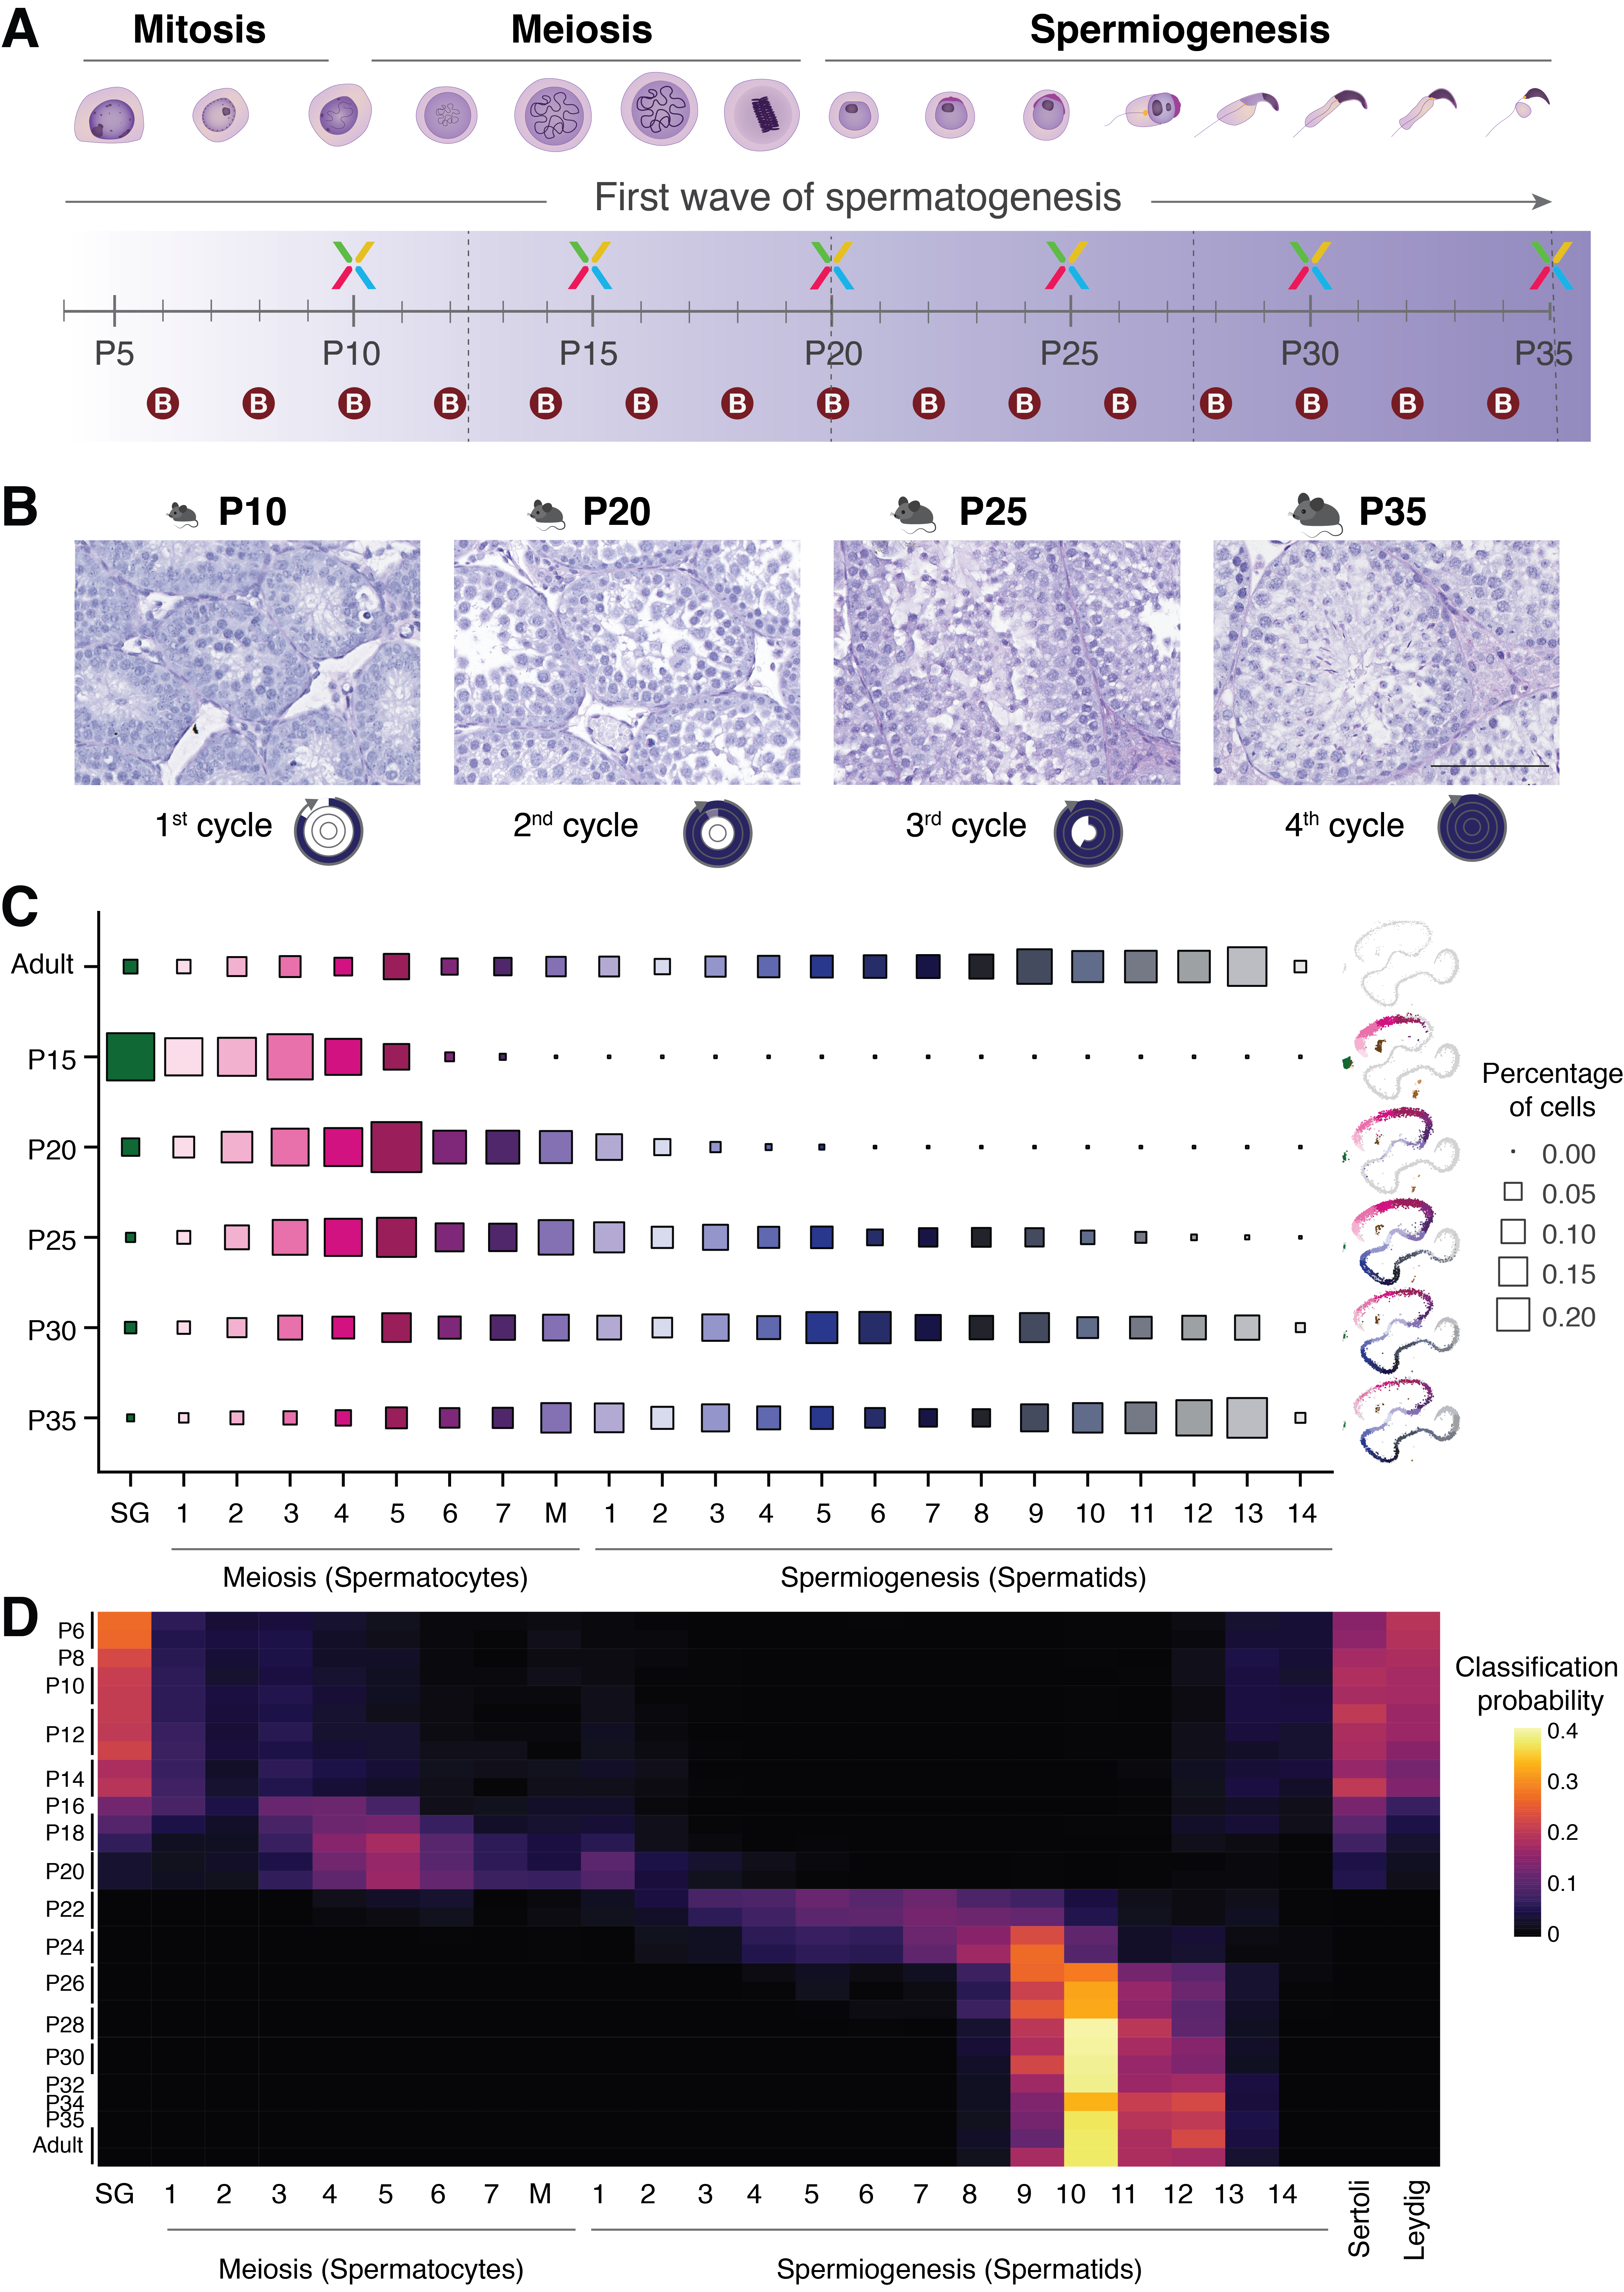
\includegraphics[width=0.95\textwidth]{Fig_4.png}
\caption[Staging of cell types during mouse spermatogenesis]{\textbf{Staging of cell types during mouse spermatogenesis (full legend on next page).}}
\label{fig3:1st_wave}
\end{figure}

\newpage

\captionsetup[figure]{list=no}
\addtocounter{figure}{-1}   
\captionof{figure}{\textbf{Staging of cell types during mouse spermatogenesis (continued).}\\
\textbf{(A)} Schematic representation of the major germ cell types and their corresponding developmental processes. Spermatogonia differentiate undergoing mitotic cell divisions before forming spermatocytes that divide by meiotic division. Following meiosis, spermatids differentiate throughout spermiogenesis to form mature sperm. The timeline in the lower panel indicates at which point during the first wave of spermatogenesis samples were harvested for the generation of scRNA-Seq (X) or bulk RNA-Seq (B) data, \textbf{(B)} Representative images of seminiferous tubules from animals harvested at different postnatal (P) time points during the first wave of spermatogenesis. The approximate timing of the stage and cycle of the tubule is illustrated below in the form of a circle (see \textbf{Fig.~\ref{fig3:cell_staging}B}), \textbf{(C)} After cell mapping and clustering, the percentage of cells in each cluster can be calculated for each sample. The size of squares corresponds to this percentage and the colours indicate the cluster labels depicted in \textbf{Fig.~\ref{fig3:cell_types}C}. tSNEs on the right-hand side of each panel (juvenile samples only) illustrate progress through spermatogenesis. SG: Spermatogonia, M: Metaphase, \textbf{(D)} Probabilistic mapping of bulk RNA-Seq libraries to the cell clusters identified in the adult scRNA-Seq data using a random forest approach. The colour gradient indicates the probability with which a bulk sample can be assigned to the specific cell cluster.  \\}
\captionsetup[figure]{list=yes}

In adults, we detect a homogeneous distribution of cells across the germ cell types ranging from spermatogonia to S14 spermatids \textbf{(Fig.~\ref{fig3:1st_wave}C)}. To characterise germ cell types, we focused on samples taken from P15-P35 animals since at P10, the majority of cell types do not show germ cell properties \textbf{(Fig.~\ref{fig3:cell_types}A)}. In earlier stages, cells are enriched for the most mature cell type in each cycle. For instance, at P15 the majority of cells are spermatogonia and spermatocytes progressing through the mid-pachytene stage \citep{Turner2004}. Interestingly, less mature cell types that exist prior to the mid-pachytene stage are also present at this (and later) time points. This supports recent reports that the first wave of spermatogenesis is less synchronised than previously anticipated \citep{Snyder2010}. At P20, we detect an enrichment for spermatocytes, cells undergoing meiotic cell division, and a small group of early round spermatids. This population structure is in line with matched histology, which shows a large number of tubules in late stages IX-XII and the first occurrence of early round spermatids \citep{Bellve1977}. It has been shown that spermatids first reach the elongating state, which occurs from S10 spermatids onwards, between P24 and P26 \citep{Janca1986}. At P25, we observed that cells mapped to our first ten clusters of spermatids, which we then labelled according to morphologically-defined spermatid substages S1 – S10 \textbf{(Fig.~\ref{fig3:1st_wave}C)}. At P30 and P35, we observed a relatively even distribution of cells across all groups, closely resembling the adult distribution up to S14, indicating that the first wave of spermatogenesis is complete. With this computational mapping of cells collected at different developmental time points, we linked transcriptional profiles of single cells to morphologically defined transitions during germ cell development.

\newpage

\subsection{Classification of cell types based on bulk RNA-Seq data}

While the analysis performed above determines crucial developmental transitions during spermatogenesis, we did not achieve the high-resolution required for the mapping of defined developmental cell types to the clusters identified above. To further validate the identity of the cell clusters, we used bulk RNA-Seq from testis collected during the first wave of spermatogenesis. These samples were harvested every two days between P6 and P34 and allowed us to refine the mapping analysis performed above \textbf{(Fig.~\ref{fig3:1st_wave}A)}. The batch-correction approach used above was developed to match hundreds of single cells across samples and is not suitable to map the 30 bulk RNA-Seq samples onto the adult trajectory. To classify each bulk RNA-Seq sample to one or multiple clusters identified in the scRNA-Seq data, we used a regression approach that performs probabilistic classification. Using the top 50 cluster-specific marker genes for spermatogonia, all spermatocyte groups, all spermatid groups, sertoli and leydig cells, we trained a random forest classifier (implemented in the \emph{randomForest} R package \citep{Liaw2002}) on 2000 cells isolated from adult B6 testes. Model testing was performed on the remaining 1215 cells isolated from adult B6 testes. Prior to training and testing, log$_2$-transformed, normalised counts were scaled by computing the Z score for each gene. Probabilistic prediction was performed using the Z score of log$_2$-transformed, normalised bulk RNA-Seq reads of the input genes. The output of this analysis is the classification probability for each bulk RNA-Seq sample to belong to each scRNA-Seq cluster.\\

This classification confirmed that between P6 – P14 spermatogonia and somatic cells contributed most to the transcriptomic profile \textbf{(Fig.~\ref{fig3:1st_wave}D)}. Between P16 and P20 we observed the emergence of spermatocyte-specific gene expression signatures, after which spermatids become the transcriptionally dominant cell type. By P26, spermatids reach the elongating state where transcription is uniformly shut-down due to the beginning of the histone-to-protamine transition \citep{Steger1999}. Following this, changes in RNA content are mostly due to degradation. Bulk transcriptional profiles can only be classified up to S10 because transcription is largely inactive thereafter and no new cluster-specific marker genes emerge.  

\newpage

\section{Under-represented cell types in spermatogenesis}

The analysis of early stages of juvenile mice in the previous section showed an enrichment for cell types that are relatively under-represented in later stages and in adults (e.g.~spermatogonia and early spermatocytes at P15, \textbf{Fig.~\ref{fig3:1st_wave}C}). Additionally, we detected the absence of germ cells in the P10 sample which leads to a relative enrichment of somatic cell types \textbf{(Fig.~\ref{fig3:cell_types}A)}. This relative enrichment allows us to dissect somatic cell types and spermatogonial differentiation at higher resolution compared to cells isolated from adult samples.

\subsection{Somatic cell types in juvenile testes}

To study heterogeneity within the somatic cell population, we focused on the P10 stage, where somatic cells are relatively more frequent \textbf{(Fig.~\ref{fig3:somatic_cells})}. As expected, we identify substantial numbers of Sertoli and Leydig cells, which are the main somatic cell types in adult. Leydig cells are the primary producers of steroid hormones such as testosterone that regulate sexual differentiation and development of secondary sex characteristics \citep{Svechnikov2010, Haider2004}. Sertoli cells on the other hand reside inside the tubules and provide the structural features required for testis development. They further support differentiating germ cells by providing growth factors and nutrients  \citep{Griswold1998}. In addition, we newly identified a large population of \gls{IL} cells, based on \textit{Dlk1} expression \citep{Lottrup2014}. ILs shape the embryonic development of testes and rapidly decline in numbers after birth \citep{Griswold2009}. \\

Furthermore, we detected the cells that form the basal lamina. These include \gls{PTM} cells (\textit{Acta2}, \citep{Cool2008}), vascular \glspl{EC} (\textit{Tm4sf1}, \citep{Shih2009}), and \glspl{tMg} (\textit{Cd14}, \citep{Kitchens2000}) \textbf{(Fig.~\ref{fig3:somatic_cells}A and B)}. PTM are contractile cells that form the wall of seminiferous tubules and induce the release of the testicular fluid which contains mature spermatozoa \citep{Diez-Torre2011}. In addition, endothelial cells play a major role in forming the testis cord during development and together with PTMs surround Sertoli cells in the adult testes \citep{Combes2009}. Testicular macrophages are the most abundant immune cell type in the organ and play a crucial role in testes development by expressing anti-inflammatory cytokines that induce a tolerogenic environment in testes. This is needed since germ cell specific antigens are only expressed after puberty when the immune system has already matured \citep{Fijak2006}. By performing differential expression analysis (using the \emph{findMarkers} function in \emph{scran}), we identified novel markers for these cell populations that are relatively under-represented in adult testes. \textbf{Fig.~\ref{fig3:somatic_cells}B} visualises the top marker genes for the enriched somatic cell types detected at P10.\\

\begin{figure}[!h]
\centering
\includegraphics[width=\textwidth]{Fig_5.png}
\caption[Enrichment of under-represented somatic cell types in juvenile samples]{\textbf{Enrichment of under-represented somatic cell types in juvenile samples.} \\
\textbf{(A)} tSNE representation of cells isolated from P10 animals that were mapped to cells from adult mice. Cell types were identified by unbiased, graph-based clustering and annotated after marker gene extraction. SG: Spermatogonia, SC: Spermatocytes, IL: Immature Leydig, PTM: Peritubular Myoid Cells, EC: Endothelial Cells, tMg: testicular Macrophages, \textbf{(B)} Heatmap representation of cell type-specific marker genes. Gene in bold are previously described markers of the following cell type: Sertoli cells (\textit{Cst12}), early spermatocytes (\textit{Sycp1}), spermatogonia (\textit{Dmrt1}), immature Leydig cells (\textit{Dlk1}), endothelial cells (\textit{Acta2}), peritubular myoid cells (\textit{Tm4sf1}), Leydig cells (Insl3), testicular macrophages (\textit{Cd14}), \textbf{(C)} PCA of spermatogonia (SG) and early spermatocytes (SC 1) from P10 and P15 animals. 
}
\label{fig3:somatic_cells}
\end{figure}

Furthermore, we detect a relative enrichment of spermatogonia compared to other germ cell types at P10 and P15 \textbf{(Fig.~\ref{fig3:somatic_cells}C)}. Using this large amount of stem cell like cells sampled from different time points during development allows us to dissect its differentiation programme.

\newpage

\subsection{Spermatogonial differentiation}

In the mouse, spermatogenesis is initiated with the division of a type A spermatogonia, also termed A$_{\text{single}}$, to form first a pair, and then a connected chain of undifferentiated spermatogonia (A$_{\text{paired}}$ and A$_{\text{aligned}}$) \citep{Oakberg1971, DeRooij1973}. These cells have competency to undergo spermatogonial differentiation, which involves six transit-amplifying mitotic divisions generating A$_{1-4}$, Intermediate (In), and B spermatogonia, which then give rise to pre-leptotene spermatocytes (Pl) \citep{DeRooij2000} \textbf{(Fig.~\ref{fig3:cell_staging}C)}. Given this, we expect a high level of heterogeneity within the spermatogonia population but identifying spermatogonial sub-populations in adult testes is greatly complicated by their rarity relative to other germ cell types \citep{Lukassen2018}. However, as shown above, during early juvenile development spermatogonia are relatively enriched, which we exploited to further characterise their heterogeneity \textbf{(Fig. \ref{fig3:spermatogonia}A)}. \\

By combining cells from P10 and P15, we obtained 1,186 transcriptional profiles that capture sub-populations during spermatogonial differentiation \textbf{(Fig.~\ref{fig3:spermatogonia}B)}. To jointly analyse transcriptomes of P10 and P15 samples, we performed batch correction between these samples as described above and clustered batch corrected data using a graph-based approach. In order to label the cell types corresponding to the different clusters, we performed marker gene detection using the \emph{findMarker} function in \emph{scran}. By visualising the individual marker genes, we detect two clusters corresponding to undifferentiated spermatogonia (A$_\textnormal{undiff}$) based on their expression of \textit{Nanos3} and \textit{Zbtb16} \textbf{(Fig. \ref{fig3:spermatogonia}B and C)} \citep{Buaas2004, Lolicato2008}). These cells comprise A$_\textnormal{s}$, A$_\textnormal{paired}$, and A$_\textnormal{aligned}$ spermatogonia that decrease in stemness as they divide and gain competency to differentiate \citep{Suzuki2012}. Additionally, these cells express a number of marker genes also detected in undifferentiated human spermatogonial stem cells, such as \textit{Gfra1}, \textit{Bcl6} and \textit{Id4} \citep{Guo2017}. Based on the expression of \gls{Stra8}, we can map the point at which spermatogonial differentiation is induced (A$_\textnormal{aligned}$-to-A$_\textnormal{1}$ transition), thus marking the beginning of differentiating spermatogonia (A$_\textnormal{diff}$) \citep{Endo2015} \textbf{(Fig. \ref{fig3:spermatogonia}B)}. A$_\textnormal{diff}$ are marked by the expression of \textit{Sohlh1} \citep{Ballow2006} and are highly proliferative, generating A$_\textnormal{1-4}$, Intermediate and B spermatogonia. Late differentiating spermatocytes express \textit{Dmrtb1}, which mediates the mitosis-to-meiosis transition and quickly disappears in pre-leptotene spermatocytes \textbf{(Fig. \ref{fig3:spermatogonia}B)}. This latter population shows a second increase in \textit{Stra8} expression levels, which is necessary for initiation of meiosis \textbf{(Fig.~\ref{fig3:spermatogonia}B and C)} \citep{Anderson2008, Endo2015, Zhang2014}. 

\newpage

\begin{figure}[!h]
\centering
\includegraphics[width=0.9\textwidth]{Fig_6.png}
\caption[Cellular heterogeneity during spermatogonial differentiation]{\textbf{Cellular heterogeneity during spermatogonial differentiation.}\\
\textbf{(A)} Schematic representation of spermatogonial differentiation including sub-stages of undifferentiated (A$_\textnormal{s}$, A$_\textnormal{paired}$, A$_\textnormal{aligned}$) and differentiating (A$_\textnormal{1}$, A$_\textnormal{2}$, A$_\textnormal{3}$, A$_\textnormal{4}$, In, B) spermatogonia (SGs) as well as pre-leptotene spermatocytes (Pl), \textbf{(B)} Sub-structure detection in spermatogonia isolated from P10 and P15 animals. PCA was computed on transcriptomes after batch correction between P10 and P15 samples. The first three panels represent expression of known marker genes for undifferentiated (Undiff, \textit{Nanos3}) and differentiating (Diff, \textit{Stra8} and \textit{Dmrtb1}) spermatogonia. The colour scale shows log$_2$-transformed, normalised counts. The last panel overlays cluster identity by sub-clustering batch-corrected transcriptomes of spermatogonia, \textbf{(C)} Z score of normalised expression counts of the top 15 marker genes per cell cluster. Column and row labels represent the cell clusters identified in the last panel of (B). The lower bar indicates the gradual differentiation from undifferentiated spermatogonia to pre-leptotene cells driven by two \gls{RA} signals. }
\label{fig3:spermatogonia}
\end{figure}

\newpage

\subsection{Leptotene and zygotene spermatocytes}

The transition between differentiating spermatogonia and spermatocytes is a gradual process that occurs in stage VIII tubules when B spermatogonia divide and form pre-leptotene spermatocytes \citep{Anderson2008, Baltus2006}. When visualising the first two components of a PCA, we did not observe a continuous differentiation trajectory bridging spermatogonia to spermatocytes \textbf{(Fig.~\ref{fig3:somatic_cells}C)} which indicates a possible loss of cells that characterise the transition between these two cell types. One possible explanation is that leptotene and zygotene spermatocytes have decreased transcriptional activity \citep{Kierszenbaum1974, Monesi1965}, and are thus likely to be classified as empty droplets by the 10X CellRanger pipeline. \\

To capture these transcriptionally quiescent cells, we used the \emph{emptyDrops} function from the \emph{DropletUtils} R package to distinguish between droplets capturing genuine cells with low transcriptional complexity and empty droplets containing only ambient mRNA \citep{Lun2018}. Applying this approach increased the number of early spermatocytes in all samples and, in particular, identified a population of cells connecting spermatogonia and spermatocytes at the predicted position in the cell trajectory \textbf{(Fig.~\ref{fig3:emptyDrops}A-C)}. We strongly enrich for leptotene and zygotene spermatocytes, especially in the P15 sample, after including these smaller cells in the analysis. Due to low transcriptional complexity, these two cell types cluster together which makes it hard to detect a clear mitosis-to-meiosis transition \textbf{(Fig.~\ref{fig3:emptyDrops}B and C)}. As expected for leptotene and zygotene spermatocytes, these cells show high mRNA levels for genes involved in synaptonemal complex formation, chromosome synapsis and DNA double-strand break (DSB) formation such as \textit{Sycp1}, \textit{H2afx} and \textit{Hormad1} \citep{Daniel2011, Mahadevaiah2001, Vries2005} \textbf{(Fig.~\ref{fig3:emptyDrops}D)}.\\

In addition to early spermatocytes, droplets with lower transcriptional complexity also captured late condensing spermatids. As mentioned above, these late stages of spermiogenesis are characterised by continuous degradation of RNA after transcriptional shut-down at the round-to-elongating transition \citep{Steger1999} \textbf{(Fig.~\ref{fig3:emptyDrops}E)}. Nevertheless, including droplets with low transcriptional complexity increases the risk of including low-quality cells and debris. In our case, the large cluster of unidentified cells in \textbf{Fig.~\ref{fig3:emptyDrops}A} could represent membrane vesicles containing RNA at the end of spermiogenesis that form during a process termed "cytoplasmic extrusion" \citep{Rengan2012}.\\

\newpage

\begin{figure}[!h]
\centering
\includegraphics[width=0.75\textwidth]{Fig_7.png}
\caption[Transcriptionally silent cell types in spermatogenesis]{\textbf{Transcriptionally silent cell types in spermatogenesis.} \\
\textbf{(A)} tSNE representation of cells selected by the \emph{emptyDrops} filtering strategy. Coloured dots represent annotated cell types detected using the default \emph{CellRanger} filtering pipeline while black dots represent cells detected by the \emph{emptyDrops} filtering. SG: Spermatogonia, SC: Spermatocytes, IL: Immature Leydig, PTM: Peritubular Myoid Cells, EC: Endothelial Cells, tMg: testicular Macrophages, S: Spermatids, \textbf{(B)} tSNE representation of emptyDrops filtered cells from the P15 sample. Cell colouring corresponds to clustering performed on this sample. Undiff SG: undifferentiated spermatogonia, Diff SG: differentiating spermatogonia, \textbf{(C)} PCA representation of spermatogonia and spermatocytes detected in the P15 sample after \emph{emptyDrops} filtering. Labelling corresponds to the clusters shown in (B), \textbf{(D)} Leptotene and zygotene spermatocyte marker gene expression. The colour scale represents log$_2$-transformed, normalised counts, \textbf{(E)} Visualisation of the number of genes expressed (> 0 counts) per cell.}
\label{fig3:emptyDrops}
\end{figure}

\newpage

\section{Characterisation of male meiosis}

After characterising the major germ and somatic cell types, we next profiled the transcriptional programmes of known developmental processes during spermatogenesis. These include firstly meiosis and later on spermiogenesis which will be analysed and discussed in the next section.\\

The mitotic expansion of spermatogonia produces large numbers of spermatocytes, which then undergo male meiosis where two consecutive cell divisions give rise to four haploid spermatids. In contrast to mitotic cell divisions, prophase of meiosis I is extremely prolonged, lasting up to 10 days in male mice \citep{Soh2017}. Furthermore, meiosis includes programmed DSB formation, homologous recombination, and chromosome synapsis \citep{Marston2004}, which represent molecular processes to induce genetic variation between offspring. Most meiotic processes have been histologically described, but a full transcriptional characterisation of spermatocytes undergoing meiosis is lacking. \\

The continuum of sampled cell types allows us to perform in-depth characterisation of transcriptional changes that occur during meiosis. For this, we ordered spermatocytes along their differentiation trajectory by fitting a principal curve \citep{Hastie1989} to the first 3 principal components using the \emph{principal.curve} function implemented in the \emph{princurve} R package. This approach allows us to order cells along the developmental trajectory. The directionality of the trajectory was inferred using prior information based on the cluster annotation. Here, the ordering of cell types is as follows: leptotene spermatocytes (SCs, not present in CellRanger filtered data), zygotene SCs, pachytene SCs, diplotene SCs and finally cells in metaphase \textbf{(Fig.~\ref{fig3:meiosis}A)}. \\

To detect molecular processes that occur during meiosis, we first profiled the overall transcriptional rate before dissecting changes in expression on a gene-specific level. As shown before \citep{Xia2018}, we identified a strong increase in the number of genes expressed as spermatocytes progress through prophase, with the highest number being expressed immediately before the cells divide \textbf{(Fig.~\ref{fig3:meiosis}A)}. Using this as a proxy for active transcription, we identified diplotene spermatocytes, which are the latest cell type in prophase I in which RNA synthesis is occurring \citep{Monesi1965}. 

\newpage

We used the increase and later decrease in transcription as a guide for the progressive changes in transcription throughout meiosis. Therefore, to detect functional genes that influence this process, we correlated each gene’s normalised expression level to the number of genes expressed. For this, we used the \emph{correlatedPairs} function implemented in \emph{scran} \citep{Lun2016}. First, we constructed an empirical null distribution using the \emph{correlateNull} function implemented in \emph{scran}. Next, we tested the observed Spearman’s $\rho$ for each gene against this null distribution. Genes with $\rho$ < -0.3 and a Benjamini-Hochberg corrected empirical p-value < 0.1 were considered as negatively correlated and genes with $\rho$ > 0.3 and a Benjamini-Hochberg corrected empirical p-value < 0.1 were considered as positively correlated.\\

As expected, previously known marker genes for early meiotic processes such as \textit{Hormad1} and \textit{Sycp3} decreased in expression during Prophase I, whereas \textit{Pou5f2} and \textit{Tcte2}, a male meiosis-specific gene \citep{Braidotti1997} increased in expression \textbf{(Fig.~\ref{fig3:meiosis}B)}. Supporting our identification of diplotene spermatocytes, \textit{Pou5f2} has previously been shown to be specifically expressed during a 36- to 48-hour period preceding the meiotic cell division \citep{Andersen1993}. \\

In the next step, we performed a targeted analysis and detected marker genes for each of the spermatocyte sub-cell types. Despite the overall increase in transcription, we observed distinct temporal expression patterns when visualising these specific marker genes for individual spermatocyte populations. Even within pachytene spermatocytes at different stages in their developmental progression, there exists substantial heterogeneity \textbf{(Fig.~\ref{fig3:meiosis}C)}. As expected, early spermatocyte markers (SC 1 and SC 2) were enriched for genes with known functions in male or female fertility such as \textit{Piwil1} (\textit{Miwi}), \textit{Cks2}, \textit{Sycp1}, reflecting a history of intensive investigation \citep{Deng2002, Spruck2003, Vries2005}. We performed literature search and used the database \url{www.mousephenotype.org} to annotate genes regarding their sterility phenotype. \\

In sum, we dissected the transcriptional heterogeneity within spermatocytes undergoing meiosis and identified a set of genes that form potential drivers for this process. Genes which show a high expression in early stages during meiosis have been validated to induce sterility once removed from the system.  

\newpage

\begin{figure}[!h]
\centering
\includegraphics[width=0.9\textwidth]{Fig_8.png}
\caption[Gene expression dynamics during male meiosis]{\textbf{Gene expression dynamics during male meiosis.} \\
\textbf{(A)} Number of genes expressed per spermatocyte. Cells are ordered by their developmental progression during meiotic prophase until metaphase, \textbf{(B)} Expression of genes that are negatively or positively correlated with the number of genes expressed during meiotic prophase (negatively correlated: $\rho$ < -0.3, Benjamini-Hochberg corrected empirical p-value < 0.1; positively correlated: $\rho$ > 0.3, Benjamini-Hochberg corrected empirical p-value < 0.1). Per category, two genes are visualised. The colour gradient represents log$_2$-transformed, normalised counts, \textbf{(C)} Heatmap visualising the Z score scaled expression of the top 15 marker genes per cell type. Row and column labels correspond to the different populations of spermatocytes (SC). M: Metaphase. Genes are labelled based on their fertility phenotype: pink – infertile or sub-fertile in females, light blue - infertile or sub-fertile in males, dark green - infertile or sub-fertile in both males and females. The sterility phenotype was annotated using \url{www.mousephenotype.org.}}
\label{fig3:meiosis}
\end{figure}

\section{Transcriptional dynamics during spermiogenesis}
\label{sec3:spermiogenesis}

Once the meiotic divisions result in the production of four haploid cells, round spermatids progress to form first elongating and finally mature sperm during a process termed "spermiogenesis" \textbf{(Fig.~\ref{fig3:spermiogenesis}A)}. A key event during spermiogenesis is chromatin condensation, which is required to package the haploid genome into the confined space of the sperm nucleus. Our data allowed us to dissect at high-resolution the transcriptional regulation needed for gradual chromatin remodelling during spermatid differentiation, involving the replacement of canonical histones by histone variants followed by transition proteins and eventually protamines \citep{Balhorn2007, Kennani2017}. This chromatin remodelling later induces a transcriptional shut-down where changes in RNA content are purely driven by degradation \citep{Steger1999}.

\subsection{Expression of chromatin components during spermiogenesis}

We first explored how expression of histone variants changed throughout early spermatid maturation \textbf{(Fig.~\ref{fig3:spermiogenesis}A)}. Similar to the developmental ordering presented in the previous section, we ordered cells by fitting a principal curve to the first three principal components calculated on S1-S14 spermatids. Annotations for histone variants and canonical histones were taken from El Kennani \emph{et al.}, 2017 \citep{Kennani2017}. Multiple variants of H3 and H2A are expressed in spermatocytes \citep{Greaves2006, Mahadevaiah2001, Tang2015}, and our data showed that many of these histones are highly expressed in early round spermatids. For instance, Histone H3.3 is a histone variant consisting of two genomic copies (\textit{H3f3a} and \textit{H3f3b}). Across spermatogenesis, we observed distinct expression patterns for the two genes, with \textit{H3f3a} being consistently highly expressed until the transcriptional shut-down at spermatid stage S10. In contrast, \textit{H3f3b} showed a much more dynamic expression profile, starting at a high level in spermatocytes, dropping throughout meiotic prophase, followed by up-regulation in round spermatids \textbf{(Fig.~\ref{fig3:spermiogenesis}B)}. Although both genes have been implicated in male fertility, the phenotypes associated with perturbations of the more dynamically regulated paralog \textit{H3f3b} are much more severe \citep{Tang2015, Yuen2014}.\\

When profiling the expression of canonical histones, we detected increased expression of \textit{Hist1h2bp} and \textit{Hist1h4a}, with a distinct up-regulation during early and mid-spermiogenesis \textbf{(Fig.~\ref{fig3:spermiogenesis}C)}. Canonical histones are typically transcribed in a replication-dependent manner during S phase \citep{Marzluff2002}, thus the atypical expression during spermiogenesis could suggest important roles as replacement histones during chromatin remodelling. Nevertheless, canonical histones appeared to be the set of annotated histones that is least correlated to the developmental trajectory \textbf{(Fig.~\ref{fig3:spermiogenesis}A)}.

\begin{figure}[!h]
\centering
\includegraphics[width=0.85\textwidth]{Fig_9.png}
\caption[Transcriptional dynamics and chromatin remodelling during spermiogenesis]{\textbf{Transcriptional dynamics and chromatin remodelling during spermiogenesis.} \\
\textbf{(A)} Z score scaled, normalised expression of histone variants (H1, H2A, H2B, H3), canonical histones, \glspl{Tnp} and \glspl{Prm} during spermiogenesis. Cells were ordered based on their developmental trajectory ranging from round spermatids (S1-S8) to elongating spermatids (S9-S14), \textbf{(B)} Expression of \textit{H3f3a} (middle panel) and \textit{H3f3b} (right panel) across the different germ cell populations, \textbf{(C)} Similar visualisation as in (B) for \textit{Hist1h4a} expression across germ cells. }
\label{fig3:spermiogenesis}
\end{figure}

\newpage

We next profiled the transcriptional dynamics of testis-specific histone variants. They showed highest expression in elongating spermatids, with most variants increasing strongly in expression from S5 onwards. While some variants had a consistently high expression level, \textit{Hils1} and \textit{H1fnt} decreased in expression towards the late stages, similarly to \textit{Tnp1} and \textit{Tnp2} \citep{Zhao2004}. Both histone variants are important for male fertility, and \textit{Hils1} has previously been shown to interact with \textit{Tnp1} \citep{Tanaka2005}. In contrast, three testis-specific histone variants \textit{Hypm}, \textit{H2afb1} and \textit{H2bl1} (\textit{1700024p04rik}) showed consistently high expression until the end of differentiation similar to protamines, suggesting these variants may contribute to the final genome condensation.

\subsection{Identifying the point of transcriptional shut-down}

As a consequence of chromatin condensation, transcription ceases in spermatids at the round to elongating switch, consistent with the lack of active RNA Pol II at S10 and later stages \citep{DottermuschHeidel2014}.
By fitting a smooth regression (loess) to the number of genes expressed per cell along the differentiation trajectory, we easily identified the point of transcriptional shut-down. The number of expressed genes is stable until approximately S9 before gradually declining by roughly 50\% \textbf{(Fig.~\ref{fig3:transcriptional_shutdown}A)}. In the 8 days following transcriptional shut-down, spermatids still need to undergo drastic morphological changes, including the assembly of sperm-specific structures such as the flagellum, before mature testicular sperm can be released into the lumen \citep{ODonnell2014}. To achieve this in the absence of active transcription, spermatids store large amounts of mRNAs in a perinuclear RNA granule termed the chromatoid body \citep{Kotaja2007}. RNA stored in the chromatoid body is then released for translation, suggesting that these molecules may play vital roles during late stages of spermiogenesis. However, identifying the RNAs that are stored has been hindered by difficulties in purifying late spermatids. \\

By correlating normalised gene expression against the number of genes expressed, we identified a large number of genes that gradually decrease in relative expression after transcriptional shut-down. We reasoned that transcripts where the relative expression after transcriptional shut-down appeared to increase are likely protected from degradation \textbf{(Fig. \ref{fig3:transcriptional_shutdown}B)}. This included genes with well-known spermiogenesis-specific functions. Among those that relatively increase in expression, we find transition proteins and protamines that are involved in chromatin condensation. Furthermore, we detect genes that are involved in the development of sperm motility such as \gls{Akap4} and \gls{Cabs1} \citep{Kawashima2009, Miki2002}. 

\newpage

\begin{figure}[!h]
\centering
\includegraphics[width=\textwidth]{Fig_10.png}
\caption[Transcriptional shut-down during spermiogenesis]{\textbf{Transcriptional shut-down during spermiogenesis.} \\
\textbf{(A)} Number of genes expressed per spermatid. Cells were ordered based on their developmental trajectory. Red line indicates a smooth regression (loess) fit, \textbf{(B)} For each gene, its normalised expression per cell was correlated with the number of genes expressed per cell. Genes were ordered based on the correlation coefficient and grouped into 9 sets. Z score scaled expression was averaged across genes within each gene set. Vertical dashed line indicates transcriptional shut-down between S9 and S10.}
\label{fig3:transcriptional_shutdown}
\end{figure}

With this analysis, we explored transcriptional processes occurring throughout the process of spermiogenesis that (i) regulate the expression of chromatin components and (ii) lead to the degradation of unneeded transcripts.

\newpage

\section{Meiotic silencing dynamics of sex chromosomes}

A male-specific feature of meiosis is the transcriptional silencing of sex chromosomes, followed by a partial reactivation in post-meiotic spermatids. This process is termed \gls{MSCI}, and is caused by asynapsis of the sex chromosomes, leading to accumulation of phosphorylated \gls{H2afx} and the formation of the sex body \citep{Hamer2003} \textbf{(Fig.~\ref{fig3:X_reactivation}A)}. We next profiled transcriptional changes mediated by the inactivation and reactivation of the sex chromosomes in single-cell and bulk RNA-Seq data. \\

To assess overall transcriptional dynamics of the sex chromosomes, we computed the ratio of expression from the X and Y chromosome and chromosome 9 to all autosomes. For this, we selected genes that were expressed in more than 30\% of spermatogonia or 30\% of spermatids, the cell types with detectable sex chromosome expression. For each cell, the mean expression across these genes per chromosome was calculated. Mean expression of the sex chromosomes and chromosome 9 was divided by mean expression across all autosomes. By plotting the ratio of gene expression from the X or Y chromosomes compared to all autosomes, the inactivation and re-activation status of the sex chromosomes can be inferred \textbf{(Fig.~\ref{fig3:X_reactivation}B)}. \\

The X chromosome is partially up-regulated in spermatogonia as described by Sangrithi \emph{et al.}, 2017 (\gls{XA} ratio < 1) \citep{Sangrithi2017}. This is followed by transcriptional silencing in spermatocytes. Throughout spermiogenesis, expression from the X chromosome gradually increases, reaching X:A ratios comparable to spermatogonia, therefore suggesting a substantial reactivation of the X chromosome in post-meiotic spermatids. We detect similar behaviour for the Y chromosome but due to the small number of expressed genes, the signal is noisier \textbf{(Fig.~\ref{fig3:X_reactivation}B)}. In comparison, chromosome 9 shows consistent expression across all cell types throughout spermatogenesis (9:A $\approx$ 1).\\

Transcriptional silencing was originally thought to persist throughout post-meiotic development \citep{Greaves2006, Turner2006}. However, several genes have been shown to be re- or \emph{de novo} activated in spermatids, some of which are dependent on \gls{Rnf8} and/or \gls{Scml2} \citep{Hasegawa2015a, Sin2012, Sin2015}. The precise timing and order of the transcriptional reactivation of \emph{de novo} escape genes during spermiogenesis has not been explored. We therefore first classified \emph{de novo} activated escape genes using bulk RNA-Seq data and profiled their temporal expression directly following meiosis.\\

Profiling whole-testis transcriptomes of juvenile mice sampled every two days during the first wave of spermatogenesis allowed the sensitive detection of spermatid-specific escape genes \textbf{(Fig.~\ref{fig3:cell_staging}A)}. Due to the gradual emergence of germ cell types during the first spermatogenic wave, differential expression analysis between early ($\leq$ P20) and late (> P20) time points revealed genes exclusively expressed in spermatids and which are thus \emph{de novo} activated escape genes (n = 128) \textbf{(Fig.~\ref{fig3:X_reactivation}C)}. We used \emph{edgeR} to identify differentially expressed genes between these conditions \citep{Robinson2009}. Spermatid-specific genes are identified with a log$_2$-fold change > 5 in samples after day 20 compared to samples before day 20 (controlling the FDR to 10\%). \\

Within the set of \emph{de novo} activated escape genes we find many of the previously annotated escape genes such as \textit{Cypt1}, \textit{Cycl1}, and \textit{Akap4}. Interestingly, this set of genes show an enrichment for targets of H3K27 acetylation which is mediated by \textit{Rnf8} or \textit{Scml2} (Fisher's Exact Test: \textit{Rnf8}-targets, p-value < 5x10$^{-12}$; \textit{Scml2}-targets, p-value < 2x10$^{-9}$) \textbf{(Fig. \ref{fig3:X_reactivation}C)}. This chromatin mark represents active enhancers necessary for the reactivation of gene expression in spermatids \citep{Adams2018}. \\

While the bulk RNA-Seq data is ideal for identifying spermatid-specific, \emph{de novo} activated genes, it lacks the temporal resolution to differentiate between early and late reactivated genes. We therefore ordered the 128 \emph{de novo} activated genes based on their peak in expression using the scRNA-Seq data \textbf{(Fig. \ref{fig3:X_reactivation}D)}. The \emph{de novo} activated genes across our single cell RNA-Seq dataset showed a broad range of temporal expression patterns. The earliest expression, directly following meiosis and lasting until stages S4-S5 was observed for three members of the \gls{Ssxb} multi-copy gene family (\textit{Ssxb1}, \textit{Ssxb2}, \textit{Ssxb3}). Multi-copy genes have previously been described to have spermatid-specific expression \citep{Mueller2008}, and their ampliconic structure has been speculated to play a role in escaping meiotic silencing via self-pairing \citep{Disteche2008}.

\newpage

\begin{figure}[!h]
\centering
\includegraphics[width=\textwidth]{Fig_11.png}
\caption[X chromosome dynamics during spermatogenesis]{\textbf{X chromosome dynamics during spermatogenesis.} \\
\textbf{(A)} Schematic of sex chromosome sub-nuclear localisation through spermatogenesis, \textbf{(B)} For each cell, the ratio of mean expression of genes on Chr 9, Chr X and Chr Y to the mean expression of genes across all autosomes is represented as a boxplot for cells allocated to each developmental stage. SG: Spermatogonia, M: Metaphase, \textbf{(C)} Expression of all X chromosome genes (> 10 average counts) in bulk RNA-Seq data across the juvenile time course. Columns correspond to developmental stage and rows are ordered by the log$_2$ fold change between spermatocytes (stages before and including postnatal day (P) 20) and spermatids (stages after P20). Horizontal dashes indicate genes that are targets of \textit{Rnf8} (green) and \textit{Scml2} (blue) \citep{Adams2018}, \textbf{(D)} Average expression of spermatid-specific genes (panel (C)) per germ cell type. Columns are ordered by developmental stage and rows are ordered by peak gene expression through development. Multi-copy genes are highlighted in bold.}
\label{fig3:X_reactivation}
\end{figure}

\newpage

\section{Epigenetic mechanisms of X chromosome reactivation}

After identifying \emph{de novo} activated escape genes, we next profiled the epigenetic basis that might underpin such transcriptional dynamics. For this, we profiled the chromatin landscape in spermatocytes and spermatids using the newly developed CUT\&{}RUN protocol for low cell numbers \textbf{(Appendix \ref{appA.2})} \citep{Skene2018}. 

\subsection{CUT\&{}RUN to profile H3K4me3 and H3K9me3 marks}

In brief, from two individuals, we sorted spermatocytes and spermatids at P26 during the first wave of spermatogenesis \textbf{(Fig.~\ref{fig3:K9_global}A)}. At this stage, tubules contain spermatocytes close to the meiotic cell divisions and elongating spermatids. We assayed H3K4me3 as a proxy for promoter activity, as well as repressive H3K9me3 mark. By profiling the enrichment of H3K9me3 across all chromosomes, we confirmed that the X chromosome has high levels of H3K9me3 in spermatids which has been previously shown \citep{Moretti2016, Greaves2006, Tachibana2007}. In addition, we now show that H3K9me3 accumulation begins earlier in meiosis, and indeed spermatocytes show enrichment of this repressive mark on the X chromosome \textbf{(Fig.~\ref{fig3:K9_global}B)}. \\

On autosomes, H3K9me3 is enriched in pericentromeric regions of constitutive heterochromatin \citep{Peters2001}. To assay the distribution of read pairs across whole chromosomes, we binned reads in 1kb windows across the chromosome. Next, we calculated the cumulative sum across 10,000 randomly sampled bins starting at windows with the highest H3K9me3 enrichment. This measure indicates whether each window contains equal enrichment (slope is similar across the curve) or if some windows are enriched for the mark (slope decreases across the curve). As seen in \textbf{Fig.~\ref{fig3:K9_global}D}, the H3K9me3 enrichment appears to be homogeneously distributed across the X chromosome while, for example, the enrichment of the H3K9me3 mark on chromosome 9 is a lot more heterogeneous. \\

Nevertheless, when merging the 1000 windows with highest H3K9me3 enrichment, we detected broad regions showing particularly high levels of H3K9me3 scattered across the X chromosome \textbf{(Fig.~\ref{fig3:K9_global}C)}. Among the merged regions with highest H3K9me3 enrichment, we detect the promoter of \textit{Akap4}, a well-known escape gene. This discovery prompted us to profile the chromatin dynamics of active and repressive marks at promoters of \emph{de novo} escape genes (\emph{spermatid-specific genes}) versus the promoters of all other expressed X-chromosome genes (\emph{non-spermatid specific genes}) \textbf{(Fig.~\ref{fig3:X_reactivation}C)}.

\begin{figure}[!h]
\centering
\includegraphics[width=\textwidth]{Fig_12.png}
\caption[Chromatin profiling in spermatocytes and spermatids]{\textbf{Chromatin profiling in spermatocytes and spermatids.} \\
\textbf{(A)} Spermatocytes and spermatids were isolated from the same individual using FACS and profiled using H3K4me3 (active mark) and H3K9me3 (repressive mark) using CUT\&{}RUN, \textbf{(B)} Number of H3K9me3 Fragments Per Kilobase per Million (FPKM) for each chromosome. Pink: spermatocytes, blue: spermatids. Shape corresponds to biological replicate, \textbf{(C)} The top 1000 windows with highest H3K9me3 signal (1000 bp width, CPM) were merged using a tolerance of 1500 bp. Representative tracks of one replicate in spermatocytes and one replicate in spermatids are shown, \textbf{(D)} Cumulative summed counts per million across 10000 randomly sampled windows (1000 bp width) visualising the distribution of the H3K9me3 signal across chromosome 9 (dashed line) and chromosome X (solid line).}
\label{fig3:K9_global}
\end{figure}

\newpage

\subsection{Targeted silencing of spermatid-specific escape genes}

Here, we profiled the enrichment for H3K4me3 and H3K9me3 marks at promoters of spermatid-specific escape genes and all other X-linked genes in spermatids and spermatocytes. As a measure for enrichment, we calculated the \gls{CPM} for paired reads per promoter. In spermatocytes, spermatid-specific genes showed lower enrichment in H3K4me3 than non-spermatid specific genes (Wilcoxon-Mann-Whitney: p-value < 2.2x10$^{-16}$) \textbf{(Fig.~\ref{fig3:K9_K4_targeted}A, left panel)}. In contrast, spermatid-specific genes have on average elevated H3K4me3 in spermatids, as expected based on their increased expression level compared to spermatocytes \textbf{(Fig.~\ref{fig3:K9_K4_targeted}A, right panel)}. \\


When examining the deposition of H3K9me3 on the promoters of X-linked genes, we detected a strong enrichment in spermatid-specific escape genes in spermatocytes (Wilcoxon-Mann-Whitney: p-value < 3.7x10$^{-11}$) \textbf{(Fig.~\ref{fig3:K9_K4_targeted}B, left panel)}. This pattern indicates that spermatid-specific genes are more strongly repressed in spermatocytes. Due to the strong enrichment of H3K9me3 on the post-meiotic X chromosome, we detect similar H3K9me3 enrichment in promoters for both spermatid-specific and non-specific X-linked genes \textbf{(Fig.~\ref{fig3:K9_K4_targeted}B, right panel)}.\\

Our results describe the precise epigenetic changes associated with escape gene activation in post-meiotic cells. These dynamics are exemplified by the chromatin remodelling that occurs around \textit{Akap4} and \gls{Cypt1}, both of which are well-studied spermatid-specific genes \textbf{(Fig.~\ref{fig3:K9_K4_targeted}C)}. The promoters of these genes have high levels of H3K9me3 in spermatocytes, which decreases in spermatids, while H3K4me3 levels are strongly increased. This targeted repression of a subset of X-linked escape genes could indicate a mechanism to repress otherwise lethal genes in spermatocytes that are later on needed in spermatid development. Examples of spermatocyte-lethal genes involved in spermatid development are two Y chromosome encoded genes: \gls{Zfy} 1 and 2 \citep{Royo2010}.

\newpage

\begin{figure}[!h]
\centering
\includegraphics[width=\textwidth]{Fig_13.png}
\caption[Targeted repression of spermatid-specifc escape genes in spermatocytes]{\textbf{Targeted repression of spermatid-specifc escape genes in spermatocytes.} \\
\textbf{(A)} and \textbf{(B)} Boxplot of H3K4me3 (A) and H3K9me3 (B) Counts Per Million (CPM) in promoter regions of spermatid specific (n=127) and non-spermatid specific (n=617) genes for spermatocytes (left) and spermatids (right).  \# indicates statistical significance (Wilcoxon-Mann-Whitney: p-value < 1x10$^{-10}$), n.s. – not significant, 
\textbf{(C)} Genome tracks of H3K4me3 and H3K9me3 for two representative spermatid-specific genes (\textit{Akap4} and \textit{Cypt1}) for spermatocytes (left) and spermatids (right). Reads were scaled by library size. The genomic location of these genes is indicated below the tracks where exons are labelled as blocks and the directionality of transcription is shown by arrows.}
\label{fig3:K9_K4_targeted}
\end{figure}

\newpage

\section{Measuring changes in variability over pseudo-time}
\label{sec3:variability_over_PT}

As described above, spermatogenesis is a unidirectional and continuous differentiation process coupled to a complex system of developmental steps. I next asked whether this differentiation process is coupled to changes in transcriptional variability. In mouse haematopoietic cell differentiation, cell-to-cell diversity increases at critical state transitions where cell fate decisions are made \citep{Mojtahedi2016}. A similar effect was detected in chicken erythroid progenitor cells where the Shannon entropy is highest directly at the point of fate commitment and declines upon the irreversible commitment to differentiation \cite{Richard2016}. In the previous chapter, we have demonstrated that transcriptional variability shows dynamic changes during CD4\plus{} T cell differentiation with high variability being observed at a possible early commitment point and a decrease in variability upon proliferation. In this section, I applied the regression BASiCS model, which was developed in the previous chapter, to study changes in transcriptional variability over the time-course of spermatogenesis. More specifically, I profiled changes in variability for individual genes during spermiogenesis, the differentiation process that directly follows meiosis (see \textbf{Section \ref{sec3:spermiogenesis}}). As described above, spermiogenesis is a differentiation process that involves an extensive remodelling of the chromatin with transcriptional shut-down occurring at around spermatid stage S10. Modelling changes in expression over a differentiation time-course is done by ordering transcriptional profiles of individual cells along their so called \emph{pseudo-time}. Different methods have been proposed to perform this ordering based on minimum spanning trees \citep{Trapnell2014} and nearest-neighbour graphs \cite{Setty2016}, Gaussian Processes \citep{Reid2016a, Campbell2016b} and diffusion maps \citep{Haghverdi2016}. Once the pseudo-temporal ordering is determined, genes that change in expression over pseudo-time can be found by fitting a generalised linear model to the expression counts and performing a likelihood ratio test against a null model with no pseudo-time dependence \citep{Trapnell2014}. Profiling changes in variability is more complicated as single-cell measures of variability are not available. 

\subsection{Using BASiCS on continuous data}

Here, I use BASiCS to estimate residual over-dispersion parameters for homogeneous cell populations along the differentiation time-course. Different approaches of identifying homogeneous populations exist. First, ordered cells can be split into populations of equal size (e.g.~200 cells per group). This approach produces heterogeneous cell populations when cell state transitions occur within the population. I therefore rely on the clustering performed in \textbf{Section \ref{sec3:clustering}} which splits the full cell population along the differentiation trajectory. For each cluster from S1 to S14, the regression BASiCS model was run for 40,000 iterations with 20,000 iterations of burn-in and a thinning value of 20. \\

For each gene in each of the 14 spermatid populations, BASiCS generates a posterior distribution estimating the residual over-dispersion parameter in form of an MCMC chain \textbf{(Fig.~\ref{fig3:variability_schematic}A)}. These measures are independent of mean expression (see previous chapter) and can therefore be used to study changes in variability which are not confounded by changes in mean expression throughout the differentiation of sperm. I chose two approaches to profile and test temporal changes of transcriptional variability during spermiogenesis. \\

First, I used the iterative fitting of a linear regression model between the residual over-dispersion parameters and the progression of spermiogenesis to find linear changes in variability. For this, I selected spermatids from stages S1 to S9 prior to transcriptional shut-down. Transcriptional changes after S10 are only due to degradation of mRNA and I assume that linear changes in variability occur before S10. In more detail, for each MCMC iteration, I fit a linear regression model between the current samples of $\epsilon_i$ against the cluster label \textbf{(Fig.~\ref{fig3:variability_schematic}B)}. This fitting is performed for each gene individually and generates a \emph{post hoc} distribution of the intercept and the slope regression coefficient that captures uncertainty in the regression fit. Focusing on the slope coefficient, I can compute the posterior tail probability of the slope coefficient being different from 0. If the posterior tail probability is larger than a threshold (e.g.~80\%), I consider the transcriptional variability of this gene to be either positively or negatively associated with temporal ordering depending on the sign of the median slope coefficient \textbf{(Fig.~\ref{fig3:variability_schematic}B)}. Similar to differential testing described in the previous chapter, the probability threshold is determined by fixing the expected false discovery rate to 10\%. A similar testing can be done for the slope coefficient when fitting a linear model between the group wise mean expression parameter $\log(\mu_i)$ and the group labels.\\

Secondly, to detect non-linear patterns of changes in transcriptional variability, I perform clustering on the gene-specific variability profiles across spermatid populations S1-S14. Similar approaches have been used to find patterns of genes expression across pseudo-time. Common patterns for changes in expression levels include immediate, transient and gradual up- or down-regulation \citep{Trapnell2014}. When profiling changes in variability over the time-course of differentiation these clustered profiles can indicate similarly strong or weak transcriptional regulation or similar expression rates \textbf{(Fig.~\ref{fig3:variability_schematic}C)}.

\newpage

\begin{figure}[!h]
\centering
\includegraphics[width=0.8\textwidth]{Fig_14.png}
\caption[Detecting changes in variability over pseudo-time]{\textbf{Detecting changes in variability over pseudo-time.}\\
\textbf{(A)} For each group of spermatids, BASiCS  generates a posterior distribution of residual over-dispersion parameters $\epsilon_i$. Cell groups can be ordered based on their pseudo-time (upper panel). Lower panels indicate the MCMC chain for gene-specific $\epsilon_i$ per group (A, B, ..., X), \textbf{(B)} For each iteration of the MCMC (1,...,n), a linear regression was fit between the current samples of $\epsilon_i$ against the group labels for spermatids (S) 1-9. This approach generates a \emph{post hoc} distribution of the slope coefficient $\beta_1$ (lower panels). The distribution is used to calculate the posterior probability of observing $\beta_1\neq0$, \textbf{(C)} Clustering was performed on variability profiles across spermatid populations S1 to S14. A smooth regression (loess) was fit to the median $\epsilon_i$'s of the genes within each cluster. Genes that quickly decrease in variability (left panel), increase then decrease in variability (middle panel) or quickly increase in variability (right panel) can be identified.}
\label{fig3:variability_schematic}
\end{figure}

\newpage

\subsection{Finding continuous changes in variability by linear model fitting}

To detect single genes that continuously increase or decrease in variability, I fit a linear regression model to each iteration of the MCMCs sampling $\epsilon_i$ or $\mu_i$ \emph{versus} the group labels \textbf{(Fig.~\ref{fig3:variability_schematic}B)}. The posterior distributions of the slope coefficient were used to categorise genes based on their transcription dynamics along the differentiation time-course (middle panel in \textbf{Fig.~\ref{fig3:linear_variability}}). These categories include: 

\begin{itemize}
\itemsep0em 
\item Increase in mean expression, no change in variability
\item Increase in mean expression, increase in variability
\item Increase in mean expression, decrease in variability
\item Decrease in mean expression, no change in variability
\item Decrease in mean expression, increase in variability
\item Decrease in mean expression, decrease in variability
\item No change in mean expression, no change in variability
\item No change in mean expression, increase in variability
\item No change in mean expression, decrease in variability
\end{itemize}

This approach leads to the detection of few genes that significantly change in variability over the differentiation time-course in a linear fashion while the majority of genes change only in mean expression. One hypothesis is that sperm maturation is a tightly regulated progress where the majority of genes follow a clear transcriptional pattern. Such a process contrasts with other differentiation programmes such as haematopoiesis where branching events occur and the whole cell population expands in transcriptional variability to find new attractor states \citep{Mojtahedi2016}. To visualise changes in transcriptional variability, I selected representative genes from four categories: (i) Increase in mean expression, increase in variability, (ii) Increase in mean expression, decrease in variability, (iii) Decrease in mean expression, increase in variability, (iv) Decrease in mean expression, decrease in variability (see insets in \textbf{Fig.~\ref{fig3:linear_variability}}). Interestingly, \gls{Tsga8}, one of the most rapidly evolving X-linked genes, shows a strong increase in expression and a clear decrease in transcriptional variability. \emph{Tsga8} has been reported to be involved in hybrid sterility where F$_1$ crosses of mice form different strains are unable to reproduce. This effect might be due to the strong divergence of the \emph{Tsga8} sequence between species \citep{Good2011}. A tight regulation of its expression during spermiogenesis can therefore further control the phenotypic effect in F$_1$ animals.

\newpage

\begin{figure}[!h]
\centering
\includegraphics[width=0.8\textwidth]{Fig_15.png}
\caption[Linear changes in variability over spermiogenesis]{\textbf{Linear changes in variability over spermiogenesis.}\\
Linear models were fit between the residual over-dispersion parameter $\epsilon_i$ or the mean expression parameter $\mu_i$ and the groups labels (S) 1-9 for each iteration of the MCMC. Median posterior estimates of the slope parameter of the variability fit were plotted against the slope parameter of the mean expression fit. Each dot represents a single gene. Genes are coloured based on their regulation (legend). Plot insets indicated the Z score scaled normalised expression (upper panel) and the median group-wise residual over-dispersion estimates $\epsilon_i$ (lower panels) of representative genes for four categories.}
\label{fig3:linear_variability}
\end{figure}

\newpage

\subsection{Clustering of variability profiles}

To identify non-linear patterns across all genes, I first ordered variability profiles based on their peak variability \textbf{(Fig.~\ref{fig3:variability_clustering}A)}. Here, variability profiles are represented by the median residual over-dispersion parameter $\epsilon_i$  ordered from S1 to S14. Most variability profiles showed highest variability in one group, albeit other patterns of variability are also detectable. \\

To identify the major patterns of variability across the full range of spermiogenesis, I performed k-means clustering across all variability profiles. In this case, it was required to select the expected number of clusters. Due to the fact that most genes showed peak variability in exactly one group, I selected $\text{k}=20$ to detect patterns other than peaks in single groups. After clustering, I detect a variety of variability patterns ranging from high variability in early spermiogenesis to high variability at later stages \textbf{(Fig.~\ref{fig3:variability_clustering}B)}. Interestingly, I observed patterns that show gradual increase in variability until around spermatid stage S9 and decrease afterwards \textbf{(Fig.~\ref{fig3:variability_clustering}B, middle panel)}. \\

The group with peak variability at around S9 consists of all transition proteins (\textit{Tnp1}, \textit{Tnp2}) and protamins (\textit{Prm1}, \textit{Prm2}, \textit{Prm3}). When visualising the expression patterns of \textit{Prm1}, I detect a rapid shift in expression for cells from S9 \textbf{(Fig.~\ref{fig3:variability_clustering}C, middle panel)}. Similarly, genes that show the highest variability at later stages of spermiogenesis \textbf{(Fig.~\ref{fig3:variability_clustering}B, second to last panel)} show a quick transcriptional decline after transcriptional shut-down (e.g.~\emph{Tekt4}, \textbf{Fig.~\ref{fig3:variability_clustering}B}). \\

These results indicate that the changes in expression associated with the trajectory of pseudo-time are additional confounding factors when quantifying transcriptional variability. Similar to removing the confounding between mean expression and variability, a regression approach can be used to correct variability measures based on the correlation between expression and pseudo-time. 

\newpage

\begin{figure}[!h]
\centering
\includegraphics[width=\textwidth]{Fig_16.png}
\caption[Clustering of variability profiles]{\textbf{Clustering of variability profiles.}\\
\textbf{(A)} Variability profiles (median of the $\epsilon_i$ estimates ordered by developmental progression) were ordered based on their maximum $\epsilon_i$ starting in S1 spermatids, \textbf{(B)} Variability profiles were clustered using k-means with $\text{k}=20$. 5 representative patterns of variability are displayed ranging from highest variability in round spermatids to highest variability in elongating spermatids, \textbf{(C)} Z score scaled, normalised expression of example genes per variability pattern taken from (B) are displayed in the form of boxplots.}
\label{fig3:variability_clustering}
\end{figure}

\newpage
%!TEX root = ../main.tex
%******************************
%	 Discussion 
%*****************************

\chapter{Discussion}  

\section{Biological role of noise}

\section{Future approaches for Bayesian models}

\section{Future approaches for Bayesian models}

Multi-view learning\\
Variational approaches\\


%%!TEX root = ../main.tex
%******************************
%	 Discussion 
%*****************************

\chapter{Discussion}  

\section{Biological role of noise}

\section{Future approaches for Bayesian models}

\section{Future approaches for Bayesian models}

Multi-view learning\\
Variational approaches\\

% *************************************
% **** Bibliography 
% *************************************

\begin{spacing}{0.9}


\bibliographystyle{unsrt} % Use for unsorted references  

\cleardoublepage
%\bibliography{References/library} 

\end{spacing}

% *************************************
% **** Appendices 
% *************************************

\begin{appendices} % Using appendices environment for more functunality

%%!TEX root = ../main.tex
% ******************************************
% 			Thesis Appendix A 
% ******************************************

\chapter{Experimental methods} 

\section{Ageing increases transcriptional noise \\
in CD4\plus{} T cell activation}
\markboth{Experimental methods}{A.1 Ageing increases transcriptional noise in CD4\plus{} T cell activation}
\label{appA.1}

\subsection{Mouse material}

CAST/EiJ male mice were maintained under specific pathogen-free conditions at the University of Cambridge, CRUK – Cambridge Institute under the auspices of a UK Home Office license. Inbred wild-type C57BL/6 mice were purchased from Charles River UK Ltd (Margate, United Kingdom). Animals were euthanized in accordance with Schedule 1 of the Animals (Scientific Procedures) Act 1986. Each animal used was macroscopically examined. Animals with lesions or phenotypic alterations in their internal organs were discarded. 

\subsection{CD4\plus{} T cell isolation}
\label{appA.1:isolation}

Unstimulated CD4\plus{} T cells were purified from dissociated mouse spleens using EASY cell strainer (30 \textmu{}m, Greiner BioOne), cell separation media (lympholyte, \#{}CL5035) and the CD4\plus{} CD62L\plus{} T Cell Isolation Kit II (Miltenyi Biotec, \#{}130-093-227). Flow cytometry confirmed that 96.4\% of the isolated CD4\plus{} T cells were naive in young B6 \textbf{(Fig.~\ref{fig1:characterization}D)}. Naive CD4\plus{} T cells formed a single, high-purity population in young animals. Old animals had a small population of CD4\plus{} T cells with slightly elevated CD44 levels, reduced CD62L expression, and attenuated activation dynamics \textbf{(Fig.~\ref{fig1:characterization}E-G)}; their removal did not impact the results presented in \textbf{Chapter 2} \textbf{(Fig.~\ref{fig1:validation}D)}.\\

Purified unstimulated CD4\plus{} T cells were cultured in IMDM medium (GIBCO, \#{}21980-032) supplemented with 10\% Fetal Bovine Serum (Life Technology, \#{}10500064), 1 \textmu{}g/mL Penicillin/Streptomicin (Life Technology, \#{}15070063), and 50 \textmu{}M 2-mercaptoethanol (Gibco, \#{}31350-010). Cells were seeded into 96-well plates coated for 1h at 37$^\circ$C with anti-CD3\textepsilon{} (1 \textmu{}g/ml, clone: 145-2C11, eBioscience, \#{}16-0031-82) and anti-CD28 (3 \textmu{}g/ml, clone: 37.51, eBioscience, \#{}16-0281-82) at a density of 80,000-120,000 cells/ml, and then cultured in a total volume of 100 \textmu{}l media that did not contain cytokines or additional antibodies.  \\

All cells were cultured in a humidified incubator at 37$^\circ$C, with 5\% CO2. Unstimulated and activated CD4\plus{} T cells were then immediately collected and loaded on a 5–10\textmu{}m Auto Prep Integrated Fluidic Circuit (IFC; Fluidigm, San Francisco, CA) to capture single cells using the C1 Single cell Auto Prep System (Fluidigm). All the IFCs were visually inspected, and wells with multiple cells or cell debris were identified per instructions of the manufacturer (PN 101-2711 A1 White Paper). Upon cell capture, reverse transcription and cDNA amplification were performed using the SMARTer PCR cDNA Synthesis Kit (Clontech) and the Advantage 2 PCR Kit (Clontech). ERCC spike-in RNA (Ambion) (1 \textmu{}L diluted at 1:50,000) was added to the C1 lysis mix. All the capture sites were included for the RNA-seq library preparation, and wells identified above as multiple cells or containing debris were removed during computational analysis.

\subsection{Flow cytometry}
\label{appA.1:FACS}

Unstimulated CD4\plus{} T cells were purified from spleens of young and old C57BL/6 mice (see above). Isolated cells were, directly or after 3h activation in vitro (see above), incubated with TruStainfcX (anti-mouse CD16/32, clone:93, BioLegend) before staining with immunofluorescence conjugated antibodies against murine CD4 (clone: RM4-5, BioLegend), CD44 (clone: IM7, BioLegend), CD62L (clone: MEL-14, BioLegend), CD25 (clone: 3C7, BioLegend), CD69 (clone: H1.2F3, BioLegend), CD127 (clone: A7R34, BioLegend), and KLRG1 (clone: 2F1, BD Biosciences). Cell viability was determined using Fixable eFluor 780 viability dye (eBioscience). Data were acquired on a 5-laser Aria IIu SORP instrument (BD Biosciences) and data analysis was performed using FlowJo software (Tree Star).\\

Naive and effector memory CD4\plus{} T cells were purified from spleens of both young and old C57BL/6 mice by FACS.  Briefly, spleens were harvested from both young and old animals and single cell suspensions were obtained by meshing through a cell strainer (70 \textmu{}m). B cells were depleted from cell suspensions by MACS using CD19 microbeads (Miltenyi Biotec, \#{}130-052-201) and red blood cells were lysed with RBC lysis buffer (Biolegend, \#{}B205551). The enriched cell fraction was then stained with Fixable eFluor 780 viability dye (eBioscience) following by Fc receptor blocking with TruStain fcXTM (clone: 39, Biolegend) and subsequent staining with a panel of fluorescence-conjugated antibodies against CD4 (clone: RM4-5, BioLegend), CD44 (clone: IM7, BioLegend), CD62L (clone: MEL-14, BioLegend), CD24 (clone: M1/69, BioLegend), Qa2 (clone: 695H1-9-9, BioLegend), CD69 (clone: H1.2F3, BioLegend) and PD-1 (clone: RMP1-30, BioLegend).  Stained cells were immediately sorted using a 5-laser Aria IIu SORP instrument (BD Biosciences) with the stringent gating strategy described in \textbf{Fig.~\ref{fig1:FACS}}. 

\subsection{ScRNA-Seq library preparation and sequencing}
\label{appA.1:RNA-Seq}

ScRNA-Seq libraries were prepared using standard Fluidigm protocol (\# PN 100-7168 K1) based on SMARTer chemistry and Illumina Nextera XT (Illumina) using paired-end 125bp sequencing on Illumina HiSeq2500. Each RNA-seq library was sequenced to a typical depth of 1.3 million reads on average. To account for potential batch effects, for each experimental condition, two biological replicates were prepared using independent C1 IFCs.

\newpage

\section{Transcriptional dynamics during spermatogenesis \\ at single-cell resolution}
\markboth{Experimental methods}{A.2 Transcriptional dynamics during spermatogenesis at single-cell resolution}
\label{appA.2}

\subsection{Mouse material}

All animals were housed in the Biological Resources Unit (BRU) in the Cancer Research UK – Cambridge Institute under Home Office Licences PPL 70/7535 until February 2018 and PPL P9855D13B from March 2018. C57BL/6 animals were purchased from Charles River UK Ltd (Margate, United Kingdom).
 
\subsection{FACS of spermatogenic cell populations}
\label{appA.2.sorting}

Spermatogenic cell populations were isolated from adult mouse testes as described in Ernst \emph{et al.}, 2016 \citep{Ernst2016}. In brief, the albuginea was removed and tissue was incubated in dissociation buffer containing 25 mg/ml Collagenase A, 25 mg/ml Dispase II and 2.5 mg/ml DNase I for 30 minutes at 37$^\circ$C. Enzymatic digestion was quenched with Dulbecco’s Modified Eagle Medium (DMEM, Gibco) supplemented with 10\% Fetal calf serum (FCS, 10270106, Gibco). Cells were resuspended at a concentration of 1 million cells per ml and stained with Hoechst 33342 (H3570, ThermoFisher Scientific) at a final concentration of 5 µg/ml for 45 minutes at 37$^\circ$C. Cells were resuspended in PBS containing 1\% FCS and 2 mM EDTA and propidium iodide was added to a final concentration of 1 µg/ml prior to sorting. \\
Cells were sorted on an Aria IIu cell sorter (Becton Dickinson) using a 100 \textmu{}m nozzle. Hoechst was excited with a UV laser at 355nm and fluorescence was recorded with a 450/50 filter (Hoechst blue) and 635LP filter (Hoechst red). Primary spermatocytes (4N) and round spermatids (1N) were sorted and collected in PBS containing 1\% FCS and 2 mM EDTA. 

\subsection{Total RNA-Seq from bulk samples}
\label{appA.2.bulk}

Testes from prepubertal mice ranging between postnatal day 6 and 35 were flash frozen or directly used for RNA extraction using Trizol (Thermo Fisher, 15596026) following manufacturer’s instructions. Purified RNA was DNase-treated using the TURBO DNA-free Kit according to manufacturer’s instructions (Thermo Fisher, AM1907) and RNA quality was assessed using the Agilent Tapestation RNA Screentape. 800 ng of DNA-depleted RNA were used for RNA-Seq library preparation using the TruSeq Stranded Total RNA Library Kit with Ribo-Zero Gold for cytoplasmic and mitochondrial ribosomal RNA removal according to manufacturer’s instructions (Illumina, RS-122-2303). Libraries were then sequenced on Illumina HiSeq2500 using a paired-end 125bp run. 

\subsection{10X Genomics single-cell RNA-Seq}

Mouse testes were enzymatically dissociated as described above and 34 µl of single-cell suspension at a concentration of ~297,000 cells/ml was loaded into one channel of the ChromiumTM Single Cell A Chip (10X Genomics\textsuperscript{\textregistered}), aiming for a recovery of 4000-5000 cells. The Chromium Single Cell 3’ Library \& Gel Bead Kit v2 (10X Genomics\textsuperscript{\textregistered}, 120237) was used for single-cell barcoding, cDNA synthesis and library preparation, following manufacturer’s instructions according to the Single Cell 3’ Reagent Kits User Guide Version 2, Revision D. Libraries were sequenced on Illumina HiSeq2500 using a paired-end run sequencing 26bp on read 1 and 98bp on read 2. 

\subsection{Histology}
Testes were fixed in neutral buffered formalin (NBF) for 24 hours, transferred to 70\% ethanol, machine processed and paraffin embedded. Formalin-fixed paraffin-embedded (FFPE) sections of 3\textmu{}m thickness were used for all histological stains and immunohistochemistry (IHC). For Periodic Acid Schiff (PAS) stainings slides were dewaxed, washed in water and placed in 0.5\% Periodic Acid (Sigma P0430) for 5 minutes. After three washes in ultra-pure water, slides were placed in Schiff reagent (Thermo Fisher Scientific, J/7300/PB08) for 15-30 minutes in a closed container and washed again three times in ultra-pure water. Counterstain was performed using Mayers Haematoxylin (Thermo Fisher Scientific, LAMB/170-D) for 40 seconds followed by rinsing in tap water, dehydration and mounting. IHC was performed on FFPE sections using the Bond\textsuperscript{TM} Polymer Refine Kit (DS9800, Leica Microsystems) on the automated Bond Platform. Anti-phospho-Histone H3 (Ser10) (pH3) antibody (Upstate, 06-570, 1:200 dilution) was used with DAB Enhancer (Leica Microsystems, AR9432) and heat-induced epitope retrieval was performed for 10 minutes at 100$^\circ$C on the Bond platform with sodium citrate. All slides were scanned using Aperio XT (Leica Biosystems) and PH3 intensities were quantified using the Aperio eSlide Manager (Leica Biosystems). 

\newpage

\subsection{Low cell number chromatin profiling using CUT\&{}RUN}
\label{appA.2.CnR}

\emph{In situ} chromatin profiling of FACS-purified spermatogenic cell populations was performed according to Skene \emph{et al.}, 2018 \citep{Skene2018}. In brief, spermatocytes and spermatids were sorted as described above and collected in PBS. Cells were spun down at 600g for 3 minutes in swinging-bucket rotor and washed twice with 1.5 ml Wash buffer (20 mM HEPES-KOH (pH 7.5), 150 mM NaCl, 0.5 mM Spermidine and 1X cOmplete\texttrademark{} EDTA-free protease inhibitor cocktail (04693159001, Roche)). During the cell washes, concanavalin A-coated magnetic beads (Bangs Laboratories, cat. No BP531) (10 \textmu{}l per condition) were washed twice in 1.5 mL Binding Buffer (20 mM HEPES-KOH (pH 7.5), 10 mM KCl, 1mM CaCl, 1mM MnCl2) and resuspended in 10 \textmu{}l Binding Buffer per condition. Cells were then mixed with beads and rotated for 10 minutes at room temperature (RT) and samples were split into aliquots according to number of antibodies profiled per cell type. We used 20,000-30,000 spermatocytes and 40,000-60,000 spermatids per chromatin mark.\\ 

Cells were then collected on magnetic beads and re-suspended in 50 \textmu{}l Antibody Buffer (Wash buffer with 0.05\% Digitonin and 2 mM EDTA) containing one of the following antibodies in 1:100 dilution: H3K4me3 (Millipore 05-1339 CMA304, Lot2780484) and H3K9me3 (Abcam, ab8898, Lot GR306402-1). Cells were incubated with antibodies for 10 minutes at RT and then washed once with 1 ml Digitonin buffer (Wash buffer with 0.05\% Digitonin). For the mouse anti-H3K4me3 antibody, samples were incubated with a 1:100 dilution in Digitonin buffer of secondary rabbit anti-mouse antibody (Invitrogen, A27033, Lot RG240909) for 10 minutes at RT and then washed once with 1 mL Digitonin buffer. Samples were then incubated with 700 ng/ml ProteinA-MNase fusion protein (kindly provided by Steven Henikoff) for 10 minutes at room temperature followed by two washes with 1 ml Digitonin buffer. Cells were then resuspended in 100 µl Digitonin buffer and cooled down to 4$^\circ$C before addition of CaCl$_2$ to a final concentration of 2 mM. Targeted digestion was performed for 30 minutes on ice until 100 µl of 2X STOP buffer (340 mM NaCl, 20 mM EDTA, 4 mM EGTA, 0.02\% Digitonin, 250 mg RNase A, 250 \textmu{}g Glycogen, 15 pg/ml yeast spike-in DNA (kindly provided by Steven Henikoff)) were added. Cells were then incubated at 37$^\circ$C for 10 minutes to release cleaved chromatin fragments, spun down for 5 minutes at 16,000 g at 4$^\circ$C and collected on magnet. Supernatant containing the cleaved chromatin fragments was then transferred and cleaned up using the Zymo Clean \& Concentrator Kit.
Library preparation was performed using the ThruPLEX\textsuperscript{\textregistered} DNA-Seq Library Preparation Kit (R400407, Rubicon Genomics) with a modified Library Amplification programme: Extension and cleavage for 3 minutes at 72$^\circ$C followed by 2 minutes at 85$^\circ$C, denaturation for 2 minutes at 98$^\circ$C followed by four cycles of 20 seconds at 98$^\circ$C, 20 seconds at 67$^\circ$C and 40 seconds at 72$^\circ$C for the addition of indexes. Amplification was then performed for 12-14 cycles of 20 seconds at 98$^\circ$C and 15 seconds at 72$^\circ$C. Average library size was tested on Agilent 4200 Tapestation using a DNA1000 High Sensitivity Screentape and quantification was performed using the KAPA Library Quantification Kit (Kapa Biosystems). CUT\&{}RUN libraries were sequenced on a HiSeq2500 using a paired-end 125bp run. 


%%!TEX root = ../thesis.tex
% ******************************************
% 			Thesis Appendix B
% ******************************************

\chapter{Computational methods} 

\section{Addressing the mean confounding effect for differential variability testing}
\label{appB.1}

\subsection{Prior specifications of extended BASiCS model}

\begin{eqnarray}
\mu_i &\sim &\mbox{log-Normal}\left(0, s^2_{\mu}\right) \\
\delta_i | \mu_i &\sim &\mbox{log-}t_{\eta}\left( \textnormal{f}(\mu_i), \sigma^2 \right)\\
\beta|\sigma^2 & \sim &\textnormal{N}(m_\beta,\sigma^2V_\beta),\\
\sigma^2 & \sim & \textnormal{Inv-Gamma}(a_{\sigma^2},b_{\sigma^2}),\\
s_j & \iid & \textnormal{Gamma}(a_s,b_s), \hspace{0.2cm} j = 1, \ldots n,\\
(\phi_1, \ldots, \phi_n)' & \sim & n \times \textnormal{Dirichlet}(a_\phi),\\
\theta & \sim & \textnormal{Gamma}(a_\theta,b_\theta),
\end{eqnarray} with all hyper-parameters fixed \emph{a priori}. Default values are chosen as: \begin{eqnarray}
m_{\beta} & = & \mathbf{0}_L \hspace{0.2cm} \text{(an $L$-dimensional vector of zeroes)},\\
V_{\beta} & = & \mathbf{I}_L \hspace{0.2cm} \text{(an $L$-dimensional identity matrix)},\\
a_{\sigma^2} & = & 2,\\
b_{\sigma^2} & = & 2,
\end{eqnarray}

\subsection{Likelihood of extended BASiCS model}

The likeligood function of the extended BASiCS model takes the form:

\begin{align} \label{eq::loglik}
\Lagr = & \left[\prod_{i=1}^{q_0}\prod_{j=1}^n\frac{\Gamma(x_{ij}+\frac{1}{\delta_i})}{\Gamma(\frac{1}{\delta_i})x_{ij}!}\left(\frac{\frac{1}{\delta_i}}{\phi_j\nu_j\mu_i+\frac{1}{\delta_i}}\right)^\frac{1}{\delta_i}\left(\frac{\phi_j\nu_j\mu_i}{\phi_j\nu_j\mu_i+\frac{1}{\delta_i}}\right)^{x_{ij}}\right] \nonumber\\ 
&\times\left[\prod_{i=q_0+1}^{q}\prod_{j=1}^n\frac{(\nu_j\mu_i)^{x_{ij}}}{x_{ij}!}\exp\lbrace-\nu_j\mu_i\rbrace\right]\times{}\left[\prod_{j=1}^n\frac{(s_j\theta)^{-\frac{1}{\theta}}}{\Gamma(\frac{1}{\theta})}\nu_j^{\frac{1}{\theta}-1}\exp\left\lbrace-\frac{\nu_j}{s_j\theta}\right\rbrace\right].
\end{align} 

\subsection{Derivation of full conditionals for extended BASiCS model}

To calculate the full conditionals ($\pi^*(\cdot)$) for Gibbs sampling, the likelihood ($\Lagr_j$ for cell-specific likelihood, $\Lagr_i$ for gene-specific likelihood) is multiplied by the relevant prior specifications ($\pi(\cdot)$). $q_0$ indicates the number of biological genes while $q$ is the number of biological and spike-in genes. $L$ is the number of Gaussian Radial Basis Functions. $\Lambda$ is a diagonal matrix with elements $(\lambda_1, \ldots, \lambda_{q_0})$ and $Y = (\log(\delta_1), \ldots, \log(\delta_{q_0}))'$.\\ 

Full conditional for $\mu_i$ across all cells:
\begin{fleqn}
\begin{align*}
&\pi^*(\mu_i|\cdot)&&\propto{} \Lagr_i\times\pi(\mu_i)\times\pi(\delta_i|\mu_i,\beta,\sigma^2,\eta)\\
& &&\propto{}\left[\prod_{j=1}^n\left(\frac{1}{\phi_j\nu_j\mu_i+\frac{1}{\delta_i}}\right)^\frac{1}{\delta_i}\left(\frac{\mu_i}{\phi_j\nu_j\mu_i+\frac{1}{\delta_i}}\right)^{x_{ij}}\right]\times\exp\left(-\frac{(\log(\mu_i)-0)^2}{2a_\mu^2}\right)\frac{1}{\mu_i}\\
& &&\times\exp\left\lbrace-\frac{\lambda_i}{2\sigma^2}(\log(\delta_i)-f(\mu_i))^2\right\rbrace\\
& &&\propto\left[\prod_{j=1}^n{}\frac{(\mu_i)^{x_{ij}}}{(\phi_j\nu_j\mu_i+\frac{1}{\delta_i})^{\frac{1}{\delta_i}+x_{ij}}}\right]\times{}\exp\left(-\frac{(\log(\mu_i))^2}{2a_\mu^2}-\frac{\lambda_i(\log(\delta_i)-f(\mu_i))^2}{2\sigma^2}\right)\frac{1}{\mu_i}\\
& &&\propto{}\frac{\mu_i^{\sum_{j=1}^n{}x_{ij}}}{\prod_{j=1}^n{}(\phi_j\nu_j\mu_i+\frac{1}{\delta_i})^{\frac{1}{\delta_i}+x_{ij}}}\times{}\exp\left(-\frac{(\log(\mu_i))^2}{2a_\mu^2}-\frac{\lambda_i(\log(\delta_i)-f(\mu_i))^2}{2\sigma^2}\right)\frac{1}{\mu_i}
\end{align*}
\end{fleqn}

Full conditional for $\delta_i$ across all cells:
\begin{fleqn}
\begin{align*}
&\pi^*(\delta_i|\cdot)&&\propto{} \Lagr_i\times\pi(\delta_i|\mu_i,\beta,\sigma^2,\eta)\\
& &&\propto{}\left[\prod_{j=1}^n\frac{\Gamma(x_{ij}+\frac{1}{\delta_i})}{\Gamma(\frac{1}{\delta_i})}\left(\frac{\frac{1}{\delta_i}}{\phi_j\nu_j\mu_i+\frac{1}{\delta_i}}\right)^\frac{1}{\delta_i}\left(\frac{1}{\phi_j\nu_j\mu_i+\frac{1}{\delta_i}}\right)^{x_{ij}}\right]\\
& &&\times\exp\left\lbrace-\frac{\lambda_i(\log(\delta_i)-f(\mu_i))^2}{2\sigma^2}\right\rbrace\frac{1}{\delta_i}\\
& &&\propto\left[\prod_{j=1}^n\frac{\Gamma(x_{ij}+\frac{1}{\delta_i})}{\Gamma(\frac{1}{\delta_i})}\frac{(\frac{1}{\delta_i})^{\frac{1}{\delta_i}}}{(\phi_j\nu_j\mu_i+\frac{1}{\delta_i})^{\frac{1}{\delta_i}+x_{ij}}}\right]\times{}\exp\left\lbrace-\frac{\lambda_i(\log(\delta_i)-f(\mu_i))^2}{2\sigma^2}\right\rbrace\frac{1}{\delta_i}\\
\end{align*}
\end{fleqn}

Full conditional for $\beta$ across all cells and genes:
\begin{fleqn}
\begin{align*}
\pi^*(\beta|\cdot)&\propto{} \Lagr\times\pi(\delta|\mu,\beta,\sigma^2,\eta)\times\pi(\beta)\\
&\propto{}\exp\lbrace-\frac{1}{2\sigma^2}[(Y-X\beta)'\Lambda(Y-X\beta)\rbrace\times\\
&(\frac{1}{\sigma^2})^{\frac{k}{2}}\exp\lbrace-\frac{1}{2\sigma^2}(\beta-m_\beta)'V_\beta^{-1}(\beta-m_\beta)\rbrace\\
&\propto{}\exp\lbrace-\frac{1}{2\sigma^2}[(Y-X\beta)'\Lambda(Y-X\beta)+(\beta-m_\beta)'V_\beta^{-1}(\beta-m_\beta)]\rbrace\\
&\propto{}\exp\lbrace-\frac{1}{2\sigma^2}[Y'\Lambda{}Y-2(X\beta)'\Lambda{}Y+(X\beta)'\Lambda{}X\beta\\
&+\beta'V_\beta^{-1}\beta-2m_\beta'V_\beta^{-1}\beta+m_\beta{}V_\beta^{-1}m_\beta{}]\rbrace\\
&\propto{}\exp\lbrace-\frac{1}{2\sigma^2}[\beta'X'\Lambda{}X\beta+\beta'V_\beta^{-1}\beta-2X'\Lambda{}Y\beta-2V_\beta^{-1}m_\beta\beta]\rbrace\\
&\propto{}\exp\lbrace-\frac{1}{2\sigma^2}[\beta'(X'\Lambda{}X+V_\beta^{-1})\beta-2(X'\Lambda{}Y+V_\beta^{-1}m_\beta)\beta]\rbrace\\
&\propto{}N(m^*_\beta,\sigma^2V^*_\beta)
\end{align*}
\end{fleqn} With
\begin{fleqn}
\begin{align*}
V^*_\beta&=(X'\Lambda{}X+V_\beta^{-1})^{-1}\\
m^*_\beta&=(X'\Lambda{}X+V_\beta^{-1})^{-1}(X'\Lambda{}Y+V_\beta^{-1}m_\beta{})
\end{align*}

Full conditional for $\lambda_i$ across all cells:
\begin{fleqn}
\begin{align*}
\pi^*(\lambda_i|\cdot)&\propto{}\Lagr_i\times\pi(\delta_i|\mu,\beta,\sigma^2,\eta)\times\pi(\lambda_i)\\
&\propto{}\lambda_i^{1/2}\exp\lbrace-\frac{\lambda_i}{2\sigma^2}(\log(\delta_i)-f(\mu_i))^2\rbrace\cdot\lambda_i{}^{\frac{\eta}{2}-1}\exp(-\lambda_i{}\frac{\eta}{2})\\
&\propto{}\lambda_i^{\frac{\eta+1}{2}-1}\exp\lbrace-\frac{\lambda_i}{2}(\eta+\frac{1}{\sigma^2}(\log(\delta_i)_i-f(\mu_i)))\rbrace\\
&\propto{}\textnormal{Gamma}(a^*_\lambda,b^*_\lambda)
\end{align*}
\end{fleqn}
With
\begin{align*}
a^*_\lambda&=\frac{\eta+1}{2}\\
b^*_\lambda&=\frac{1}{2}\left[\frac{1}{\sigma^2}(\log(\delta_i)-f(\mu_i))^2+\eta\right]
\end{align*}
\end{fleqn}

Full conditional for $\sigma^2$ across all cells and genes:
\begin{fleqn}
\begin{align*}
\pi^*(\sigma^2|\cdot)&\propto{}\Lagr\times\pi(\delta|\mu,\beta,\sigma^2,\eta)\times\pi(\sigma^2)\\
&\propto{}\left(\frac{1}{\sigma^2}\right)^{\frac{q_0}{2}}\exp\lbrace-\frac{1}{2\sigma^2}(Y-X\beta)'\Lambda(Y-X\beta)\rbrace\\
&\cdot\left(\frac{1}{\sigma^2}\right)^{L+2}\exp\lbrace-\frac{1}{2\sigma^2}(\beta-m_\beta{})'V_\beta^{-1}(\beta-m_\beta{})\rbrace\\
&\cdot\left(\frac{1}{\sigma^2}\right)^{a_{\sigma^2}+1}\exp\lbrace-\frac{b_{\sigma^2}}{\sigma^2}\rbrace\\
&\propto{}\left(\frac{1}{\sigma^2}\right)^{\frac{q_0+L+2}{2}+a_{\sigma^2}+1}\exp\lbrace-\frac{1}{\sigma^2}[b_{\sigma^2}+\frac{1}{2}[(Y-X\beta)'\Lambda(Y-X\beta) \\
&+ (\beta-m_\beta{})'V_\beta^{-1}(\beta-m_\beta{})]]\rbrace
\end{align*}
\end{fleqn} 
After completing the squares
\begin{fleqn}
\begin{align*}
&\propto{}\left(\frac{1}{\sigma^2}\right)^{\frac{q_0+L+2}{2}+a_{\sigma^2}+1}\exp\lbrace-\frac{1}{\sigma^2}[b_{\sigma^2}+\frac{1}{2}(Y'\Lambda{}Y+m_\beta{}'V_\beta{}^{-1}m_\beta{}\\
&+(\beta-m^*_{\beta})'(V^*_{\beta})^{-1}(\beta-m^*_{\beta})-(m^*_{\beta})'(V^*_{\beta})^{-1}m^*_{\beta})]\rbrace\\
&\propto{}(\frac{1}{\sigma^2})^{a_{n,\sigma^2}+1}\exp(-\frac{b^*_{\sigma^2}}{\sigma^2})\\
&\propto{}\textnormal{Inv-Gamma}(a^*_{\sigma^2},b^*_{\sigma^2})
\end{align*}
\end{fleqn}
With
\begin{fleqn}
\begin{align*}
a^*_{\sigma^2}&=\frac{q_0+L+2}{2}+a_{\sigma^2}\\
b^*_{\sigma^2}&=b_{\sigma^2}+\frac{1}{2}(Y'\Lambda{}Y+m_\beta'V_\beta^{-1}m_\beta+(\beta-m^*_{\beta})'(V^*_{\beta})^{-1}(\beta-m^*_{\beta})-(m^*_{\beta})'(V^*_{\beta})^{-1}m^*_{\beta})\\
&\equiv{}b_{\sigma^2}+\frac{1}{2}(Y'\Lambda Y+ m'_{\beta} V_\beta^{-1} m_\beta + \beta' (V^*_{\beta})^{-1} \beta - 2 \beta' (V^*_{\beta})^{-1} m^*_{\beta} )
\end{align*}
\end{fleqn}

Full conditional for $s_j$ across all genes:
\begin{fleqn}
\begin{align*}
\pi^*(s_j|\cdot)&\propto{}\Lagr_j\times\pi(s_j)\\
&\propto{}s_j{}^{a_s-1}\exp\lbrace-b_ss_j\rbrace{}s_j{}^{-\frac{1}{\theta}}\exp\lbrace-\frac{\nu_j}{s_j\theta}\rbrace\\
&\propto{}s_j{}^{a_s-\frac{1}{\theta}-1}\exp\lbrace-\frac{\nu_j}{s_j\theta}-b_ss_j\rbrace
\end{align*}
\end{fleqn}

Full conditional for $\phi$ across all genes and cells:
\begin{fleqn}
\begin{align*}
\pi^*(\phi_j|\cdot)&\propto{}\Lagr_j\times\pi(\phi_j)\\
&\propto{}\prod_{i=1}^{q_0}\prod_{j=1}^{n}\left(\frac{1}{\phi_j\nu_j\mu_i+\frac{1}{\delta_i}}\right)^\frac{1}{\delta_i}\left(\frac{\phi_j}{\phi_j\nu_j\mu_i+\frac{1}{\delta_i}}\right)^{x_{ij}}\times{}\pi(\phi_j)\\
&\propto{}\frac{\prod_{i=1}^{q_0}\prod_{j=1}^{n}\phi_j{}^{x_{ij}}}{\prod_{i=1}^{q_0}\prod_{j=1}^{n}(\phi_j\nu_j\mu_i+\frac{1}{\delta_i})^{\frac{1}{\delta_i}+x_{ij}}}\times{}\pi(\phi_j)\\
&\propto{}\frac{\prod_{i=1}^{q_0}\phi_j{}^{\sum_{j=1}^nx_{ij}}}{\prod_{i=1}^{q_0}\prod_{j=1}^{n}(\phi_j\nu_j\mu_i+\frac{1}{\delta_i})^{\frac{1}{\delta_i}+x_{ij}}}\times{}\pi(\phi_j)
\end{align*}
\end{fleqn}

Full conditional for $\nu_j$ across all genes:
\begin{fleqn}
\begin{align*}
\pi^*(\nu_j|\cdot)&\propto{}\Lagr_j\times\pi(\nu_j)\\
&\propto{}\left[\prod_{i=1}^{q_0}\left(\frac{1}{\phi_j\nu_j\mu_i+\frac{1}{\delta_i}}\right)^\frac{1}{\delta_i}\left(\frac{\nu_j}{\phi_j\nu_j\mu_i+\frac{1}{\delta_i}}\right)^{x_{ij}}\right]\left[\prod_{i=q_0+1}^{q}\nu_j{}^{x_{ij}}\exp\lbrace-\nu_j\mu_i\rbrace\right]\\
&\times{}\nu_j^{\frac{1}{\theta}-1}\exp\lbrace-\frac{\nu_j}{s_j\theta}\rbrace
\end{align*}
\end{fleqn}

Full conditional for $\theta$ across all genes and cells:
\begin{fleqn}
\begin{align*}
\pi^*(\theta|\cdot)&\propto{}\Lagr\times\pi(\theta)\\
&\propto{}\left[\prod_{j=1}^{n}\frac{(s_j\theta)^{-\frac{1}{\theta}}}{\Gamma(\frac{1}{\theta})}\nu_j^{\frac{1}{\theta}-1}\exp\lbrace-\frac{\nu_j}{s_j\theta}\rbrace\right]\times{}\theta^{a_\theta-1}\exp\lbrace-b_\theta\theta\rbrace\\
&\propto{}\left[\prod_{j=1}^{n}\frac{(s_j\theta)^{-\frac{1}{\theta}}}{\Gamma(\frac{1}{\theta})}\frac{1}{\nu_j}^{-\frac{1}{\theta}}\exp\lbrace-\frac{\nu_j}{s_j\theta}\rbrace\right]\times\theta^{a_\theta-1}\exp\lbrace-b_\theta\theta\rbrace\\
&\propto{}\left[\prod_{j=1}^{n}\frac{\frac{s_j}{\nu_j}^{-\frac{1}{\theta}}}{\Gamma(\frac{1}{\theta})}\theta^{-\frac{1}{\theta}}\exp\lbrace-\frac{\nu_j}{s_j\theta}\rbrace\right]\times{}\theta^{a_\theta-1}\exp\lbrace-b_\theta\theta\rbrace\\
&\propto{}\frac{\left(\prod_{j=1}^{n}\frac{s_j}{\nu_j}\right)^{-\frac{1}{\theta}}}{\Gamma{}^n(\frac{1}{\theta})}\theta^{-\frac{n}{\theta}}\exp\lbrace-\frac{1}{\theta}\sum_{j=1}^n\frac{\nu_j}{s_j}\rbrace\theta^{a_\theta-1}\exp\lbrace-b_\theta\theta\rbrace\\
&\propto{}\frac{\left(\prod_{j=1}^{n}\frac{s_j}{\nu_j}\right)^{-\frac{1}{\theta}}}{\Gamma{}^n(\frac{1}{\theta})}\theta^{a_\theta-\frac{n}{\theta}-1}\exp\lbrace-\frac{1}{\theta}\sum_{j=1}^n\frac{\nu_j}{s_j}-b_\theta\theta\rbrace
\end{align*}
\end{fleqn}

\end{appendices}

% *************************************
% **** Index 
% *************************************

\printthesisindex % If index is present

\end{document}
